\documentclass[a5]{book}

\def\jre{JRE\xspace}
\def\jres{JREs\xspace}

\usepackage{makeidx} 
\makeindex

\usepackage{comment}

\usepackage{booktabs,colortbl}


\usepackage{hyperref} \hypersetup{pdfauthor={Nick Mitchell, Edith
    Schonberg, Gary Sevitsky},pdftitle={Memory Conscious Java
    Programming},linkcolor=black,citecolor=black,filecolor=black,urlcolor=black,colorlinks=true} \def\chapterautorefname{Chapter} \def\sectionautorefname{Section} \def\subsectionautorefname{Section}
    
%\usepackage{fullpage}
%\usepackage{wrapfig}
%\usepackage{float}
%  \floatstyle{ruled}
%  \newfloat{callout}{thp}{lop}
%  \floatname{callout}{Things To Remember}

\usepackage{xspace}
\usepackage{multirow}

\usepackage{subfigure}
\newcommand{\subfigureautorefname}{\figureautorefname}


\usepackage{color}
\definecolor{Light}{gray}{.95}

\newtheorem{definition}{Definition}
%\usepackage{amsthm}
%{
  %\theoremstyle{definition}
  %\newtheorem{example}{Example}
  %\newenvironment{example}[1]{\textbf{Example: #1}}{}
  
%\newcounter{Examplecount}[chapter]
%\setcounter{Examplecount}{1}
\newenvironment{example}[1]
{% This is the begin code
%\stepcounter{Examplecount}
 % \arabic{chapter}.\arabic{Examplecount}
\noindent\minipage{\textwidth}
\begin{center}
\vspace{3mm}%
\nopagebreak%
\hrule height \heavyrulewidth%
\nopagebreak%
\vspace{0.3mm}
\nopagebreak%
\hrule height \lightrulewidth%
\nopagebreak%
\vspace{2mm}%
\nopagebreak\minipage{\textwidth}
%\textbf{Example: #1}~~%
\textbf{#1:}~~%
}
{% This is the end code
%\qed%
%\flushright $<$/example$>$%
\endminipage
\vspace{2mm}%
\hrule height \lightrulewidth%
\vspace{0.3mm}
\hrule height \heavyrulewidth%
\vspace{5mm}%
\end{center}
\endminipage
}
  
%}

\usepackage{listings}
%\lstset{language=Java,basicstyle=\footnotesize\ttfamily,frame=tb,tabsize=4,captionpos=b,columns=flexible,breaklines}%},frame=single,backgroundcolor=\color{Light}}
\lstset{language=Java,basicstyle=\ttfamily,frame=tb,tabsize=4,captionpos=b,columns=flexible,breaklines}%},frame=single,backgroundcolor=\color{Light}}
\lstnewenvironment{shortlisting}{\quote\lstset{frame=none}}{\lstset{frame=tb}\endquote%
\vspace{-0.5\baselineskip}
}
%\lstnewenvironment{longlisting}{}{}


\usepackage{graphicx}

%%% CODE MACRO
\newcommand{\class}[1]{{\tt #1\xspace}}
\newcommand{\code}[1]{\class #1}

\newcounter{ttr}
\setcounter{ttr}{1}

\newlength{\calloutparindent}
\setlength{\calloutparindent}{\parindent}
%%
%% begin: the callout command
\newcommand{\callout}[3]{\label{#1}\vspace{3mm}
\begin{center}
\fcolorbox{black}{Light}{\begin{minipage}{0.85\textwidth}
    %\textbf{\large Things To Remember~\arabic{ttr} --- #2}
    \textbf{\large #2}
    \vspace{0.5mm}
    \hrule height \heavyrulewidth
    \vspace{2mm}
\setlength{\parindent}{\calloutparindent}
#3
  \end{minipage}}
\end{center}
\vspace{3mm}
\addtocounter{ttr}{1}
}
\newcommand{\thingstoremember}[1]{Things To Remember~\ref{#1}}
%% end: the callout command
%%

\title{Building Memory Efficient Java Programs}
\author{Nick Mitchell \and Edith Schonberg \and Gary Sevitsky}
\date{}

\begin{document}

%%%%%%%%%%%%%%%%%%%%%%%%
%%%% PREFACEY STUFF %%%%
%%%%%%%%%%%%%%%%%%%%%%%%
\frontmatter
\maketitle

\chapter*{Preface}

Over the past ten years, we have worked with developers, testers, and performance analysts to help fix memory-related problems in large Java applications.  During the many years we have spent studying the performance of Java applications, it has become clear to us that the problems related to memory is a topic worthy of a book. 
In spite of the fact that computers are now equipped with gigabytes of memory, Java developers face an uphill battle getting their applications to fit in memory. Ten years ago, a 500MB heap was considered big. Now it is not unusual to see applications that are having trouble fitting into 2 to 3 gigabyte heaps, and developers are turning to 64-bit architectures to be able to run with even larger heaps.  

Java heaps are not just big, but are often bloated, with as much as 80\% of memory devoted to overhead rather than "`real data"'. This much bloat is an indication that a lot of memory is being used to accomplish little. We have seen applications where a simple transaction needs 500K for the session state for one user, or 1 Gigabyte of memory to support only a few hundred users. 

By the time we are called in to help with a performance problem, the situation is often critical. The application is either in the final stages of testing or about to be deployed. Fixing problems this late in the cycle is very expensive, and can sometimes require major code refactoring. It would certainly be better if it were possible to deal with memory issues earlier on, during development or even design.

Why ...? Java developers face some unique challenges when it comes to memory. First, much is hidden from view. A Java developer who assembles a system out of reusable libraries and frameworks is truly faced with an "`iceberg"', where a single call or constructor may invoke many layers of hidden framework code. We have seen over and over again how easy it is for space costs to pile across the layers. %Framework designers have an especially hard problem in addition, of trying to predict their usage, and design for every possible case, often an impossible task, usually leading to waste for some case that matters to you!
While there is much good advice on how to code flexible and maintainable systems, there is little information available on space. The space costs of basic Java features and higher-level frameworks can be difficult to ascertain. In part this is by design - the Java programmer has been encouraged not to think about physical storage, and instead to let the runtime worry about it. The lack of awareness of space costs, even among many experienced developers, was a key motivation for writing this book. By raising awareness of the costs of common programming idioms, we aim to help developers make informed tradeoffs, and to make them earlier.

The design of the Java language and standard libraries can also make it more difficult for programmers to use space efficiently.  Java's data modeling features and managed runtime give developers fewer options than a language like C++, that allows more direct control over storage. Taking these features out of the hands of developers has been a huge plus for ease of learning and for safety of the language. However, it leaves the developer who wants to engineer frugally with fewer options. %more important to make these choices carefully
Helping developers make informed decisions between competing options was another aim for the book.


%lifetime management. awareness of mechanisms & importance of understanding mechanisms.


%Compared to systems languages like C, Java space costs are high, even for the most basic building blocks. This makes it all the more important for developers to be aware of memory costs.  Java heaps are not just big, but are often bloated, with as much as 80\% of memory devoted to overhead. Memory bloat can have a serious impact on development schedules and on the scalability of deployed systems. Fortunately, bloated designs are not an inevitable consequence of object-oriented development.

This book is a comprehensive, practical guide to memory-conscious programming in Java. It addresses two different and equally important aspects of using memory well. Much of the book covers how to represent your data efficiently. It takes you through common modeling patterns, and highlights their costs and discusses tradeoffs that can be made. The book also devotes substantial space to managing the lifetime of objects, from very short-lived temporaries to longer-lived structures such as caches. Lifetime management issues are a common source of bugs, such as memory leaks, and inefficiency (mostly performance).  Throughout the book we use examples to illustrate common idioms. Most of the examples are distilled from more complex examples we have seen in real-world applications.  Throughout the book are also guides to Java mechanisms that are relevant to a given topic.  These include features in the language proper, as well as the garbage collector and the standard libraries.

While the book is a collection of advice on practical topics, it is also organized so as to give a systematic approach to memory issues. When read as a whole it can be helpful in seeing the range of topics that need to be considered, especially early in design. That does not mean that one must read the whole book in order, or do a comprehensive analysis of every data structure in your design, in order to get the benefit. The chapters are written to stand on their own where possible, so that if a particular pattern comes up in your code you can quickly get some ideas on costs and alternatives. At the same time, familiarizing yourself with a few concepts in the Introduction will make the reading much easier.



%This book is a practical, systematic, and comprehensive guide to memory-conscious programming in Java. It walks though numerous examples taken from real applications, illustrating common design problems that lead to memory bloat, and looks inside the Java collection classes and runtime. It details a methodology for programmers to follow. Our aim is to empower developers to avoid pitfalls, make informed tradeoffs, and to show how dramatic improvements in memory efficiency are sometimes possible with a little care.

The book is appropriate for Java developers (experienced and novice alike), especially framework and applications developers, who are faced with decisions every day that will have impact down the line in system test and production. It is also aimed at technical managers and testers, who need to make sure that Java software meets its performance requirements.  This material should be of interest to students and teachers of software engineering, who would like to gain a better understanding of memory usage patterns in real-world Java applications. Basic knowledge of Java is assumed.

Much of the content relies on knowing or measuring the size of objects at runtime. Sizes vary depending which JRE you are using. Our reference JRE is Sun Java 6 update 14. Unless otherwise stated, all sizes are for this reference JRE. The book is self-contained in that it teaches how to calculate object sizes from scratch. We realize, of course, that this can be a tedious endevour, and so the appendix provides a list of tools and resources that can help with memory analysis. Nevertheless, we belief that performing detailed calculations are pedagogically important. 


The book is divided into four parts:

Part 1 introduces an important theme that runs through the book: the
health of a data design is the fraction of memory devoted to actual data vs. various kinds of infrastructure. In addition to size, memory health can be helpful for gauging the appropriateness of a design choice, and for comparing alternatives. It can also be a powerful tool for recognizing scaling problems early.

Part 2 covers the choices developers face when creating their physical data models, such as whether to delegate data to separate classes, whether to introduce subclasses, and how to represent sparse data and relationships. These choices are looked at from a memory cost perspective. This section also covers how the JVM manages objects and its cost implications for different designs.
  
Part 3 is devoted to collections. Collection choices are at the heart of the ability of large data structures to scale. This section covers, through examples, various design choices that can be made based on data usage patterns (e.g. load vs. access), properties of the data (e.g. sparseness, degree of fan-out), context (e.g. nested structures) and constraints (e.g. uniqueness).  We look closely at the Java collection classes, their cost in different situations, and some of their undocumented assumptions. We also look at some alternatives to the Java collection classes.
 
Part 4 covers the topic of lifetime management, a common source of inefficiency, as well as bugs. This section examines the costs of both short-lived temporaries and long-lived structures, such as caches and pools.  We explain the Java mechanisms available for managing object lifetime, such as ThreadLocal storage, weak and soft references, and the basic workings of the garbage collector. Finally, we present techniques for avoiding common errors such as memory leaks and drag. %plus making things fit.



\tableofcontents
\listoffigures
\listoftables


%%%%%%%%%%%%%%%%%%%%%%%%
%%%%  BODY OF BOOK  %%%%
%%%%%%%%%%%%%%%%%%%%%%%%
\mainmatter


\part{Using Space}
\label{part:1}


\chapter{Memory Health}
\label{chapter:memory-health}

A data structure may be big, but how do you know if it is too big? This chapter introduces the concept of memory health, a way to gauge how efficiently a data structure uses memory. Java developers often have to piece together many smaller objects to build a single data structure. Memory health is a way to understand the overhead introduced in each object, the impact of connecting these objects into larger data structures, and, finally, how a data structure scales as the amount of data it holds grows. Understanding memory health can provide valuable insight into each step of the data modeling process.

Later chapters show how to estimate both the size and health of data structure designs. Both of these are important. Memory health is independent of size: a small structure can be unhealthy, and a large structure can be healthy. A healthy data structure will generally scale well, while unhealthy data structures are often the root causes of memory footprint problems. 

%The examples .

\section{Distinguishing Data from Overhead}
\label{sec:bloat-def}

The size of a data structure is the number of bytes it occupies. The \emph{health} of a data structure tells you what these bytes are accomplishing. Is the memory being spent on something important?  A very useful way to classify bytes is as either data or overhead. Bytes classified as data represent the real data intrinsic to your program. All other bytes are overhead of the particular representation you have chosen for that data. A healthy data structure, from a space standpoint, is one with a low overhead.  Sometimes there are tradeoffs; a larger design may be necessary for performance. Sometimes, though, choosing a design with lower memory overhead actually improves performance.

In Java, it is all too easy to design a data structure that is bloated by a factor of more than 50\%; this means that over half of the data structure is devoted to things unrelated to the data that the application cares about. To understand why there is so much overhead, it is useful to dig deeper into its different sources:  
\begin{itemize}
\item \emph{JVM overhead.} \index{Object Headers} \index{JVM Overhead} Each
object has a header imposed by the JVM to facilitate various administrative tasks, such as garbage collection. In addition, the JVM may impose additional object alignment overhead.
\item \emph{Pointers}. Pointers glue objects together into data structures. Pointers can be null or non-null.   
\item \emph{Bookkeeping fields}. \index{Bookkeeping fields} Not all primitive
fields store real application data. Some are bookkeeping fields needed by the representation.
\end{itemize}


\callout{callout:memory-bloat-factor}{The Memory Bloat Factor}{
\index{Memory Bloat Factor}
    An important metric for evaluating the health of a data model
    design is the fraction of overhead in the objects of that data
    model. The \emph{memory bloat factor}, or simply \emph{bloat
      factor}, is the ratio of overhead to total size. 
}
% TODO: add alignment
\begin{figure}
  \centering
  \includegraphics[width=.70\textwidth]{part1/Figures/memoryhealth/eight-char-string.pdf}
  %\includegraphics{eight-char-string}
  \caption{An eight character string in \javasix.}
  \label{fig:eight-char-string}
\end{figure}

\begin{example}{An 8-Character String}
 You learned in the quiz in Chapter 2 that an 8-character string occupies 64
 bytes, which seems surprisingly high. The actual character data takes up 16
 bytes, since Java supports the international character set, which uses 2-bytes
 per character. So it costs 16 bytes to represent the eight characters
 themselves. The other 48 bytes are pure overhead. This structure has a
 \emph{bloat factor} of 75\%. The actual data occupies only 25\%. These numbers
 vary from one JVM to another, but the overhead is always very high. (Unless
 otherwise noted, all measurements in this book are from the 32-bit IBM
 \javasix JVM.)

Figure~\ref{fig:eight-char-string} shows why the bloat factor is so high. Strings have all three kinds of overhead -- JVM overhead, pointers, and bookkeeping fields. Every Java string is really two objects: a {\tt String} that serves as a wrapper, and a {\tt char} array with the actual characters. Two objects means two object headers, plus the pointer glueing the two objects together. The {\tt String} object is entirely overhead, containing no real data. Part of its cost is three bookkeeping fields: a length and an offset, which have meaning only when this string is the result of a substring operation, and a saved hashcode. Adding all of this together, the overhead is 48 bytes.  
\end{example}
If you were to design a string from scratch, 20\%
overhead might seem a reasonable target. For such a common data type, it is important to obtain a low overhead.
Unfortunately, for a string to have only 20\% overhead with its current implementation, it would need
to be 96 characters long. As bad as this seems, this string
representation does at least have the benefit that it amortizes away
its overhead. The overhead cost is always 48 bytes, so overhead of a string approaches 0\% for larger and larger strings.  For some data structures it is not possible to
amortize away overhead costs, as discussed in
Section~\ref{sec:scalability}.

Strings, in particular short strings, are pervasive. It is important to be aware of the overhead of strings when incorporating them into your data design. Given the overhead of Java strings, the choices you make in Java need to be different than in a language like C, where the string overhead is minimal. Making informed choices is critical for the overall memory health of an application. There will be more on strings in later chapters.

\section{Entities and Collections}

A string is an example of a very simple data structure.  When
modeling a more complex data structure, you design classes to
represent application entities, and choose collections in which to
store them. Seemingly small choices you make in both cases can have a
big impact in memory bloat. For example, the choice of the initial
capacity of a collection can make or break the scalability of your
design. 
%The memory health approach looks at entities and collections
%separately, since there are different kinds of choices and pitfalls in
%each.

To help understand the health of more complex data structures, it is
useful to have a diagram notation that spells out the impacts of various choices.  An Entity-Collection (EC) diagram is a cousin of an Entity-Relation (ER) diagram, that exposes just the right level of implementation detail to help calculate the memory bloat
factor of a complex data structure. As its name implies, an EC diagram shows the entities and collections of a design. It is important to remember that the entities and collections in the diagram are abstracted from the actual data structure objects. A diagram box may be hiding other objects that help implement the entity or collection. For example, a diagram box for a \texttt{String} entity represents both the \texttt{String} object and its underlying character
array. 

\callout{callout:ec-diagram}{The Entity-Collection (EC) Diagram}{
\index{Entity-Collection Diagram}

\begin{center}
  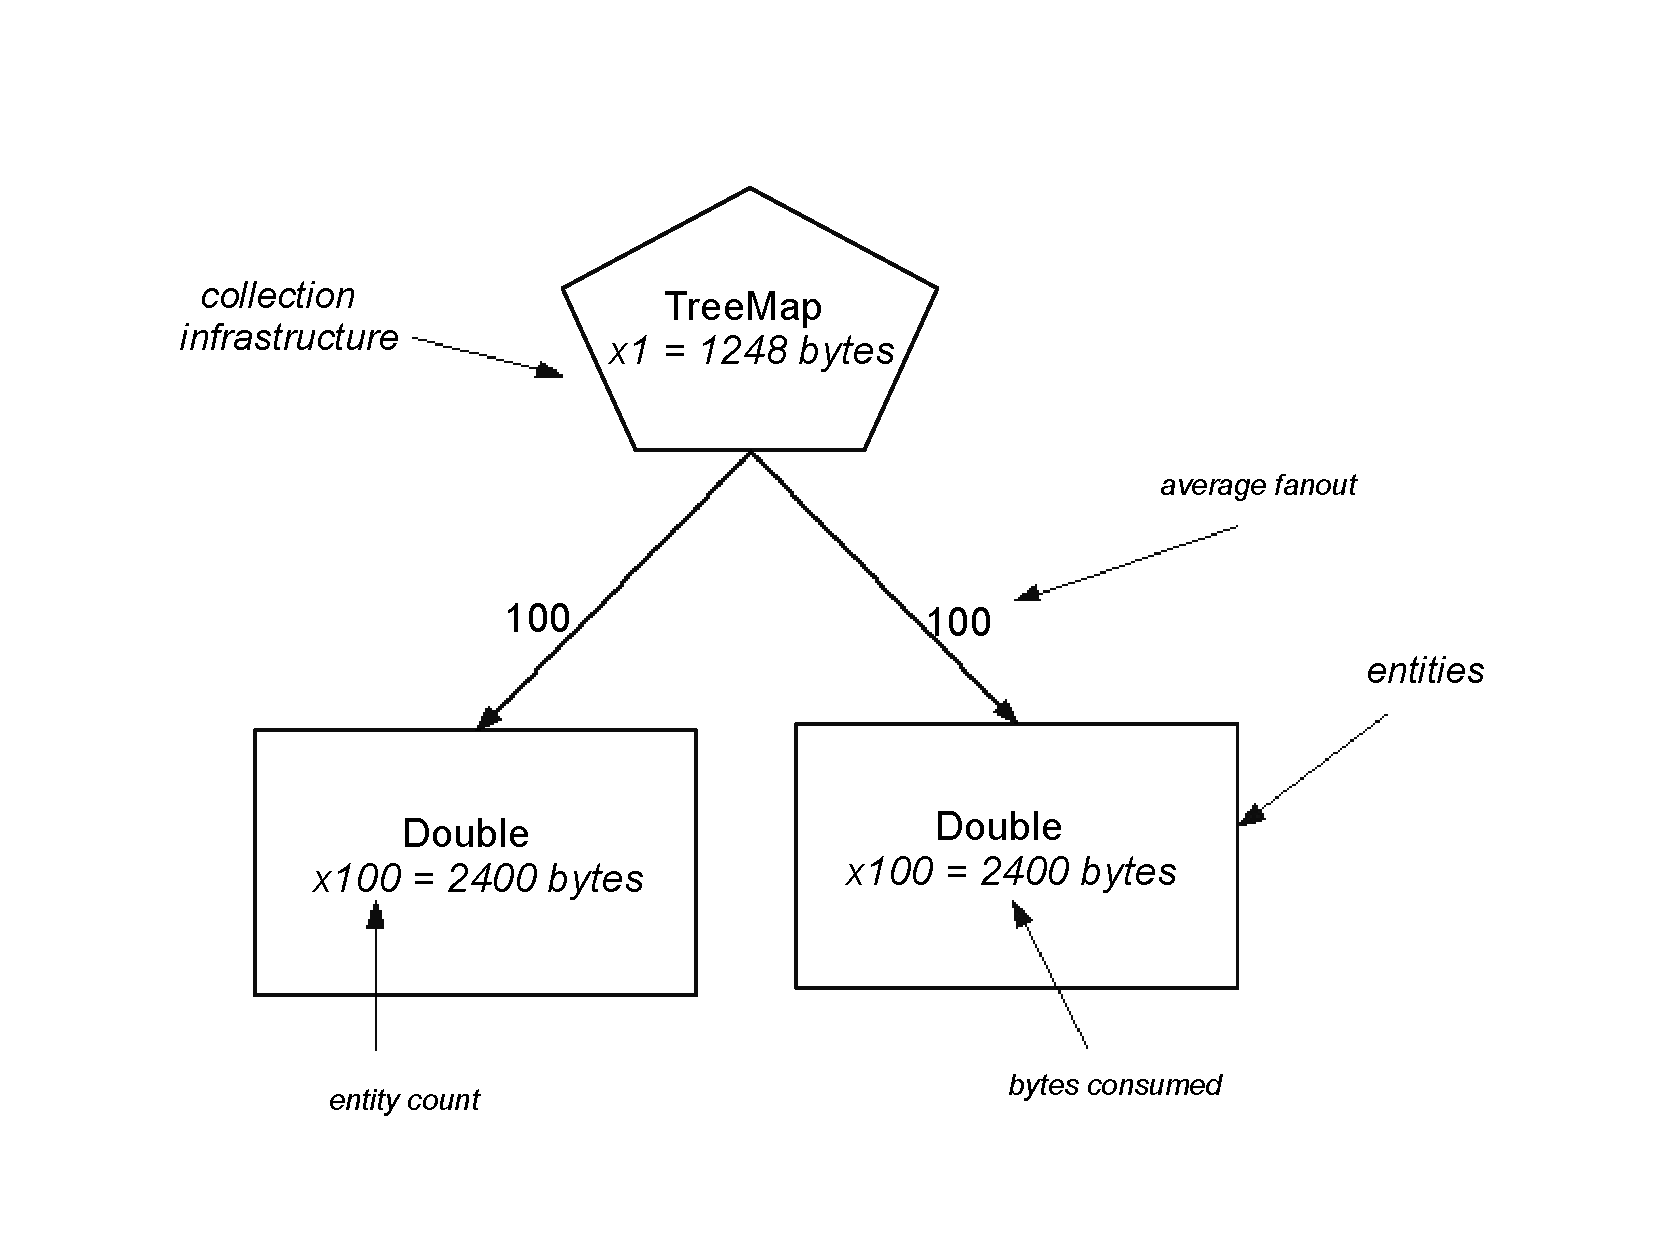
\includegraphics[width=0.7\textwidth]{part1/Figures/memoryhealth/content-schematic}
\end{center}

In an EC diagram, there are two types of boxes, pentagons and
rectangles. Each box summarizes the implementation details of a portion
of a data structure.  Pentagons represent collection infrastructure,
and rectangles represent the entities of your application.

An EC diagram represents the {\em containment} structure of your data
model. So, an edge from a collection to a rectangular entity indicates
membership of the entity in the collection. This also means that, if a
certain type of collection or entity is used in multiple ways in the
same data structure, then this type will appear in multiple locations
--- one in each location in the data structure in which that type is
used.

The notation $x N = M$ inside each node means there are $N$
objects of that type in that location in the data structure, and in
total these objects occupy $M$ bytes of memory. Each edge in a
content schematic is labeled with the average fanout from the source
entity to the target entity.
%\caption{--- The Entity-Collection (EC) Diagram}

%Notice how an EC diagram summarizes away some of the details that an
%ER diagram shows, and shows some implementation details than an ER
%diagram does not include.
%The EC diagram represents collection choices, rather than the
%relations they implement.
%where an ER diagram would show a single relation node for an M-to-N
%relation, 
Where an ER or UML diagram would show the attributes of each entity,
but ignore the implementation costs, an EC diagram summarizes the
total cost in the single sizing number shown in each node. Where these other diagrams
would show relations or roles as edges, an EC diagram shows a node summarizing the
collections implementing this relation.
%Unlike UML diagrams, relationships are elevated to be entities, rather
%than edges. The reason is that in a language like Java, implementation
%of the relationship itself is often a big cause of expense, so it is
%important to make that visible. A very common pattern is to implement
%relationships as collections. 
 }

%%%% this is the old Collection of Strings example
%In Figure~\ref{fig:content-schematic}, there are two
%\texttt{Collection}s which together occupy 200 bytes, and ten
%\texttt{String}s occupy 880 bytes. There are on average five elements
%contained in each of the two \texttt{Collection}. Since the overhead
%of a \texttt{String} is 48 bytes and there are 10 \texttt{String}s,
%the total overhead is 480 bytes or 55\%. Data occupies 400 bytes, so
%the average \texttt{String} length is 10. The two \texttt{Collection}s
%are pure overhead, so the total overhead of this data structure is 680
%bytes, or 63\%.



% The name of an entity is the name of the top object. Entities also
% summarize objects of the same type that are repeated in a data
% structure. The \texttt{String} entity in
% Figure~\ref{fig:content-schematic} represents the 10 \texttt{String}s
% in the two \texttt{Collection}s. The memory cost of an entity is the
% sum over all of its objects. This summarization removes clutter and
% helps understanding.

%\begin{figure}
%  \centering
%  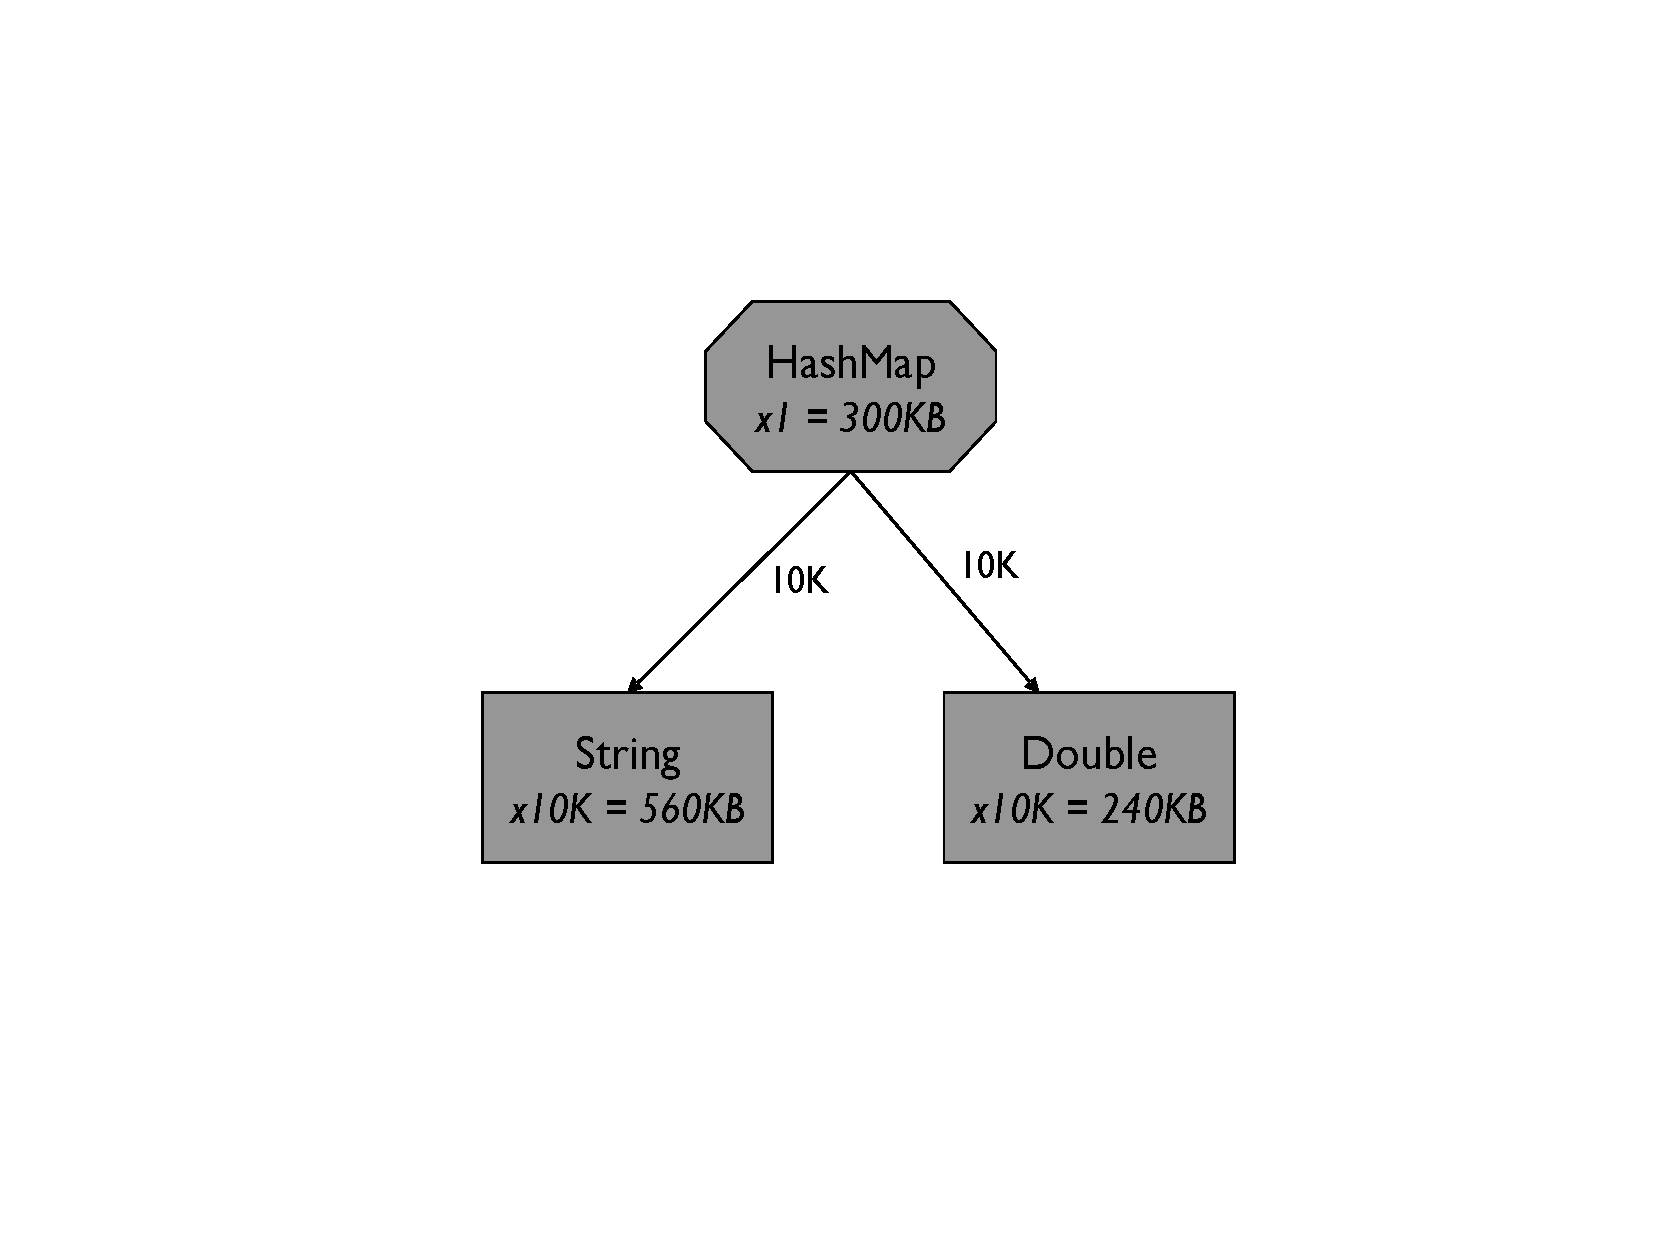
\includegraphics[width=0.9\textwidth]{Figures/content-schematic-relationship}
%  \caption{A content schematic of a map from 10K \texttt{Strings} to 10K \texttt{Doubles}.}
 % \label{fig:content-schematic-relationship}
%\end{figure}



%\section{Example: Sorted Map of Doubles}
%\label{section:mapofdoubles}

 \begin{example}{A Monitoring System}
   A monitoring program collects samples from a distributed
   system. Each sample it collects consists of a unique timestamp and a
   value, each represented as a double. The samples arrive out of
   order. The task is to display samples in chronological order, after
   all of the data has been collected. The solution requires a data
   structure to store the samples. 
\end{example}
%\emph{Load-and-Use Behavior Pattern:} load data in one phase, use the data in the next phase.


A map is a convenient way to store these timestamp-value pairs. A regular \texttt{HashMap} only solves part of the monitoring system problem. To be able to display the samples in chronological order, the entries have to be sorted by timestamp. 
The first idea that leaps forward is to use a \texttt{TreeMap}. A \texttt{TreeMap} is a map that maintains its entries in sorted order, so this appears to be a perfect choice. The only problem is the memory cost.

An EC diagram of a \texttt{TreeMap} storing 100 samples is shown in Figure~\ref{fig:content-schematic-treemap-doubles}.  This diagram gives a schematic view of the \texttt{TreeMap} and the entities it contains, along with their costs. The total cost, obtained by adding up the entity and collection costs, is 6,048 bytes. The real data consumes only 1,600 bytes of this, since a double occupies 8 bytes and there are 200 of them. Therefore, the bloat factor is 74\%.  

\begin{figure}
  \centering
  %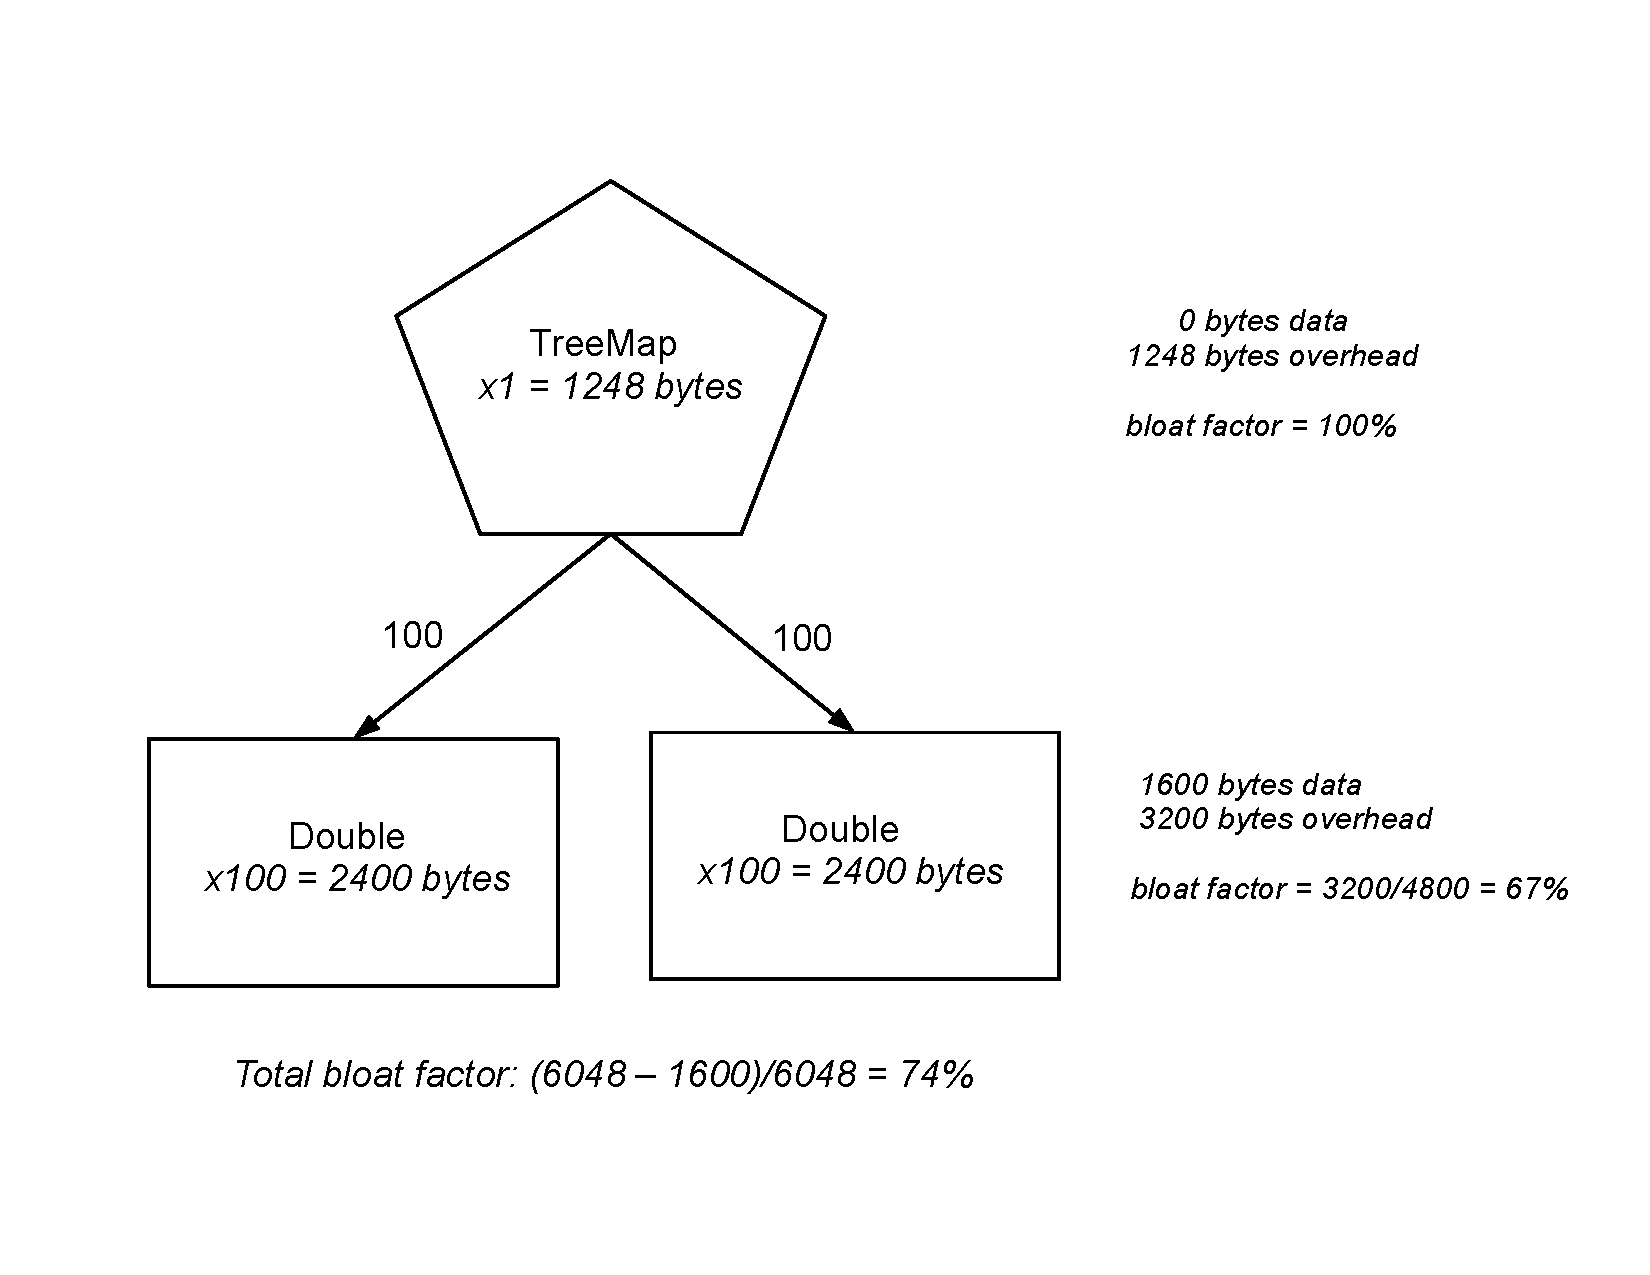
\includegraphics[width=0.4\textwidth]{Figures/treemap-doubles}
  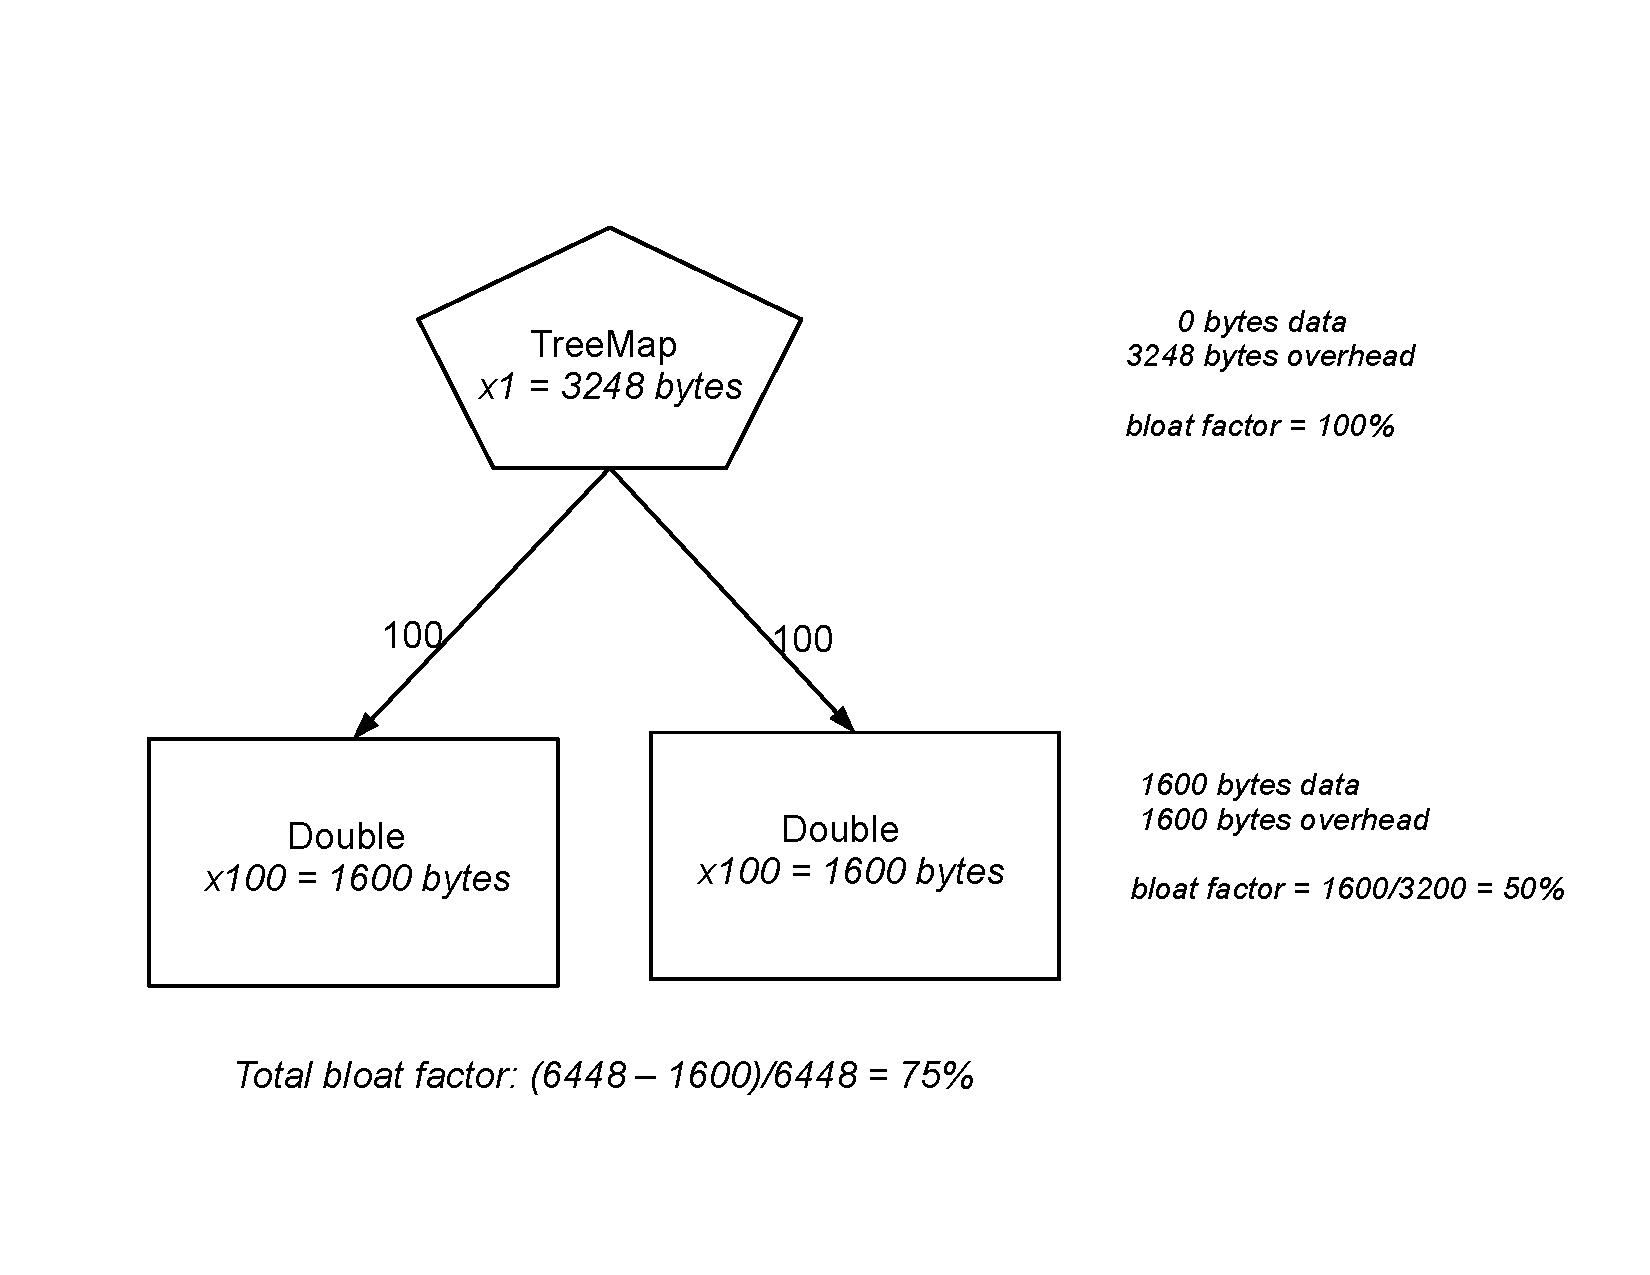
\includegraphics[width=0.7\textwidth]{part1/Figures/memoryhealth/treemap-doubles}
  \caption{EC Diagram for 100 samples stored in a \texttt{TreeMap}}
  \label{fig:content-schematic-treemap-doubles}
\end{figure} 
 
Looking at the individual parts of the EC diagram can provide some insight into the source of this overhead. First, the sample timestamps and values are stored as \texttt{Double} objects. This is because the standard Java collection APIs take only \texttt{Object}s as parameters, not scalars, forcing you to box your scalars before putting them in a collection. Even with Java's autoboxing, the compiler still generates a boxed scalar in order to store a value in a standard collection.  A single instance of a \texttt{Double} is 24 bytes, so 200 \texttt{Doubles} occupy 4,800 bytes. Since the data is only 1,600 bytes,  33\% of the \texttt{Double} objects is actual data, and 67\% is overhead. This is a high price for a basic data type. 

%A double occupies eight bytes, each sample has two doubles, so 100 samples occupy 1.6KB of actual data  -- put this into the diagramf

%Move this later? At best, the overhead will be 67\% if the doubles are boxed.

The \texttt{TreeMap} infrastructure occupies an additional 1,248 bytes of
memory. All of this is overhead. What is taking up so much space? 
\texttt{TreeMap}, like every other collection in Java, has a wrapper object, the
\texttt{TreeMap} object itself, along with other internal objects that implement
the collection functionality. Each type of collection in the standard library
has a different kind of infrastructure, some are built from arrays, some from separate entry objects linked together, and some use a combination of both. Internally, \texttt{TreeMap} is a self-balancing search tree. The tree nodes maintain pointers to parents and siblings.  In newer releases of \javasix, each node in the tree can store up to 64 key-value pairs in two arrays. This example uses this newer implementation, which is more memory-efficient for this case, but still expensive.
%    there is a separate \texttt{Treemap\$Entry} object. This is typical of collections. A typical collection has a fixed overhead, in this case it is 48 bytes, and a per-entry overhead cost, in this case it is 40 bytes per entry. These 40 bytes include five pointer fields, in addition to other sources of overhead. 

Using a \texttt{TreeMap} is not \textit{a priori} a bad design. It depends on whether the overhead is buying something useful. \texttt{TreeMap} has a high memory cost because it maintains its entries in sorted order while they are being randomly inserted and deleted. It constantly maintains a sorted order. If you need this capability, for instance, if you have a real time monitor that is constantly being updated, and you need to look at the data in order, then \texttt{TreeMap} is a great data structure.  But if you do not need this capability, there are other data structures that could provide sorted-map functionality with less memory consumption. In this example, the data needs to be sorted only after data collection is complete. There is an initial load phase followed by a use phase. The sorted order is only needed during the second phase, after all the data is loaded. This load-and-use behavior is a common pattern, and it can be exploited to choose a more memory-efficient representation.

Of course, another nice aspect of \texttt{TreeMap} is that it can be pulled off the shelf. It would be ideal if there were another collection that provides just the needed functionality. If not, maybe there is a way to easily extend another collection class by adding a thin wrapper around it. Writing your own collection class from scratch should rarely be necessary, and is not recommended.

\section{Two Memory-Efficient Designs}
\label{sec:better-designs} 

This section describes two other data structure designs to store the monitoring system samples. These designs use less memory and do not maintain sorted order while the data is being loaded. This is not a problem, since the data can be sorted after loading. 

The first design stores the samples in an \texttt{ArrayList}, where each entry is a \texttt{Sample} object containing a timestamp and value. Both values are stored in primitive \texttt{double} fields of \texttt{Sample}.  There is a bit more code that has to be written, but it is not excessive. Fortunately, the standard Java \texttt{Collections} class has some useful static methods so that new sort and search algorithms do not have to be implemented. The \texttt{sort} and \texttt{binarySearch} methods from \texttt{Collections} each can take an \texttt{ArrayList} and a \texttt{Comparable} object as parameters. To take advantage of these methods, the new \texttt{Sample} class has to implement the \texttt{Comparable} interface, so that two sample timestamps can be compared:  

\ttfamily
\begin{verbatim}
   
    public class Sample implements Comparable<Sample> {

        private final double timestamp;
        private final double value;
	
        public Sample(double timestamp, double value) {
            this.timestamp = timestamp;
            this.value = value;
        }
	
        public double getTimestamp() {
            return timestamp;
        }
	
        public double getValue() {
            return value;
        }
	      
        public int compareTo(Sample that) {
            return Double.compare(this.getTimestamp(), that.getTimestamp());	
        }
    }

\end{verbatim}
\normalfont
Additionally, the \texttt{ArrayList} needs to be stored in a wrapper class that implements map operations. Here are two methods, \texttt{getValue} and \texttt{sort}, of a wrapper class \texttt{Samples}. 
\ttfamily
\begin{verbatim}
    public class Samples {
    
    	  public final static double NOT_FOUND = -1d;
        private ArrayList<Sample> samples = new ArrayList<Sample>();
        ....
		
        public double getValue(double timestamp) {
            Sample sample = new Sample(timestamp, 0.0);
            int result = Collections.binarySearch(samples, sample);
            if (result < 0) {
            	return NOT_FOUND;
            }
            return samples.get(result).getValue();
        }
		
        public void sort() {
            Collections.sort(samples);
            samples.trimToSize();	
        }
    }
    
\end{verbatim}
\normalfont 
  
The EC diagram for 100 entries is shown in Figure~\ref{fig:content-schematic-arraylist-pairs}.
\begin{figure}
  \centering
 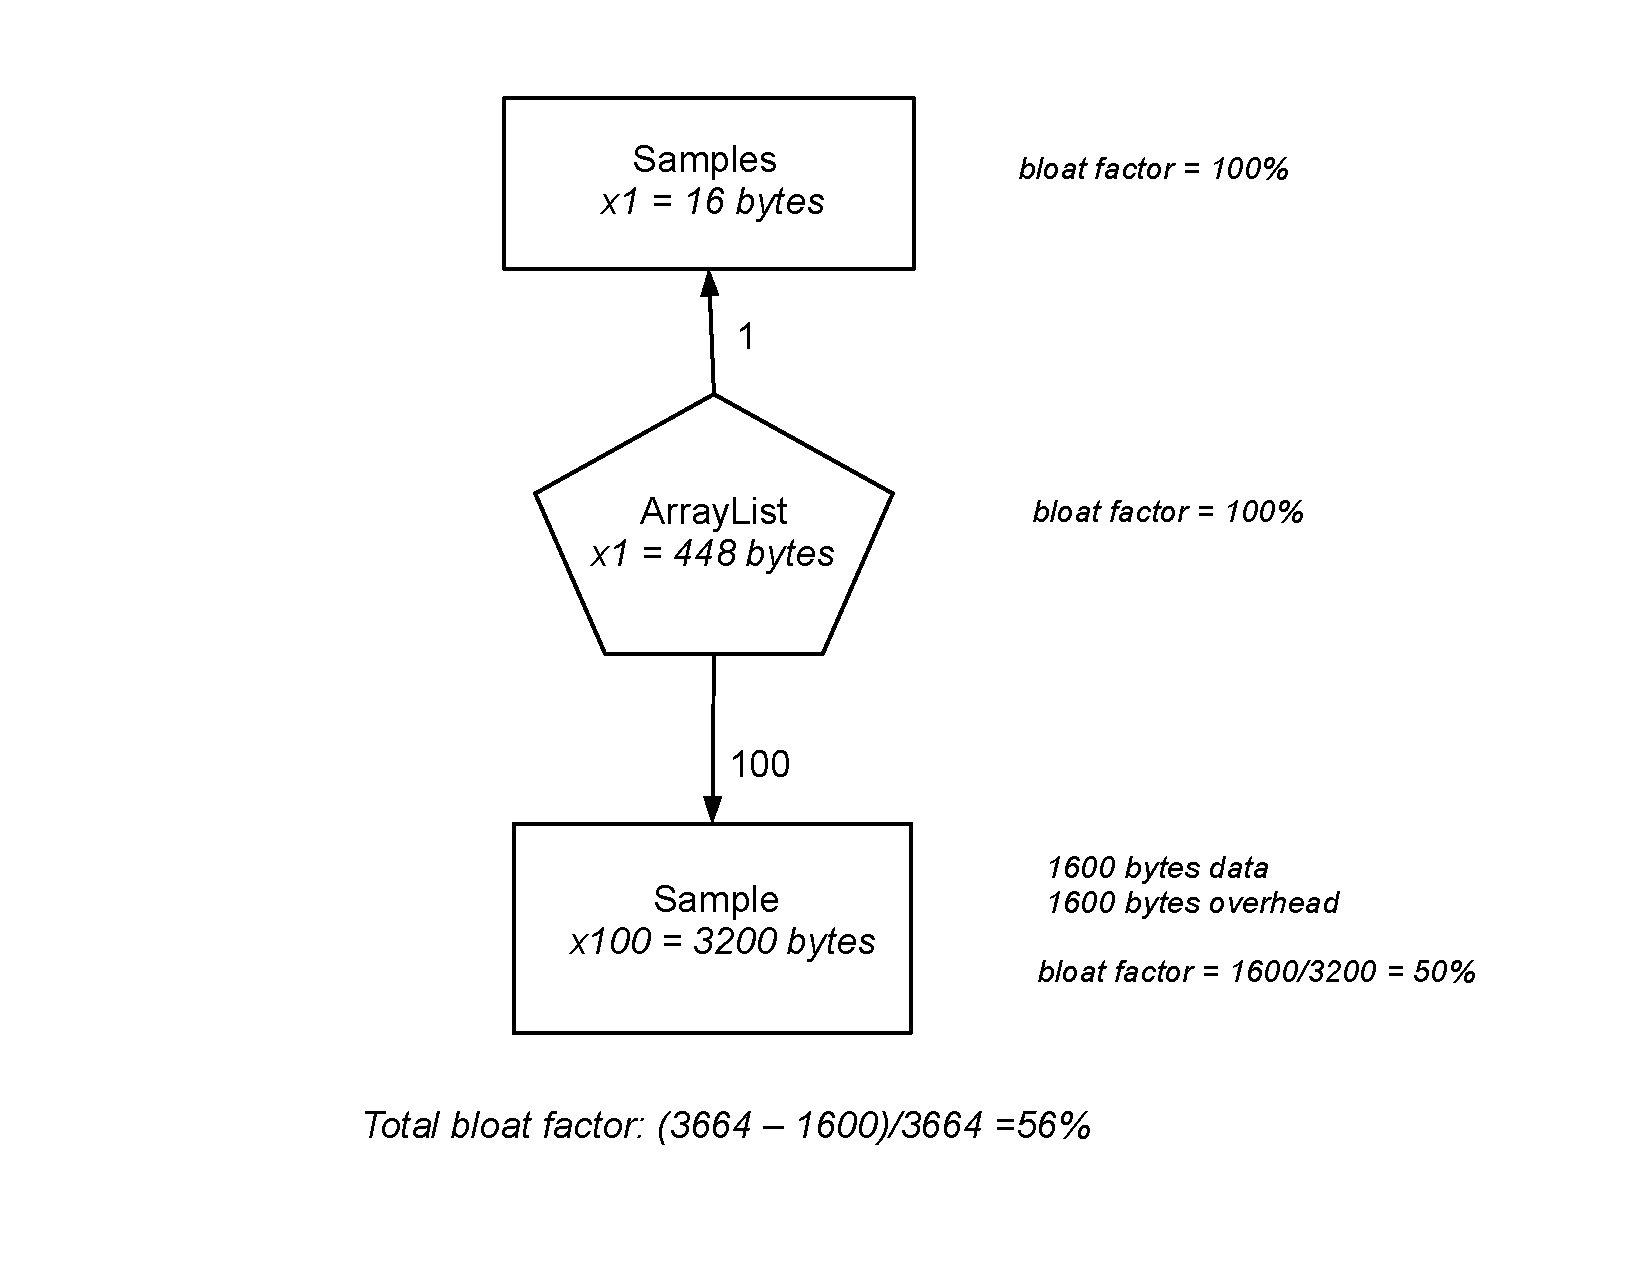
\includegraphics[width=0.7\textwidth]{part1/Figures/memoryhealth/arraylist-doubles}
  \caption{EC Diagram for 100 samples stored in an \texttt{ArrayList} of \texttt{Samples}}
  \label{fig:content-schematic-arraylist-pairs}
\end{figure} 
This design uses less memory and has better health than the \texttt{TreeMap} design. The memory cost is reduced from 6,048 to 3,664 bytes, and the overhead is reduced from 74\% to 56\%.  There are two reasons for this improvement. First, the timestamps and values are not boxed. They are stored as primitive double fields in each \texttt{Sample}. This reduces the number of objects needed to store the actual data from 200 to 100. Fewer objects means fewer object headers and pointers, which is significant in this case. Secondly, an \texttt{ArrayList} has lower infrastructure cost than a \texttt{TreeMap}. \texttt{ArrayList} is one of the most memory-efficient Java collections. It is implemented using a wrapper object and an array of pointers. This is much more compact than the heavy-weight \texttt{TreeMap}. 

While this is a big improvement, 56\% overhead still seems high. Over half the memory is being wasted. How hard is it to get rid of this overhead completely? Eliminating overhead means eliminating objects altogether. This is not a recommended practice, unless memory is extremely tight, and there is no other choice. It is none the less an interesting exercise to compare a best case design with the other designs. The most space-efficient design uses two parallel arrays of doubles. One array stores all of the sample timestamps, and the second stores all of the values. These arrays can be stored in a wrapper class that implements a map interface.

This design requires a bit more code, but, again, it is not excessive. Like the \texttt{Collections} class, the \texttt{Arrays} class provides static \texttt{sort} and  \texttt{binarySearch} methods. However, these methods apply only to a single array. If you sort the timestamp array, you will lose the association between the timestamps and their corresponding values. You can use an extra temporary array to get around this problem. The implementation is left as an exercise. The EC diagram for this design using two double arrays is shown in 
Figure~\ref{fig:content-schematic-arrays-doubles}. The overhead is only 4\%. 

\begin{figure}
  \centering
  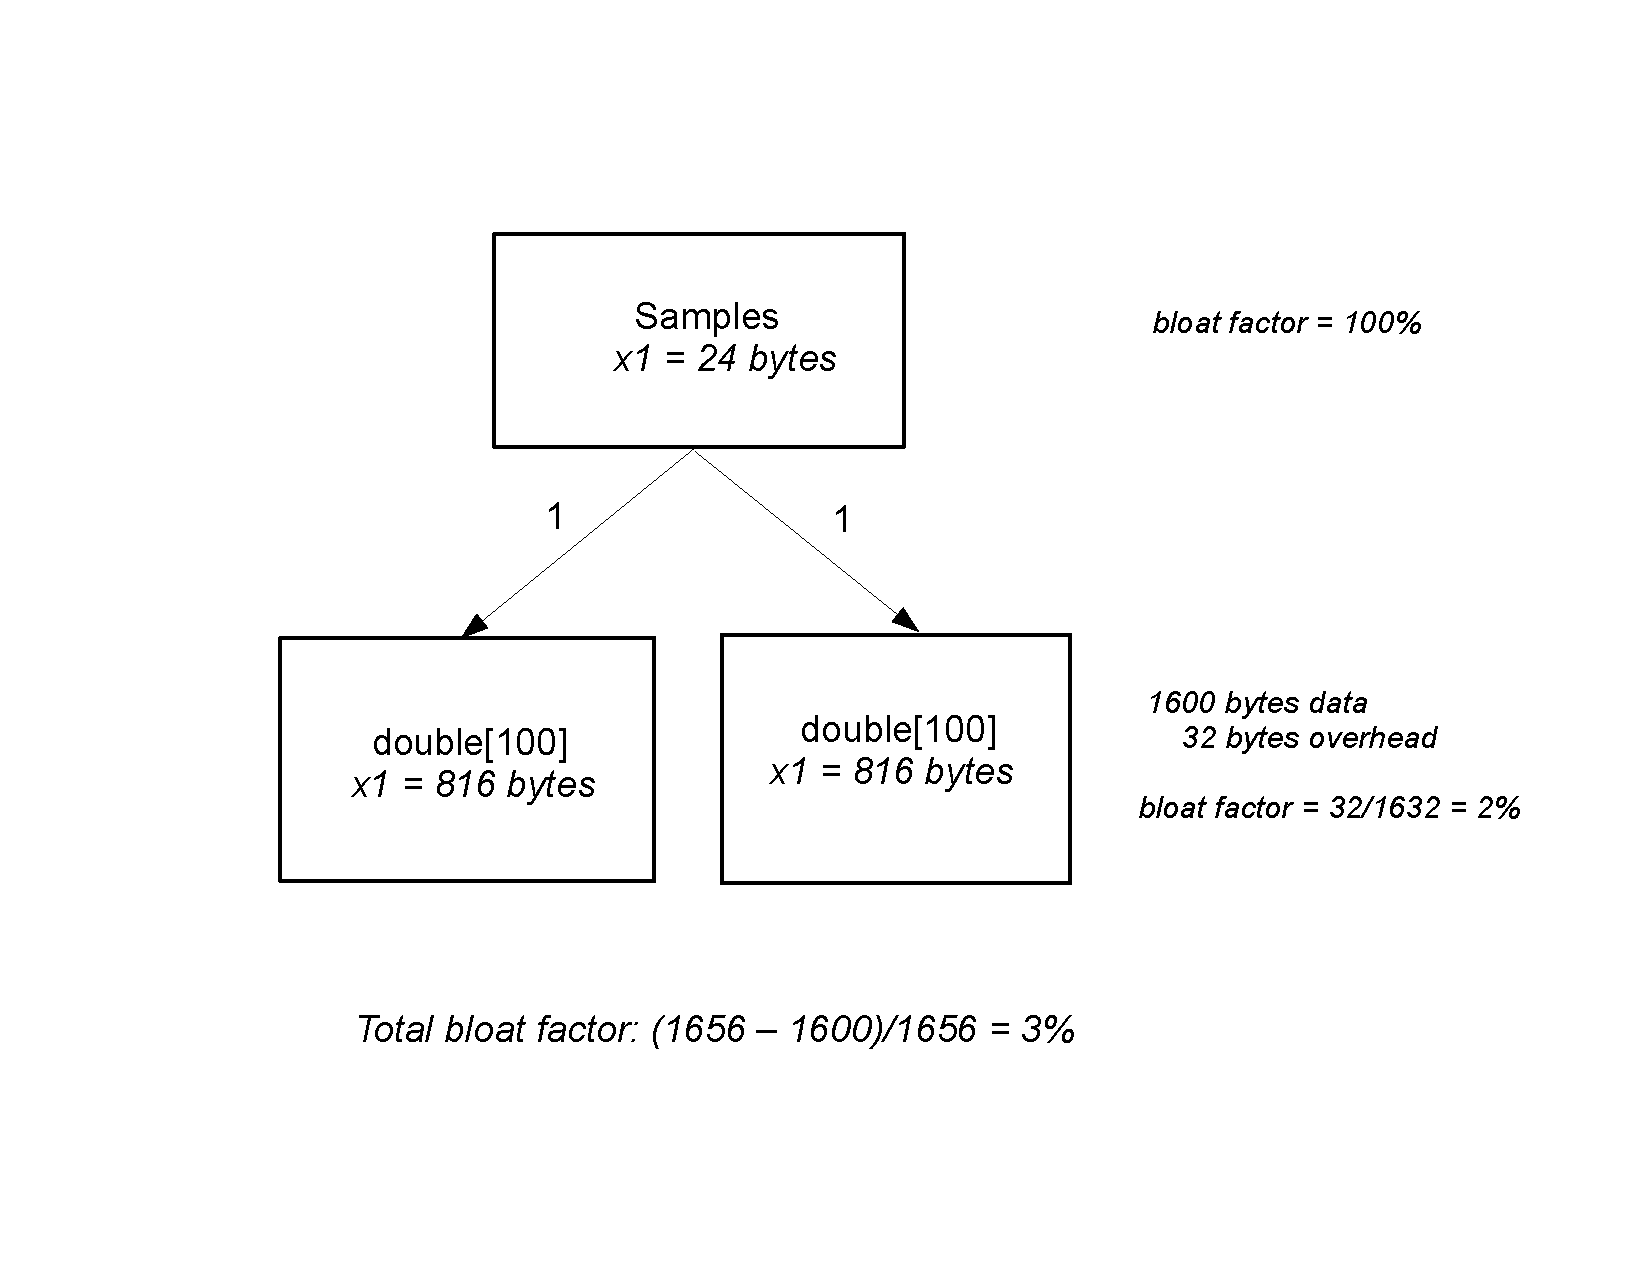
\includegraphics[width=0.7\textwidth]{part1/Figures/memoryhealth/array-doubles}
  \caption{EC Diagram for 100 samples stored in two parallel arrays}
  \label{fig:content-schematic-arrays-doubles}
\end{figure}

For the three designs presented, there is a tradeoff between ease of programming and memory efficiency. More programming is needed as the design becomes more memory efficient. However, in many cases, memory efficient designs are just as easy to implement as inefficient designs. When there are two distinct execution phases, as in this example, the data structure can be trimmed after the first phase, to eliminate empty space reserved for growth. Another option is to use one data structure in the first phase, and copy it into a second data structure for the second phase. This approach can sometimes be a good compromise between ease-of-programming and memory efficiency.
 
\section{Scalability}
\label{sec:scalability}

The evaluation of the three monitoring system designs was based on only 100 samples. In a real scenario, a monitoring system might have to handle hundreds of thousands, or millions, of samples. Stress testing is usually performed late in a development cycle, when it is very costly to fix a memory footprint problem. Using a memory health approach, it possible to predict how well a data structure design will scale much earlier.
 
\begin{figure}
  \centering
   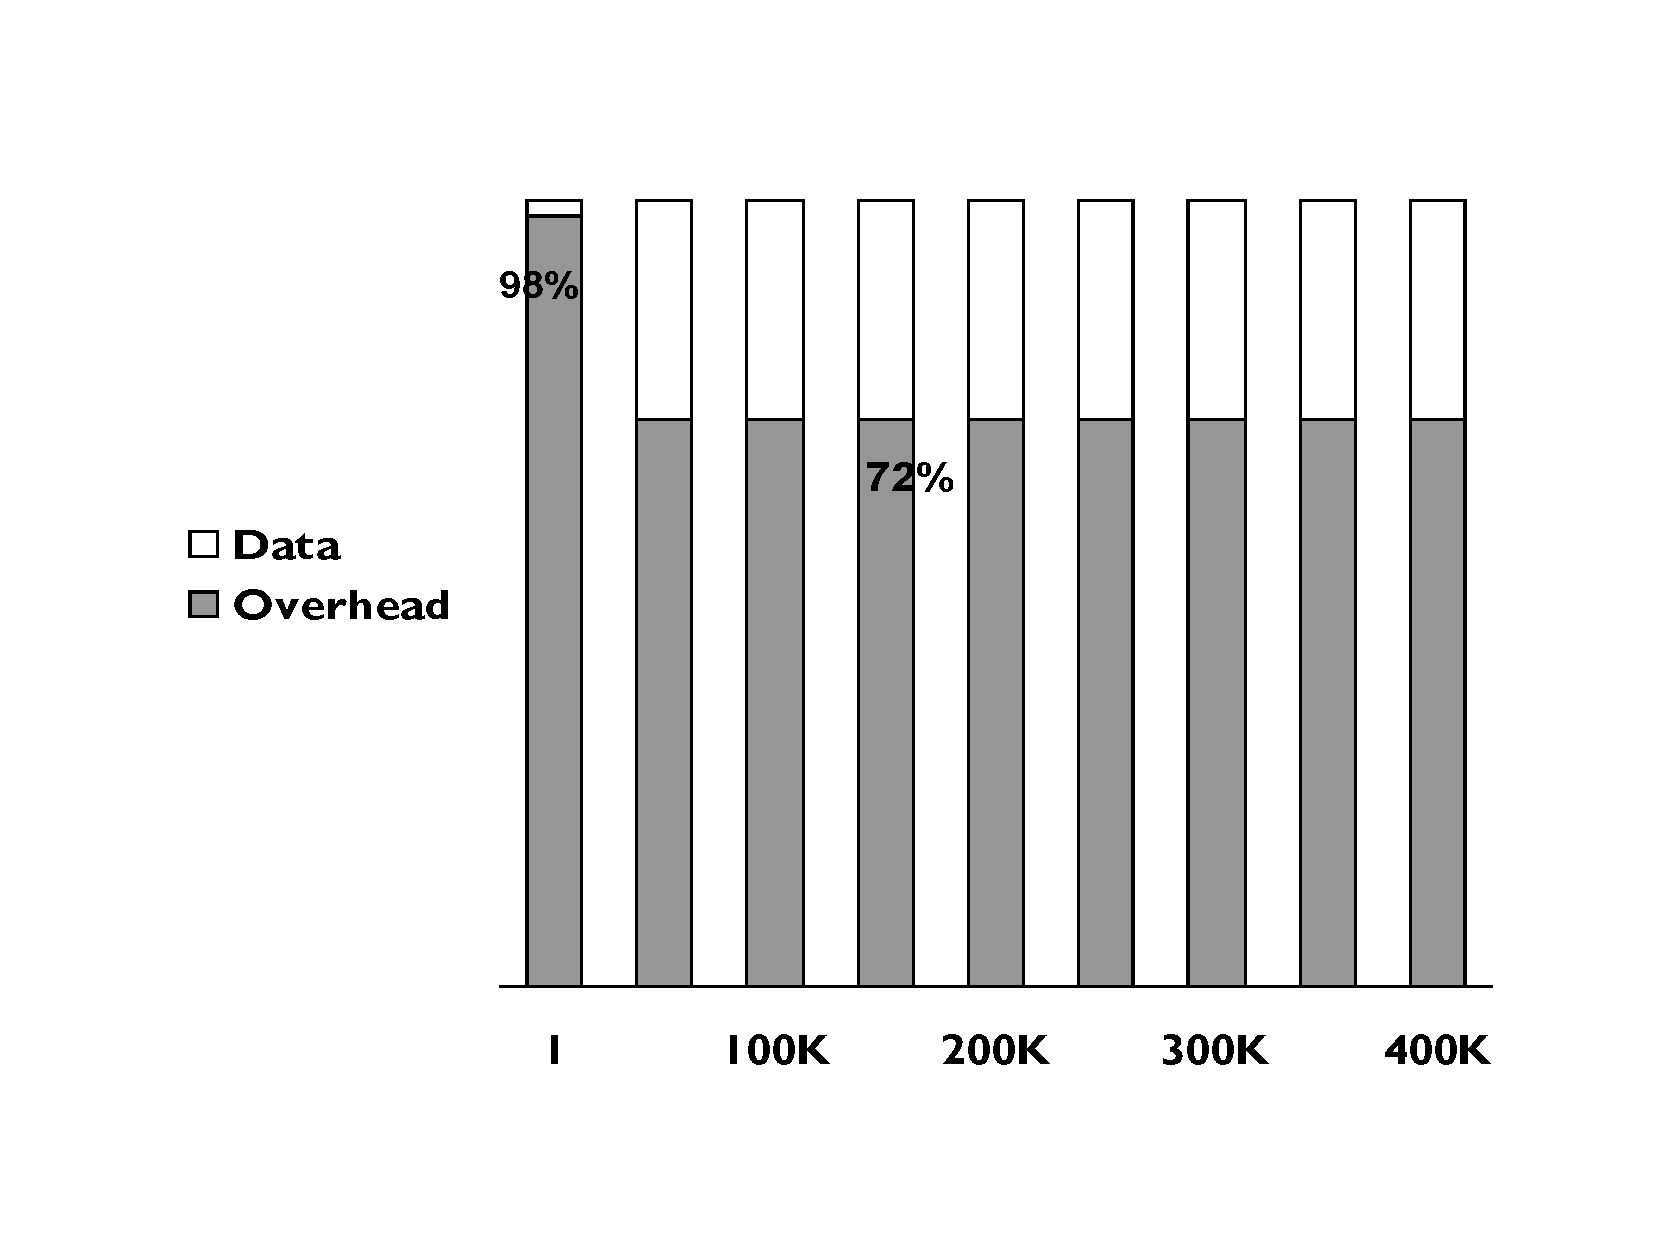
\includegraphics[width=0.7\textwidth]{part1/Figures/memoryhealth/scalable-health-treemap}
  \caption{Health Measure for the \texttt{TreeMap} Design Shows Poor Scalability}
  \label{fig:scalable-health-treemap}
\end{figure}
The basic question for predicting scalability is what happens to the bloat factor as a data structure grows. The \texttt{TreeMap} design has 74\% overhead with 100 samples. With 100,000 samples, maybe the high overhead will be amortized away, that is, maybe this design will scale well, even if it is inefficient for small data sizes. The bar graph in Figure~\ref{fig:scalable-health-treemap} shows how the \texttt{TreeMap} design scales as the number of samples increase. Each bar is split into two parts: the percentage of overhead and the percentage of data. For a single sample, the overhead is 98\%! As more samples are added, the bloat factor drops to 72\%. Unfortunately, with 200,000 samples, and 300,000 samples, the bloat factor is still 72\%. The \texttt{TreeMap} design is not only bloated, but it also does not scale. It is constantly bloated.

To understand why this happens, recall that the infrastructure of \texttt{TreeMap} is made up of nodes, with two 64-element arrays hanging off of each node. As samples are added, the infrastructure grows, since new nodes and arrays are being created. Also, each additional sample has its own overhead, namely the JVM overhead in each \texttt{Double} object. When the \texttt{TreeMap} becomes large enough, the \textit{per-entry overhead} dominates and hovers around 72\%. The bloat factor is larger when the \texttt{TreeMap} is small. In contrast, for small \texttt{TreeMap}s, the fixed cost of the initial \texttt{TreeMap} infrastructure is relatively big. The \texttt{TreeMap} wrapper object alone is 48 bytes. This initial fixed cost is quickly amortized away as samples are added. 

\callout{callout:fixed-and-per-entry-costs}{Fixed vs Per-Entry Overhead}{
\index{Fixed Collection Overhead} \index{Per-Entry Collection Overhead}
The memory overhead of a collection can be classified as either \textit{fixed} or \textit{per-entry}. Fixed overhead stays the same, no matter how many entries are stored in the collection. Small collections with a large fixed overhead have a high memory bloat factor, but the fixed overhead is amortized away as the collection grows. Per-entry overhead depends on the number of entries stored in the collection. Collections with a large per-entry overhead do not scale well, since per-entry costs cannot be amortized away as the collection grows. 
}

\begin{figure}
  \centering
   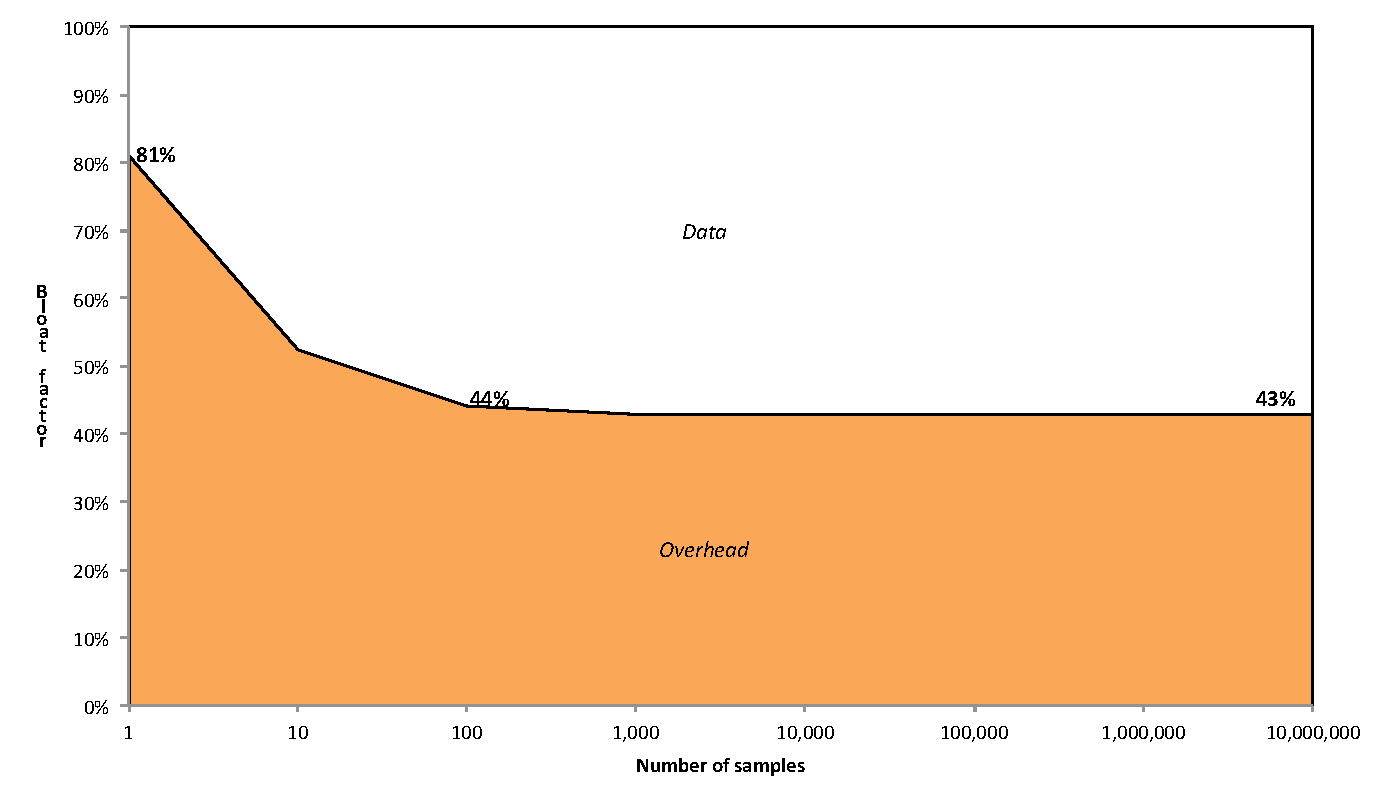
\includegraphics[width=0.7\textwidth]{part1/Figures/memoryhealth/scalable-health-arraylist}
  \caption{Health Measure for the \texttt{ArrayList} Design }
  \label{fig:scalable-health-arraylist}
\end{figure}

Figure~\ref{fig:scalable-health-arraylist} shows similar data for the \texttt{ArrayList} design. Like the \texttt{TreeMap} design, there is a fixed overhead, which is significant when the \texttt{ArrayList} is small. As the \texttt{ArrayList} grows, the fixed overhead is amortized away, but there is still a per-entry cost of 56\%, that remains constant. 

For the last design that uses arrays, there is only fixed overhead, namely, the \texttt{Samples} object and JVM overhead for the arrays. There is no per-entry overhead at all. Figure~\ref{fig:scalable-health-array} shows the initial 80\% fixed overhead is quickly amortized away. When more samples are added, the bloat factor becomes 0. The samples themselves are pure data.

\begin{figure}
  \centering
  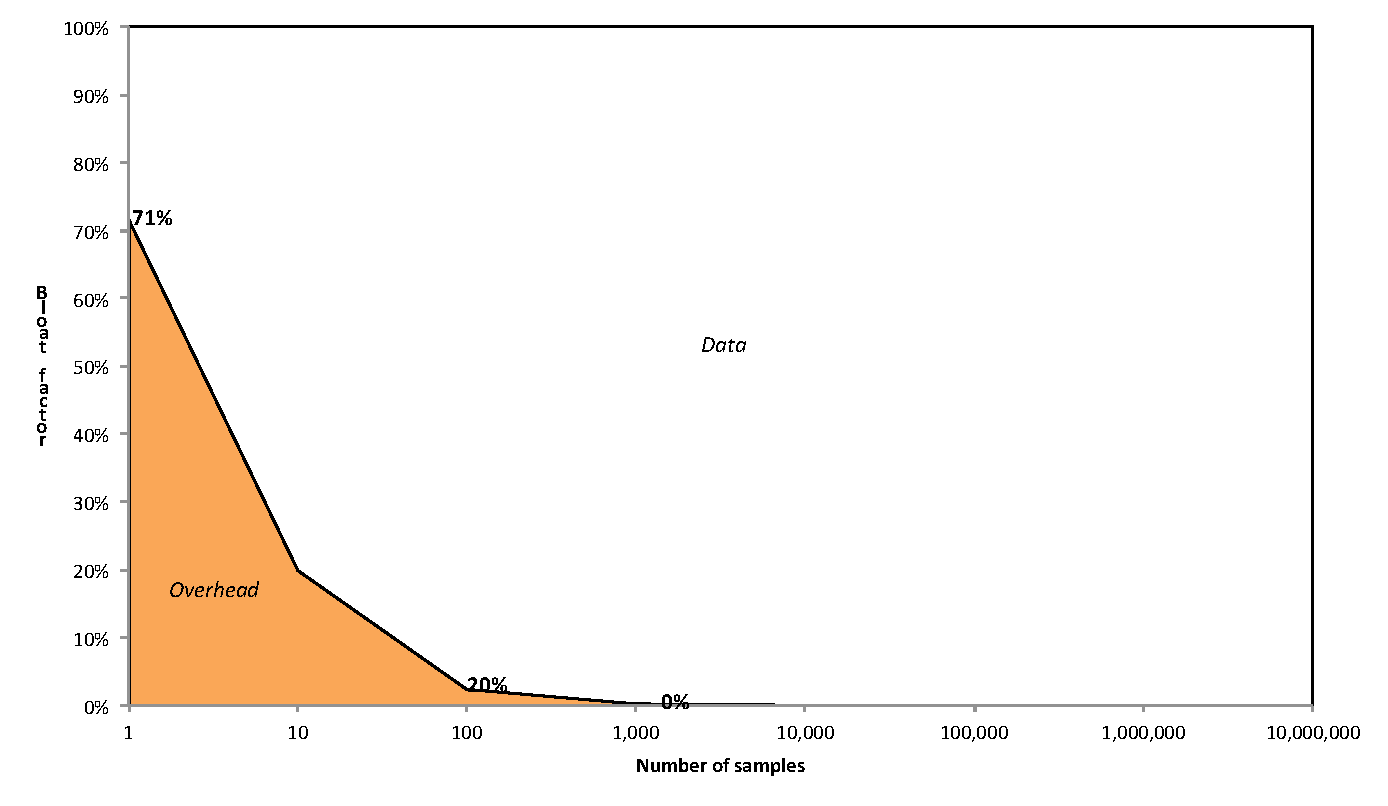
\includegraphics[width=0.7\textwidth]{part1/Figures/memoryhealth/scalable-health-array}
  \caption{Health Measure for the Array-Based Design Shows Perfect Scalability}
  \label{fig:scalable-health-array}
\end{figure}

This analysis helps predict the memory requirements for large sample sizes. Suppose the monitoring system needs to process 10 million samples. The data alone takes up 160 million bytes (153MB).  The graphs shown in this section can be used to quickly calculate how much memory you will need. For the \texttt{TreeMap} design, the overhead cost is 72\%, so you will need 546MB to store the samples. For the \texttt{ArrayList} design, you will need 347MB. For the \texttt{array} design, you will need only 153MB. As these numbers show, the design choice can make a huge difference.

\section{Summary}

When you are developing a large application, closing your eyes to quantitative considerations and thinking everything is going to be fine is risky. Taking the time to measure the cost and health of your data design can pinpoint problems early on. This chapter described three conceptual tools to help evaluate the memory-efficiency of a design.
\begin{itemize}
\item The \textsl{memory bloat factor} measures how much of your the memory usage of your design is real data, and how much is an artifact of the way you have chosen to represent it. This metric tells you how much room there is for improvement, and if in fact you are paying a reasonable price for what you are getting.
\item Complex data structures are built up from data entities and collections of these entities.  The \textsl{Entity-Collection (EC) Diagram} shows the costs associated with the different parts of a complex data structure. These diagrams help you to compare the memory efficiency of different representation choices.
\item By classifying the overhead of a collection as either \textsl{fixed} or \textsl{per-entry}, you can predict how much memory you will need to store very large collections. Being able to predict scalability is critical to meeting the requirements of larges applications. 
\end{itemize}
These are the basic tools used in the rest of this book. To estimate the cost of an entity, you will need to know how many bytes each primitive type needs, what is the pointer size, and what the JVM overhead is. You will learn how to estimate the cost of entities in Chapter 4. To estimate scalability, you will need to know what the fixed and per-entry costs are for the collection classes you are using. These are given in Chapter 7.

%Nevertheless, you should not throw out all the Java libraries and write everything yourself.  It can also prevent unnecessary optimizations that gain little or nothing. You should perform thought experiments, use limit cases to understand optimal designs, and make back-of-the-envelope calculations.  This requires more work, possibly more prototyping, but the effort will likely pays off. Subsequent chapters discuss more techniques for precise estimation of memory health, and provide the data and overhead costs of common primitives and collections needed to perform estimations. 

\chapter{Objects and Delegation}
\label{chapter:delegation}

An important design decision when modeling data is how many Java classes to use to represent a logical concept.
The choices made at this design stage can impact memory costs significantly. At one extreme, a single class may store
all attributes. At the other extreme, a main class may delegate many of its attributes to other classes,
resulting in a fine-grained design. Delegation is a very popular pattern because of the flexibility it provides.
It is also one of the few ways Java allows you to reuse existing classes. Yet, overly fine-grained data models
can result in poor memory health. This chapter explains how to evaluate the granularity of a design from a memory perspective.
It begins with the costs of basic objects, and moves on to examples from real applications.
  
\section{The Cost of Objects}
\label{sec:CostOfObjects}

There is no Java library method that returns the size of an object. This is by
design. Unlike systems languages like C, a Java programmer is not supposed to
know either the size of an object or how it is laid out in memory. The \jre,
not the programmer, manages storage, and the \jre has the freedom to implement
its own storage policy. However, knowing the sizes of objects is necessary for understanding
memory requirements and scalability. Fortunately, it is not hard to estimate the size of an object,
and a good estimate of the most prevelant classes is usually sufficient for making intelligent design choices.
You need to know just a few basics, starting with the number of bytes needed to store primitive data types.
These sizes are defined in the Java language specification~\cite{JavaSpec}, and are given in Table~\ref{tab:primitive-sizes}.
Fields can also be reference fields, pointing to other objects. Their size
depends on the architecture of the \jre. They are 4 bytes on a 32-bit \jre.
\begin{table}
  \centering
%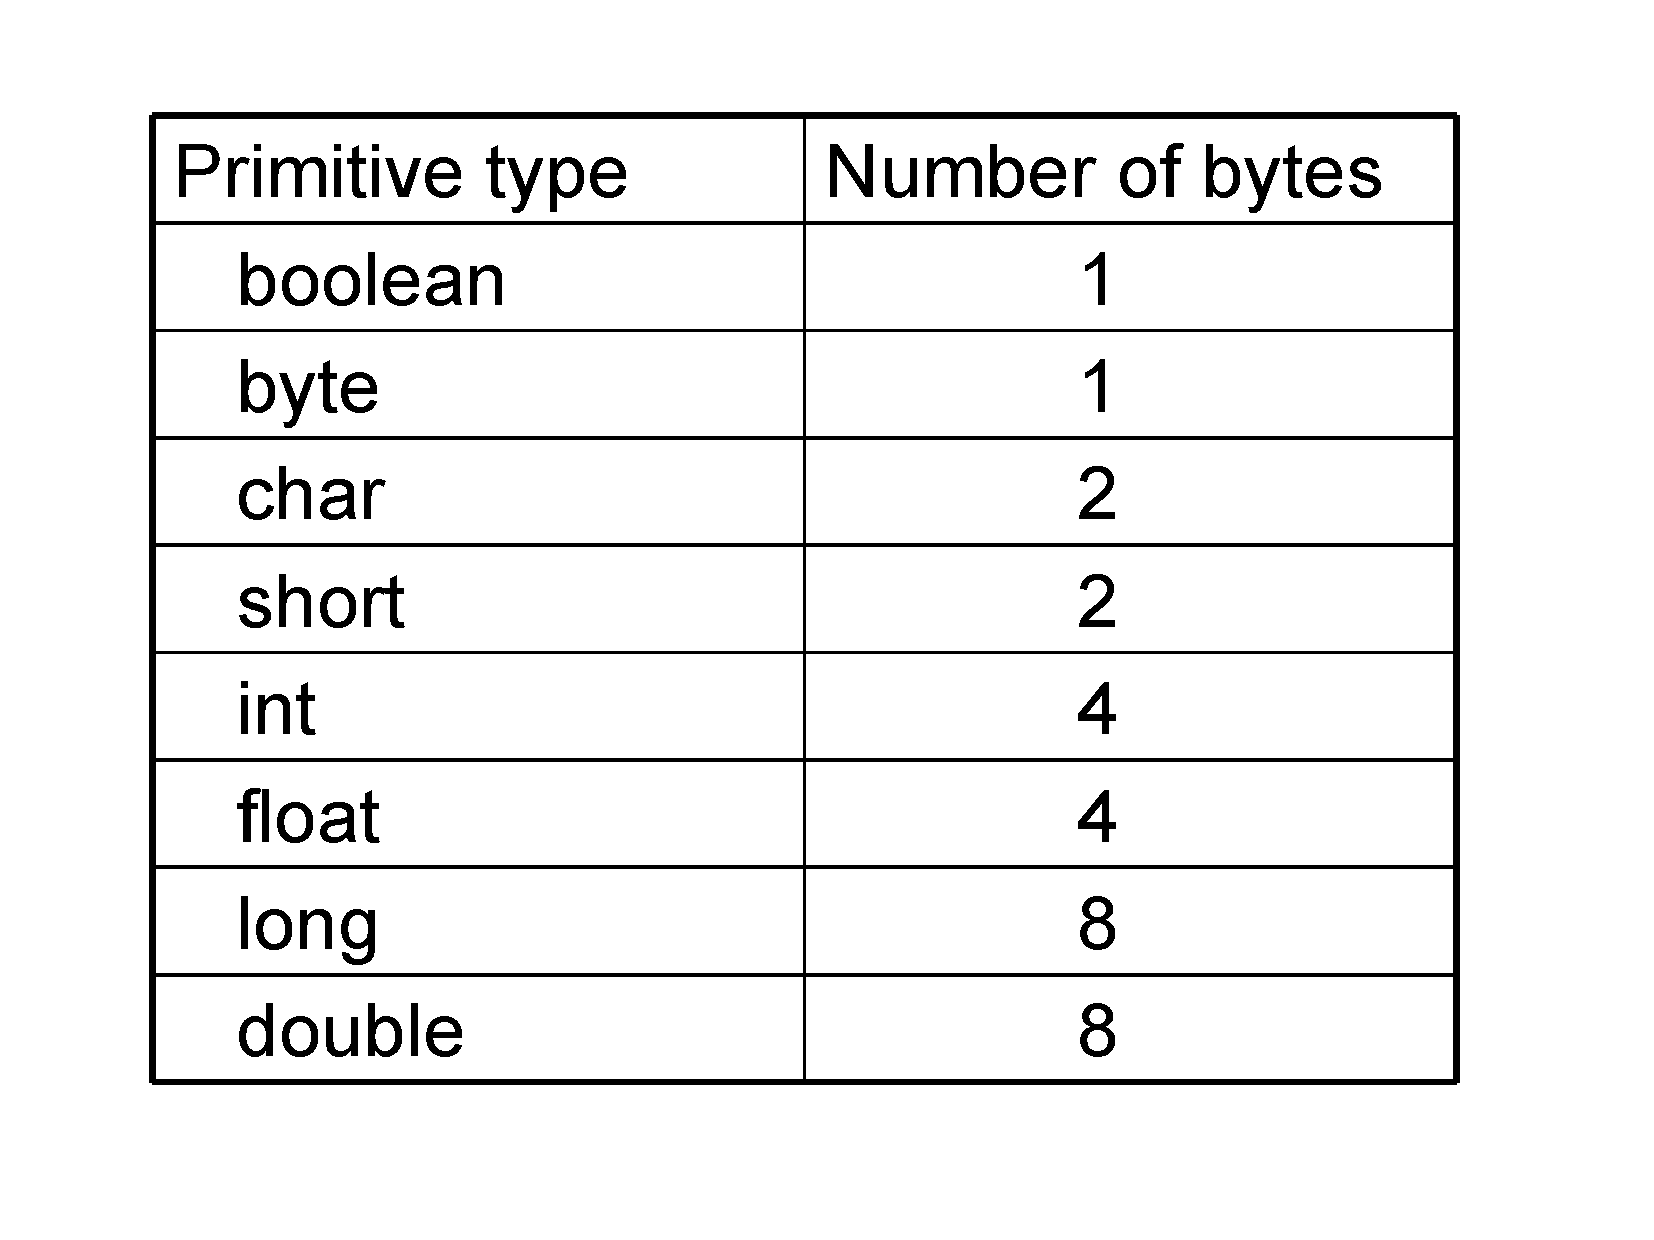
\includegraphics[width=.50\textwidth]{part1/Figures/modelingdatatypes/primitive-byte-sizes.pdf}
\begin{tabular}{lc} \toprule
	Data type & Number of bytes \\ \midrule
	primitives \\ \midrule
	boolean, byte & 1 \\
	char, short & 2 \\
	int, float & 4 \\
	long, double & 8 \\ \midrule
	reference (32-bit \jre) & 4 \\
	\bottomrule
\end{tabular}
 % \includegraphics{eight-char-string}
  \caption{The number of bytes needed to store primitive data and reference
  fields.}
  \label{tab:primitive-sizes}
\end{table}

\paragraph{Object-level overhead} Objects are bigger than the sum of their
fields, and their size depends on the specific \jre implementation. The \jre allocates a header with each object that
stores information such as the object's class, an identity hashcode, a monitor
used for locking, and various flags. For array objects, the header has an
additional integer to store the number of array elements. Additionally,  the
\jre requires objects to be aligned on specific address boundaries, for example,
addresses that are multiples of 8. To show how implementations differ,
Table~\ref{tab:object-overhead} gives object header and alignment costs imposed
by two \jres, Sun \javasix (Update 14) and IBM \javasix (Service Release 4),
both for 32-bit architectures. \footnote{Unless otherwise noted, all of the
numbers throughout the book are based on the Sun \jre for 32-bit architectures.
Appendix~\ref{chapter:jre-comparison} gives information needed to estimate
sizes in various environments.}
\begin{table}
  \centering
 %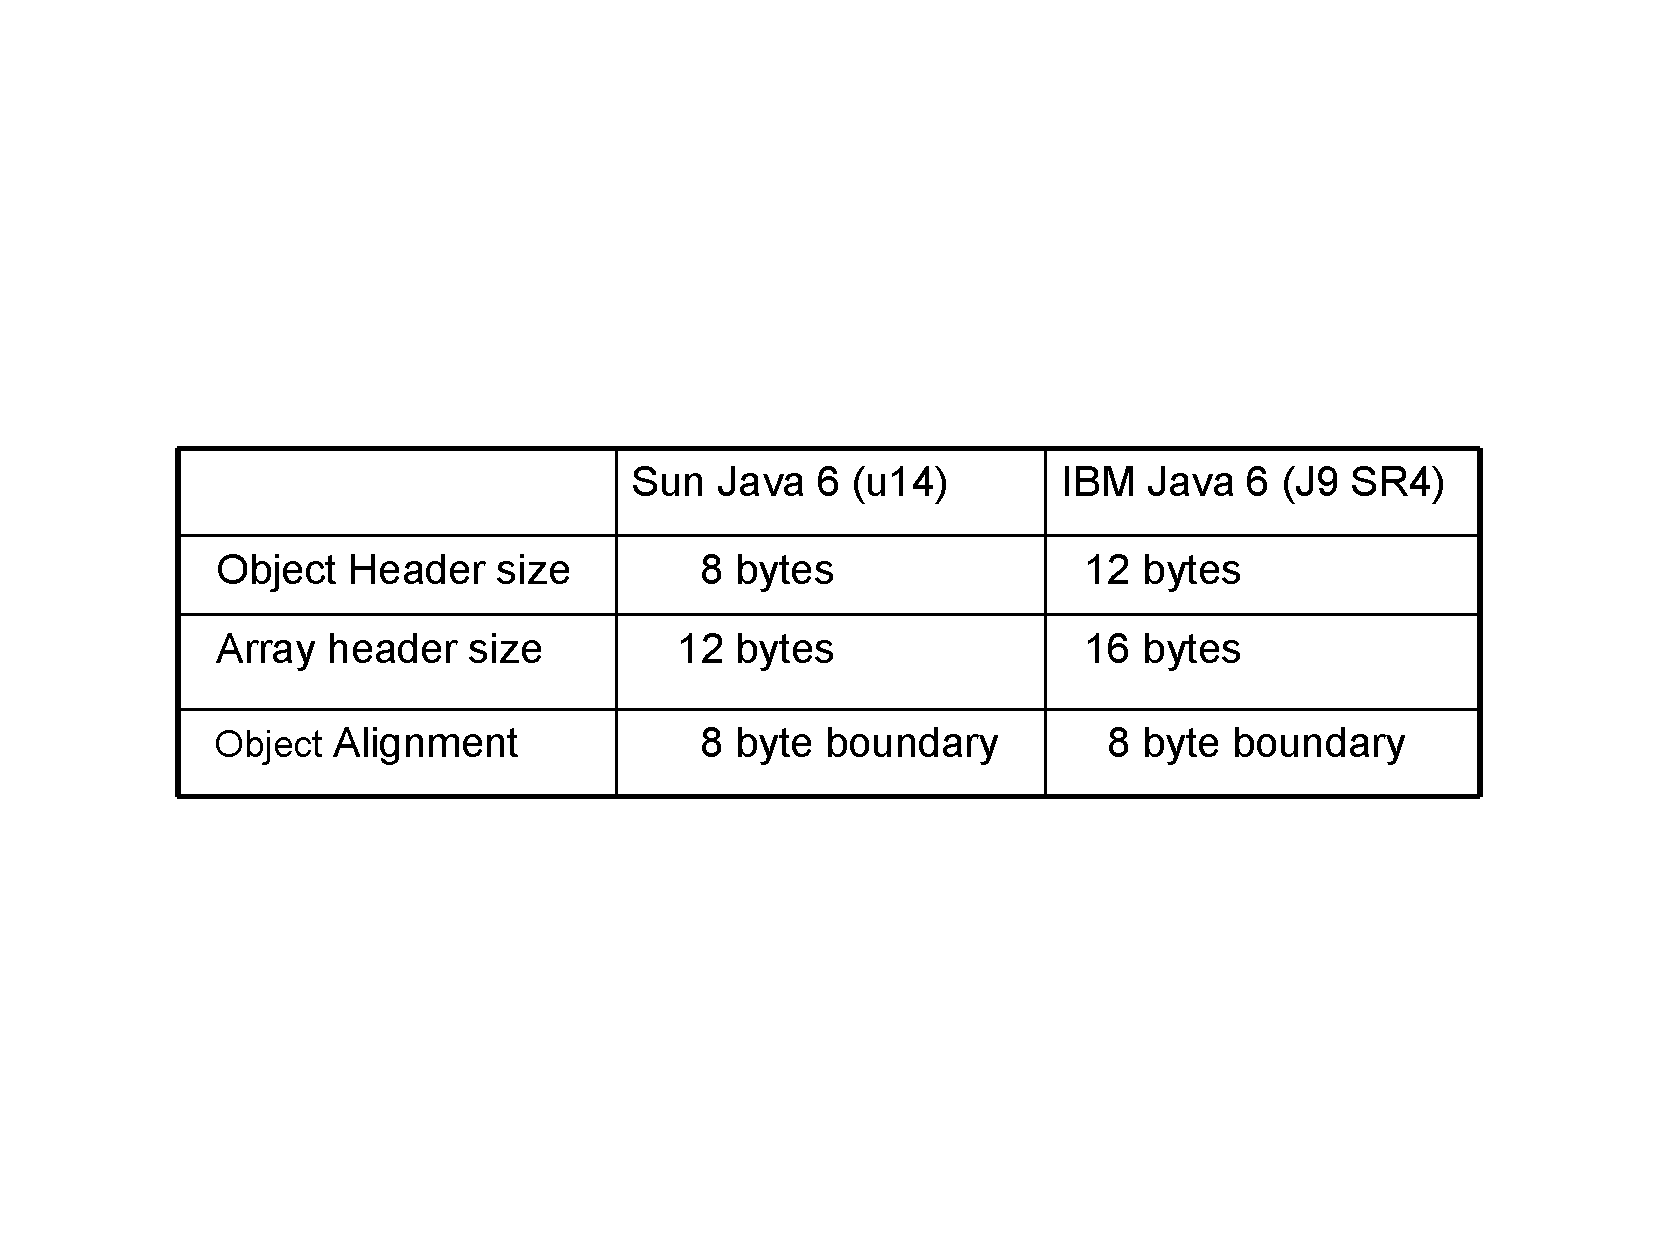
\includegraphics[width=.70\textwidth]{part1/Figures/modelingdatatypes/object-overhead.pdf}
 % \includegraphics{eight-char-string}
 \begin{tabular}{lll} \toprule
 	& Sun \javasix (u14) & IBM \javasix (SR4) \\ \midrule
 	Object header size & 8 bytes & 12 bytes \\
 	Array header size & 12 bytes & 16 bytes \\
 	Object alignment & 8 byte boundary & 8 byte boundary \\
 	Minimum field alignment & 1 byte boundary & 4 byte boundary \\
 	\bottomrule
 \end{tabular}
  \caption{Object overhead used by the Sun and IBM \jres for 32-bit architectures.}
  \label{tab:object-overhead}
\end{table} 
   %The Sun JVM allocates 8 bytes per object header, and the IBM JVM allocates 12 bytes per header. 
   
The simplest objects are the boxed scalars, which are objects with a single
primitive data type field. Since both of these \jres align objects on
8-byte boundaries and object headers are at least 8 bytes, a boxed scalar takes
at least 16 bytes. Table~\ref{tab:boxed-scalar-sizes} gives the sizes of boxed
scalars.

\begin{table}
  \centering
%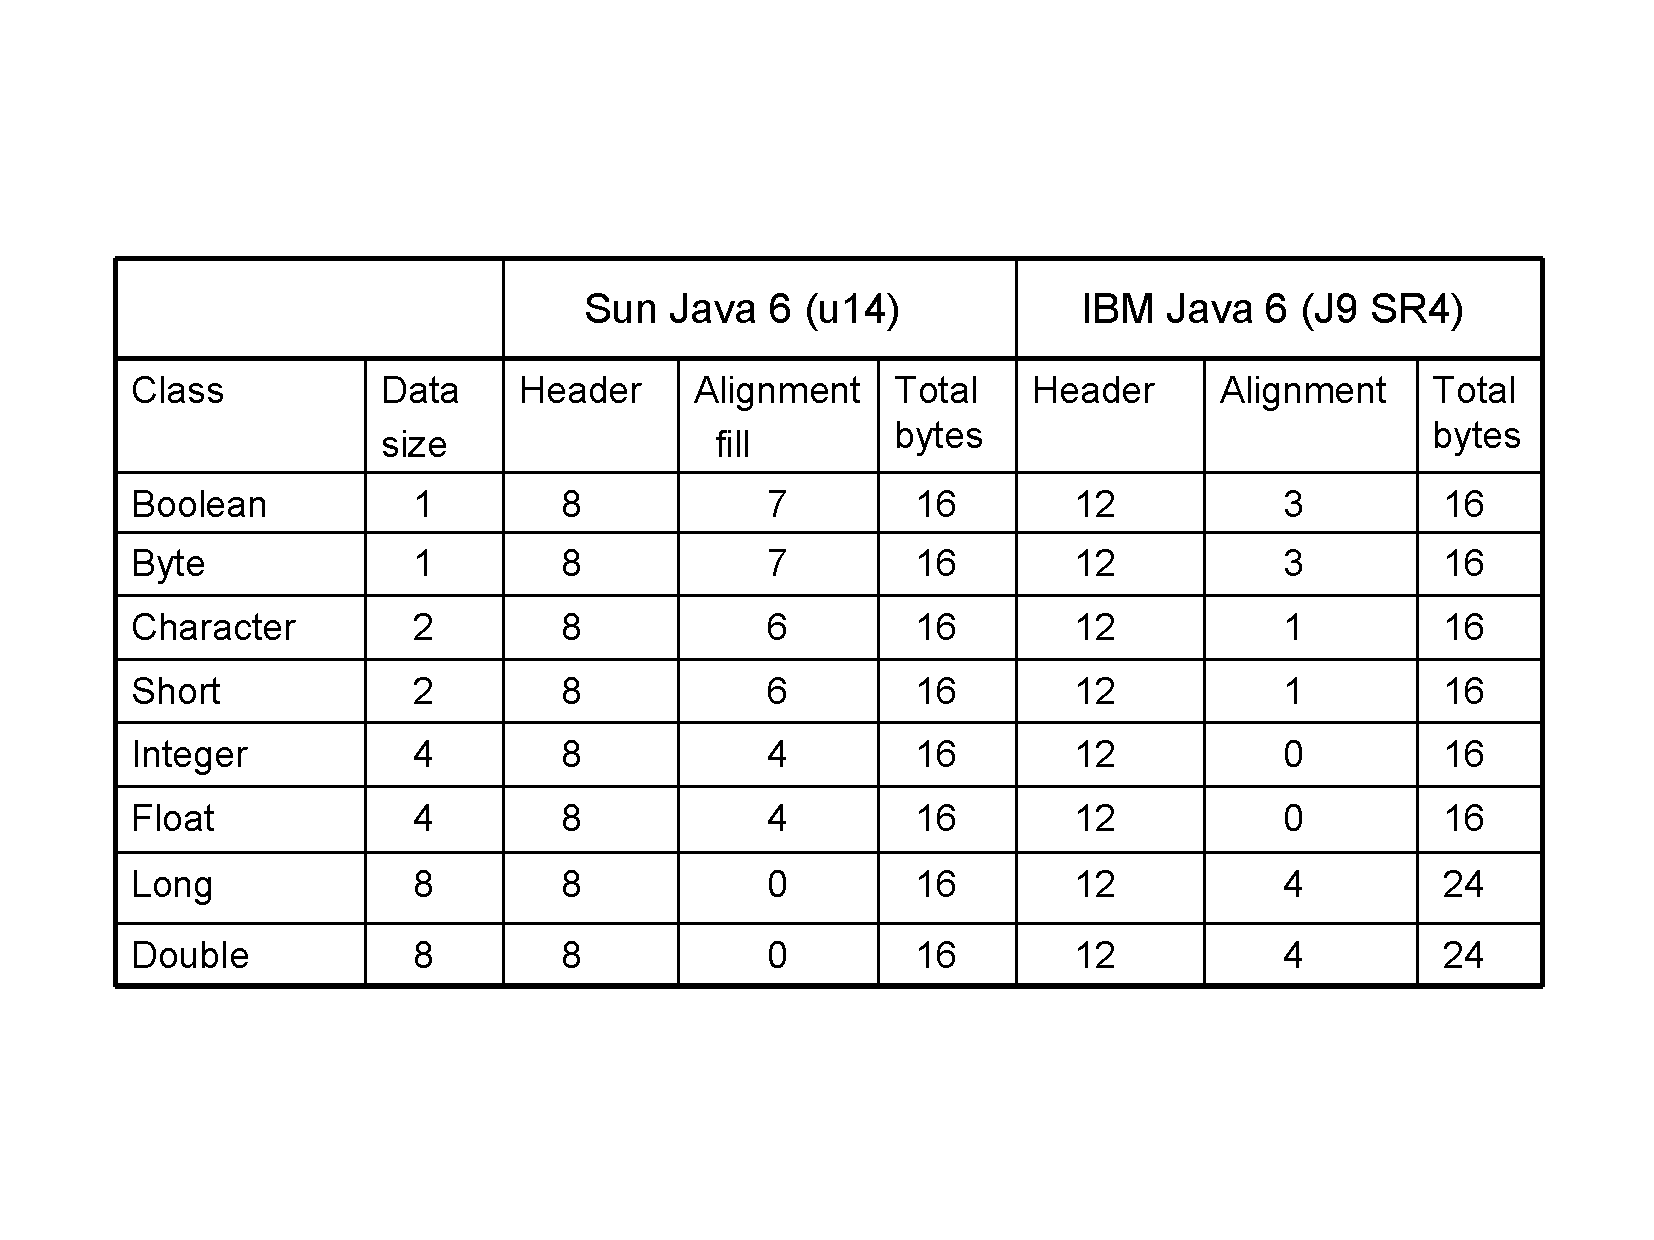
\includegraphics[width=.70\textwidth]{part1/Figures/modelingdatatypes/boxed-scalar-sizes.pdf}
	\begin{tabular}{lccccccc} \toprule
    	& & \multicolumn{3}{c}{Sun \javasix (u14)} & \multicolumn{3}{c}{IBM
    	\javasix (SR4)} \\ \cmidrule(r){3-5} \cmidrule(l){6-8}
    	%
    	Class & \shortstack[c]{Data\\size} & Header & \shortstack{Align-\\ment
    	fill} & \shortstack[c]{Total\\bytes} & Header & \shortstack{Align-\\ment
    	fill} & \shortstack[c]{Total\\bytes}
    	\\ \midrule 
    	%
    	{Boolean,} & \multirow{2}{*}{1} & \multirow{2}{*}{8} & \multirow{2}{*}{7} &
    	\multirow{2}{*}{16} & \multirow{2}{*}{12} & \multirow{2}{*}{3} &
    	\multirow{2}{*}{16}
    	\\
    	Byte & \\ \addlinespace
    	%
    	Character, & \multirow{2}{*}{2} & \multirow{2}{*}{8} & \multirow{2}{*}{6}
    	& \multirow{2}{*}{16} & \multirow{2}{*}{12} & \multirow{2}{*}{1} &
    	\multirow{2}{*}{16} \\
    	Short & \\ \addlinespace
    	%
    	Integer, & \multirow{2}{*}{4} & \multirow{2}{*}{8} & \multirow{2}{*}{4} &
    	\multirow{2}{*}{16} & \multirow{2}{*}{12} & \multirow{2}{*}{0} &
    	\multirow{2}{*}{16}
    	\\
    	Float & \\ \addlinespace
    	%
    	Long, & \multirow{2}{*}{8} & \multirow{2}{*}{8} & \multirow{2}{*}{0} &
    	\multirow{2}{*}{16} & \multirow{2}{*}{12} & \multirow{2}{*}{4} &
    	\multirow{2}{*}{24} \\
    	Double & \\
		\bottomrule
	\end{tabular}
  \caption{The sizes of boxed scalar objects, in bytes, for 32-bit
  architectures.}
  \label{tab:boxed-scalar-sizes}
\end{table}
 
\paragraph{Field-level overhead} Estimating the size of an object with more
than one field is a bit more complicated, since the hardware imposes additional
alignment requirements on specific data types. For example, integer fields are
usually aligned on 4 byte boundaries. This field alignment potentially introduces more padding.

%\begin{example}{Simple Employee Class.}
For example, consider a class \class{SimpleEmployee}, which has all primitive fields.
The comments show the number of bytes needed to store the primitive data.

\begin{shortlisting}
class SimpleEmployee {
    int id;               // 4 bytes
    int hoursPerWeek;     // 4 bytes       
    boolean exempt;       // 1 byte          
    double salary;        // 8 bytes          
    char jobCode;         // 2 bytes           
    int yearsOfService;   // 4 bytes      	
}
\end{shortlisting}
%\end{example}

If the fields are laid out one after the other with no fill, then the
field \class{salary} would have to begin on a 5-byte boundary, which is not allowed for
\class{doubles}. To avoid adding 3 more bytes of padding, the \jre could rearrange the fields
to take up the smallest amount of space. In fact, the Sun \jre does a good job rearranging and
packing fields, and the IBM \jre does not. This means that field sizes depend on the specific \jre also. 

Using the Sun \jre, you can assume each field is the size of its primitive data type because the fields are packed. The size of a
\class{SimpleEmployee} object is 32 bytes:

\begin{shortlisting}               
8 + (4+4+1+8+2+4) = 31 bytes, rounds up to 32 bytes
\end{shortlisting} 

In contrast, using the IBM \jre, all fields in non-array objects are either 4 or
8 bytes. Here is the \class{SimpleEmployee} class with field sizes adjusted
accordingly.
\begin{shortlisting} 
class SimpleEmployee {
    int id;                  // 4 bytes
    int hoursPerWeek;        // 4 bytes
    boolean exempt;          // 4 byte
    double salary;           // 8 bytes
    char jobCode;            // 4 bytes
    int yearsOfService;      // 4 bytes
}
\end{shortlisting}
The size of a \class{SimpleEmployee} is 40 bytes:
\begin{shortlisting}
12 + (4+4+4+8+4+4) = 40 bytes, with no object alignment needed
\end{shortlisting}

\paragraph{Arrays} For arrays, the data is always packed with no spaces. For
example, here is a formula that estimates the size of an array of 100 \code{chars}:
\begin{shortlisting}
header + 100*2, round up to a multiple of the object alignment
\end{shortlisting}

\callout{callout:minimum-size-estimation-rule}{Estimating Object Sizes}{
\index{Estimating Object Size}
The size of an object can be estimated as follows:
\begin{enumerate}
\item Add together the sizes of all of the fields and the object header. Fields include those in the object's class and all of its superclasses.
\item Round up the result to the next multiple of the object alignment.
\end{enumerate}
The object header size and alignment depend on the \jre.
Field sizes also depend on the \jre. For example, the \jre may pack fields to obtain the minimum
possible size, or align fields on word boundaries. Array data is always packed. }

For objects with only a small amount of primitive data, the overhead is relatively high. 
But as the amount of primitive data increases, the bloat factor decreases. 
The overhead cost consists of a fixed object header cost and a bounded alignment cost,
which are amortized when the object is big.  For example, for the Sun \jre, the bloat factors for the boxed
scalars range from 94\% for a \class{Boolean} down to 50\% for a
\class{Double}.  The bloat factor for a \class{SimpleEmployee} is 28\%.  The
bloat factor for an array of 100 \code{char}s is insignificant.  
An exception to this rule is when objects
have a lot of fields such as \code{boolean}s, that carry very little data. 
These objects will have a high bloat factor, especially if the \jre doesn't pack
fields tightly. In that case, the more fields, the more overhead.

\section{The Cost of Delegation}
\index{Delegation}

The \class{SimpleEmployee} class is not very realistic, since it has only
primitive fields. Usually, a class has some fields that are objects. In Java,
this kind of field is implemented using
\textit{delegation}, that is, by storing a reference to another object. 
%Unlike C++ and some other languages, Java does not let you embed
%one object inside another.

%\begin{example}{Employee class with delegation}
Here is a more realistic employee class with several reference fields. An
employee now has a name, which is a \class{String}, instead of an integer id. It
also has a start date, which is a \class{Date}. The type of \class{salary} has
been changed from \code{double} to \class{BigDecimal}. \class{BigDecimal} avoids potential roundoff errors.
\begin{shortlisting} 
class Employee {
    String name;                // 4 bytes
    int hoursPerWeek;           // 4 bytes
    BigDecimal salary;          // 4 bytes
    Date startDate;             // 4 bytes
    boolean exempt;             // 1 byte
    char jobCode;               // 2 bytes
    int yearsOfService;         // 4 bytes
}
\end{shortlisting}

On 32-bit architectures, a pointer is 4 bytes. 
You can calculate the size of any object as described in
Section~\ref{sec:CostOfObjects}.
% plugging in 4 bytes for each reference field.
Assuming the Sun \jre, the size of an \c{Employee} object is 32 bytes:
\begin{shortlisting}
8 + (4+4+4+4+1+2+4) = 31, rounds up to 32 bytes
\end{shortlisting}
%\end{example}

While an instance of the \class{Employee} class is a single 32
byte object, an entire employee, including name, salary, and start date
consists of five objects. Two of these objects are used to store the name.
(Recall from Section~\ref{sec:bloat-def} that a string is represented by a
wrapper \class{String} object and a \class{char} array.) The memory layout for
a specific employee ``John Doe" is shown in Figure~\ref{fig:employee-status}.
 \begin{figure}
  \centering
 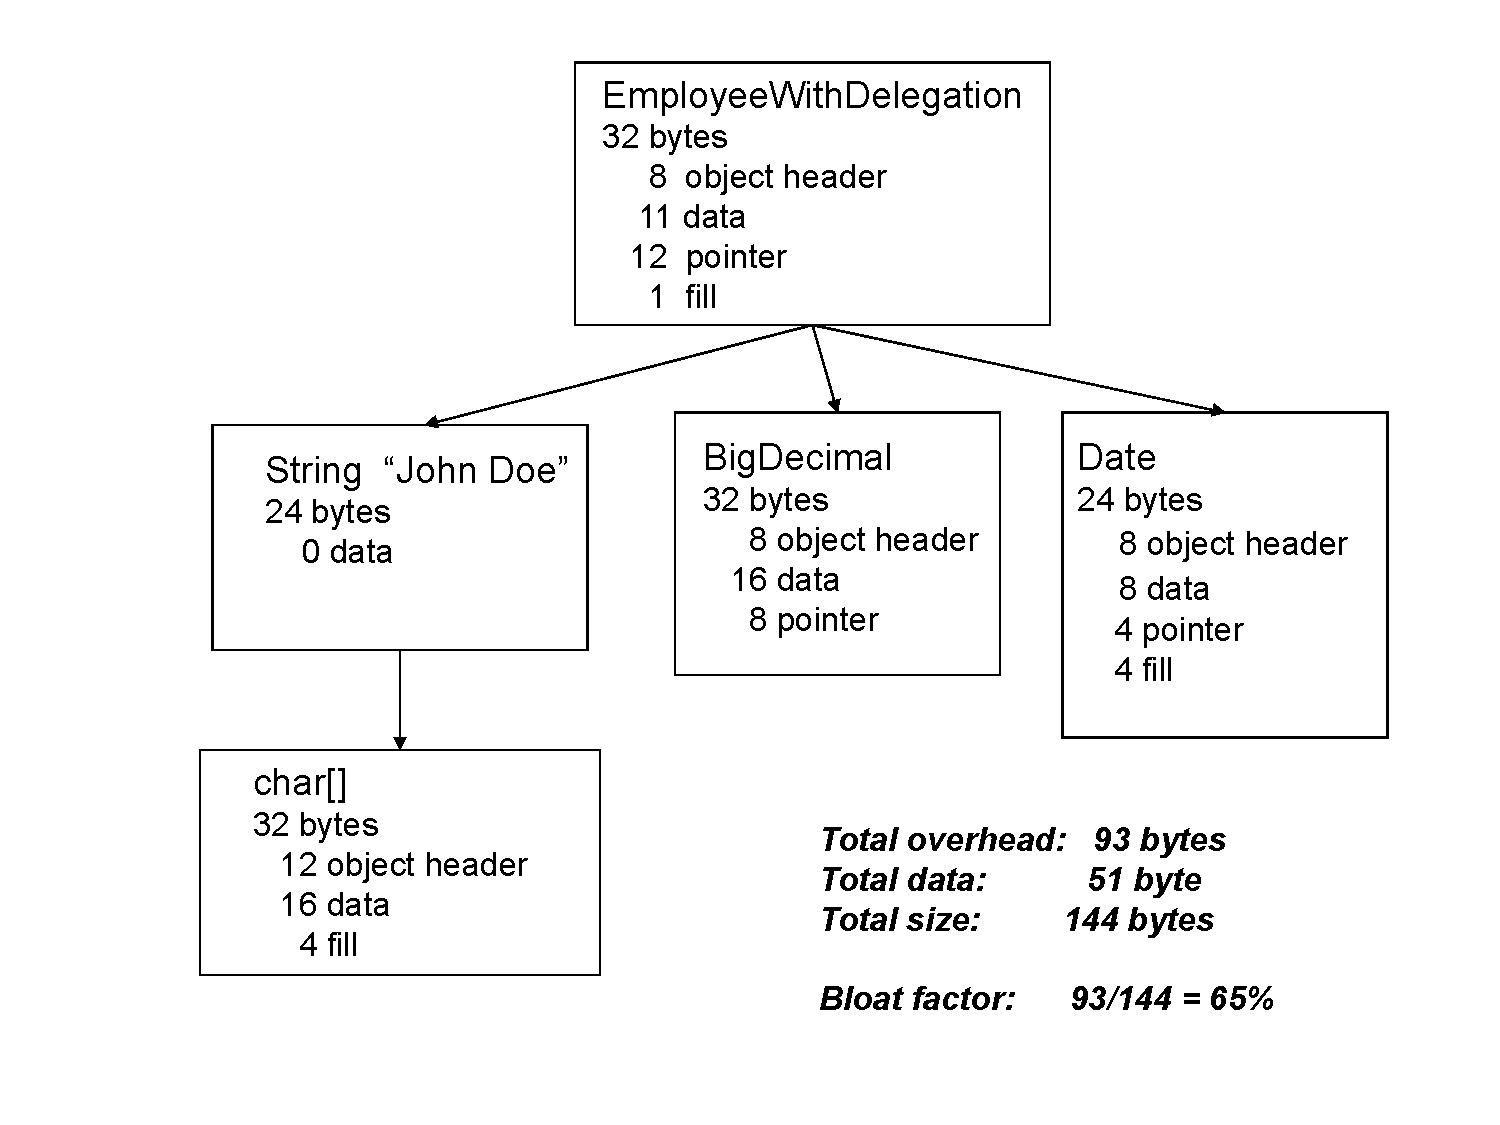
\includegraphics[width=.80\textwidth]{part1/Figures/modelingdatatypes/employee-status.pdf}
 % \includegraphics{eight-char-string}
  \caption{The memory layout for an employee, with some field data
  delegated to additional objects.}
  \label{fig:employee-status}
\end{figure}

A comparion of a \class{Employee} object with a
\class{SimpleEmployee} object from Section~\ref{sec:CostOfObjects} shows that
the size has increased from 32 to 144 bytes, and the bloat factor has increased
from 28\% to 65\%.
There is more information stored in the new version, so it is no surprise that it is bigger. The increase
in the bloat factor is more significant. Delegation increases memory bloat. Delegation introduces additional
object headers, a pointer for each delegated object, including empty
pointer slots for uninitialized object fields. Delegation may also force additional alignment costs, since
each new delegated object has to be aligned to an 8-byte boundary.

In the spirit of keeping things simple, Java does not allow you to nest objects
inside other objects, to build a single object out of other objects. You cannot
nest an array inside an object, and you cannot store objects directly in an
array.  You can only point to other objects. Even the basic data type
\class{String} consists of two objects. This means that delegation is pervasive
in Java programs, and it is difficult to avoid a high level of delegation
overhead. Single inheritance is the only language feature that can be used
instead of delegation to compose two objects, but single inheritance has limited
flexibility.  In contrast, C++ has many different ways to compose objects. C++
has single and multiple inheritance and union types. C++ allows you
to have fields that are \code{classes}, \code{structs}, or arrays, not just
references to them.  Similarly, you can have arrays of \code{class} or
\code{struct}.

Because of the design of Java, there is a basic delegation cost that is hard to eliminate.
This is the cost of object-oriented programming in Java. While it is hard to avoid this basic
delegation cost, it is important not to make things a lot worse, as discussed in the next section. 

\section{Fine-Grained Data Models}
\label{fine-grained-data-models}

The software engineering culture tends to promote delegation, and for good reasons. 
Delegation provides a loose coupling of objects, making refactoring and reuse easier. 
Replacing inheritance by delegation is often recommended, especially if the base class
has extra fields and methods that the subclass does not need. In languages with single inheritance,
once you have used up your inheritance slot, it becomes hard to refactor your code. Therefore,
delegation can be more flexible than inheritance for implementing polymorphism. However, overly fine-grained
data models can be expensive both in execution time and memory space. 

There is no simple rule that can always be applied to decide when to use delegation. Each situation has to be evaluated
in context, and there may be tradeoffs among different goals. To make an informed decision, it is important to know what
the costs are.

%\begin{example}{Employee emergency contact} 
Suppose an emergency contact is needed for each employee. An emergency contact is a person along with a preferred method
to reach her.  The preferred method can be email, cell phone, work phone, or home phone. All contact information for
the emergency contact person must be stored, just in case the preferred method does not work in an actual emergency. 
%\end{example}
Here are class definitions for an emergency contact, written in a highly delegated style that is not uncommon in real applications. 

\begin{shortlisting} 
class EmployeeWithEmergencyContact {
    ...
    EmergencyContact contact;
}
			
class EmergencyContact {
    ContactPerson contact;
    ContactMethod preferredContact;
}
			
class ContactPerson {
    String name;
    String relation;
    EmailAddress email;
    PhoneNumber phone;
    PhoneNumber cell;
    PhoneNumber work;
}
			
class ContactMethod {
    ContactPerson owner;
}
			
class PhoneNumber extends ContactMethod {
    byte[] phone;
}
			
class EmailAddress extends ContactMethod {
    String address;
}
\end{shortlisting}
 \begin{figure}
  \centering
 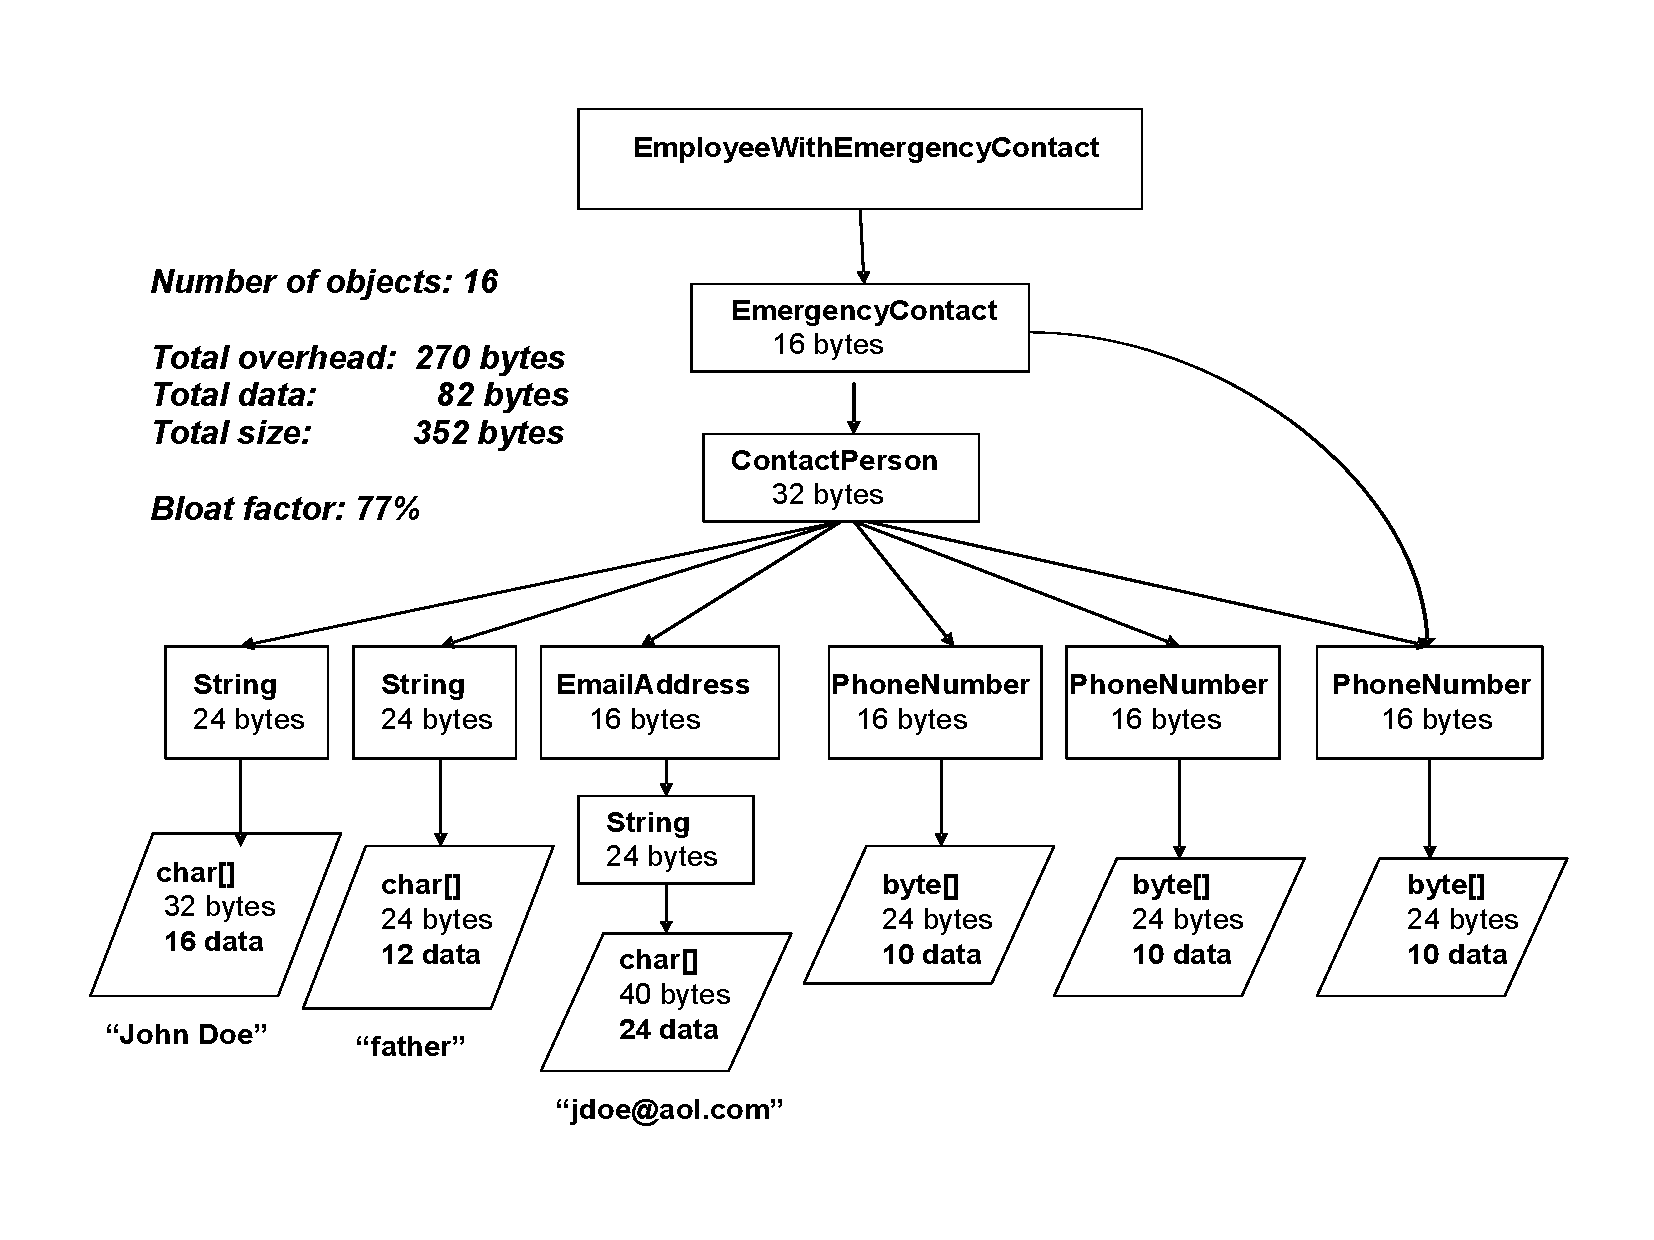
\includegraphics[width=\textwidth]{part1/Figures/modelingdatatypes/employee-status-fine-grained.pdf}
 % \includegraphics{eight-char-string}
  \caption{The memory layout for an employee with an emergency contact.}
  \label{fig:employee-status-fine-grained}
\end{figure}
The memory layout for a sample employee is shown in Figure~\ref{fig:employee-status-fine-grained}. There are 15 objects used to store emergency contact information, with a bloat factor of 77\%, which seems excessive. The objects are all small, containing only one or two meaningful fields, which is a symptom of an overly fine grained data model. Also, all of the data is at the bottom of object chains, 4 to 5 objects long. Refactoring can flatten this structure somewhat, undoing a few of the delegation.

One object that looks superfluous is \class{EmergencyContact}, which
encapsulates the contact person and the preferred contact method. Reversing
this delegation involves inlining the fields of the \class{EmergencyContact}
class into other classes, and eliminating the \class{EmergencyContact} class.
Here are the refactored classes:
\begin{shortlisting}
class EmployeeWithEmergencyContact {
    ...
    ContactPerson contact;
}
			
class ContactPerson {
    String name;
    String relation;
    EmailAddress email;
    PhoneNumber phone;
    PhoneNumber cell;
    PhoneNumber work;
    ContactMethod preferredContact;
}
\end{shortlisting}
This change eliminates an object from
Figure~\ref{fig:employee-status-fine-grained}, but it only recovers 8 bytes,
since a 16 byte object is removed and \class{ContactPerson} is 8 bytes bigger.
You can save considerably more space by inlining the four \class{ContactMethod}
classes into the \class{ContactPerson} class, which removes 64 bytes of
overhead. In a system with many instances of employees stored in memory, this
reduction is significant. In order to make this change, the preferred contact
method must be encoded somehow in \class{ContactPerson}.  A simple way to
achieve this is to use an enumeration type field, which has the same size as a reference field, to discriminate among the different contact methods:
\begin{shortlisting} 
enum PreferredContactMethod {
    EMAIL, HOME_PHONE, CELL_PHONE, WORK_PHONE;
}
      
class ContactPerson {
    PreferredContactMethod preferred;
    String name;
    String relation;
    String email;
    byte[] cellPhone;
    byte[] homePhone;
    byte[] workPhone;
}		
\end{shortlisting}
Figure~\ref{fig:refactored-fine-grain} shows the memory layout after these changes. Both the size and the bloat factor have been reduced.
 \begin{figure}
  \centering
 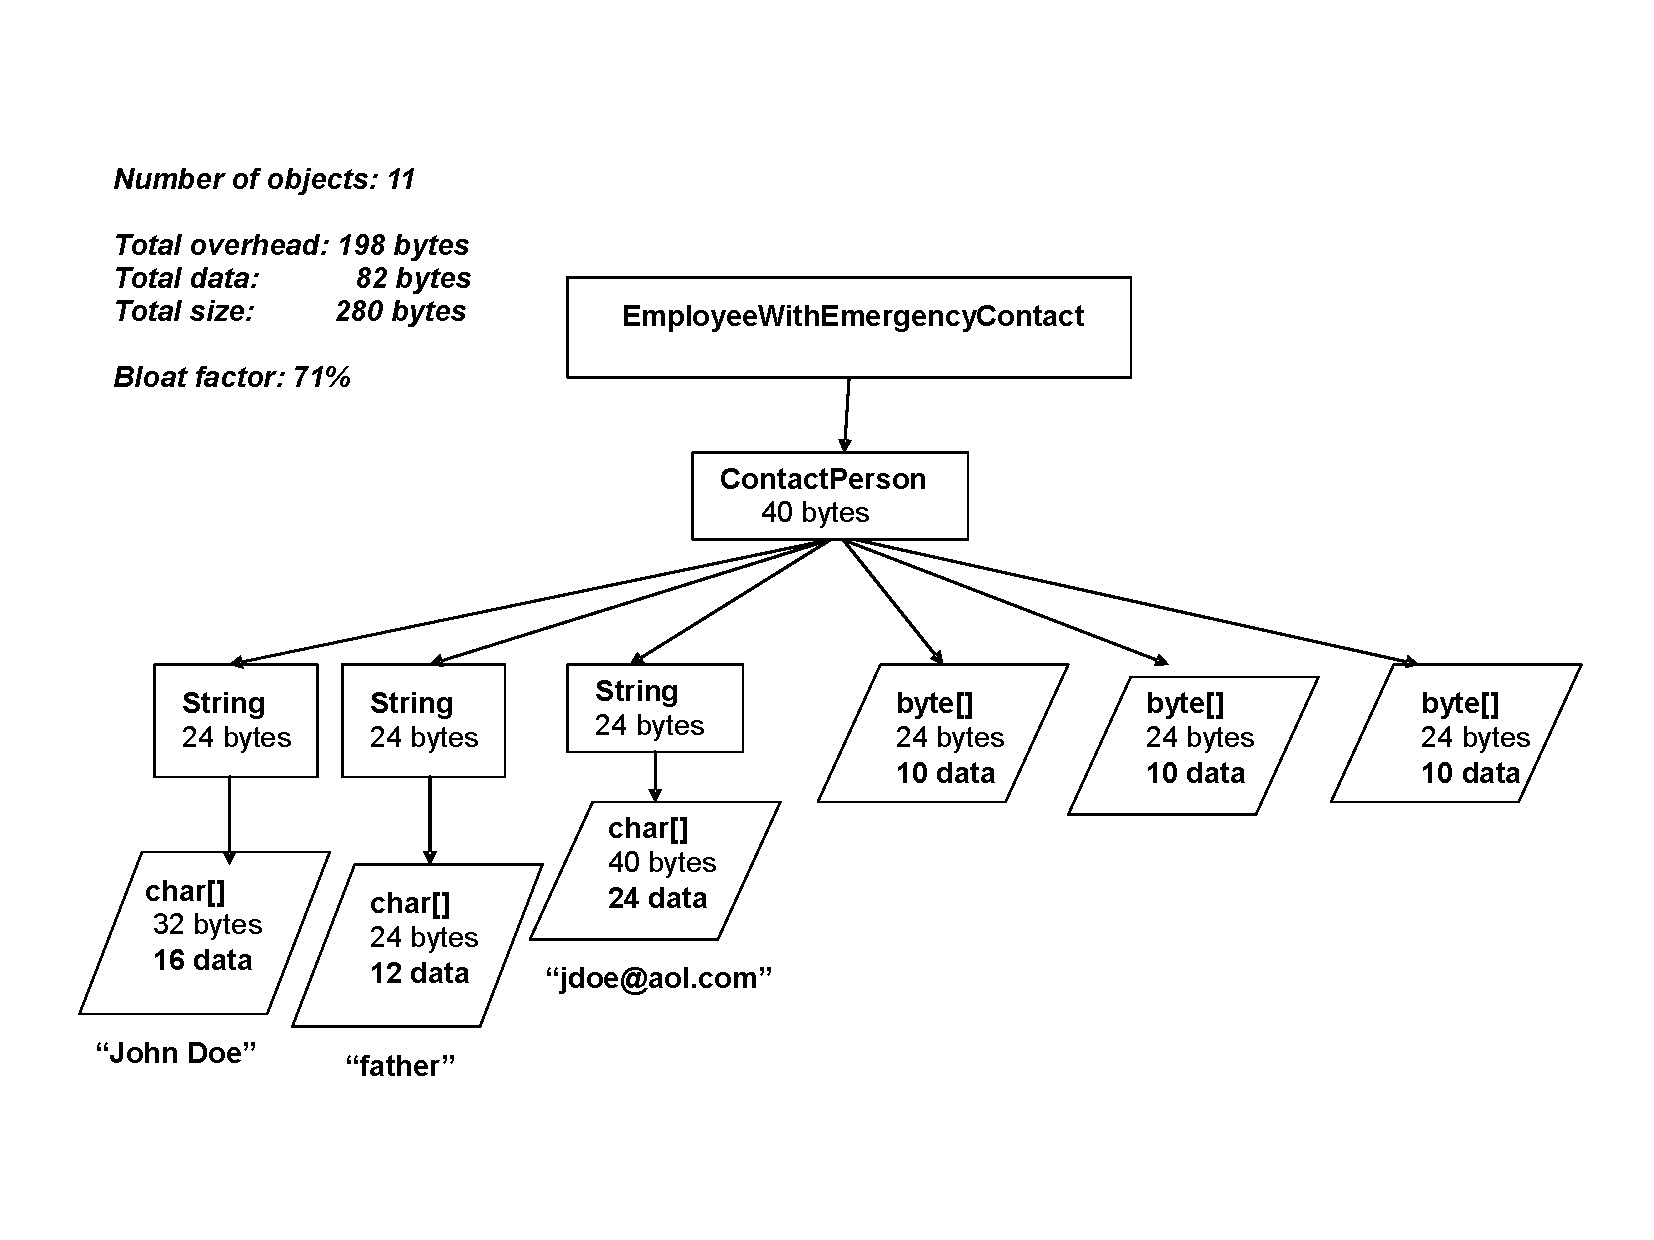
\includegraphics[width=\textwidth]{part1/Figures/modelingdatatypes/refactored-fine-grain.pdf}
 % \includegraphics{eight-char-string}
  \caption{Memory layout for refactored emergency contact.}
  \label{fig:refactored-fine-grain}
\end{figure}

When many objects are used to represent one logical concept, this is an indication that the data model may be using too much delegation. Delegation is good, but it is possible to overuse a good thing.  A design with fewer, bigger objects has less overhead and is more scalable. Whenever you use delegation, there should be a good reason. This is especially true for the important data entities in an application, those that will determine the scalability of the program.  
 

\section{64-bit Architectures}
\index{64-bit}

If your application does not fit into memory, perhaps moving to a 64-bit architecture will save you. 
However, to support a 64-bit address space, more memory is required. Object header sizes double, and pointers are
8 bytes instead of 4. Some studies~\cite{compressedAddress} show that memory consumption can increase by 40\%-50\%
going from a 32-bit to a 64-bit address space for the same Java program.

%\begin{example}{8-character string} 
Consider what happens to the 8-character string from
Section~\ref{sec:bloat-def} in a 64-bit \jre. The memory layout is shown in
Figure~\ref{fig:8-char-string-64-bit}. The 64-bit string is 50\% bigger than the 32-bit string. All of the
additional cost is overhead.
%\end{example}
 
 \begin{figure}
  \centering

 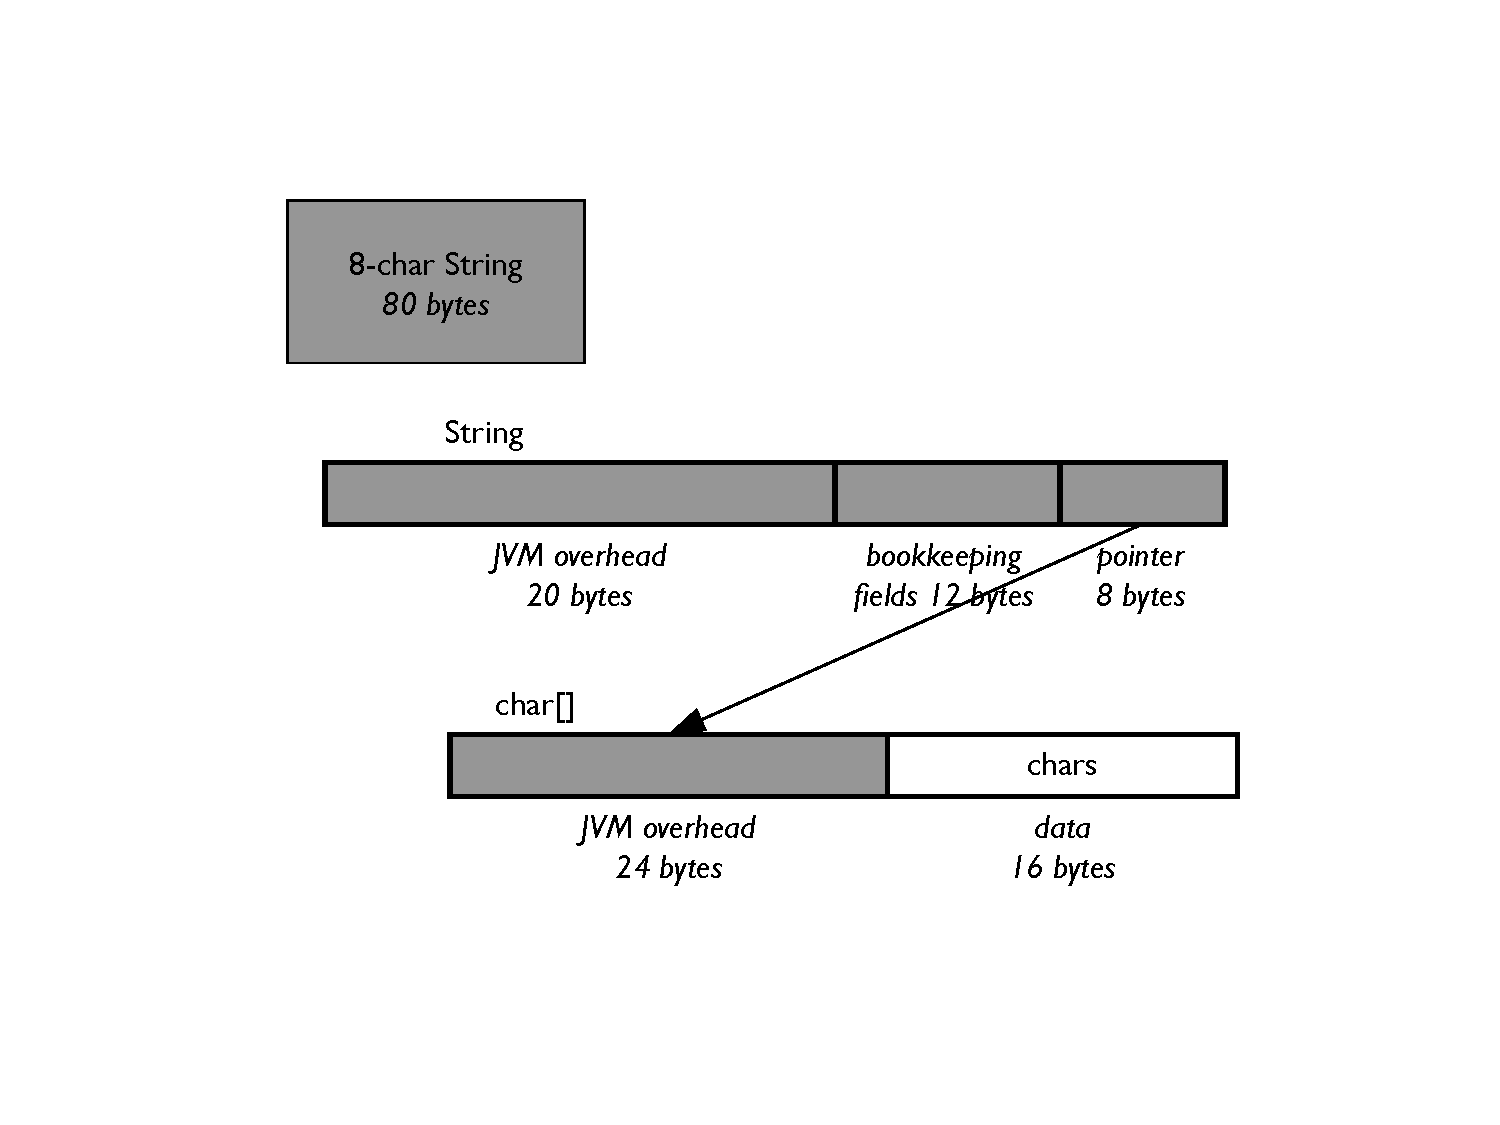
\includegraphics[width=0.8\textwidth]{part1/Figures/modelingdatatypes/8-char-string-64-bit.pdf}
 % \includegraphics{eight-char-string}
  \caption{The memory layout for an 8 character string by a 64-bit \jre.}
  \label{fig:8-char-string-64-bit}
\end{figure}

In reality, things are not so bad. Both the Sun and the IBM \jres have
implemented a scheme for compressing addresses that avoids this blowup, provided that the heap is
less than 32 gigabytes. Address compression is implemented by stealing a few unused bits from 32-bit pointers.
During execution, 32-bit compressed addresses are converted into 64-bit native addresses, and vice-versa.
See Appendix~\ref{chapter:jre-comparison} for the specifics of using this
feature.


\section{Summary}

%An entity is modeled by a set of interrelated classes. This chapter describes how to estimate the size of an instantiated entity, using rules for estimating the size of basic objects. During the modeling process, programmers choose how many classes to define.
The decision to delegate functionality to another object sometimes involves making a tradeoff between flexibility and memory cost. You need to decide how much flexibility is really needed, and you also need to be aware of the actual memory costs. This chapter provides the basic knowledge for estimating memory costs. 
\begin{itemize}
\item An object size depends on the object header size, field alignment, object
alignment, and pointer size. These can vary, depending on the \jre and the
hardware. The size of an object is the sum of the header and the field
sizes, rounded up to an alignment boundary. 
\end{itemize}
If you need the exact size of objects, there are various tools available. A list of resources is provided in the Appendix.

This chapter also describes several costly anti-patterns to avoid.
\begin{itemize}
\item A \textit{highly-delegated data model} results in too many small objects and a large bloat factor. Typically, each object has only a few fields, which is excessive data granularity.  
\item A \textit{highly-delegated data model with large base classes} results in too many big objects. Often, the data model is providing a fine granularity of function, which may no be needed.
\end{itemize}   

Both the design of Java and software engineering best practices encourage highly delegated data models with many objects. This cost is often considered to be insignificant --- delegating to another object is just a single level of indirection. But the costs of the pointers and object headers needed to implement delegation indirection add up quickly, and contribute significantly to large bloat factors in real applications. 

  


\chapter{Field Patterns for Efficient Objects}
\label{chapter:field-patterns}

[TODO: Fix word wrap in source listings]

In many applications, the heap is filled mostly with instances of just a
few important classes.  You can increase scalability significantly by making these
objects as compact as possible. This chapter describes field usage
patterns that can be easily optimized for space, for example, fields that are
rarely needed, constant fields, and dependent fields. Simple refactoring of
these kinds of fields can sometimes result in big wins.
 

\section{Rarely Used Fields}
\label{sec:rarely-used}

\paragraph{Side Objects}Chapter~\ref{chapter:delegation} presents examples
where delegating fields to another class increases memory cost. However, sometimes delegation can
actually save memory, if you don't have to allocate the delegated object all the
time.

As an example, consider an on-line store with millions of products. 
Most of the products are supplied by the parent company, but
sometimes the store sells products from another company:
\begin{shortlisting} 
class Product {
	String sku;
	String name;
	..
	String alternateSupplierName;
	String alternateSupplierAddress;
	String alternateSupplierSku;
}
\end{shortlisting}
When there is no alternate supplier, the last three fields
are never used. By moving these fields to a separate side class, you can
 save memory, provided the side object is allocated only when
it is actually needed. This is called \emph{lazy allocation}. Here are the 
refactored classes:

\begin{shortlisting} 
class Product {
	String sku;
	String name;
	.. 
	Supplier alternateSupplier;
}

class Supplier {
	String supplierName;
	String supplierAddress;
	String sku;
}
\end{shortlisting}
For products with no alternate supplier, eight bytes are saved per product,
since three fields are replaced by one. Of course, products with an alternate
supplier pay a delegation cost: an extra pointer and object header, totaling 12
bytes. An interesting question is how
much total memory is actually saved? The answer depends on the percentage of products that have an alternate supplier and
need
a side object, which we'll call the \emph{fill rate}. The higher the fill rate, the less memory is 
saved. In fact, if the fill rate is too high, memory is wasted.

Figure~\ref{fig:fill-rate} shows the memory saved for
different fill rates, assuming three fields (12 bytes) are delegated. The most memory that can be
saved is 8 bytes per object on average, when the fill rate is 0\%. That's 67\%
of the size of the fields that were delegated.
When the fill rate is 10\%, only 50\% of the delegated field bytes are saved on
average. When the fill rate is over 40\%, the memory saved is
negative, that is, memory is wasted. The lesson here is that if you aren't sure
what the fill rate is, then using delegation to save memory may end up
backfiring.
\begin{figure}
  \centering
 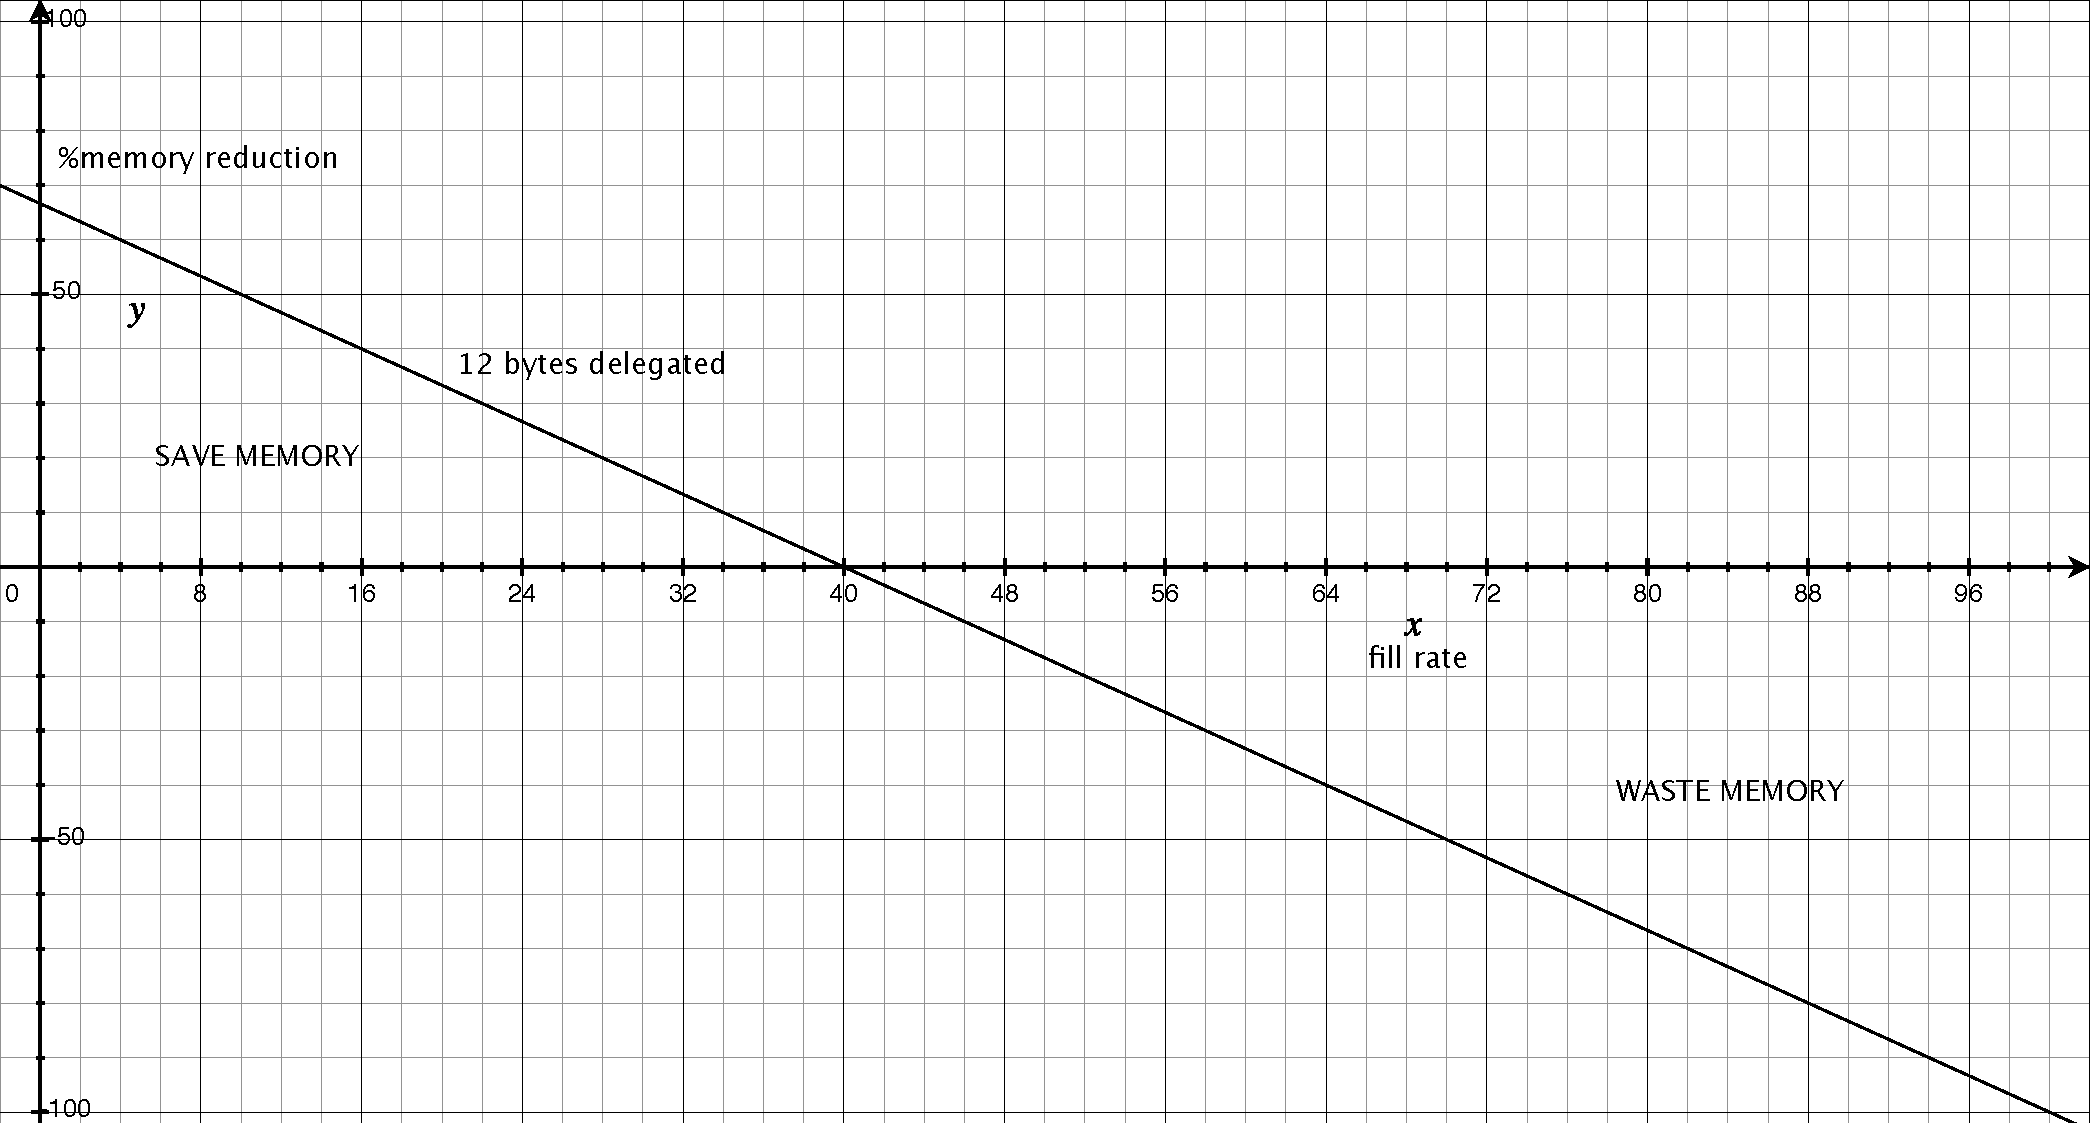
\includegraphics[width=.90\textwidth]{part1/Figures/modelingdatatypes/12-byte-graph.pdf}
 % \includegraphics{eight-char-string}
  \caption{This plot shows how much memory is saved or wasted by delegating 12
  bytes of memory to a side object. The x-axis is the fill rate, and the
  y-axis is the average memory saved as a percent of the bytes delegated.}
  \label{fig:fill-rate}
\end{figure}


In addition to the fill rate, the memory savings also depends on the
number of fields delegated and their sizes. The more bytes
delegated, the larger the memory savings, assuming the same fill rate. Figure~\ref{fig:rarely-used} shows the memory
saved or wasted for different fill rates and delegated-field sizes.
Each line represents a different delegated-field size. The bottom-most line
represents a delegated field size of 16 bytes, the next line represents 32 bytes, the next
represents 48 bytes, and so on, up to 144 bytes. As the delegated object size
increases, you can worry less about the fill rate. For example, if 32 bytes
are delegated, there is almost 90\% savings with a low fill rate, and some
memory savings with a fill rate up to 70\%. As the delegation size increases, 
the lines start to converge, since the delegation overhead becomes
less important. At larger sizes there is less of a chance
that underestimating the fill rate will cause you to waste memory, and if it
does, the memory lost will be relatively small.

\begin{figure}
  \centering
 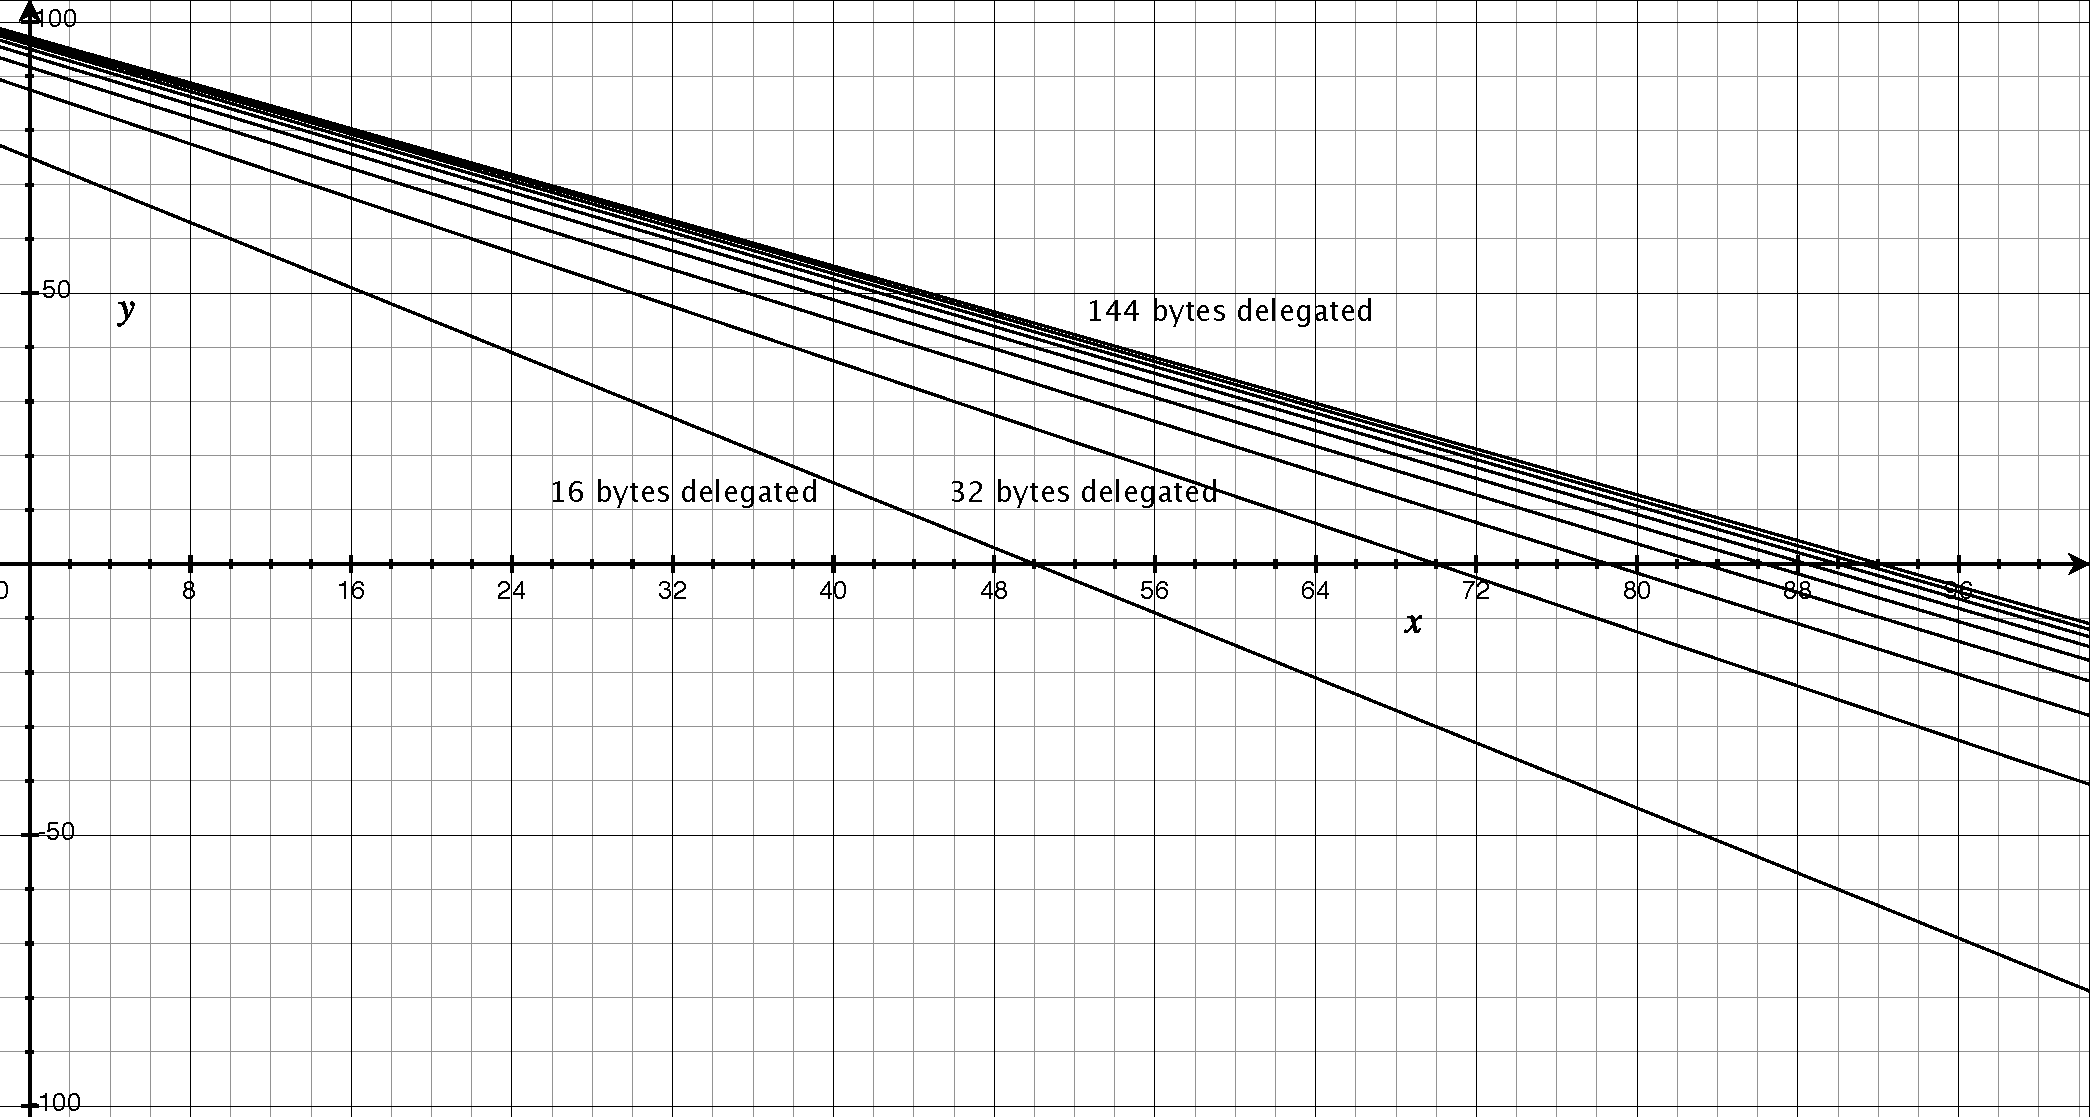
\includegraphics[width=.90\textwidth]{part1/Figures/modelingdatatypes/rarely-used.pdf}
 % \includegraphics{eight-char-string}
  \caption{This plot shows how much memory is saved or wasted
  depending on how many bytes are delegated to a side object.
  The x-axis is the fill rate, and the y-axis is the average
  memory saved as a percent of the bytes delegated. Each line represents
  a different delegated-fields size, from 16 to 144 bytes, in increments of
  16 bytes.}
  \label{fig:rarely-used}
\end{figure}

\callout{callout:rarely-used}{Delegation Savings Calculation}{
\index{Delegation Savings Calculation}
Assume the cost of a pointer is 4 bytes, and the cost of an object header is 8
bytes.  Let:
\begin{eqnarray} 
B &=& the\ size\ in\ bytes\ of\ the\ delegated\ fields \nonumber \\
F &=& the\ fill\ rate,\ between\ 0\ and\ 1 \nonumber
\end{eqnarray}

While every object pays a
4-byte pointer cost, only F of them pay for a side object. Therefore, using 
a side object will result in an average savings per object of:
\begin{eqnarray}
B-4\ \ -\ \ F(B+8) \nonumber
\end{eqnarray}

For the savings to be positive, the following must be true
\footnote{This calculation does not include alignment overhead.
Delegating fields to a side object may increase alignment costs,
depending on the other fields in your object.
If the header size is not a multiple of the alignment (e.g.
on the IBM 32-bit JRE), delegation can sometimes reduce alignment costs.}:
\begin{eqnarray}
F &<& \frac{B-4}{B+8} \nonumber
\end{eqnarray}

} 
A common error is to put rarely used fields in a side
class with lazy allocation, but have code paths that
cause the side object to be allocated all the time, even when it's not needed.
In this case, instead of saving memory, you pay the full cost of delegation as well as 
the cost of unused fields. 
Lazy allocation
can also be error-prone because it may require testing whether the object
exists at every use. If you need concurrent access to the data in the side
object, you have to take special care to code the checks correctly to avoid race
conditions.
This complexity has to be weighed against potential memory savings.

\paragraph{Side Tables}If a field is very rarely used, then it
might make sense to delete it from its class altogether, and store it in a separate table that maps
objects to attribute values. For example, suppose that only a few of the
products have won major awards, and you want to record this information. Rather than maintaining a field
\code{majorAward} in every product, you can define a table that maps a product
\code{sku} to an award.

\begin{shortlisting}
class Product {
    static HashMap<String, String> majorAward = 
    	new HashMap<String, String>();
    ..
}
\end{shortlisting}

Even though a \class{HashMap} has its own high overhead, this
design can come out ahead if there are a small number of major awards.
You can do a similar analysis as you would for side objects to decide if this
approach is worth it.
A hash entry typically takes more memory than a side object (see
Section~\ref{sec:}).
Therefore, a side table will start wasting
memory at a lower fill rate than would a side object approach.
Whenever you add a new table like this you also have to be careful not to
introduce a memory leak. If products are no longer needed and are garbage
collected, the corresponding entries in the table must be cleaned up.
This topic is discussed at length in Section~\ref{}.

\paragraph{Subclassing} The least expensive way to model rarely used fields
is to move them to a subclass. Unlike the optimizations we've discussed,
subclassing costs no extra space. It can have
some disadvantages from a software engineering standpoint, though, when compared with
delegation or a side table approach. It can make your code less flexible, making
it more difficult to add or rearrange functionality later on. Since Java
supports only single inheritance, defining a subclass for rarely used
fields will prevent you from having subclasses for
other purposes. Using delegation or a side table also allows your data to be more dynamic. 
Rarely used fields can be added after an instance is
created.
 

\section{Mutually Exclusive Fields}
\label{sec:mutually-exclusive}

Sometimes a class has fields that are never used at the same time, and therefore
they can share the same space. Two mutually exclusive fields can be conflated
into one field if they have the same type. Unfortunately, Java does not have
anything like a union type to combine fields of different types. However, if it
makes sense, mutually exclusive field types can be broadened to a common base type
to allow this optimization.

For example, suppose that each women's clothing product has a size, and there
are different kinds of sizes: xsmall-small-medium-large-xlarge,
numeric sizes, petite sizes, and large women's sizes. One way
to implement this is to introduce a field for each kind of size:
\begin{shortlisting}
class WomensClothing extends Product {
	..
	SMLSize      smlSize;
	NumericSize  numSize;
	PetiteSize   petiteSize;
	WomensSize   womensSize; 
}
\end{shortlisting}
Each type is an enum class, such as:
\begin{shortlisting}
enum SMLSize {
	XSMALL, SMALL, MEDIUM, LARGE, XLARGE;
}

enum NumericSize {
	ZERO, TWO, FOUR, SIX, EIGHT, TEN, TWELVE, FOURTEEN, SIXTEEN;
}

enum PetiteSize {
    ZERO, TWO, FOUR, SIX, EIGHT, TEN, TWELVE, FOURTEEN, SIXTEEN;
}

enum WomensSize {
	ONEX, TWOX, THREEX, FOURX;
}
\end{shortlisting}
These four size fields are mutually exclusive --- a clothing item cannot
have both a petite size and a women's size, for example. Therefore, you can
replace these fields by one field, provided that the four enum types are
combined into one enum type:
\begin{shortlisting}
enum ClothingSize {
	XSMALL, SMALL, MEDIUM, LARGE, XLARGE, 
	ZERO, TWO, FOUR, SIX, EIGHT, TEN, TWELVE, FOURTEEN, SIXTEEN,
    PETITE_ZERO, PETITE_TWO, PETITE_FOUR, PETITE_SIX, PETITE_EIGHT, PETITE_TEN,
    PETITE_TWELVE, PETITE_FOURTEEN, PETITE_SIXTEEN,
	ONEX, TWOX, THREEX, FOURX;
}

class Clothing extends Product {
	..
	private ClothingSize     size; 
	..
	public SMLSize getSMLSize() {..}
	public void setSMLSize(SMLSize smlSize) {..}

	public NumericSize getNumericSize() {..}
	public void setNumericSize(NumericSize numericSize) {..}

	public PetiteSize getPetiteSize() {..}
	public void setPetiteSize(PetiteSize PetiteSize) {..}

	public void setNumericSize(WomensSize womensSize) {..}
	public WomensSize getWomensSize() {..}
	..
} 


\end{shortlisting}

You can easily write access and update methods that translate to and from the
original types, so that the caller is insulated from this storage trick.

If the mutually exclusive fields are of different classes,
you can generalize their types by defining a common superclass, if possible.
As a last resort, you can always combine these fields into a single field of type
\class{Object}. Finally, if there are sets of fields that are mutually exclusive, then you can
define a side class for each set of fields, where all side classes have
a common superclass. In this case, you need to do the math to make sure that you
actually save memory, given the extra cost of delegation.

Just like rarely used fields, mutually
exclusive fields can also be modeled using subclassing. Again, the space savings
have to be weighed against other software engineering goals.

\section{Constant Fields}
\label{sec:constant}

Declaring a constant field \code{static} is a simple way to
save memory. Programmers usually remember to make constants like \emph{pi} 
static. There are other situations that are a bit more subtle, for example,
when a field is constant because of how it is used in the context of an
application.

Returning to the product example, suppose that each product has a field
\code{catalog} that points to a store catalog.
If you know that there is always just one store catalog, then the field
\code{catalog} can be turned into a static, saving 4 bytes per product.

As a more elaborate example, suppose that a \class{Product} has a field
referencing a \class{Category} object, where a category may be
books, music, clothes, toys, etc.
Clearly, different products belong to different categories.
However, suppose we define
subclasses \class{Book}, \class{Music}, and \class{Clothing} of the class
\class{Product}, and all instances of a subclass belong to the same category.  
Now the \code{category} field has the same value for products in each subclass,
so it can be declared static:

\begin{shortlisting}
public abstract class Product {
	public abstract Category getCategory();
	..
}

class Book extends Product {
	static Category bookCategory; // Points to the 
                                  // book category object
	public Category getCategory() {return bookCategory;}  
	..
}

class Music extends Product {
	static Category musicCategory; // Points to the
                                   // music category object
	public Category getCategory() {return musicCategory;}  
	..
}

class Clothing extends Product {
	static Category clothingCategory; // Points to the
	                                  // clothing category
                                      // object
	public Category getCategory() {return clothingCategory;}  
	.. 
}

\end{shortlisting}

Knowing the context of how objects are created and used, and how they relate to
other objects, is helpful in making these kinds of memory optimizations.

\section{Nonstatic Member Classes}
Sometimes it is useful to define a class
within a larger class or method. Java lets you create four kinds of
nested classes, each for a different purpose. They are \emph{static member},
\emph{nonstatic member}, \emph{local}, and \emph{anonymous} classes.
Instances of the latter three are always created within the
context of an instance of the enclosing class. Their methods can refer back to
the enclosing instance. To accomplish this, these three kinds of nested classes 
maintain an extra, hidden field, the \code{this} pointer of the enclosing
instance. In contrast, instances of a static member class do not have this extra
field. They are created independently of any instances of the enclosing class.

A common error is to declare a nonstatic member class 
when you don't really need to maintain a link with an
enclosing instance. To illustrate, let's return to the example from Section~\ref{sec:rarely-used},
where we moved some rarely used fields into a side class, \code{Supplier}. 
Suppose we wanted to hide this decision, so that we would have the freedom to change our
minds later if the optimization didn't work out. We could make \code{Supplier} a
member class of Product, as follows:

\begin{shortlisting}
class Product {
	class Supplier {
		String supplierName;
		String supplierAddress;
		String sku;
	}
	
	..
	Supplier alternateSupplier;
	..
	public void setAlternateSupplierName(String name) {
		// Lazily allocate the alternate supplier object
		if (alternateSupplier == null) {
			alternateSupplier = new Supplier();
		}
		alternateSupplier.supplierName = name;
	}
	..
}
\end{shortlisting}

Since we didn't declare \code{Supplier} to be static, every instance of
\code{Supplier} will contain an extra pointer back to the product which created
it. In cases like this, a static member class can work just as well, and save
the 4-byte pointer field. The only code change is to add the keyword
\code{static} to the declaration of \code{Supplier}.
Notice how Java makes it easy to make this mistake, since the \code{new}
statement that creates an instance of \code{Supplier} looks the same either way.
In the nonstatic case, it hides the fact that it's passing in the enclosing
\code{this} pointer.

The book Effective Java \cite{EffectiveJavaBook} gives the same advice,
to ``favor static member classes over nonstatic'' when you don't need to
maintain a link to the outer instance. It lists more benefits in addition
to the space savings.
For example, the hidden pointer can lead to a memory leak, by
inadvertently holding on to the enclosing instance longer than it's needed. 


\section{Redundant Fields}

A field is redundant if it can be computed on the fly from other fields, and, in
principle, can be eliminated. In the simplest case, two fields store the same
information but in different forms, since the two fields are used for
different purposes. For example, product IDs are
more efficiently compared as \code{ints}, but more easily printed as
\code{Strings}. Since it is possible to convert one representation into the
other, storing both forms is not necessary, and only makes sense if
there is a large performance penalty from performing the data
conversion.
In the more general case, a field may depend on many other values. For example,
you could allocate a field to store the number of items in a shopping cart,
 or simply compute it by adding up all of the shopping cart items. 

There is a trade-off between the performance cost of a conversion or computation
and the memory cost of an extra field, which has to be weighed in context. 
How often is the information needed and how expensive is it to compute? What's
the total memory cost? Comparing performance cost to memory cost is a bit like apples and oranges, 
but often it is clear which resource is most constrained. Here are several
considerations to keep in mind:
\begin{itemize}
  \item Computed \class{String} fields should be used only if there's a good
  reason, since strings have a very high overhead in Java, 
as we have seen.  
\item Computed fields are very useful when storing partial values avoids 
expensive quadratic computations. For example, if you need to support finding
the number of children of nodes in a graph, then caching
this value for each node is a good idea. 
\end{itemize}

If you do need to store a computed field, make sure that you are
using the most efficient representation.  For example,
\class{StringBuffer} is useful for building a character string, but is
less space-efficient than \class{String} for storing the final result.
Chapter~\ref{chapter:representing-values} compares different ways to represent some common
datatypes.
Another thing to watch for is storing many copies of the same computed
value. Even something as simple as storing a large number of empty
\class{String}s can really add up in Java.
Chapter~\ref{chapter:sharing-immutable-data} looks at ways to share
read-only data.

\section{Large Base Classes and Fine-grained Designs}
\index{Base Class Baggage}

As discussed in the previous chapter, highly-delegated data models can result in
too many small objects. Occasionally, you run across a highly-delegated data model where the delegated objects
are large. This can happen when delegated classes inherit from a large base class. When fine grained data modeling
is combined with inheriting from large base classes, memory costs multiply and can become prohibitive.

%\begin{example}{Keeping track of updates} 
A frequent data management requirement is to track creation and update information, that is, when data is created or updated and by whom.  Here is a base class, taken from a real application, that stores create and update information.  
\begin{shortlisting}
class UpdateInfo {
     Date creationDate;
     Party enteredBy;
     Date updateDate;
     Party updatedBy;
}
\end{shortlisting}
You can track changes by subclassing from \class{UpdateInfo}. Update tracking is
a \textit{cross-cutting feature}, since it can apply to any class in a data model.
%\end{example}

Returning to the original, unoptimized
version of \class{EmployeeWithEmergencyContact} in
Section~\ref{fine-grained-data-models}, suppose that updates to employee emergency contacts need to be tracked. 
You need to decide how fine the tracking should be. Should every update to every
phone number and email address be tracked, or is it sufficient to track the fact that some
contact information was changed for an emergency contact? If you decide to
track changes to every contact phone number or email address, you can easily achieve this by
extending the \class{ContactMethod} class defined in the fine-grained data model from Section~\ref{fine-grained-data-models}:
\begin{shortlisting}
class ContactMethod extends UpdateInfo {
     ContactPerson owner;
}
\end{shortlisting}
Figure~\ref{fig:big-base-class} shows an instance of a contact person with
update information associated with every \class{ContactMethod}. Not only is this
a highly delegated structure with multiple \class{ContactMethod} objects, but
each one has an additional 16 bytes. Furthermore, there are potentially four
more objects of type \class{Date} and \class{Party} for each of the four
\class{ContactMethod} objects. A far more scalable solution is to move up a
level, and track changes to each \class{ContactPerson}. With this solution, you
do not need such a fine-grained data model, and the update tracking functionality is 1/4 the cost.
\begin{figure}
  \centering
 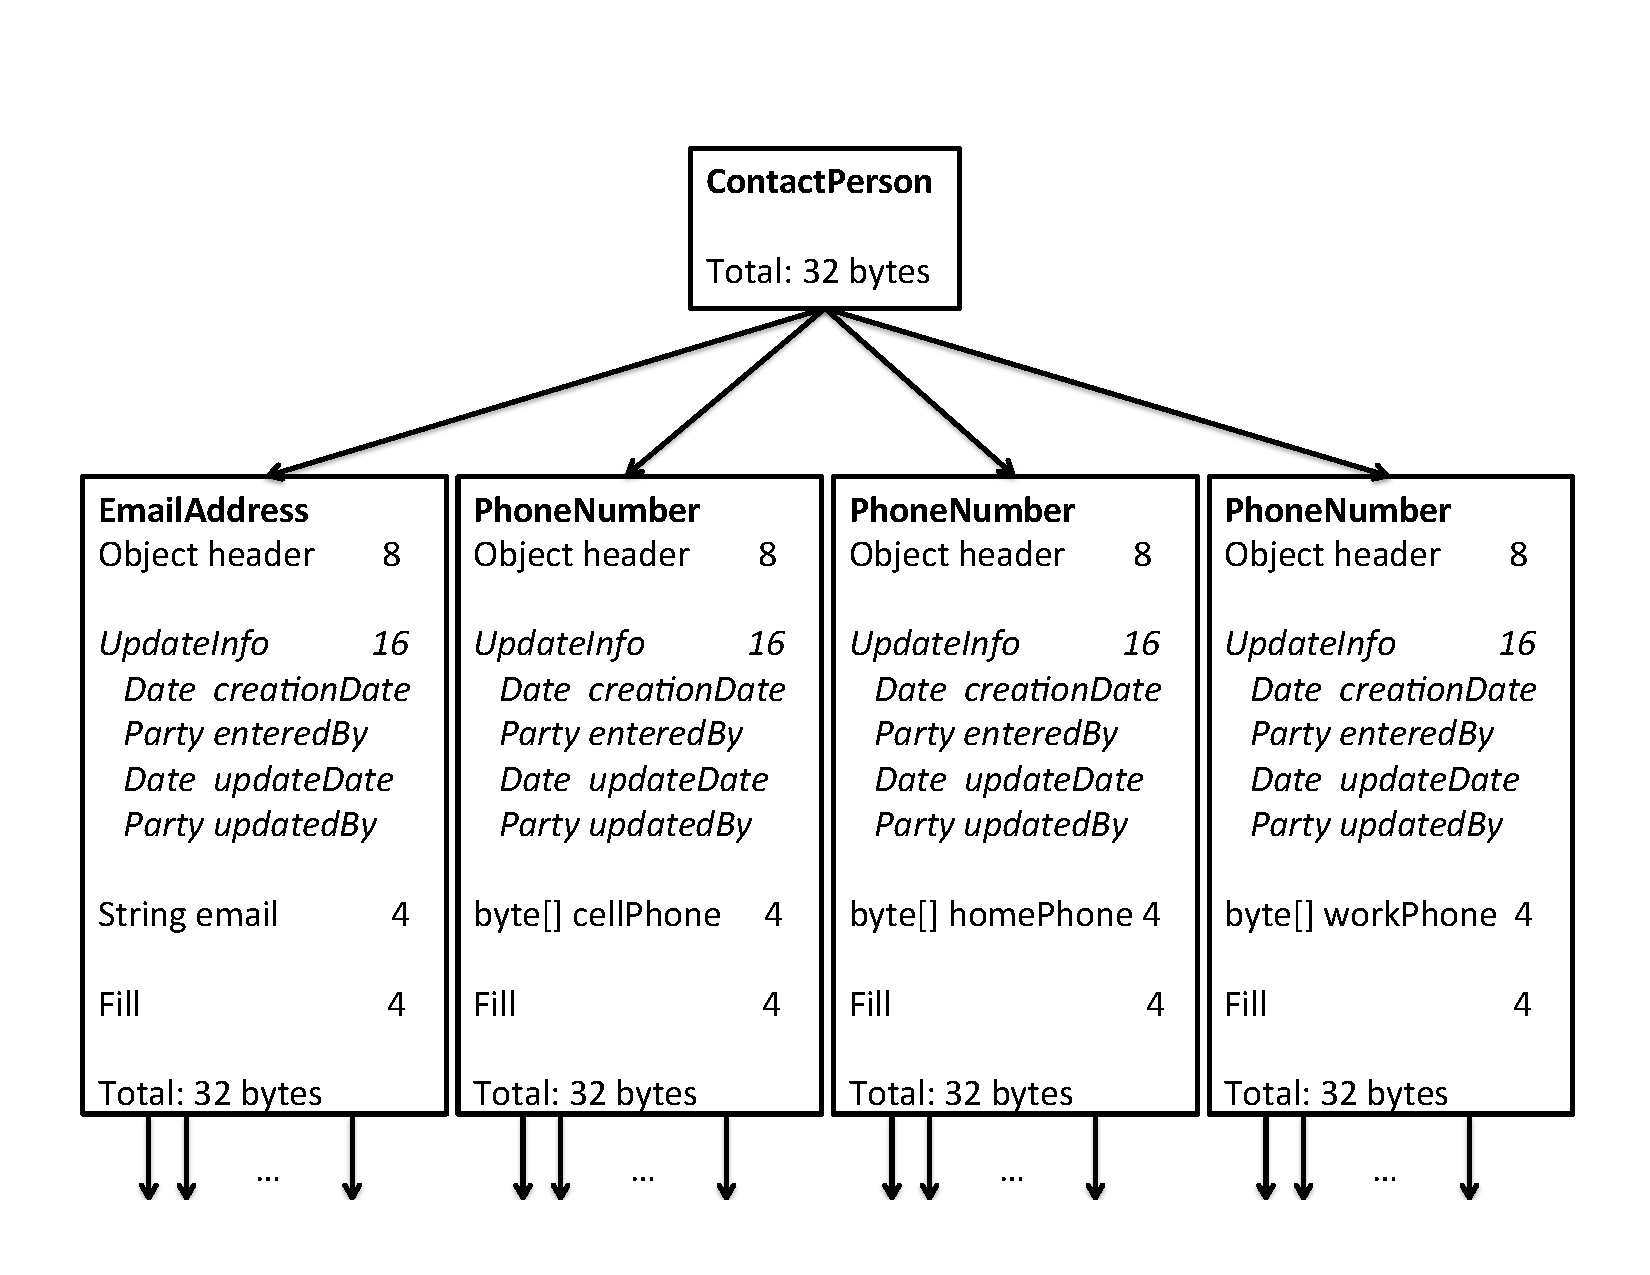
\includegraphics[width=.70\textwidth]{part1/Figures/modelingdatatypes/big-base-class.pdf}
 % \includegraphics{eight-char-string}
  \caption{The cost of associating \class{UndateInfo} with every
  \class{ContactMethod}.}
  \label{fig:big-base-class}
\end{figure}
 
The solution in Figure~\ref{fig:big-base-class} provides a very fine
granularity of functionality. An argument can be made in favor of this
solution, since you lose functionality and flexibility if you only track
updates to \class{ContactPerson}. However, if the program hits a scalabity
problem, it may not be possible to be this casual with memory. Also, an alternate
design may be available that gives the desired functionality in a more memory-efficient way. In this
example, you could implement an update log instead of tracking updates in the objects themselves. Assuming
updates are sparse, this is a much better solution. It is very easy define a subclass without looking closely
at the memory size of its superclasses, especially if the inheritance chain is
long.



\section{Writing Efficient Framework Code}

The storage optimizations described in this chapter assume that you are
familiar with the entire application you are working on. You need to
understand how objects are created and used, and therefore know enough to determine
whether these optimizations make
sense. However, if you are programming a library or framework, you have no way
of knowing how your code will be used. In fact, your code may be used in a
variety of different contexts with different characteristics. Premature optimization ---
making an assumption about how the code will be used, and optimizing for that
case --- is a common pitfall when programming frameworks.  

For example, suppose the online store is designed as a framework
that can be extended to implement different kinds of stores.
For some stores, most products may have an alternate supplier. For other
stores, most products may not.  There is no way of knowing. If the
\code{Product} class is designed so that the alternate supplier is allocated as
a side object, then sometimes memory will be saved and sometimes wasted. 
One possibility is to define two versions of the \code{Product} class, one that
delegates and one that doesn't. The framework user can then use the version
that is appropriate to the specific context. However, this is generally not
practical. 

Frequently, decisions are made that trade space for time.
There are many instances of this trade-off in the Java standard library. For
example, let�s look at  \code{String}, which has three 
 bookkeeping fields: an offset,
a length, and a hashcode. These 12 bytes of overhead consume 21\% of an eight
character string. 
The offset and length fields implement an optimization for substrings. 
That is, when you create a substring, both
the original string and substring share the same character array, as shown in
Figure~\ref{fig:substring}. The offset and length fields in the substring
\code{String} object specify the shared portion of the character array. 
This scheme optimizes the time to create a substring, since there is no new
character array and no copying. However, every string pays the price of the offset
and length field, whether or not they are used. In practice, most Java applications
have far more strings than substrings\cite{}, so a lot of memory is
wasted. Even when there are many substrings,
if the original strings go away, you have a different footprint problem, namely,
saving character arrays which are too big.
\begin{figure}
  \centering
 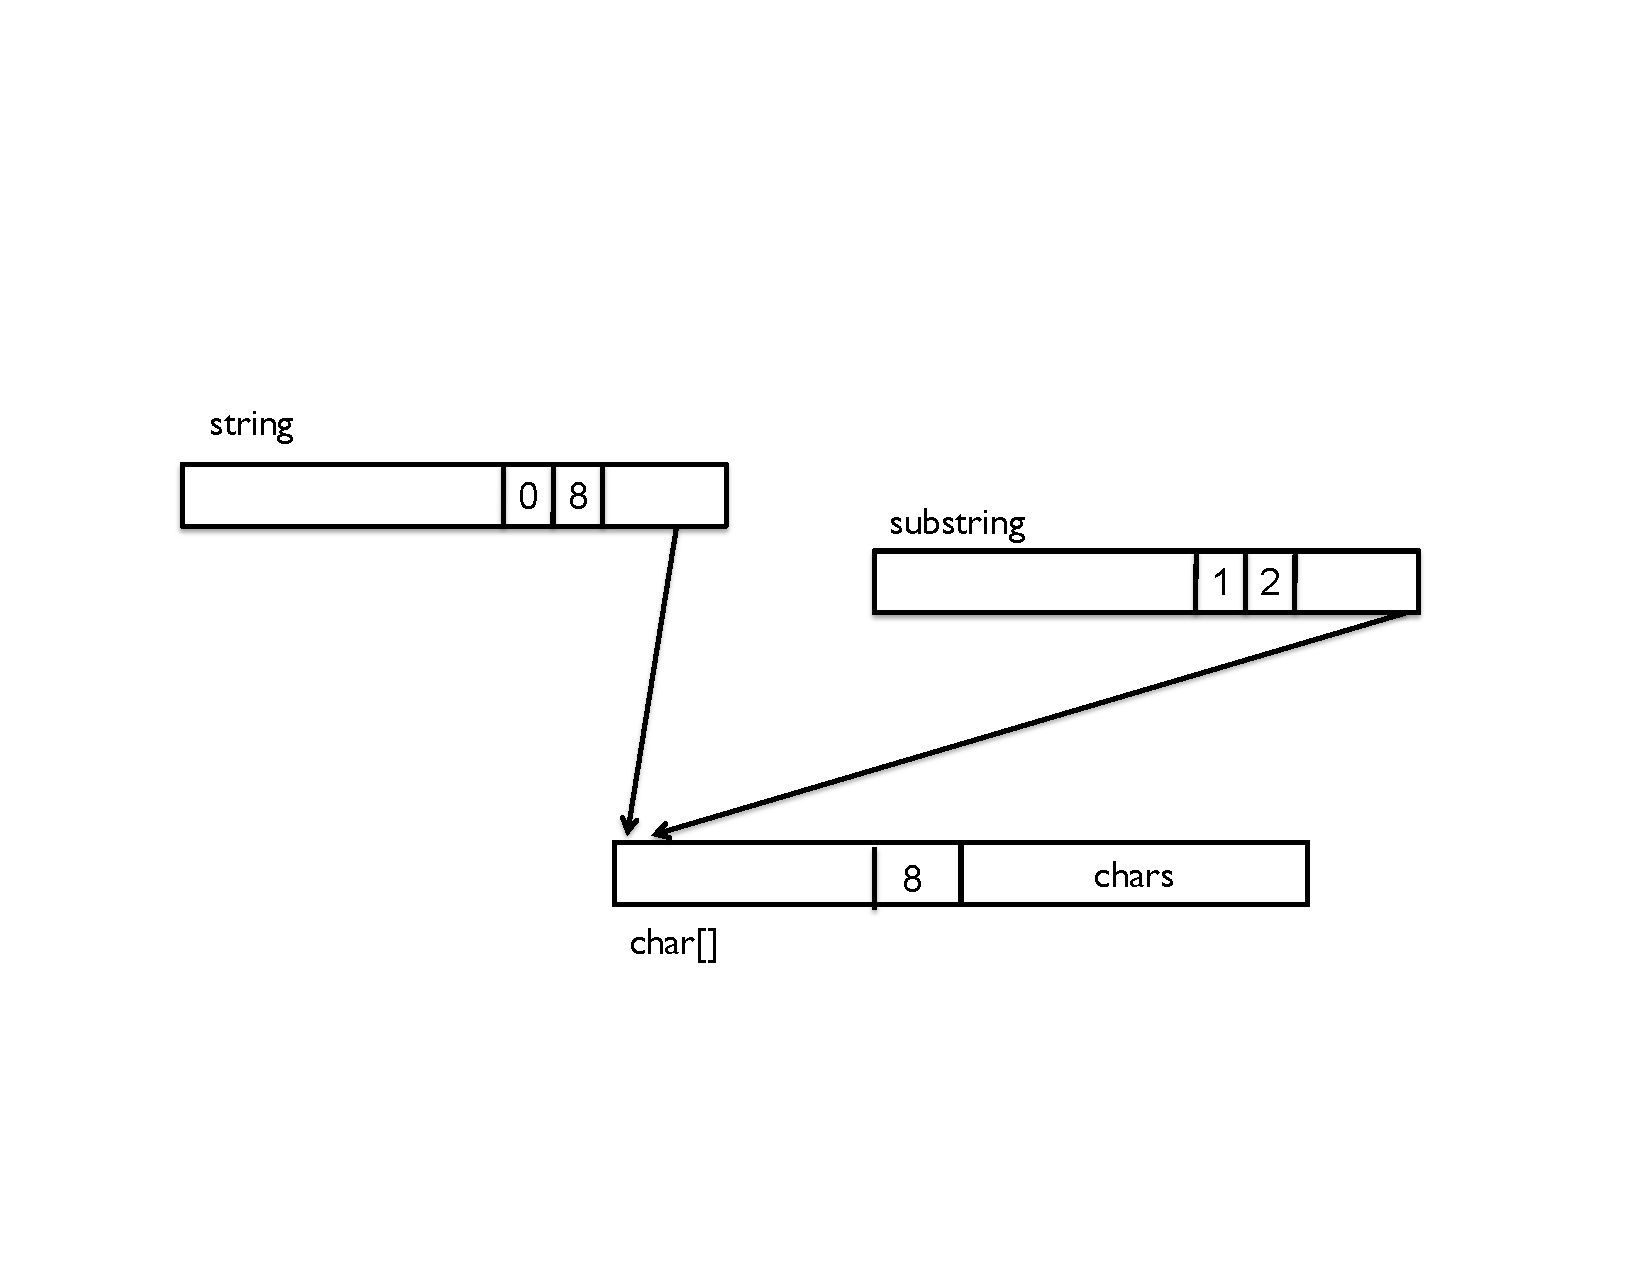
\includegraphics[width=.90\textwidth]{part1/Figures/modelingdatatypes/substring.pdf}
 % \includegraphics{eight-char-string}
  \caption{A string and a substring share the same character array. The length
  and offset fields are needed only in substrings. In all other strings, the
  offset is 0 and the length is redundant.}
  \label{fig:substring}
\end{figure}

%It says that if I ever take a substring of this thing,
% I�m going to be able to share with the origjnal characters of the String This
 %is a theme you will see throughout the JDK, that there�s so many
% optimizations that are done to avoid copies at any cost. Really with a huge
% focus on time, and almost no focus on space whatsoever. So studies we saw at
% TRL, in reality, in the long liv

The third bookkeeping field in \code{String} is a hashcode.
Storing a hashcode seems like a reasonable idea, since it is expensive to
compute it repeatedly. However, you have to be puzzled by the space-time
trade-off, since 
a string only needs its hashcode when it is stored in a \code{HashSet} or a
\code{HashMap}. In both of these cases, the \code{HashSet} or \code{HashMap}
entry already has a field for hashcode for each element. \footnote{There
may be some benefit in saving the hashcode in a \class{String} that's used for
looking up a map entry, but only when the same \class{String} object is used for
lookup repeatedly.}

This is a cautionary tale of premature optimization. Framework
decisions can have a long-lived impact. At the same time, it is difficult to
test new frameworks in realistic settings, or to even predict how they will be used.
For these \class{String} optimizations, it's not clear that there is any performance gain
in real-world applications, as opposed to benchmarks. Meanwhile all
applications must pay the price in memory footprint.

\section{Summary}

Even though Java does not let you control the layout of objects, it is still
possible to make objects smaller by recognizing certain usage patterns.
Optimization opportunities include:

\begin{itemize}
  \item Rarely used fields can be delegated to a side object, or stored in a
  completely separate attribute table.
  \item Mutually exclusive fields can share the same field, provided they have
  the same type.
  \item Fields that have the same value in all instances of a class can be
  declared static.
  \item Redundant fields whose value depends on the value of other fields can
  be eliminated, and recomputed each time they are used.
  \item Inner classes which can be made static will avoid storing a
  hidden \code{this} pointer. 
\end{itemize}

Every field eliminated saves around 4 bytes per object, which may seem small.
However, often several optimizations can be applied to a class, and if the
class has a lot of instances, then these small
optimizations turn out to be significant. They are especially useful in
base classes, where their effect can be multiplied.

Many of these optimizations do not come for free. They trade one kind of cost
for another, and can easily make things worse, depending on the context.
So it's important to look at how your data will be used, and to estimate
and then measure the effect of any optimizations. It's also a good idea to
design your APIs so that classes can be easily refactored
later on:

\begin{itemize}
  \item Callers use interfaces rather than concrete classes.
  \item Callers use factory methods rather than constructors.
\end{itemize}


\chapter{Representing Field Values}
\label{chapter:representing-values}

So far, we have been concerned with the wasteful overhead that can result when
modeling your entities as classes and fields. But what about the field data
itself? Java gives you a number of different ways to represent common datatypes, such
as strings, numbers, dates, and bit flags. Depending on which
representation you choose, the overhead costs can vary quite a bit. 
These costs, hidden in the implementation, are not obvious, and can be
surprisingly high.
In this chapter, we look at the costs of different representations for the most 
commmon datatypes.

\section{Character Strings}
\code{String}s are the most common non-trivial data type found in Java
programs. They are the single largest consumer of memory in most applications,
typically taking up 40-50\% of the heap. We discuss when to use a Java \class{String} to
represent data, and when not to.

%\subsection{External vs. Internal Datatype Forms}
\subsection{Scalars vs. Character Strings}
Character strings are the universal data type, in that all data can be
represented in string form.  For example, I am now typing the integer 347 as a
string of characters in this paragraph, and it is stored in a file as a sequence
of characters. Similarly decimal numbers, dates, and boolean values can be
represented as character strings.
 
In Java programs, it's very common to see scalar data represented as instances
of the Java \class{String} class. This representation makes some sense if the
data is read in and/or written out as characters, since it avoids the
cost of conversion. However, there are several good reasons why it's better
to represent data as scalars whenever possible. First, if you need to perform
any kind of operations on the data, you will need to convert it to use
available datatype operators. If these conversions are performed
repeatedly, then there may be lots of temporaries generated needlessly.  Second,
representing data with specific data types leads to better type checking to avoid bugs. 
Third, specific data types provide a simple form of documentation.
Last but not least, the memory overhead of a string representation is much
higher than the overhead of scalars and even of boxed forms.

\begin{table}
  \centering
\begin{tabular}{llr} \toprule \toprule
& Example & Size \\ \midrule \midrule
integer & int anint = 47; & 4 \\
\midrule
& Integer anint = new Integer(47); & 20 (4+16)  \\
\midrule
& String anint = new String(``47''); & 44 (4+40) \\
\midrule
\midrule
boolean & boolean abool = true; & 1\\
\midrule
& Boolean abool = new Boolean(true): & 20 (4+16) \\
\midrule
& String abool = new String(``T''); & 44 (4+40) \\
\midrule \midrule
enumerated type & enum Gender \{MASCULINE, FEMININE, NEUTER\}; &\\
& Gender agender = MASCULINE; & 4 \\
\midrule
& String agender = new String(``masculine''); & 60 (4+56) \\
\bottomrule \bottomrule
\end{tabular}
\caption{The cost of different ways to represent an integer, a boolean, and an
enumerated type. The size column shows both the field size and the cost of
additional delegated objects.}
\label{tab:data-sizes}
\end{table}

Table~\ref{tab:data-sizes} shows three examples of the cost of different
representations of the same value. In the first example, an integer 47 can be
represented as a 4-byte scalar field, a boxed scalar, or a Java \class{String}. 
The \class{String} is by far the costliest representation, requiring 11 times
the memory of the scalar representation. It has a bloat factor of 95\%.
The effect is similar in the other two examples, a boolean and an enumerated
type. The blowup in memory cost for the \class{String} representation is a
factor of 44 and 15, respectively. In Java, \class{String}s are a very expensive way to
represent scalar values, much more so than in many other languages.

\subsection{StringBuffer vs. String}
Java provides a few different datatypes for character strings, each one
addressing a common use case. \code{String}s are immutable, meant for
string data that never changes once initialized. \code{StringBuffer}s and
\code{StringBuilder}s, on the other hand, are for string data that continues to
be updated over time.

Using long-lived \class{StringBuffer}s to store stable character strings 
can waste memory\footnote{This discussion
applies equally to \class{StringBuffer} and \class{StringBuilder}.}. That's
because \class{StringBuffer}s were designed for building string data over time. They
allocate excess capacity to reduce the time needed for reallocating the
character array and copying the data.  \class{StringBuffer}s will usually
have significant empty space, since they double in size whenever they need to be reallocated. 
Typically, after a string is built up in the \class{StringBuffer}, it is stable, at which point
it should be converted to a \class{String}, so that the \class{StringBuffer} can be
garbage collected. Using a \class{StringBuffer} to facilitate
building a \class{String} is fine, but it should only be used as a temporary
in this case.

\section{Representing Bit Flags}
\label{sec:bit-flags}

A value that can be represented by a single bit seems pretty innocuous from a
memory point of view. However, there are different ways to represent bit flags
in Java, and so it's worth devoting a section to the cost implications of
bit flags. As an example, let's consider a business, open seven days a
week, where employees are assigned to work on different fixed days.  We compare three
different ways of representing work days as bit flags in an employee record.
 
First, you can represent bit flags as boolean fields in an object. For example
employee working days can be directly stored in an employee record:
\begin{shortlisting}

    public class Employee {
    	boolean monday, tuesday, wednesday, thursday, friday, saturday, sunday;
    	
    	public void setWorkMonday(boolean flag) {
    		monday = flag;
    	}
    	..
    }
    
\end{shortlisting}
Each boolean field takes one byte, so each employee contains at least seven
bytes to store workday information. 

Alternatively, you can represent bit flags very compactly as actual bits, and
manipulate the bits via accessor methods. There is more code involved,
but it is isolated in these few methods. Seven days of the week can be stored as
bits in a single byte field:

\begin{shortlisting}
	class Employee {
	
		public final static byte Monday = 0x01;
		public final static byte Tuesday = 0x02;
		public final static byte Wednesday = 0x04;
		public final static byte Thursday = 0x08;
		public final static byte Friday = 0x10;
		public final static byte Saturday = 0x20;
		public final static byte Sunday = 0x40;
		
		private byte workdays;
		
		public void setWorkMonday(boolean flag) {
			if (flag) {
				workdays = (byte)(workdays | Monday);
			} else {
				workdays = (byte)(workdays & ~Monday);
			}
		}
		..
   }
		       
\end{shortlisting}

While compact, these representations are awkward from a coding and
stylistic point of view. A better practice is to represent bit flag values
using an enumerated type, and to represent bit flag fields using Java
\class{EnumSet}s:
\begin{shortlisting}

    class Employee {
 
		public enum Day {MONDAY, TUESDAY, WEDNESDAY, THURSDAY, FRIDAY, SATURDAY, SUNDAY};
    	
    	private EnumSet<Day> workdays = EnumSet.noneOf(Day.class);
    
   	 	public void setWorkday(Day day) {
			if (flag) {
				workdays.add(day);
			} else {
				workdays.remove(day);
			}
		}
	}
    
    
\end{shortlisting}

Since an \class{EnumSet} is an object, this representation is going to
cost more because of delegation. On the Sun JVM, the storage is pretty
well optimized. If the underlying Enum type has less than 64 elements, then an
\class{EnumSet} is represented by one object of size 24 bytes. If the
\code{enum} type has more than 64 elements, then an \class{EnumSet} is two objects, a wrapper plus a
\class{long[]} array. The total cost is 40 bytes plus enough 8-byte
\class{long}s in the array to hold the bit flags. In our example, the cost of storing workdays is 28 bytes per employee:
4 bytes for the reference field and 24 bytes for the \class{EnumSet}. This is considerably
more expensive than storing the bit flags as either bits or booleans. 

When possible, sharing can optimize the cost of 
 \class{EnumSet}s considerably. Suppose
that there are 1000 employees. The cost of storing the workdays for these
employees using an \class{EnumSet} is 28,000 bytes. 
Now suppose 900 employees work Monday
through Friday. These employees can share an \class{EnumSet} representing
these normal working days, reducing the cost to 6,424 bytes.  See \autoref{chapter:sharing-immutable-data}
for more on sharing data.


\section{Dates}

Dates are very common in applications, but representing a date as a data type
can be complex. The complexity comes from the need to represent
universal time  and support conversions, arithmetic operations, and external
representations. In Java, there are different ways of representing times and
dates, and as usual, the more functionality you want, the more memory the
representation takes up.

The simplest and most compact way is to represent a time and date is as a
\code{long} integer:
\begin{shortlisting}
    long timeNow = System.currentTimeMillis();
\end{shortlisting}
The method call \code{System.currentTimeMillis()} returns the current 
date and time in milliseconds since January 1, 1970.  This representation is
perfect for timestamping, performance timings, and relative time
comparisons, however, it is clearly limited.  

For more functionality, you can use the \class{java.util.Date} class:
\begin{shortlisting}
    Date date = new Date();
\end{shortlisting}
This creates a relatively small object (24 bytes) that stores the current date
and time in milliseconds since January 1, 1970. The class \class{Date} itself
supports little other functionality, since most of its original methods have
been deprecated. You can print a \class{Date} object using the default
\code{toString} function. Interestingly, printing a \class{Date} has the funny
side effect of creating another object inside the \class{Date} object, which
doesn't go away!

So how do you get around this lack of functionality?
Because of the semantic richness of dates, Java provides other classes that
support various calendar functions, that operate on \class{Date} objects. For
example, \class{SimpleDateFormat} will print a \class{Date} according to a
specified format:
\begin{shortlisting}
    SimpleDateFormat dateFormat =  new SimpleDateFormat("dd/MM/yy"); 
    System.out.println(dateFormat.format(new Date())); 
\end{shortlisting}

For other date-related functions, you can use 
\class{GregorianCalendar}, which implements the very rich \class{Calendar}
interface and serves as a wrapper for \class{Date}:
\begin{shortlisting}

	GregorianCalendar calendar = new GregorianCalendar();
    Date now = calendar.getTime();
    int year       = calendar.get(Calendar.YEAR);
	int month      = calendar.get(Calendar.MONTH); 
	calendar.add(Calendar.MONTH, 3); 
	..
    
\end{shortlisting}

Now we have functionality, but at what cost? It turns out that a
\class{GregorianCalendar}, created with the default constructor requires six
objects, totalling 424 bytes. This doesn't include the many temporaries
thrown off during the initialization process. This means that if you need to
create many dates in your application, you should not store them as
\class{GregorianCalendars}. Instead, you should store your dates as \class{Date}
objects, and use just one or two instances of a \class{GregorianCalendar} for
operating on the dates:

\begin{shortlisting}
     static calendar = new GregorianCalendar();
     ..
	 Date now = calendar.getTime();
	 calendar.setTime(now);   // a single instance of a 
\end{shortlisting}

\section{BigInteger and BigDecimal}

It is rare that an integer is too big to be represented as an \class{int} or
\class{long}. However, there are rare occasions when a  \class{BigInteger} is
needed. For example, for example, the largest prime
just discovered is over 17 million digits long.
A \class{BigInteger} provides 
arbitrary-precison integer arithmetic functions, which exactly mimics the
functions of the standard integer. 
A \class{BigInteger} is immutable and almost always requires two objects (a
\class{BigInteger} plus an \class{int[]}), for a minimum of 48 bytes total.  The
cost can be more, depending on the number of digits.  The formula for the total size is 
44 + 4*(number of ints needed to represent the integer). 
Because of the cost, unless you need the extra digits, you should just use an integer or long.

Like \class{BigInteger}, the Java class \class{BigDecimal} performs
arbitrary-precision floating point arithmetic. Primarily,
\class{BigDecimal}s are important for accounting and financial applications that
involve currency, where precision and rounding accuracy are critical. With \class{BigDecimal}s,
you can set both the scale, which is the number of digits to the right of the
decimal point, and the rounding method. How to do this is beyond our scope and
covered elsewhere\footnote{do we really need it??}, since our focus is on the
memory cost of the representation.

\class{BigDecimal} has two forms: a compact form and an
inflated form. Most of the time, \class{BigDecimal} uses the compact form,
which is a single 32-byte object that can store a number whose significand's
absolute value is less than or equal to \code{Long.MAX\_VALUE}.
All 18-digit decimal numbers will fit in that, and some 19-digit.  Bigger than
that, the inflated form is required. In the inflated form, \class{BigDecimal}
delegates the storage of the significand to a \class{BigInteger}, which almost always means two additional
objects, bringing the total for BigDecimal to 80 bytes at a
minimum.  

Unfortunately, sometimes a \class{BigDecimal} will become inflated,
since certain arithmetic methods will cause a \class{BigDecimal} to switch to its inflated form in order to perform the operation, and once inflated,
there's no switching back.  The cases are too numerous to predict, so if there's
a concern it's best to look at the heap and see what happens based on actual usage in the 
application.

Similarly, calling \code{toString()} on a \class{BigDecimal} causes it to
save its string representation, in case it is needed again.
This is another example of a performance optimization that 
costs space, built into the library.  This operation adds an extra two objects
retained with the \class{BigDecimal}. 

In summary, a \class{BigDecimal} will take one
object under most circumstances, but can take up to five. Since it is hard to
predict, you just have to beware.

\section{Summary} 

There are common data types just beyond simple primitives that can
take up a lot of space.  These include character strings, bit sets, dates, and
arbitrary-precision numeric data. This chapter shows the costs of various
representations and what the trade-offs are. Not surprisingly, the cost varies
according to functionality, and the main lessor is not to use expensive
representations unless you need the functionality.

\begin{itemize}
  \item  Don't use \class{String} to store data that can be natuarlly
  represented in a more compact data form, such as integer or boolean.
  \item Storing strings in \class{StringBuffer}s can waste a lot of space
  if they are sized much bigger than the data they store.
  \item Even simple bit flags can cause bloat. If you generate lots of objects
  with bitflags, you should make sure you choose the most efficient
  representation.
  \item Beware of storing dates as \class{GregorianCalendar}s.  A
  \class{GregorianCalendar} should only be used and reused as a converter
  object, to perform operations on \class{Date}s.
  \item \class{BigInteger} and \class{BigDecimal} provide arbitrary precision
  arithmetic on integers and decimals, and are needed when this functionality is
  needed. Otherwise, using them just consume a lot of space and time.
\end{itemize}










\chapter{Sharing Immutable Data}

So far, we have been concerned with the wasteful overhead that results from
data representation. But what about the data itself? If you examine any Java
heap, you will find that a
large amount of the data is duplicated. At one extreme, 
there are often thousands of copies of the same boxed
integers, especially 0 and 1. At the other extreme, there may be many
 small data
structures that have the same shape and data. 
And, of course, duplicate strings are extremely common.
This chapter describes various
techniques for sharing data to avoid
duplication, including a few low-level mechanisms that Java provides.

\section{String Literals}
\label{sec:literals}

Duplicate strings are not only one of the
most common sources of memory waste, they are also very expensive, since even
small strings incur a large overhead. Fortunately, it is not
hard to eliminate string duplication. 

 One technique is to represent strings as  
literals whenever possible. Duplication problems arise because dynamically
 created \class{String}s
are stored in the heap without checking whether they already
exist. \class{String} literals, on the other hand, are stored in a
\emph{string constant pool} when classes
are loaded, where they are shared. Therefore, there is a big advantage to
\class{String} literals.

 As an example, suppose an application
reads in property name-value pairs from files into tables:
\begin{shortlisting}
class ConfigurationProperties {
    ..
	void handleNextEntry() {
		String propertyName = getNextString();
		String propertyValue = getNextString();
		propertyMap.put(propertyName, propertyValue);
	}
}
\end{shortlisting}
The \class{String}s stored in \code{propertyMap} are created dynamically. If 
there are just a few distinct property names in all of the input pairs, these
property names will be duplicated many times in the heap.

However, if you know in advance what all of the property names are, then you can
define them once as \class{String} literals, which can be shared among the
entries of \code{propertyMap}.
\begin{shortlisting}
class PropertyNames {
	public static String numberOfUnits = ``NUM_UNITS'';
	public static String minWidgets = ``MIN_WIDGETS'';
	..
}

class ConfigurationWithStaticProperties {
    void handleNextEntry() {
       String propertyName = getNextPropertyName(); 
       String propertyValue = getNextString();
       propertyMap.put(propertyName, propertyValue);
    }
}
\end{shortlisting}
The \code{getNextPropertyName} method reads in a property name, and returns
a pointer to a property name literal, stored in the JVM string
constant pool. Alternatively, defining an enumeration
type to encode property names may be a better stylistic choice.

A common
 mistake is to create a new \class{String}  from a \class{String} literal,
 which is usually completely unnecessary:
\begin{shortlisting}
class PropertyNames {
	public static String numberOfUnits = 
	                           new String(``NUM_UNITS'');
	public static String minWidgets = 
	                           new String(``MIN_WIDGETS'');
	..
}
\end{shortlisting}
Even though the standard library is smart enough to share
character arrays in this case, this code still creates redundant \class{String}
objects in the heap.

Using \class{String} literals to avoid dulication is only possible when the
\class{String} values are known in advance. 
Section~\ref{sec:sharing-pools} introduces the notion of a sharing pool for
sharing dynamic data. Section~\ref{sec:sharing-strings} describes the Java
string interning mechanism, which uses a built-in string sharing pool to
eliminate duplication.

\section{Sharing Pools}
\label{sec:sharing-pools}

Suppose an application generates a lot of duplicated data and the values
are unknown before execution. 
You can eliminate data duplication by using a \emph{sharing pool}, as shown
in Figure~\ref{fig:sharing-pool}. In Figure~\ref{fig:sharing-pool}(a), objects
A and B point to identical data structures.
Figure~\ref{fig:sharing-pool}(b) shows objects A and B sharing the same data
structure, which is stored in a sharing pool.
 \begin{figure}
  \centering
 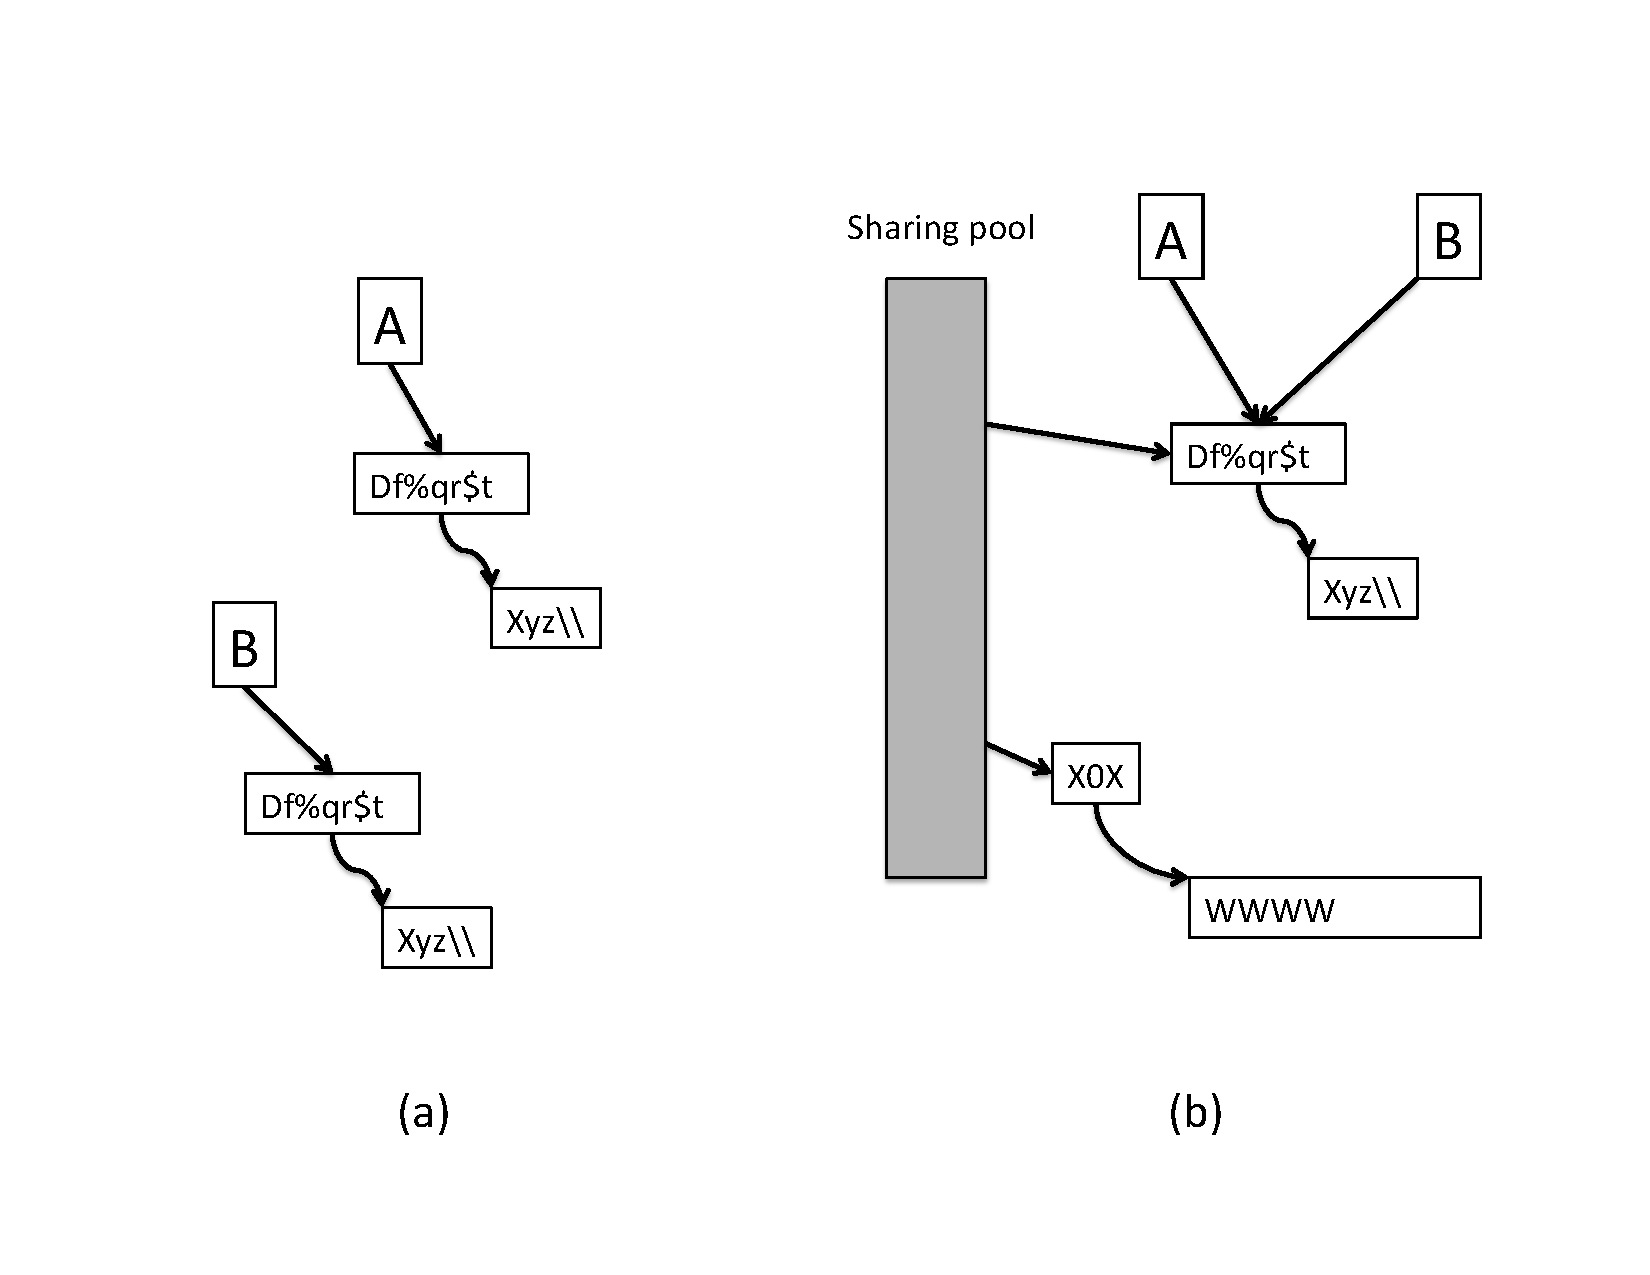
\includegraphics[width=.80\textwidth]{part1/Figures/modelingdatatypes/sharing-pool.pdf}
  \caption{(a) Objects A and B point to duplicate data. (b) Objects A and B
  share the same data, stored in a sharing pool.}
  \label{fig:sharing-pool}
\end{figure}

\callout{callout:sharing-pool}{Sharing Pool}{
A \emph{sharing pool} is a centralized structure that stores 
canonical data values that would otherwise be replicated in many objects.
A sharing pool itself is usually some sort of hash table, although it
could be implemented in other ways.
}

There are several issues that you need to be aware of before using a sharing
pool.
\paragraph{Shared objects must be immutable.} Changing shared data can
have unintended side effects. For example, 
changing A in Figure~\ref{fig:sharing-pool}(b), 
also changes the value of B.

\paragraph{The result of equality testing should be the same, whether or
not objects are shared.}
 In particular, you should never use == on shared objects.
In Figure~\ref{fig:sharing-pool}, \code{A==B} is false in
Figure~\ref{fig:sharing-pool}(a) and true in Figure~\ref{fig:sharing-pool}(b),
 which can lead to very subtle bugs. It is dangerous to use == in any case,
 unless exact object identity is really required.
 
\paragraph{Sharing pools should not be used if there is limited sharing.}
A sharing pool itself adds
memory costs, including additional per-entry costs. If there is not
much sharing, then the memory saved from
eliminating duplicates isn't enough to compensate for the
extra cost, and memory will be wasted instead of saved. 

\paragraph{Shared objects should be garbage collected.}
In Figure~\ref{fig:sharing-pool}(b), the sharing pool stores an object
that no other object is pointing to. Over time, the sharing pool can fill up
with garbage, that is, items that were once needed but not any more. If the
sharing pool is not purged of these unused items, there is a memory
leak that can eventually use up all of memory.

Fortunately, Java provides a few built in mechanisms that take care of some of
these concerns.

\section{String Interning}
\label{sec:sharing-strings}
\index{Interning}

%Before storing a 
%To use a sharing pool, before storing a new
%\class{String}, first check the pool to see if it is already there. If it is,
%reuse it; otherwise, add the new string to the pool. 
%One catch is that if you end up adding many strings to
%the pool that are never reused, then you will waste memory, since the pool
%structure itself has overhead. So you need to have a good idea
%which strings are likely to have duplicate values.

 Since \class{String} duplication is so common, Java provides a built-in string
 pool for sharing \class{String}s, implemented by the native JVM and maintained in
 its internal \emph{perm space}. To share a \class{String}, you simply call the
 method \code{intern} on it, and everything is taken care of automatically.
Since \class{String}s are immutable, sharing is safe. However, the rule about
not using == still holds on shared \class{String}s.
  
In the example from section~\ref{literals},
\class{ConfigurationWithStaticProperties} eliminates property
name duplication but not
property value duplication. Suppose you know that there are
not too many distinct values, but you don't know what they are. In this case,
property values are perfect candidates for interning.
\begin{shortlisting}
 
 class ConfigurationPropertiesWithInterning {
    void handleNextEntry() {
       PropertyName propertyName = getNextPropertyName(); 
       String propertyValue = getNextString().intern();
       propertyMap.put(propertyName, propertyValue);
    }
}
\end{shortlisting}

The call to \code{intern} adds the new property value \class{String}
 to the internal string
pool if it isn't there already, and return a pointer to it. Otherwise, the
new \class{String} is a duplicate, and a previously saved \class{String} is
returned.

Even though interned \class{String} are not stored in the heap, they do incur
native memory overhead, and native memory is not free.
 Interning \class{String}s indiscriminately wastes memory and can result in an
 exception: \code{java.lang.OutOfMemoryError:PermGen Space}. 
There are JVM parameters to adjust the perm space size:
XX:PermSize=128m sets perm size to 128 megabytes, and -XX:MaxPermSize=512m sets
the maximum perm size to 512 megabytes. Fortunately, the JVM performs garbage
collection on the internal string pool, so there is no danger of a memory leak.

TODO: shorten this to a quick forward reference. There is an
important variant of a sharing pool called the Bulk Sharing Pool. Like a normal sharing pool, the goal of a bulk sharing pool is to amortize the
memor costs of storing data. However, rather than mitigate the costs of data
duplication, a bulk sharing pool aims to amortize the costs of Java object
headers across the elements in a pool. This is a topic that stretches notions of
how to store data beyond the normal Java box, and so will be discussed, along
with many similar matters, in \autoref{chapter:large-long-lived}.

 %    * Literal strings within the same class in the same package represent
%     references to the same String object. * Literal strings within different
 %    classes in the same package represent references to the same String
%     object. * Literal strings within different classes in different packages
 %    likewise represent references to the same String object. * Strings
 %    computed by constant expressions are computed at compile time and then
   %  treated as if they were literals. * Strings computed by concatenation at
    % run time are newly created and therefore distinct.
\section{Integer Sharing Pool}

The Java library provides a sharing pool for \class{Integer}s. 
Unlike the string pool, the \class{Integer} pool is initialized at class load
time to store all \class{Integer}s in a fixed range, from -128 to 127 by
default. The method \code{Integer.valueOf(int value)} returns a pointer to an \class{Integer} 
in the pool, provided \code{value} is in range.

Because the \class{Integer} sharing pool is pre-initialized and fixed in size,
it's always a good idea to call \code{Integer.valueOf} instead of the constructor to
create a new \class{Integer}. For example, the following code stores
\class{Integer}s from 1 to 500 in an array:
\begin{shortlisting}
    for (int i = 1; i <= 500; i++) {
        numbers[i] = Integer.valueOf(i);
    }
\end{shortlisting}
For the first 127 numbers, \code{valueOf} returns an existing \class{Integer}. 
For the rest of the numbers, \code{valueOf} returns a new
\class{Integer}.  Calling \class{Integer.valueOf} incurs no extra overhead,
and you never have to worry about wasting memory or getting a
memory exception. The only precaution is avoid using == to compare potentially
shared \class{Integer}s.

There is a JVM parameter to change the size of the \class{Integer} sharing pool:
-XX:AutoBoxCacheMax=100 sets the high value in the pool to 100.

\section{Sharing Objects}

Beyond strings and boxed \class{Integer}s, there are often other kinds of
duplicated objects and data structures consuming large portions of the heap. 
There is no built-in Java mechanism to share objects or data
structures in general, so you have to implement a sharing pool for them from
scratch. All of the sharing pool issues from Section~\ref{sec:sharing-pools} need to be
addressed. The shared objects or structures must be immutable, they must not be
compared using ==, there must be sufficient memory savings from sharing to
justify the sharing pool, and the sharing pool must be not cause a memory leak. 
Note that, in general, \code{equals} is
implemented as ==, so sharing data structures typically requires writing a new
\code{equals} method.

To illustrate a user-written sharing pool, consider a graph where the nodes
have annotations, many of which are duplicates. Both the graph and the
annotations are modified dynamically. The two basic requirements are 1) the
ability to find existing annotations quickly to share them, and 2) the ability
to release annotations that are no longer associated with any node, so they can
be garbage collected.  The second requirement prevents a memory leak. 

Interestingly, none of the common collection classes meet these
requirements out-of-the-box. A \class{HashSet} can store
\class{Annotation}s uniquely, but retrieving an existing \class{Annotation} is not easy. 
The first requirement is best implemented as a \class{HashMap} mapping
\class{Annotation}s to themselves:
\begin{shortlisting}
 	HashMap<Annotation><Annotation>   (1)
\end{shortlisting}


\section{Summary} 

Not only are Java heaps bloated from too much overhead, they
are also bloated from duplicated data. If you know that your application
generates many copies of the same data, then you should find a way to share the
data. Java provides several built-in sharing mechanisms:

\begin{itemize}
  \item The JVM maintains a native sharing
  pool for \class{Strings}. Use \class{String} interning to make use of this
  sharing pool.
  \item The standard library maintains a fixed size pool for
   a fixed range of  \class{Integer}s. You should use \code{valueOf} to create
   \class{Integer}s instead of a constructor.
\end{itemize}
Additionally, Java provides a weak referencing mechanism, which can be used to
implement your own sharing pool.

These mechanisms appear to be clumsy addons that were necessary to solve
problems that came up in practice. But they are better than nothing, and
without them, it would be much harder to share data. 
Whether or not you use these mechanisms, you should remember these four rules:
\begin{itemize}
  \item Shared objects must be immutable.
  \item The result of equality testing should be the same, whether or
not objects are shared.  
  \item Sharing pools should not be used if there is limited sharing.
  \item Shared objects should be garbage collected.
\end{itemize}






\chapter{Collections: An Introduction}
\label{chapter:brief-introduction-collections}

Collections are the glue that bind together your data. 
Whether providing random or sequential access, or
enabling look up by value, collections are an essential part of any design.
In Java, collections are easy to use, and, just as easily, to misuse
when it comes to space. Like much else in Java, they don't come with a price tag
showing how much memory they need. In fact, collections
often use much more memory than you might expect. In most Java applications they are the
second largest consumer of memory, after
strings.  Collection overhead typically accounts
for 10-15\% of the Java heap, and it is not uncommon to see much higher numbers
in individual heaps. The way collections are employed can make or break a system's
ability to scale up.

%awareness of costs; thorough analysis of scalability; whether or not will scale
This and the next three chapters are about using
collections in a space-efficient way. We'll look at typical patterns of
collection usage, their costs, and solutions for saving space. We'll see
techniques for analyzing how local implementation decisions play out at a larger scale.
We will also look at the internal design of a few collection classes.



%Each of the following three
%chapters then goes into depth about a specific way that collections can be
%used. 

%Clarifying requirements can lead to specialized solutions
%can suggest space-saving solutions, so that you are not paying for
%functionality you don't need.
%Look inside a few important collection classes
%

\begin{description}
\item[Chapter~\ref{chapter:brief-introduction-collections}.  Collections: An
Introduction]
Collections serve a number of very
different purposes in your application, each with its own best practices as well
as traps. The current chapter
is a short introduction to issues that are common to
any use of collections. It includes a summary of collection resources
that are available in the standard and some open source alternative
frameworks.
\item[Chapter~\ref{chapter:representing-relationships}.
One-to-Many Relationships] An important use of collections is to
implement one-to-many relationships. These enable quick navigation from an
object to related objects via references. This chapter covers the patterns and pitfalls of
implementing these relationships. At runtime, each relationship
becomes a large number of collection instances, with many containing just a few elements.
%In a product catalog, for example, each product object would have one
%collection instance pointing to that product's suppliers, and another pointing
%to the product's parts.
The main issues to watch for
are: keeping the cost of small and empty collections to a minimum, sizing
collections properly, and paying only for features you really need.

\item[Chapter~\ref{chapter:tables-indexes}. Indexes and Other Large Collection
Structures] A collection can serve as the jumping off
point for accessing a large number of objects. For example, your application
might maintain a list of all the objects of one type, or have an index for
looking up objects by unique key. This chapter shows how to analyze the memory
costs of these structures. The main
issue is understanding which costs will be amortized as the structure grows, and
which will continue to increase. The chapter also covers more complex cases,
such as a multikey map, where there is a choice between a single collection and a multilevel design.
% large structures
% compare design alternatives

\item[Chapter~\ref{chapter:dynamic-records}. Attribute Maps and Dynamic
Records] Many applications need to represent data whose shape is not
known at compile time. For example, your application may read property-value
pairs from a configuration file, or retrieve records from a database
using a dynamic query. Since Java does not let you define new classes on the
fly, collections are a natural, though inefficient way to represent
these dynamic records. This chapter looks at the common cases where dynamic records
are needed, and shows how to identify properties of your data that could lead to
more space-efficient solutions.

%\item[Chapter~\ref{chapter:additional-collection-behaviors}. Additional
%Collection Behaviors] Collections sometimes need to support additional features
%beyond data storage and access. For example,
%you may need to protect a table from inadvertent
%updates, or minimize contention on a map when running in a
%multithreaded environment. Java collections provide these capabilities through
%specialized classes, or through wrappers that alter
%the operation of other collections. This chapter covers the costs of
%these collections.  The granularity
%at which you use them can have a big impact on their memory
%cost.

\end{description}

%Across all of these different uses, collections have some common themes.
%The next section is an overview of issues to
%be aware of in any use of collections. It is followed by a
%survey of collections resources available in the
%standard libraries and some open source alternatives.

\section{The Cost of Collections}
%\section{Designing with Collections}
\label{sec:designing-with-collections}

\paragraph{Choosing carefully}Like other
building blocks in Java, the memory costs of the standard collections are high overall. 
The very smallest of the commonly-used collections, an \emph{empty}
\class{ArrayList}, takes up 40 bytes, and that's only when it's been carefully
initialized. By default it takes 80 bytes. That may not sound like a lot by
itself, but when deeply nested in a design, that could easily be multiplied
by hundreds of thousands or millions of instances.  

There is much that is not under your control in the cost
of collections.
Because the collection libraries are written in Java, they suffer
from the same kinds of bloat we've seen in other datatypes. They have
internal layers of delegation, and extra fields for features that your program
may not use. Some
collection classes have a few options that can help, such as
letting you specify excess capacity allocated initially. On the
whole, though, they do not provide many levers for tuning to different situations. They were
designed mostly for speed rather than space. They seem to have been designed
for applications with a few large and growing collections. Yet many systems have large numbers
of small collections that never grow once initialized. Given all of this, it is important
to be aware of what collections cost, so you can make informed choices as early as possible. 

%In addition, the standard APIs can force you into expensive
%decisions in other parts of your design, such as requiring you to box scalars
%that you place in collections. 
%In this and
%the next four chapters we show you how to figure out those costs, and how
%to avoid some common traps. Armed with this
%knowledge you can choose carefully, ensuring that you are not
%overpaying for your system's needs.

%Even with high costs in general, there are some things that you do
%have some choice over, such as which collection classes to use, and how they
%are initialized.

%and how your data is
%structured to use them effectively. (move to scalability section?)


Fortunately, there are some easy choices you can make that
can save a lot of space. The best thing you can do is to choose carefully
among collection classes. Costs vary
greatly, even among collection classes that may work equally well
in the same situation. 
%making it all the more important to become familiar with what
%collections cost. 
For example, a 5-element \class{ArrayList} with room for growth takes 80 bytes. 
An equivalent \class{HashSet} costs 256 bytes,
or more than 3 times as much. Like other kinds of infrastructure, collections
serve a necessary function, and paying for overhead can be worthwhile. That is, as long as you are not
paying for features you don't need. In the above example, a
69\% space savings can be achieved if the application can do without features
such as uniqueness checking that
\class{HashSet} provides. In Section~\ref{sec:better-designs} we saw a similar
example, achieving a large improvement when real-time
maintenance of sort order wasn't needed. In the next chapters we'll see more
examples of how understanding your system's requirements, along with what
collections cost, can help you make large reductions in memory. 
In general we do not recommend implementing your own collections, at least not
until you've exhausted all other possibilities.

\paragraph{Understanding costs} Collections are pure overhead. Collections are
variable in size, dependent upon the elements they contain. A given
collection class will scale differently in different situations, and it's
important to understand \emph{how a particular collection class
will work in your design}. Some collections were only designed
to be used at a certain scale.
%the same collection
%class will scale differently in different situations. 
For example, a certain map class may work
well as an index over a large table, but can be prohibitively expensive when you
have many instances of it nested inside a multilevel index. 

Each collection class has its own cost
profile that determines how it will scale. This is its fixed
and variable costs, as discussed in Section~\ref{sec:scalability}. 
The fixed cost is the minimum space needed with or
without any elements; the variable cost is the additional space needed to
store each element. The way these costs add up
depends on the context ---
whether there are many small collections or a few large ones. 
High fixed costs take on more significance in smaller collections,
especially when there are many instances of them. High variable costs matter
when there are a lot of elements, regardless of whether the elements are spread across
a lot of small collections or concentrated in a few large ones.
We'll analyze the space needs of very small collections (with number of elements
roughly in the single digits) a little differently from those of larger
collections.
Tables~\ref{tab:small-collections-default} through \ref{tab:empty-collection-costs} in
\autoref{chapter:representing-relationships} show the overhead cost of small and empty collections for some commonly-used
collection classes. The following chapter shows
how to compute costs for larger collections.
\autoref{chapter:jre-comparison} gives more comprehensive information for
additional classes and platforms.



%Collections with high fixed
%costs should only be used for large collections, so that the fixed cost will
%be amortized over a large number of elements.  


%Some collection costs will be amortized as
%more data is stored, others will only continue to grow. 
%Certain collections are designed
%to be used at a certain scale --- when there are a few large collections, not a
%lot of smaller ones.  
It is helpful to look at collection costs 
together with the data they are storing. If a data structure uses expensive collections
to store small amounts of data, than it
will have a high bloat factor, and ultimately the application's ability to
support a large amount of data will be limited. The next chapters show
how to analyze collection costs in the context of your design.
% to ensure that your system will scale when it is time for deployment.
This analysis will help you choose the right collection for your design, or
restructure your data into a more efficient design if necessary.


\section{Collections Resources}

%In the next four chapters we will look in detail at how various
%collection classes can best be used in different situations. 

In this book we focus
mostly on the standard collections. We also include information 
about some alternative, open source frameworks that can be helpful in keeping
memory costs down.

% just a selection throughout the book.  Encourage the reader to explore more
% for themselves.

\paragraph{The Standard Collections} There are some
lesser-known resources in the standard Java Collections framework that provide specialized functionality. Some can help you
save memory if you require only those features.  Others provide useful
features, but can have a significant memory cost if not used carefully.
Table~\ref{tab:lesser-known-collections} is a guide to the resources we discuss
in this book.

\begin{table}
\centering
	\begin{tabular}{l p{6cm} p{4cm}}
	\toprule

	   Resource & Description & Discussed in
	\\ \cmidrule(r){1-1} \cmidrule(l){2-2} \cmidrule(l){3-3}
	\class{Collections} statics & Memory-efficient
	implementations of empty and singleton collections. &
	Sections~\ref{sec:empty-collections}, \ref{sec:mostly-small-collections}
	\\ 
	& Unmodifiable and synchronized
	behaviors are added via collection wrappers. Can be costly if used at too fine
	a granularity. & Sections~\ref{sec:unmodifiable-collections},
	\ref{sec:synchronized-collections}
	\\
	\class{Arrays} statics & Provides static methods if you need to create
simple collection functionality from arrays & Section~\ref{sec:better-designs}
shows one example
	\\
	\class{IdentityHashMap} & Lower-cost map when using an object reference as key
	& %Section~\ref{}
	\\
	\class{EnumMap} & Compact map when keys are \class{Enum}s & %Section~\ref{}
	\\
	\class{EnumSet} & Compact representation of a set of flags &
	Section~\ref{sec:bit-flags}
	\\
	\class{WeakHashMap} & Supports one common scenario for managing object lifetime
	using weak references. &
	%Section~\ref{}
	\\
	Java 1 collections & Some classes in the earlier, Java
1 libraries, like Vector and Hashtable, are a lower-cost choice 
in some contexts where synchronized collections are needed &
Section~\ref{sec:synchronized-collections}
	\\
	\class{ConcurrentHashMap} & Hash map when contention is a concern. Avoid use at
	too fine a granularity. & %Section~\ref{}
	\\
	\bottomrule
	\end{tabular}
	\caption{Some useful resources in the Java standard library}
	\label{tab:lesser-known-collections}
\end{table}


\paragraph{Alternative Collections Frameworks} In addition to the standard Java
classes, there are a number of open source collections frameworks available. Some are designed
specifically to improve space and time efficiency, while others are aimed at
making it easier to program, adding commonly needed features not
found in the standard libraries. 
The alternative collections frameworks can be helpful in two ways when it comes to saving memory. First,
some frameworks provide space-optimized collection implementations. Second, some frameworks
provide classes that make it easier to manage object lifetime. Building your
own object lifetime management mechanisms, for example a concurrent cache, can
be error-prone (see, for example, Section~\ref{}). Well-tested implementations
will save you a lot of effort, and can lead to better overall use of space.
Keep in mind that not all alternative collection classes have
been optimized for space.
Some of them actually take up more space than a similar design using the
standard collections. As always, there is no substitute for analyzing space costs empirically.
%analyzing space usage yourself


In this book we'll look at four of the most recent and relevant
open source collections frameworks. In the next few chapters we'll look at how
you can use some of these classes to solve specific problems.
Table~\ref{tab:alternative-collections} gives a summary of the capabilities that
we discuss (sometimes only briefly). This is only a sampling of what's out
there. We encourage you to further explore these and other frameworks on your own.
%on your own

The Guava framework, which grew out of the Google Collections, is
designed primarily for programmer productivity, providing many useful
features missing from the standard Java collections. 
Although space usage has not been the main focus, it does include some
specialized classes, for example the immutable collections, that are more
space-efficient than their general-purpose equivalents. Guava's \class{MapMaker}
class provides very general support for 
building caches and other lifetime management mechansisms, with optional support
for concurrency. While most open source frameworks provide some level of compatibility with the
standard collections APIs, Guava has made compatibility a priority.

The Apache Commons Collections framework has similar objectives to the Guava
framework, focusing mostly on programmer productivity rather than on
efficiency per se. 
%Of the two, Commons has been around longer. However, as of this writing it
% there have not been recent releases, 
It does however provide some capabilities for saving memory, such as
maps and linked lists with customizable storage, and specialized 
maps that contain just a few elements. It also provides lifetime management
support through its \class{ReferenceMap} class, in a less general
manner than the Guava equivalent. As of this writing,
the Commons API has not been updated to take advantage of generics.

The GNU Trove framework has time and space efficiency as its main goal.
From a memory standpoint its highlights are: collections of primitives that
avoid boxing and unboxing;  map
and set implementations that are lighter weight than the standard ones; and
linked lists that can be customized to use less memory.

The fastutil framework has similar goals to Trove, primarily time and space
efficiency. Like Trove, fastutil provides primitive collections, along with
lighter-weight implementations of maps and sets. Some other memory-related
features include array-based implementations for small
maps and sets, and support for very large arrays and collections when working
in a 64-bit address space.

Important note: there are many kinds of open source licenses. Each has different
restrictions on usage. Make sure to check with your organization's open
source software policies to see if you may use a specific framework in 
your product, service or internal system.

\begin{table}
\centering
	\begin{tabular}{p{6cm} p{3cm} p{4cm}}
	\toprule

	   Feature & Supported by & Discussed in
	\\ \cmidrule(r){1-1} \cmidrule(l){2-2} \cmidrule(l){3-3}
	Primitive collections & fastutil, Trove & Section~\ref{}
	\\
	\\
	Lighter-weight maps and sets of objects & fastutil, Trove & Section~\ref{}
	\\
	\\
	Immutable collections & fastutil, Guava & Section~\ref{}
	\\
	\\
	Small collections & Commons (maps only), fastutil & Section~\ref{}
	\\
	\\
	Customized linked list storage & Trove & Section~\ref{}
	\\
	\\
	Maps with weak/soft references & Commons, Guava & Chapters~\ref{} and ~\ref{}
	\\
	\\
	Caches & Guava & Section~\ref{}
	\\
	\bottomrule
	\end{tabular}
	\caption{A sampling of memory-related resources available in open source
	frameworks}
	\label{tab:alternative-collections}
\end{table}

%collection classes buried in other frameworks

\section{Summary}
Using collections carefully can
make the difference between a design that scales well and one that
doesn't. Some items to be aware of when working with collections:
\begin{itemize}
  \item The standard Java collections were designed more for speed than for
  space. They are not optimized for some common cases, such as designs with many small
  collections. In general the Java collections use a lot of memory.
 %not designed for the ways they are actually used.
  \item Collections vary widely in their memory usage. Awareness of
  costs is an essential first step in choosing well. Sometimes there is a less
  expensive choice of collection class available, either from the standard
  library or from open source alternatives. Initialization options can also make
  a difference.
  \item The same collection class will scale differently depending on its
  context. Ensuring scalability means
  analyzing how a collection's fixed and variable costs
  play out in a given situation. Watch out for: collections with
  high fixed costs when you have a lot of small collections, and 
  collections with high variable costs when you have a
  lot of elements.
  \item Analyzing your application's requirements, specifically
  which features of a collection you really need, can suggest
  less expensive choices.
\end{itemize}

\chapter{One-to-many Relationships}
\label{chapter:representing-relationships}

One-to-many relationships
%such as those in an entity-relationship model,
are typically implemented in Java using the standard library collection classes.
Each object maintains a collection of the objects related to
it along a given relationship. Since one-to-many relationships are such an
important part of most data models, it is not uncommon for Java applications to
need hundreds of thousands, or even millions, of collections.
Therefore, simple decisions, like which collection class to choose,
when to create collections, and how to initialize them,
can make a big difference on memory cost.
This chapter shows how to lower memory costs when implementing
relationships with collections.
 
 \section{Choosing the Right Collection for the Task}
 \label{section:choosing-collection}

The standard Java collection classes vary widely in terms of how much memory they use.
Not surprisingly, the more functionality a collection provides, the more
memory it consumes. Collections range from simple, highly efficient
\class{ArrayList}s to very complex
\class{ConcurrentHashMap}s, which offer sophisticated concurrent access
control at an extremely high price. 
Using overly general collections, that provide more functionality than
really needed, is a common pattern leading to excessive memory bloat.
This section looks at what to consider when choosing a collection to
represent a relationship. 

Using collections for relationships often results in many small or
empty collections.  That's because for a given relationship there are
usually lots of objects that are related to either just a few other
objects or to none at all.
When there are lots of collections with only a few entries, you need to ask  whether
the functionality of the collection you choose is worth the memory cost of that
functionality\footnote{We'll use the shorthand
\emph{relationship} to mean a one-to-many relationship, unless otherwise noted. 
We'll also use \emph{small collection} to mean a very small collection, where
the number of elements is roughly in the single digits.}

To make this discussion more concrete, let's return to the product and supplier example 
from section~\ref{sec:rarely-used}, and change it a little
 bit. Instead of only one alternate supplier, a product now may have multiple
 alternate suppliers, and each product stores a reference to a collection of alternate suppliers. An obvious choice is
 to store the alternate suppliers in a \class{HashSet}:
 \begin{shortlisting} 
class Product {
	String sku;
	String name;
	.. 
	HashSet<Supplier> alternateSuppliers;
}

class Supplier {
	String supplierName;
	String supplierAddress;
	String sku;
}
\end{shortlisting}


Suppose there are 100,000 products that each have four alternate suppliers on
average. Figure~\ref{fig:product-hashset} shows an entity-collection diagram for
the relationship between products and alternate suppliers.
 \begin{figure}
  \centering
 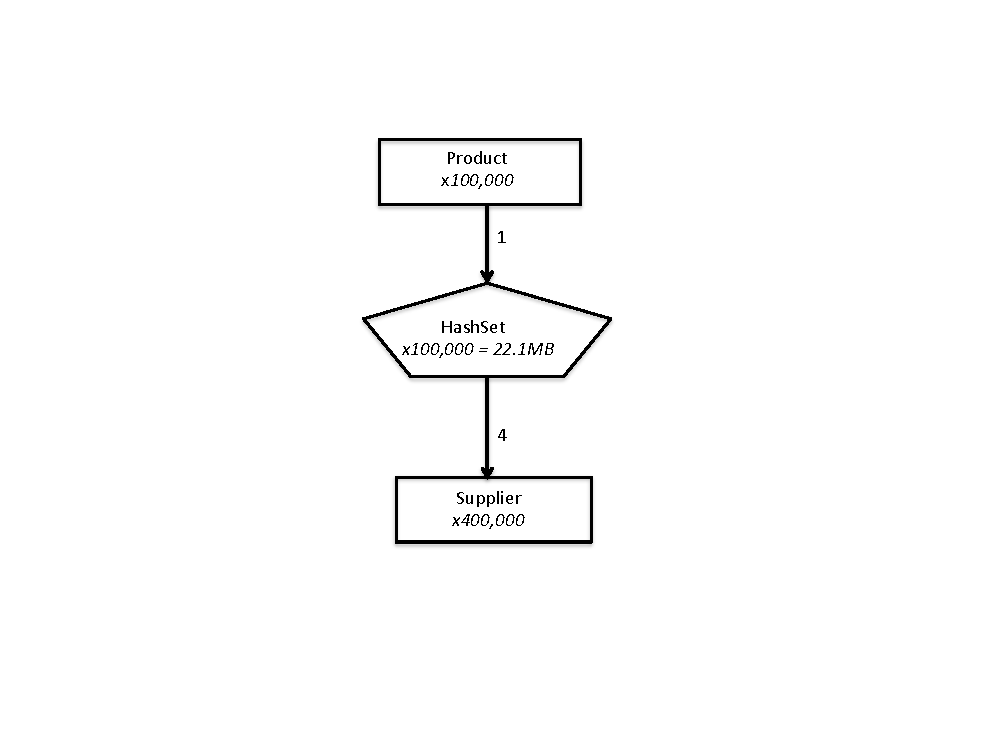
\includegraphics[width=.80\textwidth]{part1/Figures/collections/product-hashset.pdf}
 \caption{A relationship between products and alternate suppliers.
  Stored as one
  \class{HashSet} of alternate \class{Suppliers} per \class{Product}.}
  \label{fig:product-hashset}
\end{figure}


Using a \class{HashSet} for alternate suppliers turns out to be a
very costly decision. The alternate suppliers are represented by 100,000
very small \class{HashSet}s, each consuming 232 bytes, for a total cost of 22.1MB. 
This cost is all overhead.
It's hard to think of a good reason why such a heavy-weight collection should ever be used
 for storing just a few entries, and yet, this pattern is very, very common. For
 small sets, \class{ArrayList} is almost always a better choice. \class{HashSet}
 does maintain uniqueness, but enforcing uniqueness
in the data model is not always needed. Many applications
 perform this check in their loading code. If it is
important to guarantee uniqueness in the data model, it can be enforced for an
\class{ArrayList} with  little extra checking code, and usually without significant performance
 loss when sets are small.  Figure~\ref{fig:product-arraylist} shows improved memory usage with
 \class{ArrayList}. Each \class{ArrayList} incurs 80 bytes of overhead, approximately a third the size of
 a \class{HashSet}.
 \begin{figure}
  \centering
 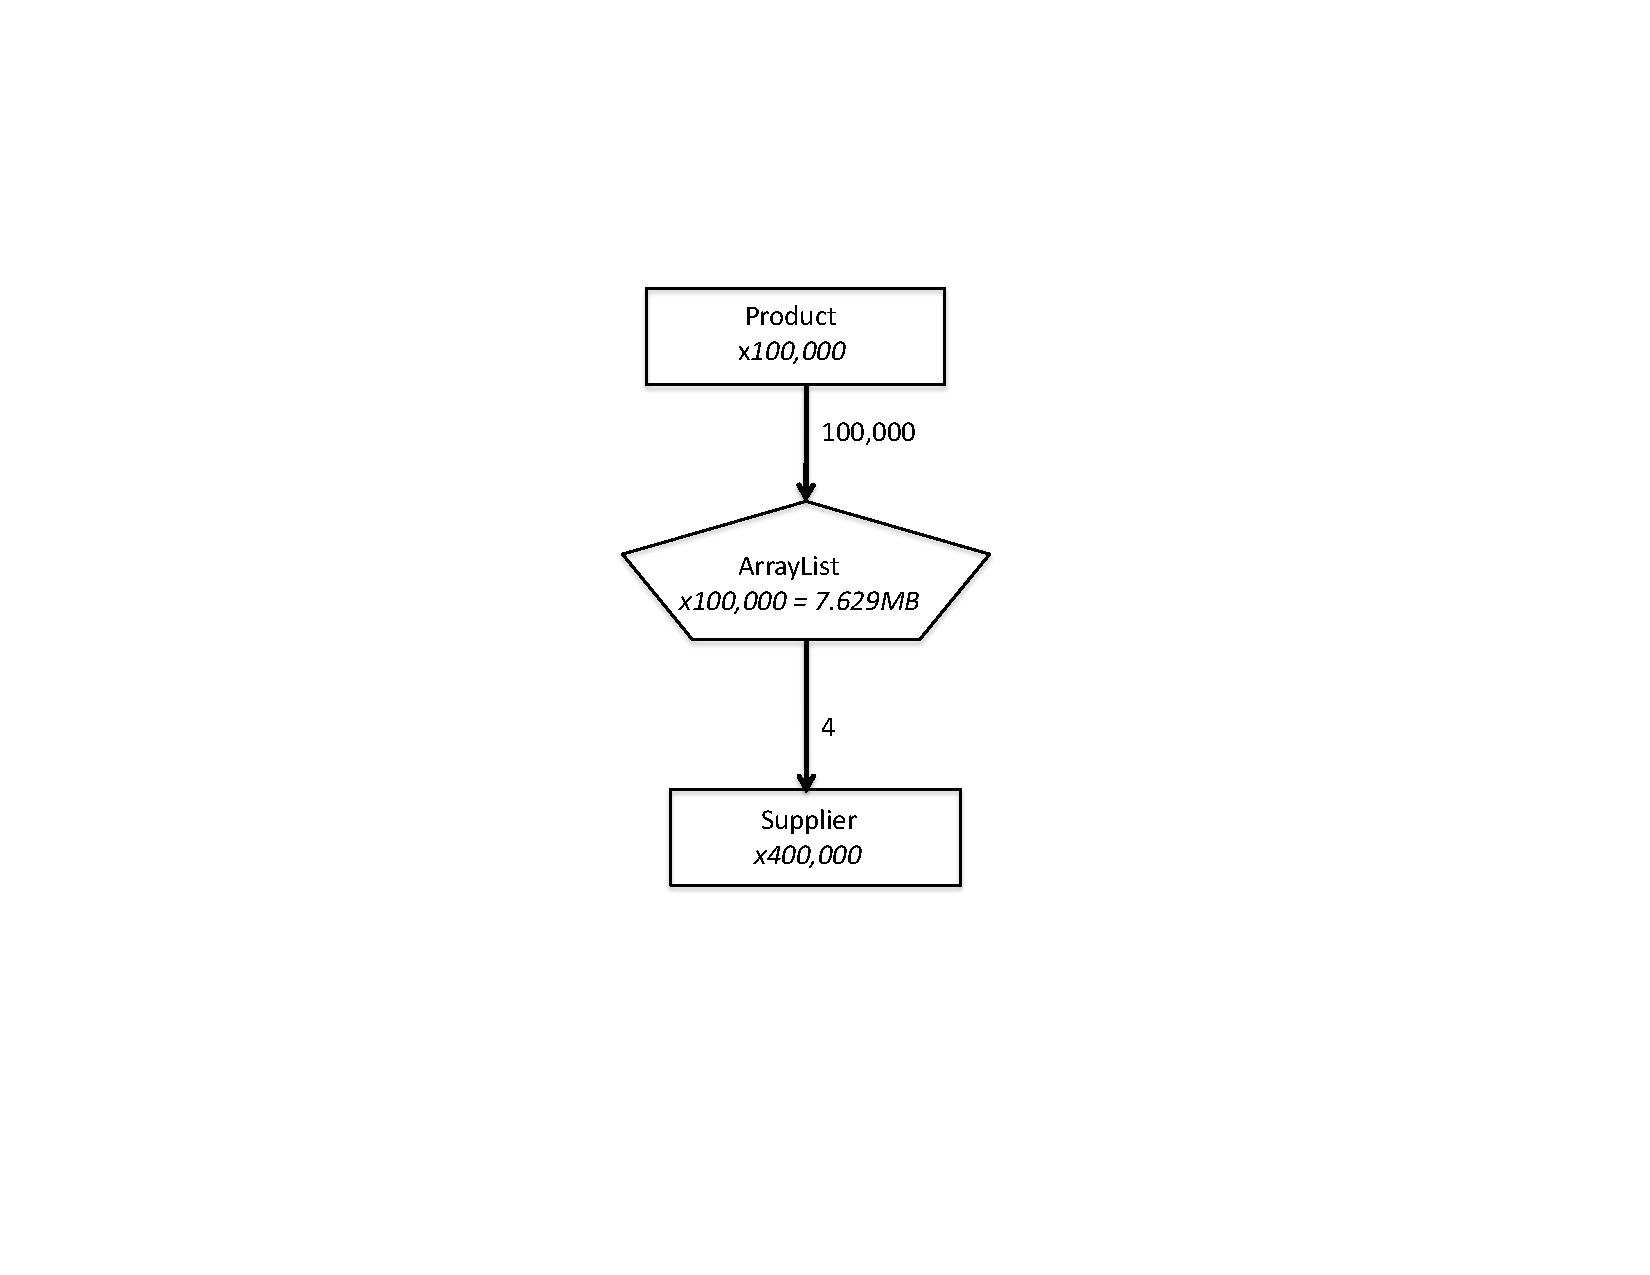
\includegraphics[width=.80\textwidth]{part1/Figures/collections/product-arraylist.pdf}
 \caption{A relationship between 100,000 products and alternate suppliers,
 where the alternate \class{Supplier}s associated with each
 \class{Product} are stored in an \class{ArrayList}.}
  \label{fig:product-arraylist}
\end{figure}
This simple change saves 14.5MB. 


\section{Inside Small Collections}
\label{sec:collectioncost}
Let's look inside a \class{HashSet} to see why it is so much bigger than an
\class{ArrayList}.
The structure of a \class{HashSet} is shown in
Figure~\ref{fig:inside-hashset}. All
collections have a similar basic structure: a wrapper
which remains stable, and an internal structure that changes as entries are
added and removed.

The standard library designers implemented
\class{HashSet} by delegating its work to a degenerate \class{HashMap},
that is, one with keys but no values.
The \class{HashSet} object is therefore just a wrapper, and it points to a
\class{HashMap} wrapper. All collections have
wrapper objects, but a \class{HashSet} has two of them. 
%Together they incur a fixed cost of 56 bytes.

\class{HashMap} itself uses a \emph{chaining}
design. Its internal structure is an array of hash buckets, with initial size of
16 by default.  Each bucket is a linked
list of \class{HashMap\$Entry} objects. Each entry object
points to an element of the user's data, in other words, to a key and value.

 \begin{figure}
  \centering
 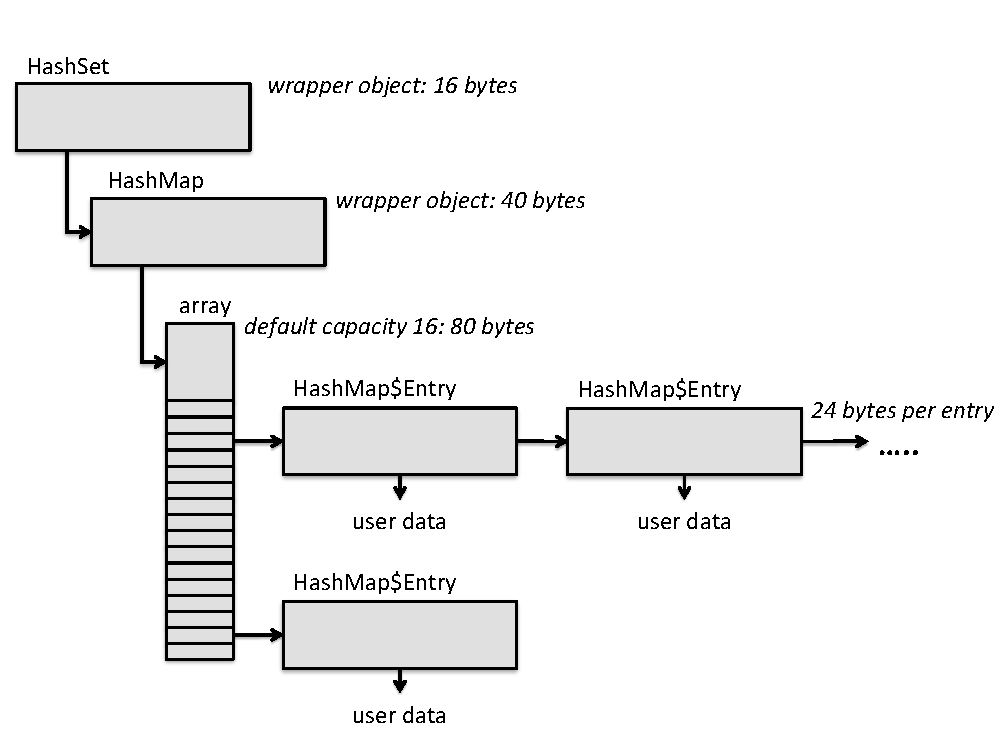
\includegraphics[width=.80\textwidth]{part1/Figures/collections/inside-hashset.pdf}
  \caption{A look inside a \class{HashSet}. Shown with 3
  entries.}
  \label{fig:inside-hashset}
\end{figure}

In contrast, \class{ArrayList} is a simpler structure, as shown in
Figure~\ref{fig:inside-arraylist}. It's an expandable array,
consisting of a wrapper object and an array.  The array points directly to the
user data. The array has an initial size of 10 by default.  As a result of its
simpler design \class{ArrayList} has a smaller fixed cost and a smaller
variable cost than \class{HashSet}.

The fixed cost is the memory needed before any entries are added.
For a \class{HashSet} the fixed cost consists of two wrapper objects, taking 56 bytes, plus
the array's \jre overhead and 16 slots, bringing the total to 136 bytes. We are including the
array's empty slots as a fixed cost since they are allocated right from the start
\footnote{Once a collection grows beyond its initial size, we'll treat
treat excess capacity as a variable cost, as we discuss in the next chapter.
%This is because growth policies allocate excess capacity
%in proportion to the size of the collection
}
\footnote{\class{HashSet} often has another
fixed cost, not shown in our figures.  The first time you iterate over
the set, a 16-byte \class{HashMap\$KeySet} is created and retained for the lifetime of
the set.}.
The fixed cost of an \class{ArrayList} is considerably
lower, a total of 80 bytes. That includes its wrapper object and default
10-element array. Fixed costs matter most in
small collections. As collections grow they become less significant.

A \class{HashSet} maintains a \class{HashMap\$Entry} object for 
each entry, at 24 bytes each. This is its
variable cost, that is, the incremental cost of storing an
entry. It is much higher than that of an \class{ArrayList}, which
use a 4-byte array slot to point to each entry.
A lower variable cost means that \class{ArrayList} scales much
better than \class{HashSet} for large collections. The variable cost also
adds up for small collections, whenever you have a lot of instances of them.  
%Note that we treat the variable cost of a small \class{ArrayList} to be 0,
% since we've already counted the 10 initial slots in the fixed cost.
 \begin{figure}
  \centering
 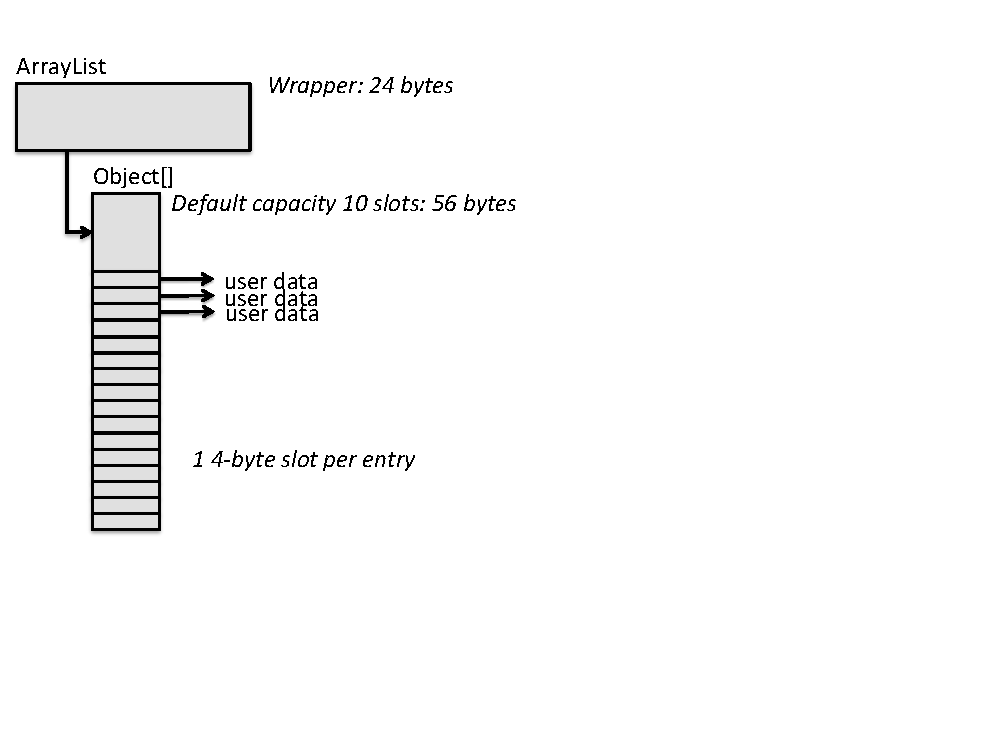
\includegraphics[width=.80\textwidth]{part1/Figures/collections/inside-arraylist.pdf}
 \caption{Inside an \class{ArrayList}. Shown with three
 entries and default capacity. \class{ArrayList} has a relatively low
 fixed overhead, and is scalable.}
  \label{fig:inside-arraylist}
\end{figure}
 

In summary, why does \class{HashSet} take more space than \class{ArrayList}?
We can see a number of reasons. Some of the extra cost is because of
additional functionality, such as providing uniqueness checking and entry
removal, in constant time.
\class{HashSet} is also optimized for performance, and sacrifices memory 
under the assumption that \class{HashSet}s will contain a large number of
elements. The decision
to reuse the more general \class{HashMap} code adds to the memory needed,
especially the fixed cost. Other extra costs
are due to unavoidable Java overhead.
Our guess is that the collection class developers would be surprised by the relationship usage
pattern that results in hundreds of thousands of small \class{HashSets}. 
%Why bother
%implementing expandable structures and clever hashing algorithms for only a few
% entries? 
This mismatch between collection implementation and usage is 
a leading cause of memory bloat. 
%The overhead cost of a \class{HashSet} is
%remarkably high. Creating many small collections multiplies this basic
% infrastructure cost, which is all overhead, filling the heap. 

%The fact that \class{HashSet} delegates to \class{HashMap} inflates its fixed
%cost in two ways: the cost of the extra wrapper object, and the cost of fields
%in the \class{HashMap} that aren't needed when it's used as a set. 
%Note that since the \class{HashMap\$Entry} class is designed for
%a \class{HashMap}, its value field is not used.

 
%Let's look now at some additional choices for small collections.
Table~\ref{tab:small-collections-default} compares the memory costs of four
common classes from the standard libraries.
The table shows bytes needed when each collection contains just a few
entries, plus fixed and variable costs for computing the memory needed for small sizes
in general. All have been allocated with default capacity.
%and the default size when the collection is just allocated without entries, and
% any additional entry cost. 
These costs have been calculated based on the \oracle \jre,
using the techniques described in Chapter~\ref{chapter:delegation}.
%The various other Java standard
%library implementations in circulation have costs
%similar to these. 
You can calculate costs for similar classes using the same methodology.
\autoref{chapter:jre-comparison} has more information about additional classes
and \jre platforms.


\begin{table}
\centering
 		\begin{tabular}{l||r||r||rrl}
 		\toprule
	 	 Collection & with 1 entry & with 4 entries & \multicolumn{3}{c}{with n entries}\\
	 	 & & & fixed & variable & comments \\
	 	 \midrule
	 	ArrayList & 80 & 80 & 80 & 0 & for n in 0..10 \\
 		HashMap & 144 & 216 & 120 & 24 & for n in 0..12 \\
 		HashSet & 160 & 232 & 136 & 24 & for n in 0..12 \\
 		LinkedList & 72 & 144 & 48 & 24 & for any n \\
	 	\bottomrule
	 	\end{tabular}
	 	
	\caption{Cost of some common collections when they
	contain very few entries and are allocated with default capacity. Variable
	cost is the cost per entry, above the fixed cost of the collection. Costs apply only within the specified
	range.}
	\label{tab:small-collections-default}
\end{table}

\begin{figure}
  \centering
 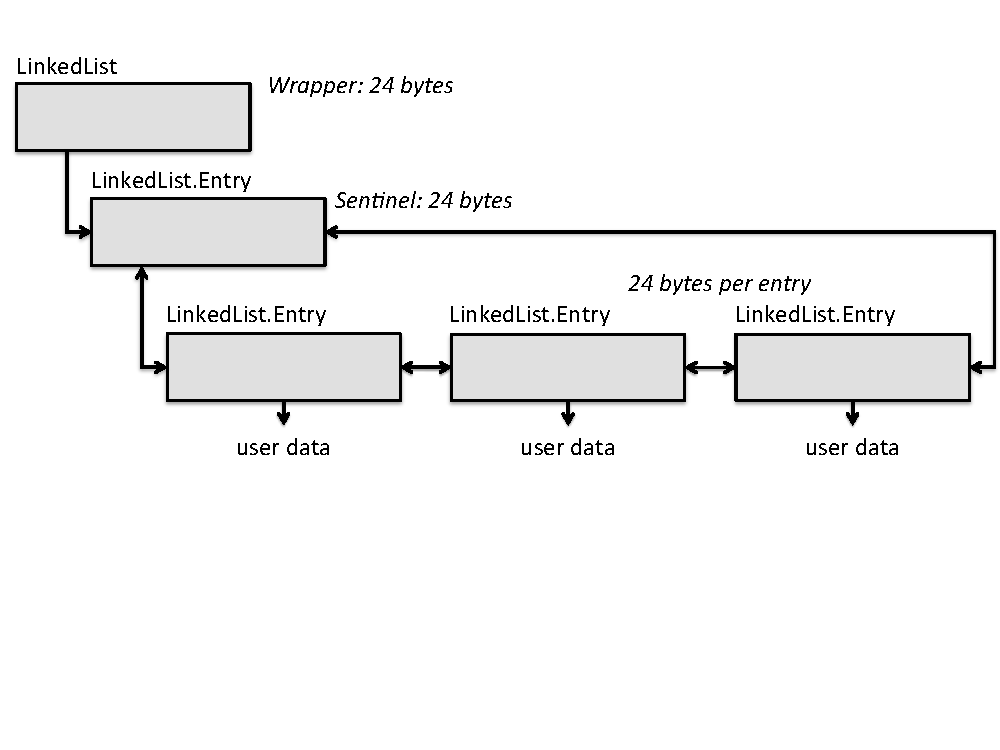
\includegraphics[width=.80\textwidth]{part1/Figures/collections/inside-linkedlist.pdf}
 \caption{A look inside a \class{LinkedList}. Shown with 3
  entries.}
  \label{fig:inside-linkedlist}
\end{figure}

Let's now look at one more choice, \class{LinkedList}, useful when ordering is
needed and there are frequent insertions or deletions.
\autoref{fig:inside-linkedlist} shows its internal structure. A
\class{LinkedList} always has one wrapper object, plus a dummy entry object that
acts as an end-of-list sentinel, presumably for performance reasons. The total
fixed cost is 48 bytes.
\class{LinkedList}, just like \class{HashSet}, \class{HashMap}, and
\class{TreeMap}, is an \emph{entry-based} collection, where an internal entry object
is allocated for each element in the collection. Each \class{LinkedList.Entry}
requires 24 bytes, the variable cost of the collection. Entry-based collections
have higher variable costs than \emph{array-based} collections,
such as \class{ArrayList}, which point directly to the user data from array
slots.
The combination of fixed and variable costs can make \class{LinkedList} an
expensive choice even at small sizes.  From
\autoref{tab:small-collections-default} we can see that a 4-element
\class{LinkedList} is much larger than the equivalent \class{ArrayList}. Again, for such
small collections it's worth
asking what the performance gains
are in practice, compared to an array-based representation.  In the next chapter
we'll look at a few examples of array-based maps and sets from some open source
frameworks, in the context of larger collections. A few of these are appropriate
for small collections as well.




\begin{table}
\centering
 		\begin{tabular}{l||rr||rr}
 		\toprule
	 	 Collection & \multicolumn{2}{c}{with 1 entry} & \multicolumn{2}{c}{with 4 entries}\\
	 	 & default & minimum & default & minimum \\
	 	 \midrule
	 	ArrayList & 80 & 40 & 80 & 56 \\
 		HashMap & 144 & 80 & 216 & 184 \\
  		HashSet & 160 & 96 & 232 & 200 \\
 	 	\bottomrule
 	 	\end{tabular}
	\caption{The effect of capacity on the cost of some small collections,
	comparing the default capacity with the minimum to accomodate the number of entries.
	For \class{HashMap} and \class{HashSet}, 1 entry requires a capacity of 2, and 4 entries requires a capacity
	of 8.}
	\label{tab:small-collections-minimum-samples}
\end{table}

\begin{table}
\centering
 		\begin{tabular}{l||rrl}
 		\toprule
	 	 Collection & \multicolumn{3}{c}{with n entries}\\
	 	 & fixed & variable & comments \\
	 	 \midrule
	 	ArrayList & 36 \footnotemark[1] & 4 & for any n \\
	 	\midrule
 		HashMap &  64 & 24 & capacity = 2, holds up to 1 \\
 		        &  72 & 24 & capacity = 4, holds up to 3 \\
 		        &  88 & 24 & capacity = 8, holds up to 6 \\
 		\midrule
 		HashSet &  80 & 24 & capacity = 2, holds up to 1\\
 		        &  88 & 24 & capacity = 4, holds up to 3 \\
		        &  104 & 24 & capacity = 8, holds up to 6 \\
	 	\bottomrule
 	 	\end{tabular}
	\caption{Fixed and variable costs of some common collection classes when capacity is set
	to the minimum to accomodate the number of entries.}
	\label{tab:small-collections-minimum-fixed-var}
\end{table}

\footnotetext[1]{Round total cost up to nearest 8 bytes.}

\section{Properly Sizing Collections}
\label{sec:proper-size}

Many collection classes, such as \class{ArrayList}, \class{HashMap} and
\class{HashSet}, use arrays in their implementations. When the array becomes
full, a larger array is allocated and the contents are copied into the new array.
Since allocation and copying can be expensive, these arrays are
allocated with extra capacity, to avoid paying these growth costs too
often. 
%This is why
By default, the initial capacity of an \class{ArrayList} is 10, and the capacity
increases by 50\% whenever the array is reallocated.
The capacity of a \class{HashMap} or \class{HashSet}
starts at 16 by default, and grows by a factor of 2 when the collection becomes
more than 75\% full.

These policies trade space
for time, on the assumption that collections always grow.
However, many applications have relationships with
hundreds of thousands of collections that do not grow once the data has
been loaded. Most may never contain more than a few elements. 
In these cases, the empty array slots can add up to a
significant bloat problem, with nothing gained in performance. 
The same holds true for larger collections that stop growing. 
%,unless you take explicit action.

Fortunately, it is often possible to right-size collections at creation
time, by specifying an initial capacity. For example, if you know that an
\class{ArrayList} has a maximum size of $x$, which is less than the default
size, then you can set its initial capacity to $x$ when calling its constructor. On the
other hand, the standard collections do not give you much control over their
growth policies. So if you are wrong and the \class{ArrayList} grows bigger than
$x$, extra capacity will be allocated, which may be worse than just taking the
default. 
 
For an \class{ArrayList}, another approach is to call its \code{trimToSize}
method, which shrinks the array by eliminating the extra growth space. 
Since trimming reallocates and copies the array, it is expensive to call
\code{trimToSize} while a collection is still growing. Trimming is
appropriate after a collection is fully populated. In 
applications where the data has a build phase followed by a use phase,
the \class{ArrayList}s can be trimmed between these two phases.
%so that the cost of reallocation and copying is paid only once.
 
Returning to the example of the relationship between products and alternate
suppliers, the \class{ArrayList}s in Figure~\ref{fig:product-arraylist} have
been initialized with default capacity. If we assume that the the relationship
is built in one phase and used in another phase, then it is possible to trim the
\class{ArrayList}s after the first phase. This should save quite a bit of
space, since there are 100,000 \class{ArrayList}s with four entries on
average. In fact, trimming these
\class{ArrayList}s saves 2.3MB, or another 30\%, as shown in
Figure~\ref{fig:trimmed-product}. 

\begin{figure}
  \centering
 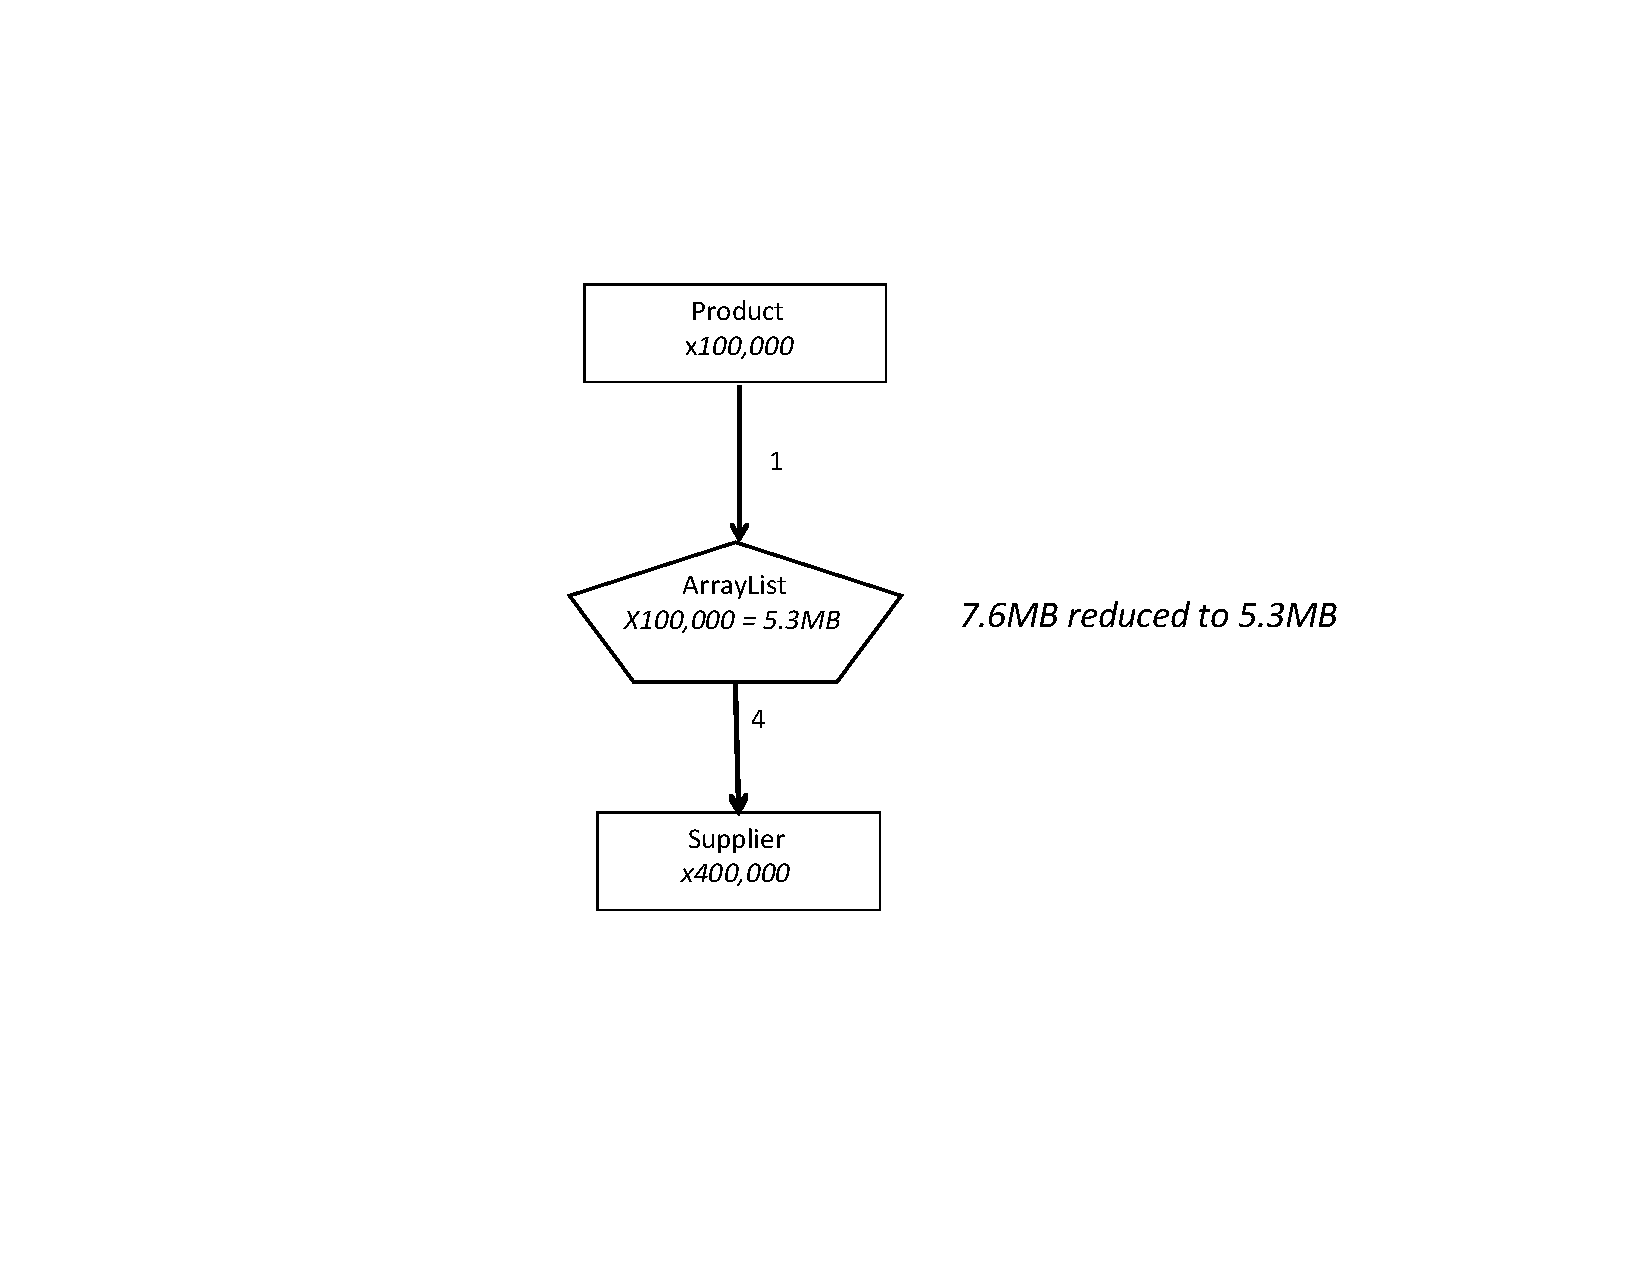
\includegraphics[width=.80\textwidth]{part1/Figures/collections/trimmed-product.pdf}
 \caption{The relationship between \class{Product}s and \class{Supplier}s after
 all of the
 \class{ArrayLists} have been trimmed by calling the \code{trimToSize} method.}
  \label{fig:trimmed-product}
\end{figure}
 
\class{HashSet}s and \class{HashMap}s do not have \code{trimToSize}
methods, but it is possible to set their initial capacity at construction time.
The capacity is actually not the number of elements the collection is
expected to hold. It specifies instead the number of hash buckets, that is, the
number of slots in the array. It is automatically rounded up to the
nearest power of two. Hash-based collections always require some excess capacity to reduce the
likelihood of collisions. In addition, if the collection does grow and the
array needs to be reallocated, there will be the expense of
rehashing the entries. The load factor, by default .75, determines the
maximum number of elements in the collection, relative to the size of the array,
before a larger array needs to be allocated. Therefore, it is important to take
the load factor into account when setting capacity. For example, a default
\class{HashMap} with capacity of 16 can hold a maximum of 12 elements
before needing to allocate a larger array. 
%so that you leave enough headroom

\autoref{tab:small-collections-minimum-samples} gives a sense of the savings you can achieve
for some common small collections by setting the capacity to the minimum.
\autoref{tab:small-collections-minimum-fixed-var} shows the breakdown into fixed and variable costs for some
minimally-sized collections. You can see, compared to \autoref{tab:small-collections-default}, 
how minimal sizing reduces the fixed cost.

An \class{ArrayList}, \class{HashMap}, or \class{HashSet}
will not automatically reduce the size of its array when elements are removed,
or when the collection is cleared.

%However, before changing the initial capacity, you should
%ask yourself whether using a \class{HashSet} or \class{HashMap} is a
%wise decision in the first place. If you are going to end up with many
%collections with fewer than 16 elements, perhaps there is a more
% memory-efficient solution, like \class{ArrayList}.
  
%A \class{LinkedList} is another alternative for small collections, and are
%better than \class{ArrayLists} if the collections are changing a lot. The
%24 byte per-entry cost is larger, but there is no element array, and only one
%extra entry, which is a sentinal.

\section{Avoiding Empty Collections}

Maintaining a large number of empty collections is another common problem that
leads to memory bloat. Empty collection problems are generally caused by eager
initialization, that is, by allocating collections before they are actually
needed. You might think that eager initialization would not be a big
problem, since entries will be added eventually. However, it's common to
find large numbers of collections that remain empty throughout an execution.

Making matters worse, the standard collections
allocate their internal objects in an eager fashion. For example,
\class{ArrayList} allocates its internal array before any
entries are inserted, and \class{LinkedList} always allocates a sentinel
entry. As a result, every empty collection takes two or more objects, as shown
in \autoref{fig:inside-empty}.
This is true even if you allocate the collection with the minimum possible
capacity.
Therefore, the smallest empty collections are still quite large. For example,
a zero-capacity \class{ArrayList} requires 40 bytes.
\autoref{tab:empty-collection-costs} shows the sizes for some common collection classes
when empty. 

%a zero-sized \class{ArrayList}
%consumes 40 bytes, the smallest \class{HashMap} takes 64 bytes, and the
% smallest \class{HashSet} takes 80 bytes. Table 

%A quick look inside the empty collections show that they
%are not all that empty! 


 \begin{figure}
  \centering
 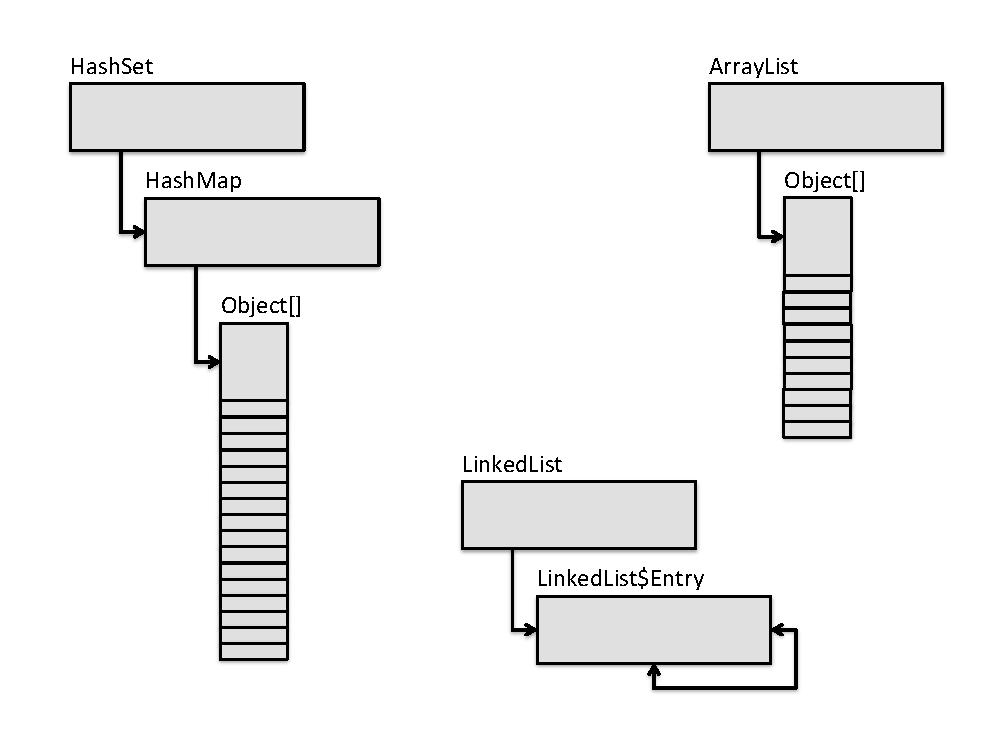
\includegraphics[width=.80\textwidth]{part1/Figures/collections/inside-empty.pdf}
  \caption{The internal structure of three empty collections. Each
  requires at least two objects, before any entries are added.}
  \label{fig:inside-empty}
\end{figure}

\begin{table}
\centering
 		\begin{tabular}{lcc}
 		\toprule
	 	 Collection & \multicolumn{2}{c}{Size in bytes} \\
	 	 & default capacity & minimum capacity \\
	 	 \midrule
	 	ArrayList & 80 & 40 \\
 		LinkedList & 48 & 48 \\
 		HashMap & 120 & 56 \\
 		HashSet & 136 & 72 \\
	 	\bottomrule
	 	\end{tabular}
	\caption{Size of empty collections, for some common
	collection classes.
	Empty collections require a lot of space, even when initialized to the smallest
	possible capacity.}
	\label{tab:empty-collection-costs}
\end{table}

\paragraph{Example} Suppose the relationship
in Figure~\ref{fig:trimmed-product} is initialized by the code:
%\begin{shortlisting}
%List<Product> products;
%int numProducts;
%..
%public void initAlternateSupplierRelationship() {
%	..
%	for (int i = 0; i < numProducts; i++) {
%    	Product product = products.get(i);
%		product.alternateSuppliers = 
%                           new ArrayList<Supplier>();
%    }
%}
%\end{shortlisting}

\begin{shortlisting} 
class Product {
	.. 
	ArrayList<Supplier> alternateSuppliers;
	..
	public Product() {
		..
		// Allocate the collection in advance
		alternateSuppliers = new ArrayList<Suppliers>();
		..
	}
}
\end{shortlisting}
Initially, each product allocates an empty \class{ArrayList} for alternate
suppliers, so there are 100,000 empty \class{ArrayLists} before any
\class{Supplier}s are inserted. As the alternate suppliers are populated, many
of these \class{ArrayLists} will become non-empty, but it is likely that a good
number of products have no alternate suppliers. If 25\% of the products have no
alternate suppliers, there will be 25,000 empty \class{ArrayLists}, which consume
about 1MB even after calling \code{trimToSize}.
Figure~\ref{fig:empty-array} shows the entity-collection
diagram after removing 25,000 empty alternate supplier \class{ArrayList}s.
The diagram now shows only 75,000 alternate supplier \class{ArrayList}s,
since there are no more empty \class{ArrayList}s. We therefore adjust the
average fanout in and out of \class{ArrayList} to .75 and 5.33, respectively.
\begin{figure}
  \centering
 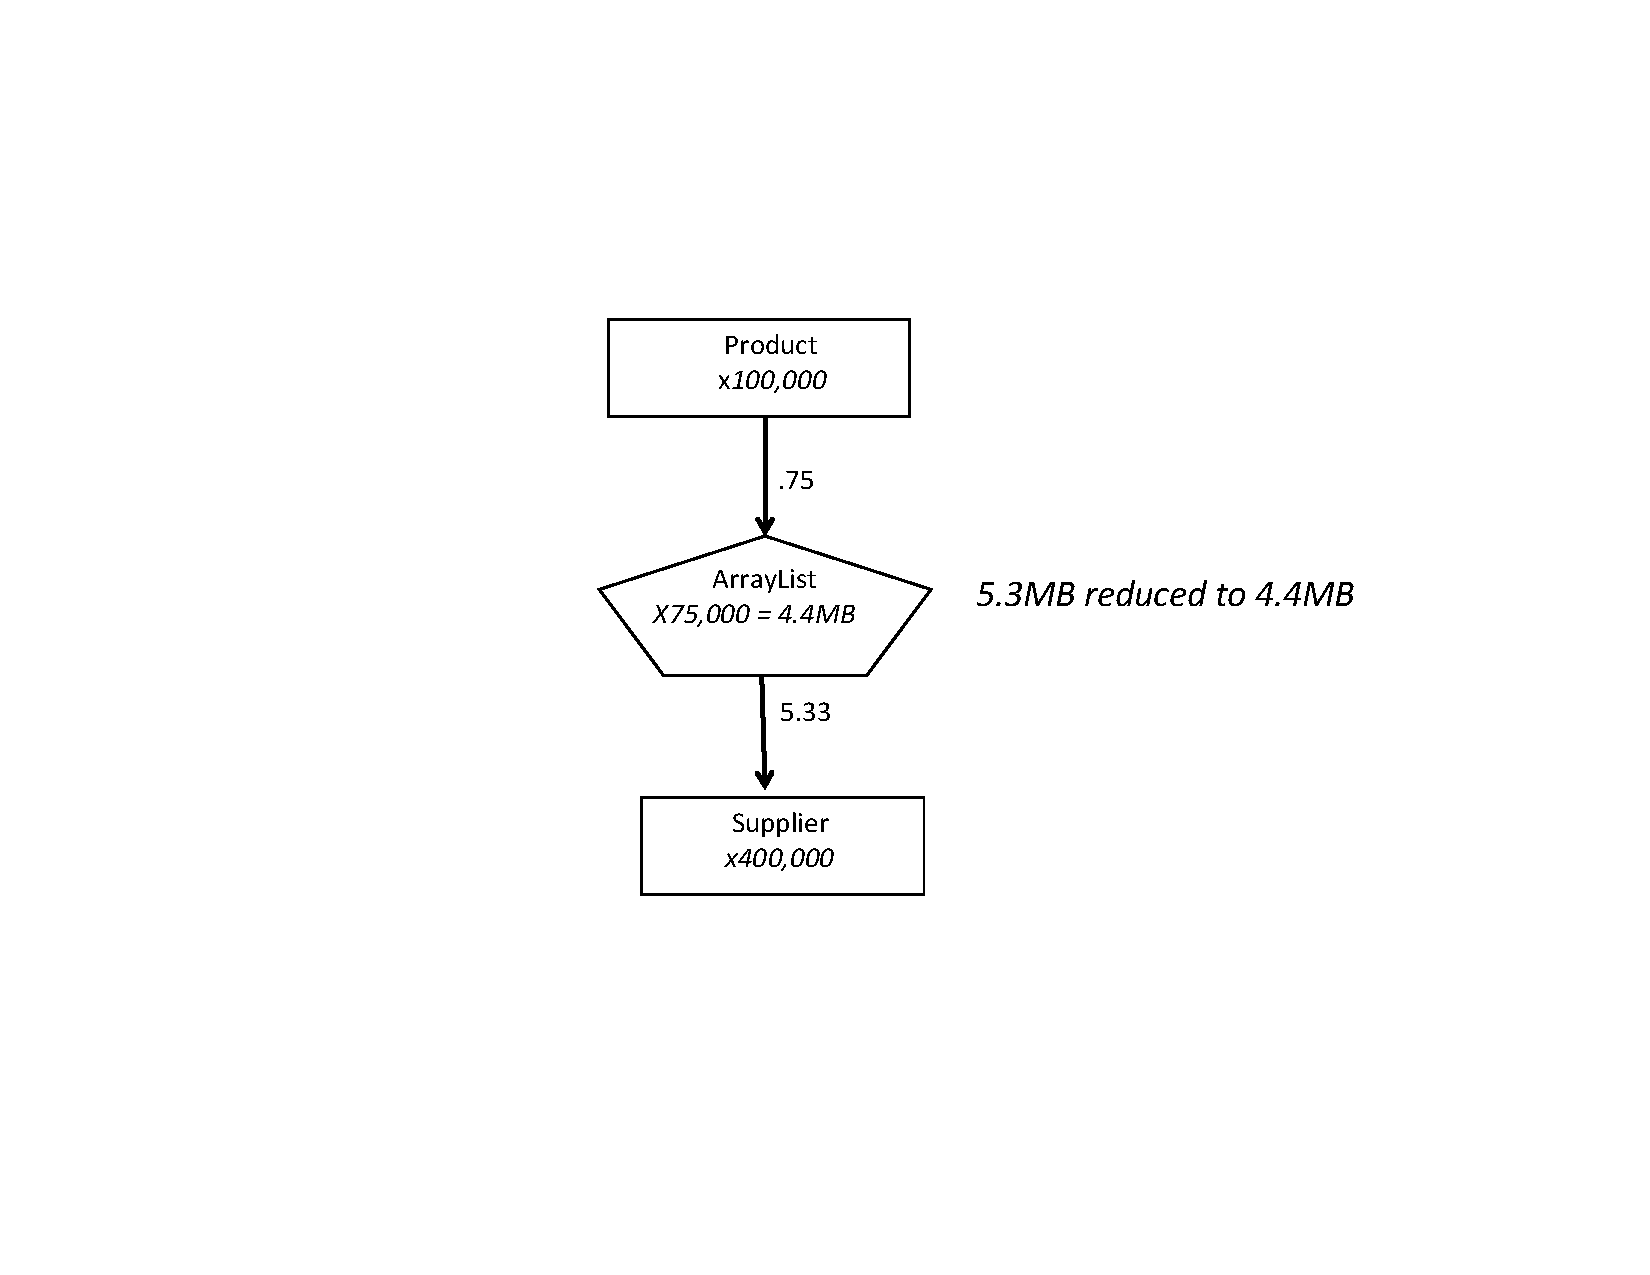
\includegraphics[width=.80\textwidth]{part1/Figures/collections/empty-product.pdf}
 \caption{The relationship between \class{Product}s and \class{Supplier}s,
  with no empty \class{ArrayLists}.}
  \label{fig:empty-array}
\end{figure}
 
 \paragraph{Lazy allocation} Delaying allocation is the way to
 avoid creating lots of empty collections.
 That is, instead of initializing all of the collections that you think you
 may need, allocate them on demand. 
 One approach is simply to leave collection fields null
 until needed. However, this requires extra checking code whenever you
 access these fields, to avoid \code{NullPointerException}s.
 
For many applications, the abstract
\class{Collections} class provides a better solution. You can initialize
collection fields to point to shared, immutable empty collections, using the
static methods \code{emptySet()}, \code{emptyList()}, and \code{emptyMap()}
\footnote{Static constants EMPTY\_SET, EMPTY\_LIST, and EMPTY\_MAP provide a similar capability,
without the type safety of generics.}.
The following code
maps all products to a single, immutable, empty list of suppliers, so that no
empty \class{ArrayLists} are created:

\begin{shortlisting}
class Product {
	.. 
	List<Supplier> alternateSuppliers;
	..
	public Product() {
		..
		// Initialize to a shared, static collection
		alternateSuppliers = Collections.emptyList();
		..
	}
}
\end{shortlisting}

This initialization avoids the need to check whether an \class{ArrayList}
exists at every use. The size method, iterators, and other access functions
work as in any other collection.
However, you have to be careful not to let any references to these static empty
collections escape their immediate context. If you do give out a reference, 
then there is no way to update this reference once an actual collection is
allocated. Instead, you can provide access and update methods to the relationship,
so that the implementation remains hidden.
You will also need to code to interfaces, delaying the use of a concrete class
until a collections is actually allocated. In this example, \code{Product}
declares a \code{List} of suppliers, so that it can point to either the shared
empty list, or to an \class{ArrayList} once it's populated.
This is, of course, a good practice in general, so that the implementation can
be easily changed later.

If lazy allocation is not a good option for your application, then
right-sizing collections, at initialization time or after loading is
completed, will still make a difference for empty collections.

%\section{Fixed Size Collections}
%
%Java collections can grow to be
%arbitrarily big, but this functionality comes at a cost.
%Collections include wrapper objects, and 
%may be sized with extra growth room. If
%you know that the size of a collection is fixed, having the ability to expand
%the collection is unnecessary, and it is better to choose a cheaper
% alternative.
%In fact, often you can use a
%simple Java array, and not use a collection at all.  
%
%In our example, alternate suppliers are stored in an
% \class{ArrayList}, which inside is a
%wrapper pointing to an array of \class{Suppliers}.  If we assume that
%every product has at most four alternate suppliers, then  it isn't 
%necessary to store these in an \class{ArrayList} --- a simple array will do.
%Eliminating the \class{ArrayList} object removes 24 bytes per
%product, but we have to add 4 bytes to each \class{Product} to store the number
%of alternate suppliers. The total savings is 1.43MB for 75,000 products:
%\begin{shortlisting} 
%class Product {
%	String sku;
%	String name;
%	.. 
%	int numAlternateSuppliers;
%	Supplier[4] alternateSuppliers;
%}
%\end{shortlisting}
 

%\begin{figure}
 % \centering
% 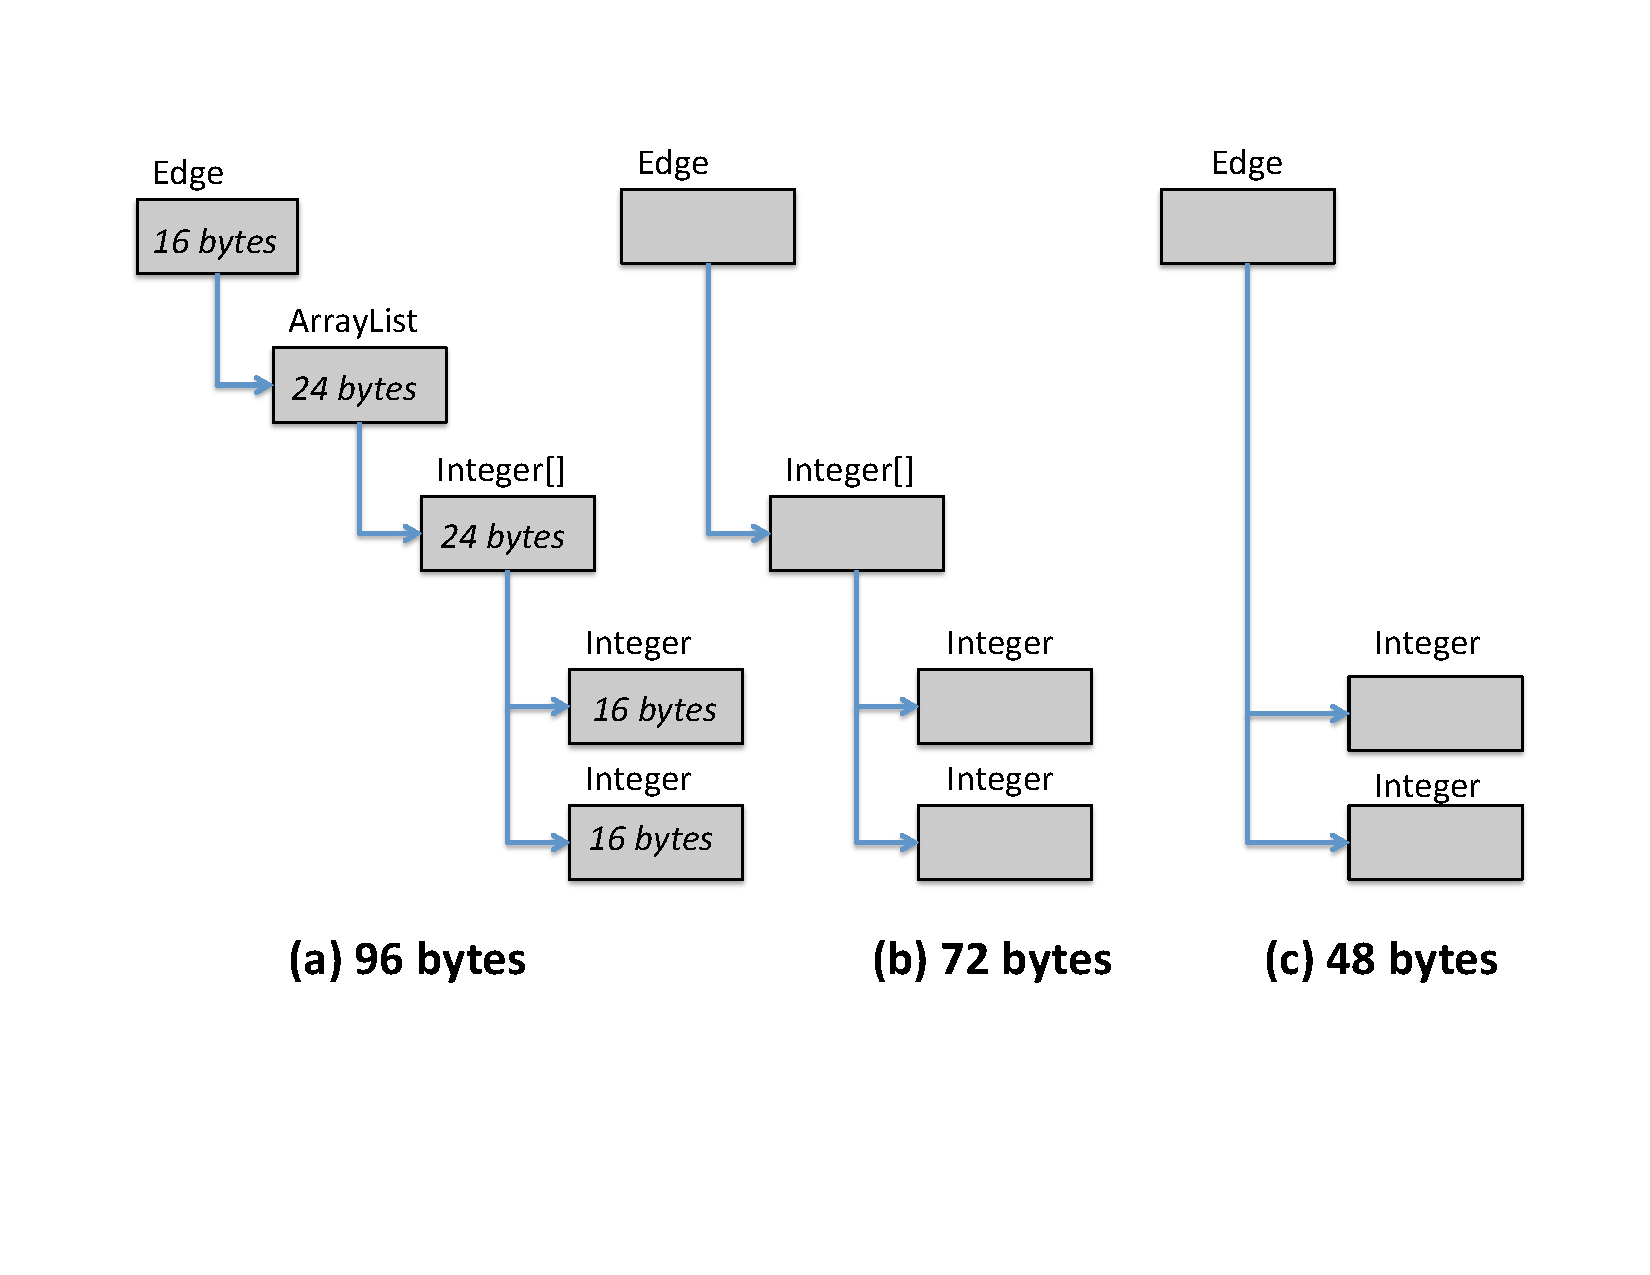
\includegraphics[width=.80\textwidth]{part1/Figures/collections/Edges.pdf}
%  \caption{(a) An \class{Edge} has 96 bytes. (b) Replacing the
%  \class{ArrayList} by an array eliminates 24 bytes. (c) Inlining the array
%  eliminates another 24 bytes.}
%  \label{fig:edges}
%\end{figure}
%This is an example of choosing an overly-general collection. In
%this situation, you don't need a collection at all. Using \class{ArrayList}
%for storing fixed- or bounded-size arrays is a
%common practice that can be easily avoided.
%
%There is one final optimization that can be performed on the \class{Product}
%class. Namely, making the four alternate suppliers into fields of
%\class{Product} instead of elements of an array. This optimization
% a 32 byte array object for 75,000 products, while adding three additional
% fields to the \class{Product} for 100,000 objects, saving another 1.1MB in
% total:
%\begin{shortlisting}
%class Product {
%	String sku;
%	String name;
%	.. 
%	Supplier alternateSupplier1;
%	Supplier alternateSupplier2;
%	Supplier alternateSupplier3;
%	Supplier alternateSupplier4;
%}
%\end{shortlisting}
%
%This representation is very similiar to the original \class{Product} class in
%section~\ref{sec:rarely-used} where there is one alternate suppler field, and
%here there are four. Taking all of the optimizations 
%together, we have gone from the initial \class{HashSet} representation
%of 22.1MB in Section~\ref{section:choosing-collection} to the in-lined field
%representation of 1.86MB. 


\section{Hybrid Representations}
\subsection{Mostly-small collections}
It is often the case that the collections used in a relationship
are not of uniform size. There often are many collections that are small and fewer that are
very big.  It's reasonable to use an expensive collection like \class{HashSet}
for the big collections, but then the small collections pay the price. One way
to handle this problem is to use a hybrid representation. For example, you can
use \class{ArrayList}s for smaller collections, and \class{HashSet}s for larger
collections. 

One catch is that you usually will not know in advance which collections in the
relationship will end up being small and which will grow to be large. Therefore
one or more conversion operations will be necessary at some point if a
collection grows large enough. 

Returning to our original example, let's suppose that our average of 4 alternate
suppliers per product is distributed as follows: 25\% of products have no
alternate suppliers, 25\% have one alternate supplier, the next 25\% have
between 2 and 6, averaging 3 each, and the remaining 25\% have an
average of 12 each.
Let's also assume that we do in fact need to guarantee uniqueness in the data
model. The code for the \class{Product} class is shown below. As in the case of
lazy allocation, we'll need to hide access to the collections behind
accessor and update methods. 

\begin{shortlisting} 
public class Product {

	// Threshold for switching to HashSet
	private static final int arrayListMax = 6;
	.. 
	protected Collection<Supplier> alternateSuppliers;
	..
	public Product() {
		..
		// Initialize to a shared, empty collection
		alternateSuppliers = Collections.emptyList();
		..
	}
	
	public void addAlternateSupplier(Supplier supplier) {
		int numSuppliers = alternateSuppliers.size();
		if (numSuppliers == 0) {
			// Create a singleton list
			alternateSuppliers = 
				Collections.singletonList(supplier);
			return;
		}
		if (!(alternateSuppliers instanceof HashSet)) {
			// Uniqueness check for non-HashSet cases
			if (alternateSuppliers.contains(supplier)) {
				return;
			}
			if (numSuppliers == 1 && 
			 	!(alternateSuppliers instanceof ArrayList)) {
			 	// Convert to ArrayList
			 	alternateSuppliers = 
			 		new ArrayList<Supplier>(alternateSuppliers);
			}
			else if (numSuppliers == arrayListMax) {
				// Convert to HashSet
			 	alternateSuppliers = 
			 		new HashSet<Supplier>(alternateSuppliers);
			}
		}
		// Add supplier
		alternateSuppliers.add(supplier);
	}
	..
}
\end{shortlisting}

\paragraph{Singleton collections}
The standard library class \class{Collections} provides
\emph{singleton collections} that hold one element each.
These use much
less memory than their more general counterparts.
A singleton list and set take only 16 bytes each. Singleton collections
can be created via factory methods in \class{Collections}. In our
example, we first initialize the relationship with a shared
reference to a static empty set, in case there are no alternate suppliers. The method
\code{addAlternateSupplier} creates a singleton set to hold the first alternate supplier, if one is added. 
The singleton collections are immutable, in other words, they cannot be modified once they are
initialized. In your application, though, if you expect there to be
deletions and they are infrequent, it's easy enough to write code that simply
deletes the singleton collection until it's needed again.

\paragraph{Converting to larger representations}
If an additional alternate supplier is added, \code{addAlternateSupplier}
replaces the singleton list with an \class{ArrayList}. We can choose a
threshhold, say six entries, to be the maximum number of alternate
suppliers the \class{ArrayList} representation should hold.  If more
alternate suppliers are added beyond that, the representation is switched
to the more costly \class{HashSet}.
For the singleton and \class{ArrayList} representations, we need to check
uniqueness, and we use the \code{contains} method to do so. For \class{HashSet},
we can rely instead on
\class{HashSet}'s built-in uniqueness checking. 

%The method \code{addAlternateSupplier} adds the supplier to the array if the
%size is less than the threshold, otherwise, it adds the supplier to the
% \class{HashSet}.
%It allocates the alternate supplier array and \class{HashSet} 
%only if and when it is needed, to avoid wasting space with empty collections
%when there are no or only a few alternate suppliers.

Implementing hybrid representations is more complicated than just using one
type of collection for a relationship. However, it can save significant space in some
cases. In our example, an implementation that uses a
\code{HashSet} (minimally sized) and shares a single empty collection would
spend 18.9MB on collections overhead. The hybrid representation would reduce
that to 11.6MB, a 38\% savings. 
%This can save even more space.

\subsection{Load vs. use scenarios}

Another scenario where you can benefit from multiple representations is when you
have a distinct load phase followed by a phase where you only need read access
to the data. If your application requires more expensive functionality at load
time, such as uniqueness checking, frequent deletions, or maintenance of
insertion order, and you can afford a higher footprint during that phase, a
representation such as \class{HashSet} or \class{LinkedList} can be a simple
solution. Once loading is complete, you can make a second pass over
the data and replace the relationship with a more compact collection, such
as \code{ArrayList}. Since the cardinality of each collection is known in
advance, it is easy to allocate each \code{ArrayList} to the right size.

Depending on how much extra coding and maintenance you are willing to do, you
can further optimize by using arrays rather than collections, since you know the
size of each array in advance. This can save you
the cost of the \code{ArrayList} wrapper, or 24 bytes per collection. In
general we do not encourage coding your own collection functionality unless
you absolutely have to.  Most of the complexity of collection
behavior is in the update functionality, however. These collections are
readonly, which should make coding simpler.

Another alternative, if you would like to guarantee that the use-time
collections are readonly, is to use an immutable collection class, such as
one from the Guava open source framework. See
\autoref{sec:immutable-collections} for details.

The fastutil open source framework provides one more
solution for certain cases. Its \code{ObjectArraySet} class is one of the few
collection classes from any framework that uses less memory than the standard \code{ArrayList}.  Its
fixed cost is 32 bytes vs. the \code{ArrayList}'s 40.  It provides set behavior
backed by a simple array. Its only caveat is that its \code{contains} function
uses a linear search, which will be slow for a large set. 

\section{Special-purpose Collections}

\subsection{Immutable}
\label{sec:immutable-collections}

\subsection{Unmodifiable}
\label{sec:unmodifiable-collections}

\subsection{Synchronized}
\label{sec:synchronized-collections}

\begin{table}
\centering
 		\begin{tabular}{l||r||r||rrl}
 		\toprule
	 	 Collection & with 1 entry & with 4 entries &
	 	 \multicolumn{3}{c}{with n entries}\\
	 	 & & & fixed & variable & comments \\
	 	 \midrule
	 	\multicolumn{5}{l}{Collections statics:} \\
	 	\midrule
	 	SingletonSet &  16 & - & 16 & - &  \\
	 	SingletonList & 16 & - & 16 & - &  \\
	 	SingletonMap &  40 & - & 40 & - &  \\
	 	\midrule
	 	UnmodifiableList & - & - & 16 & - & add'l cost \\
	 	UnmodifiableSet & - & - & 16 & - & add'l cost \\
	 	UnmodifiableMap & - & - & 24 & - & add'l cost \\
	 	\midrule
	 	SynchronizedList & - & - & 24  & - & add'l cost \\	 	
	 	SynchronizedSet & - & - & 16  & - & add'l cost \\	 	
	 	SynchronizedMap & - & - & 32  & - & add'l cost \\	 	
	 	\midrule
	 	\multicolumn{5}{l}{Guava:} \\
	 	\midrule
	 	ImmutableList & 40 & 56 & 36 \footnotemark[1] & 4 & for any n \\
	 	ImmutableSet & 64 & 96 & 64 \footnotemark[2] & 8 & for any n \\
	 	ImmutableSortedSet & 40 & 56 & 36 \footnotemark[1] & 4 & for any n \\
	 	 \midrule
	 	\multicolumn{5}{l}{fastutil:} \\
	 	\midrule
	 	ObjectArraySet & 32 & 48 & 28 \footnotemark[1] & 4
	 	& for any n \\
	 	\midrule
	 	\multicolumn{5}{l}{Java 1 collections:} \\
	 	\midrule
	 	Vector & 40 & 56 & 36 \footnotemark[1]  & 4 & for any n\\ 	
	 	\bottomrule
	 	\end{tabular}
	 	
	\caption{A sampling of special-purpose collections. When it applies, costs
	shown are when minimally sized.}
	\label{tab:specialized-collections-small}
\end{table}

\footnotetext[1]{Round total cost up to nearest 8 bytes.}
\footnotetext[2]{Round total cost up to nearest 16 bytes.}

\FloatBarrier

\section{Summary}

Collections used to represent relationships often result in many small
collection instances. The cost is dominated by fixed-size
overhead; variable overhead matters as well. To mitigate high memory costs
for relationships:
%implemented with collections:
\begin{itemize}
  \item Choose the most memory-efficient collection for the job at hand. For
  example, when collections have at most a few elements in them, you
  don't need expensive functionality like hashing. In
  order to choose, first ask some questions about the relationship:
  \begin{itemize}
    \item What operations will be performed? Will there be deletions,
    insertions, uniqueness checks?
    \item What's the cardinality? Is it uniformly
    distributed across the instances, or are there mostly very small
    collections?
    \item Is there a distinct load phase, after which the relationship no
    longer changes?
  \end{itemize}
  \item Make sure collections are properly sized. If you know that a collection
  will not grow any more, then there is no reason to maintain extra room for
  growth.
  \item Avoid lots of empty collections. You can postpone creating collections
  until they are needed.
 \item When the size distribution is not uniform, it is sometimes reasonable to
 use a hybrid representation that adapts to the data. If there are
 distinct load vs. use phases, a different representation
 for each phase can be a good solution.
 \item Some special-purpose collections can help save space, such as
 \code{SingletonSet}. Others are not
 designed for use at a small scale. Make sure the
 behavior is worth the added cost.
\end{itemize}
Knowing which relationships and collections in your application are the most
important and need to scale is key to applying these optimizations effectively.  





\chapter{Large Collection Structures}
%\chapter{Large Structures for Accessing Data}
\label{chapter:tables-indexes}

In a relational database system, data is neatly organized for you into tables.
While you may suggest a few fields to index, the structures that
allow you to access your data are taken care of for you.  In object-oriented
programming languages you have more freedom. You have a sea of interconnected
objects, and you are responsible for designing the structures that are the entry
points into various groupings of these objects.
In this chapter we look at the memory considerations when
designing large structures for accessing your
data. We'll
look briefly at large collections that just gather data in one place, such as a
list of all the objects of one type. The bulk of the chapter is about
indexes, also known as maps, that let you look up data by value. We'll first look at the costs of large collections,
and at ways to keep them to a minimum for the task at hand. In the second half
of the chapter we'll look at the cost tradeoffs when you need to
design more complex access structures made of multiple levels of collections.  


%Collections, especially large collections, are your
%main tool.
%Maps are the main
%implementation mechanism in these structures \footnote{We use the term map to
%mean a Java collection class, and the term index to describe the general
%functionality.}.

%Large collections, like much else in Java, can
%take up a lot of memory, unless you choose and configure them carefully. 

%, it's easy to create very expensive designs. 


%As we saw in the previous chapter, the
%overhead of different collection choices varies quite a bit. The costs for
%large collections play out somewhat differently than in smaller ones. In
%large collections, whether lists, sets, or maps, the main issue is the
%incremental cost of each new element. This is because the fixed cost of the
%collection is insignificant once the collection is above a certain size.  



%We walk
%through a sample analysis, comparing three alternative designs.


% Here we look at how the costs work out for large collections,
%and what choices are available
%including in open source frameworks if you are able to use these in your
% system.  We'll also look at some
%common special cases. If your requirements fit into one of these cases, there
%are less expensive solutions available. 


%In any large collection, the main
%issue is how to keep down the cost of adding an element. The fixed
%cost of the collection becomes insignificant once the collection is above a
%certain size.  We look at ways to keep these variable costs down: by
%carefully choosing the right collection for the situation; by
%recognizing some special cases that enable some optimizations; and by using
%some of the open source collection classes if they are available to you
%(rephrase all of this is what the reader can do, not as a roadmap).


\section{Large Collections}
\label{sec:large-collections}

Just as with small collections, choosing the right collection for the task
can make a big difference in the memory overhead of large collections.  Suppose
you need to maintain a collection of all the orders processed for the day.  At
the end of the day these orders are posted in bulk to a remote database. The orders
contain their own timestamps, so we don't really care about maintaining the
sequence in which they were received. Figure~\ref{} compares an implementation
using \class{ArrayList} with one using \class{HashSet}. As with small
collections, if we don't need the uniqueness checking or some of the
other features of \class{HashSet}, then we are clearly much better off with \class{ArrayList}.

In larger collections, the variable overhead --- the cost each element incurs
--- determines the cost of the collection. That's because as a collection grows its fixed overhead,
such as wrapper objects and array headers, becomes insignificant. For example,
in an \class{ArrayList} with 100 elements, the fixed cost is only 9\% of the total. With 1000
elements, it falls to 0.1\%.  The difference in size in the above example is
pretty dramatic, more than 7:1.  That reflects the difference in the variable overheads of the two
collection classes. Like much else in Java, variable overheads in large
collections can take up a surprising amount of memory if you are not careful.
%With small collections we need to concern
%ourselves with both fixed and variable costs, for large collections we
%need only look at variable costs. 
As a general rule,
the variable overhead of array-based collections, like \class{ArrayList} is much lower than that of 
entry-based collections where a new entry
object is allocated for each element in the collection. You may have noticed
that most of the collections in the standard collection library are entry-based,
including \class{HashMap}, \class{HashSet}, \class{LinkedList}, and \class{TreeMap}. Table~\ref{} shows a
comparison of variable costs for the most commonly used classes from the standard collections library, 
along with a sampling from open source libraries.


%You may have noticed that in our current example,
%there is a much bigger difference between the two implementations than there
%was in Section~\ref{}, where we compared the same two collection classes in a
%design that had small collections.  For small collections, the fixed costs are
%a larger part of the overhead, whereas here it's only the differences in
%variable costs that matter.  

\paragraph{Excess Capacity}

As we saw in the previous chapter, many collection
classes allocate excess capacity for performance reasons, mainly to accomodate
growth. One difference between small and large collections is the way
excess capacity is computed.  In the very smallest collections, excess capacity
comes from the initial capacity being too large. In contrast, as a collection
grows larger, the amount of spare capacity allocated is proportional to the
number of elements. For example, whenever an \class{ArrayList} needs
more space, it allocates an array that is 50\% larger than its current
size; \class{HashMap} doubles the number of buckets when the number
of elements reaches a user-specified load factor. So for any collection that's
grown beyond its initial size, you can 
think of spare capacity as part of the variable cost.
If an \class{ArrayList} is 1/3 spare capacity, then every
element really costs 6 bytes, rather than the 4 bytes for the array slot that
holds the pointer.

Collections grow in jumps, which makes predicting the size of a collection a
little tricky.  For that reason, Table\ref{} shows
a range of variable costs for each collection.  You can use the minimum
number if you expect no spare capacity, or in the case of hashtable-based maps
and sets, no spare capacity beyond what is required for reasonable operation.
The maximum number gives you a worst case, if you added just that one extra element that caused
the jump. Slightly less than the midpoint of the range will give you an estimate of the
variable cost if the most recently allocated spare capacity is half occupied.
Again, the table only applies to collections once they have grown beyond their
initial size.
% For tiny
%collections, the excess capacity can cost much more per element, as we saw in
%the previous chapter.

Solutions for reducing excess capacity for larger collections are the same as
for small collections. If you can estimate the number of elements in advance,
you can try to size the collection carefully when you create it.  If your data structure has a
distinct load phase, and the collection has a \code{trimToFit()} call, you can
trim the size of the collection after the load phase is complete. In hash-based collections, such as
\class{HashMap} and \class{HashSet}, excess capacity is needed to reduce the
likelihood of collisions, so it's important to leave headroom for this
purpose. The default load factor is usually a pretty good guide. 

Excess capacity isn't much of an issue for collections like
\class{HashMap} and \class{HashSet}, where the bulk of the overhead is from the entry objects.
For larger array-based collections, excess capacity can be a more significant
part of the overhead, though it's relative to a more efficient representation in the
first place. 

%Notice that for large collections, the issue of excess capacity is not as
%serious as that for designs with many tiny collections, like those we saw
%in the previous chapter, where the initial 
%capacity is so much larger than the number of elements stored.

\paragraph{Array-based Hash Maps and Hash Sets}

There are two primary ways that hash tables are implemented. Most of the maps and sets
in the standard libraries use a technique known as \emph{chaining} (also
known as open hashing). Figure~\ref{} in the previous chapter shows a typical
implementation. There is a separate entry object for element in the collection.
Each entry object points to a key and a value, and may contain
additional information such as a cached hash code. There is a linked list of
entry objects for each hash bucket.

The other main technique is known as \emph{open addressing} (for added
confusion, it is also known as closed hashing).  In this technique,
keys, values, and other information are stored directly in
arrays. These are usually parallel arrays, though some implementations
use a single array and interleave different kinds of information in
successive slots. Chains of entries that map to the same bucket are threaded through the arrays.
Figure~\ref{} shows a typical implementation. There are many variations in
practice.

Generally speaking, for larger collections, open addressing hash tables use less
memory --- at least in Java, where the cost of an entry object is so high. 
fastutil and Trove are examples of open source frameworks that provide open
addressing maps and sets that save space. The sets in these frameworks
save even more space for a different reason: they are specialized for the task,
rather than delegating their work to a more general map. So unlike in the Java
standard libraries, you are paying only for a value, not a key and value, per
entry.

Since open addressing hash tables usually use less memory, why do so many hash
table libraries use chaining? Generally speaking, hash tables based
on chaining are much simpler to implement. More importantly, there
are performance differences between the two approaches, though there is no easy
rule about one always being faster than the other. For your
own system, if performance of your collections is critical it can be worth doing
some timings first.  Keep in mind that in many systems, the amount of
time spent in hash table lookups is a small fraction of the total execution time to begin with. 

Another thing to be aware of in open addressing implementations is that the
need for excess capacity will reduce the space savings to a greater
extent than in open chaining implementations. So it's important to look at the
entire variable cost when making decisions on which framework to use (see Table
~\ref{}).  For example, fastutil's object to object open addressing
hash map maintains only 9 bytes of data for each element, compared to the standard
\class{HashMap}'s 28. When you add in the greater cost of excess capacity that
difference is reduced to approximately 1:2.  <or example here instead, with absolute numbers>

\paragraph{Sharing the Costs in Entry-based Collections}

Some alternative frameworks provide another approach to reducing space in
entry-based collections. The idea is that your objects become
the collection's entry objects, thus saving a delegation overhead. The downside
is that they transfer some of the work of maintaining the collection to your code.
One example is in the Apache Commons framework, which lets you subclass its map
and map entries. If you have a key with two fields, for example, you would
normally have to wrap those fields into a key object. Now 
you could include those fields in a custom map entry instead, and save a
delegation cost. <figure here?>  This introduces a reliability and maintenance
problem, however, since it relies on subclassing a fairly complex class. You must now make sure
your code doesn't break anything in current and future versions of Commons's
hash map implementation.

A simpler approach is taken by Trove's linked list. If you have a class whose
objects are to be stored in a linked list, your class can implement the
\class{TLinkable} interface. Your class would provide the chaining, and
again, save the cost of a separate entry object.  Some restrictions are
necessary in order for this to work: no instance of your class can
be a member of more than one linked list simultaneously, nor appear more than
once in the same list. In addition, your class must now include
pointer fields, which increase the cost of these instances when they are
not stored in a list.

\section{Identity Maps}
The Java standard library does provide one hash map class that uses an open
addressing implementation. The \class{IdentityMap} class can save you space
if you have the need for a large map that fits its requirements.  The idea is that
it uses the identity of the key object, 
rather than its contents for comparisons. In
other words, it uses \code{==} against the key your provide, rather than the
\code{.equals()} method. This breaks the \class{Map} contract, but there are a
number of applications where this doesn't matter.

Suppose I want to associate additional information with each product.  Using a
standard map, I could map the product's unique key, say SKU, 



\section{Maps with Scalar Keys or Values}

\section{Multikey Maps. Example: Evaluating Three Alternative Designs}

\section{Concurrency and Multilevel Indexes}

\section{Multivalue Maps}

\section{Summary}




\chapter{Attribute Maps and Dynamic Records}

\chapter{Additional Collection Behaviors}
\label{chapter:additional-collection-behaviors}

%\chapter{The Cost of Java Collections}

It is not unusual for a Java application to have hundreds of thousands, even
millions, of collections. To get this many collections, ollections are
nested in other collections, sometimes three to four levels deep. Collection
infrastructure is pure overhead, so using too many or choosing expensive
collections can lead to a huge amount of bloat. This chapter 
analyzes the memory cost of the four most common, representative collections: 
\class{ArrayList}, \class{LinkdedList}, \class{HashSet} and \class{HashMap}.

%What the different libraries are. Where we take our overhead costs from. 
%What alternative libraries are out there.
%%And finally, some of these specialized collections are worthwhile for their
%functionality, if not only for it�s footprint. The identity map is worthwhile
%for its footprint. Just some alternative collections. Like I said, the Apache
%can tell, at least from the code I�ve looked at. The Trove collections are great for footprint, 
%but we are not allowed to use them, at least from what I understand. Anything
%you work on that may go out, you really have to check specifically.   The
%opensource licensing stuff, it�s on a product by product basis. There�s a lot
%of collection class efforts Amino classes are aimed at concurrency, Javalution
%from Raytheon is for soft realtime, and externally on sourceforge, Cliff Click
%has some non-blocking collections. Actually, he claimed the footprint is good.
%I haven�t seen any studies on it. The best source of good collections I�ve
%seen are actually scattered around the IBM frameworks. Portal, Rational, just
%
%all over the company.


\section{Basic Java Collections and Their Costs}

Describe container object, entries and arrays, and each entry overhead. fDescribe fixed costs vs. 
per entry costs. Give the figures for empty collections.

And juust a quick look at the cost of the empty collections. What strikes me � 
these are the number from both \oracle and IBM. What strikes me is that the smallest number 
here is 48, so there�s certainly no single digit anything in Java, but 48 is a pretty high number 
for something that�s empty, if you are going to have a lot of them, and also, there�s a little
 bit of variation, both having to do with whether you�ve made the size default or not, and also 
 what kinds of collection class you are choosing.


Just a quick look at some of the default sizes. LinkedList, it�s not really applicable other 
than the fact � always comes with an extra entry as a sentinel, just to make the coding of 
LinkedList simpler, So you are actually paying 3 entry cost for a 2 element collection. 
ArrayLists, the default size is 10. For some reason, the latest J9, in these Harmony classes, 
which are open source, they�ve upped it to 12, and I�m not quite sure why they�ve done that. 
Actually that�s not really true. The default size initially for an empty collection is 0, 
so they�re still allocating the array with 0 size. Where as the \oracle and older JVM�s are always 
allocating 10 element collection. But on the Harmony classes, the new J9, after you add the first 
element, they jump it to 12.


\section{Example: HashSet}

HashSet actually doesn�t do any work itself, it delegates it HashMap. So there�s the cost of the 
HashSet, and now you have whatever the cost of HashMap is.  We talked about last week delegation 
costs can be pretty high, so you are paying an extra object overhead plus a pointer. 
HashMap itself actually a fairly expensive class also from a memory standpoint. It delegates its 
work to an array, sort of a necessity in Java, and it also has a number of bookkeeping fields, 
we will talk about in a minute. The thing is pretty hefty. On top of it, the default size of the
 array, if you don�t specify something is 16. So you get 16 size array, and this is all fixed 
 cost. Before we have even gotten to the cost of the actual entries in it. The way HashMap is 
 implemented, it is using open chaining, which means that each hashmap entry turns into a 
 hashmapentry object, similar to the treemap example last week. SO the end result is that HashSet 
 is a pretty poor choice if you have small sets. At least with its current implementation. 
 Obviously, it�s worth measuring here. And indeed the developer did, and was able to solve the 
 problem. Some other lessons in here about what the developers of hashset must have been thinking,
  and really for anyone who is developing a library of framework that is going to be used higher 
  up. Basically, they hardcoded in a lot of the assumptions about its expected usage.

The first assumption here is whether it was conscious or not, is that internal reuse is more 
important than having a low fixed cost, which means they didn�t really expect
to have a lot of ]small hashsets. If the thought it through, they probably thought that fixed 
cost doesn�t matter because you weren�t going to see a lot of these things. In fact, we see 
millions of these, and this is the kind of thing, we talked about last week, that low level 
libraries in particular, specialization is a good thing.  Or it can be a good thing, and reuse 
is sometimes a misplaced value in these kinds of cases.

In this case, the reuse has a fixed cost of 24 bytes per set, and this is based on 1.4.2, 
the J9 numbers are a bit higher. It also has a per entry cost because each hashmap entry is 
storing a key and a value, and hashset isn�t using both. It�s only using the key, it isn�t using 
the value. The value pointer is pointing to a constant. So the whole thing is over general than 
needed. HashMap is expensive just for HashMap. It could be much more specialized for HashSet. 
And we also have the default size of the array. The third problem is that hashmap has a bunch 
of bookkeeping fields in it, that really are rarely needed, and certainly not needed all together. 
It has a bunch of fields to keep different views of the hashmap that you might want. 
The map interface says that you can compute a collection of all the entries, all the keys, 
and all the values. And HashMAp caches all of those. So every HashMap, and every HashSet, is 
paying these three pointer costs, which is an extra 12 bytes. In fact, you rarely use all three 
together, and it�s not all that common to use even one of them.

The other thing is that the hashmap entry itself is storing a hashcode.
 It�s maintaining a hashcode, even though the most common cases are keys, 
 either strings, store their own hashcode. Or integers, where the hashcode computation
  is pretty trivial. So that�s also a misplaced optimization, and you have to ask the question. 
  Was this based on an empirical study, with possibly the wrong benchmarks, or was this based on 
  some assumptions? In this case, it was sort of another cautionary tale for library designers 
  of the danger of premature optimizations. 


\section{Summary}

Decisions programmer must make: which to use, how to model, how to manage;
Depends on scenario. E.g. concurrent use, load phase, use phase. Do you know how big to expect? 
 

So now some special cases in this. There are a lot of different uses of this, and one
 interesting things we�ve been learning, as we�ve been looking at all these case studies
  is that we�re really trying to think about why are people using collections, and what are
   they using them for? In the last example, we saw, they are using them to implement a map. 
   A fairly complicated map. In that first long example. 

People don�t do this until they have a problem. Don�t have tools. Either they don�t 
know things are this bad. It�s just a collection, just an integer. Or the tools are so hard to 
use, no easy way to do it until they have a crisis. 

The garbage collector is not the answer to this. Garbage collector�s realm is cleaning up 
temporaries. This is a problem of long lived-objects. The gc is not addressing these things at 
all. People have the assumption that the JIT, the garbage collector, things are magically being 
taken care of. There�s no footprint optimization being done in any commercial JITs. 

Because Java has a gc, they don�t give you the tools to do your own memory management, and these 
are the tools you need to figure out how big things are.

We�re making logical decisions, but Java is forcing us to manage it as physical things. Object
 oriented storage. Just how limited, you really hit it with the idea the GC is going to 
 everything for it, so there are no other tools for managing storage. Simplified java modeling 
 scheme � no unions, all the little tricks you have in C++ just don�t exist in Java. 

Model driven development, tools should give you the ability to choose the right 
implementation. The developer is interestedin the data model. UML to Java transformation 
should just do the work for you.

Just a summary of colllecitons.
There are really 2 classes of scaling issues. One is you have small nested collections, 
and you are paying the fixed cost of small collections, plus you may be paying per entry costs, 
if they have high per entry costs too for the small collections. The other case is the 
per-element costs of larger collections or nested collections, and any data delegation costs 
that those occur of the objects you store in them.

Just a little more about standard collections. The focus has been speed. Or supposedly it has 
been speed. It certainly hasn�t been footprint. There�s been very little attention given to that.
 I was a little surprised to see in the harmony classes. They harmony classes are the newest 
 classes for J9, version 6. They have been open sourced on Apache. I was surprised that Harmony,
  I thought this was great, they finally fixed some of this stuff, and I found that they actually
   increased the footprint in a couple of cases. They added an extra field to arraylist, they made 
   some of the sizes bigger. They cut the footprint in a number of cases too, but nothing 
   substantial. I think the more disturbing part here, is the fact that a lot of the assumptions 
   are hard wired. So there are not a lot of policy knobs to play with when you are coding to 
   these things, and that�s really a problem. 

Developers have a tough situation. Choosing the collections not always obvious what the choices
 are. Purpose, to raise the awareness. What kinds of things to think about, what to measure. 
 Not to think that things are cheap. And in this context of expensive implementations, 
 sometimes you do hit walls, and there�s nothing you can do. But sometimes you really can 
 fix a number of problems. There�s a lot of problems that have easy solutions. 
 Choosing the default size, lazily allocating collections that are most likely to be empty. 
 Picking a collection with less functionality if you don�t need the full functionality. 
 I strongly advise not writing your own collections, unless you really have search the company
  for something that will do the job, because it just introduces a whole other set of problems.

Implementing a cache, relationships, a nested map, attribute-value pairs etc � global 
optimizations. Study � what�s most of the heap?  Which kinds of database bulk storage 
optimizations would be appropriate?

%\chapter{Nested Collections}

WHere talk about per-entry costs?

Lists in Maps -- if phased, then make a big list; array list. 
If fixed, then can use a scalar map.
Scalar maps -- there are cheaper versions out there for integer maps.

Somewhere -- Lots of small strings; can be replaces by one big string and
offset/length into it. (THis is scalar data overhead..).



So that was all about small collections, and their problems. We kind of segwayed into the other 
half of the collection problem, which are collections that have high per entry costs. Typically 
large collections, but not always. Our design 3 really suffered from that. Basically, it 
has a high constant cost per entry. Just like our tree map did last week in the  health example. 
So each of these, just the per vertex and level cost here, is 48 bytes. It�s 28 bytes per enty 
in this hahsmap, and 20 for the pair objects.  It�s a constant cost that won�t be amortized.
 This is a theme that shows up in a lot of Java collections, in particular larger ones. 
 Just a quick look at the per entry costs.
They are fairly high other than for arraylists. HashMap and HashSet is 28 or  36. ArrayList 
is the lowest I�ve seen. and LinkedList is 24 for again, this is purely because there is a 
separate object in the collection, delegating to your object. And that doesn�t include the cost 
of any boxing you have to do on your side to introduce a pair class, or a cap int, or anything 
like that.  That could easily double some of these numbers.

So it�s pretty common to see that in large collections, like in example we just saw. Another case 
is when you have nested small to medium sized collections, that still have enough entries to have 
high per entry costs. And this was the case in the SIP container that ws being used in the SAametime 
Presence server. This also had a requirement of maintaining a large number of subscriptions active at the same time. So this is handling stuff like when you�re sametime window is open, telling you who�s on line, what everyone�s status is. So this has to keep some huge number of statuses sessions active for various people. And so what they did here is the presence server employed the sip container to use a feature in websphere to store information in sessionstate about each of these subscriptions. So there�s quite a few layers in between, and basically they had 7 properties of each subscription they used to store. Basically, each of the 7 properties had a name, a string, and some kind of value, and most of the values were scalars. There some cases where they weren�t, but just for simplicity here. They just called the websphere, and websphere, said to add this to the sessionstate for each of these properties. And websphere stores the session state in some framework it has, as a hashtable of attributes and values. So it just stores each string with the values. Now fortunately, they did something really good here.   All of the subscriptions were storing the same 7 attributes so all the attributes were the same. At a higher level, presence server was sharing the strings. So at least they didn�t� have 20,000 copies of the same seven property names, when they had 20,000 subscriptions. But what was costing the so much here the hashtable per entry costs, and the cost of boxing up all of these scalars, because that�s what websphere interface requires to store all these things. It was attribute, and cap object property. So this was something that was obscured by all the layers between. The decision is it�s very hard to say webshpere, fix this code for us, because that code is being used by all kinds of people, all over the place. So fortunately they came up with a pretty reasonable solution, which was that the presence server packaged all 7 of their properties into a single object, and then stored that subscription property object as a megaproperty, and that cut the per entry cost by 7. So that is an interesting hybrid example. Still relatively small collections, but it was really the per entry costs that were getting them. We�ve seen this a number of times.

So now just some special purpose cases of thes high per entry costs. That example from last week, Treemap of mapping doubles to doubles, and this was the real-world case that it came from. this is actually 1.2 or 1.4G structure. There were 52 treemaps, and in total there were 13 million entries in them. And the per entry costs was what 88 bytes per entry, again, same reasons. The alternative is to just use a collection that is optimized for scalars. This is super, super common. In fact there was a document processing application that where pretty similar kind of thing mapping Integers to Integers. In general collections of scalars suffer from these kinds of problems. And the solution is to have a specialized collection, outside the java collection for scalars. One of the issues is to standardize them somehow.

Another specialized collection is what�s called the Identity Map.  It�s for the case where your key is an object reference, and you know that�s going to be stable. In some sense this breaks your map interface standard, because Identityhashmap is a standard Java library cache, uses == rather than .equals to do its lookup. The common case is if I�m maintaining a proxy object for some other object, so I can make the proxy the key, and the vaue is the real object behind it. There�s always the pointer to the proxy that you want to use as the key. If this is stable, and your not counting on the value of it, then this is a great implementation. Just a little experiment I did, I tried implementing it as a standard HashMap, I put 10,000 entries into it, and then I use the Identty hashMap, and there was a pretty huge reduction, 59%, this was with the SUN JVM, IBM JVM was almost as good as SUN in this case. The main reason this was more efficient, I think isn�t just because of the ==, the main reason I sthey are using open addressing, rather than open chaining. They are not creating a different object for each entry. They actually have parallel arrays. In this case they have 1 array because they don�t need to store a key. They have one array that has the keys and values in it interspersed, if I remember. So this is a good class to know about, if you have a use case.

Just a summary of colllecitons.
There are really 2 classes of scaling issues. One is you have small nested collections, and you are paying the fixed cost of small collections, plus you may be paying per entry costs, if they have high per entry costs too for the small collections. The other case is the per-element costs of larger collections or nested collections, and any data delegation costs that those occur of the objects you store in them.

Just a little more about standard collections. The focus has been speed. Or supposedly it has been speed. It certainly hasn�t been footprint. There�s been very little attention given to that. I was a little surprised to see in the harmony classes. They harmony classes are the newest classes for J9, version 6. They have been open sourced on Apache. I was surprised that Harmony, I thought this was great, they finally fixed some of this stuff, and I found that they actually increased the footprint in a couple of cases. They added an extra field to arraylist, they made some of the sizes bigger. They cut the footprint in a number of cases too, but nothing substantial. I think the more disturbing part here, is the fact that a lot of the assumptions are hard wired. So there are not a lot of policy knobs to play with when you are coding to these things, and that�s really a problem. 

And finally, some of these specialized collections are worthwhile for their functionality, if not only for it�s footprint. The identity map is worthwhile for its footprint. Just some alternative collections. Like I said, the Apache commons collections are really nice from a functional perspective. They are not really doing much for footprint from what we can tell, at least from the code I�ve looked at. The Trove collections are great for footprint, but we are not allowed to use them, at least from what I understand. Anything you work on that may go out, you really have to check specifically.   The opensource licensing stuff, it�s on a product by product basis. There�s a lot of collection class efforts Amino classes are aimed at concurrency, Javalution from Raytheon is for soft realtime, and externally on sourceforge, Cliff Click has some non-blocking collections. Actually, he claimed the footprint is good. I haven�t seen any studies on it. The best source of good collections I�ve seen are actually scattered around the IBM frameworks. Portal, Rational, just all over the company.

Developers have a tough situation. Choosing the collections not always obvious what the choices are. Purpose, to raise the awareness. What kinds of things to think about, what to measure. Not to think that things are cheap. And in this context of expensive implementations, sometimes you do hit walls, and there�s nothing you can do. But sometimes you really can fix a number of problems. There�s a lot of problems that have easy solutions. Choosing the default size, lazily allocating collections that are most likely to be empty. Picking a collection with less functionality if you don�t need the full functionality. I strongly advise not writing your own collections, unless you really have search the company for something that will do the job, because it just introduces a whole other set of problems.

Implementing a cache, relationships, a nested map, attribute-value pairs etc � global optimizations. Study � what�s most of the heap?  Which kinds of database bulk storage optimizations would be appropriate?


Chapter: SPECIAL COLLECTIONS


Multikey

I said this was a pretty common programming idiom, and in fact I was looking around the Apache commons collections, which is a fairly nice, open source set of collections, they have something called a multikey map. Great, maybe they are solving this already. They have, like every other collection, they have a wrapper object, and then they have an array, and inside that it�s an array of these multi-key objects, and I thought this is nice, you�ll subclass this thing, and then you�ll be done. Instead what they do is that in turn delegates to another array, which has the different parts of the key in it, and your keys get added to that. So in fact, this is even more expensive, maybe it�s about the same, because it has a wrapper multikey which is equivalent to an arraylist object, and then the array is just like the array that was inside the array list. So the could have easily implemented something. There are calls in this class, there�s a put call with 2 keys, and a put call with 3 keys, and a put call with 4 keys, so they could have easily have specialized this, and had a multikey 2, and a multikey3, and so forth that were subclasses of multikey, that had the right number of fields in it. But, it was just the focus here. SO that�s another 20bytes per entry in this case also. Frankly, as I looked around at a lot of the standard collections out there, there�s just no attention to footprint. 

CONCURRENT MAPS

So now some special cases in this. There are a lot of different uses of this, and one interesting things we�ve been learning, as we�ve been looking at all these case studies is that we�re really trying to think about why are people using collections, and what are they using them for? In the last example, we saw, they are using them to implement a map. A fairly complicated map. In that first long example. 

This example was from one fo the SameTime products, Lotus server-side products. I have a lot of Lotus examples here, only because we�ve worked with the a lot. Not because their code is worse than anyone elses. This is a pervasive problem. 

So in this case, this is the sametime gateway actually, and what it�s doing is keeping track of active chat sessions. Example is a bit simplified. They need to handle some gigantic number of concurrent sessions. So they use a concurrent hashmap, the standard Java concurrent hashmap, and in that they store sessions. Each session has some number of subscribers, and so within each session they use a concurrent hashmap to store the subscribers. When we look at this together, everyone was in shock that this concurrent hashmap thing was so huge. And again this was a relatively small run, but even for this, we didn�t expect there to be 177MB of concurrent hashmap. And so we looked at it, and it turns out they took all the defaults for concurrent hashmap, and each concurrent hashmap costs 1700 bytes, approximately. The reason for that is that the concurrent  hashmap is really designed for high concurrency, so it contains 16 parallel hashmaps by default, each with 16 elements. Now if you only have a few subscribers, most of that stuff is empty. So when the developers saw this, they immediately realized, we don�t need that kind of concurrency control. We don�t have thousands of subscribers on the same session. We need that concurrency on a higher level. Sure, we need a concurrent hashmap up here to manage hundreds of thousands of sessions, but each session is only going to have a few subscribers. So we can greatly limit the number of concurrency we can support there, as long as it�s thread safe. So one developer suggested, ok , let�s just take the concurrent hashmap, and choose the default as 3 instead of 16. With that, they could have gotten a reduction of 67%, which is substantial, but then one of the other developers suggested let�s just use HashTable, because it�s much, much smaller, and it�s still threadsafe. So hashtable was a great choice for the sametime people, as it turned out.

UNMODIFIED MAP

So here� another example, of unmodifiable, now this was from NetFlix, which Nick analyzed, it was an IBM customer, and in this case, we don�t know exactly what this was, some kind of cache of titles they maintained, and it had also a 2-level structure to it, and it had in this particular run 2 million of these inner maps, taking up about .5G, and when we looked inside there, what we found, was that each of those maps was an unmodifiable map, wrapping a smaller hashmap, so they had 2 problems. One was why they had the small hashmaps, and that�s a separate issue, but even the unmodifiable hashmap was pretty substantial. This was a 64 bit JVM, I think this was a SUN JVM, so the cost was even double of what we say before, it was 56 bytes for each of these wrappers. It was a pretty hefty cost. So this is the kind of thing where � this is a functionality that. Unmodifiable is pretty useful for development time, to avoid programming errors, but it�s not clear that especifallly, this fine grain, that in deployment you would want to keep a feature like that in there, this is pretty expensive.  

There�s a whole set of Java wrapped collections, for type checking, for modifiable, and that�s the general pattern. That�s a nice programming pattern, and it certainly simplified the class hierarchy. I read some of the notes from the designers of these collection classes, about why they made these choices, and they said it would just have complicated the class hierarchy in the Java collection classes to have all these combinations there. And that makes perfect sense when you have a few large collections. But in this kind of case, when you have lots and lots of small collections, it really adds up. On this JVM, this is 1.4.2, maybe this we sun 1.5 the cost is 28 bytes per each of these wrapper objects, which is pretty substantial. So that�s including its header, its bookkeeping, and the pointers. That�s ok for large collections, for small collections, it really adds up. 

\section{Reducing The Number of Collections}

Next chapter??

This next example is a thought experiment, based on the previous example, the
level graph. This is an archetypal pattern of a multikey map. There are lots of 
different ways to implement it. In my own coding, it�s come up quite a bit. 
I think it�s very easy to do the easy thing, and the costs are very surprising. 
I�ve worked through 3 implementations, and we can see the implications. 
Let�s just get back to the problem statement again. We have a level graph. 
We have a bunch of nodes, and let�s assume it�s a small number of levels, 
but we want this thing to scale up to lots of nodes, lots of vertices. Each 
vertex has some number of edges at each level. So how do we represent the mapping 
of I want to take a vertex and level, and map it into a set of edges. 

A very simple implementation of this is to have a high level index of vertices, 
and for each vertex, I have a map that tells me what the edges are for each 
level. That�s a pretty simple way to implement this thing. I have certainly 
implemented many things like this. It�s kind of intuitive, and so I did the 
computation. Let�s say we have 10,000 vertices, and on average, 5 levels for 
which there are edges for each vertex, and let�s assume that the total number 
of edges is relatively small. Then we have about 10,000 hashmaps, we have these 
10,000 inner hashmaps. We have this outer one. So 10,001 times the cost of a 
hashmap, the fixed cost. Then we have 60,000 hashmap entries. We have the 10,000 
up here that get you to these, and we have the 50,000 down here that are the 
vertices times the levels. The total cost was 2.6 MB, I�m using 1.2 numbers here. 
Will be higher with current J9. 

Let�s look at another design. Let�s still keep the current nested hashmap design, 
but invert the order of the collections. So all the same assumptions, we have 5 
levels, but this time we�re going to have one hashmap at the top, a relatively 
small hashmap where the key is the level rather than the vertex, and that�s 
going to have each of those is going to be mapped to hashmap of vertices. 
So this has 6 fixed hashmap costs, and it has 50,005 per entry costs, per 
hashmap entry, 50,005 entries. The result is  1.4MB, compared to the  
2.6 MB of the previous representation. So we get a 46\% reduction here, 
just by flipping the order of the collections, just by eliminating hashmap 
fixed costs. This is obviously not going to work if you have some huge number
of levels compared to the number of vertices you have. But if you know you have a 
small number of levels compared to the vertices, then this is a great design. 
And it is consistently better than the first design, no matter how many vertices 
you have, as long as you have a very small number of levels. So this is a
 pretty good design, as long as you can  predict that we hve very few levels.

A third design which I thought was well this What about just flattening out the 
hahsmap, that should be better than both of them. So what I did was I made a 
single level Hashmap, it�s got 50,000 entries in it, and I introduced a pair 
class, which has a vertex and the level. And I�m not counting whether I can box 
the level or not. Let�s assume for now that the level is an int that�s inlined 
into the pair, just for simplicity. The cost of this is one fixed cost for the 
hashmap, now we have 50,000 hashmap entry cost, and we now have 50,000 pair 
objects. So the result is that this thing 2.4 MB and that was actually pretty 
surprising to me. I thought this one was going to be a lot better than number 1, 
and it turns out htat it was only 11\% better than number 1 in this case,
That�s because this pair class was so expensive, so the delegation cost has bitten 
us again, which seems the recurring theme in Java footprint, that introducing 
this pair, in addition to the high hahsmap per entry cost already, it is worse 
than what we traded off in the first design. So anyway, this was surprising 
because not only because it was only a small amount better than 1, but it was 
so much worse than 2. And so I actually was preparing this slide ready to make 
the opposite point, what a great design it was, then I worked through the numbers,
 I was pretty surprised. The lesson is, you really have to measure this stuff and work through 
 it. The costs aren�t obvious.

People don�t do this until they have a problem. Don�t have tools. Either they 
don�t know things are this bad. It�s just a collection, just an integer. Or the 
tools are so hard to use, no easy way to do it until they have a crisis. 

The garbage collector is not the answer to this. Garbage collector�s realm is 
cleaning up temporaries. This is a problem of long lived-objects. The gc is not 
addressing these things at all. People have the assumption that the JIT, 
the garbage collector, things are magically being taken care of. There�s no 
footprint optimization being done in any commercial JITs. 

Because Java has a gc, they don�t give you the tools to do your own memory 
management, and these are the tools you need to figure out how big things are.

We�re making logical decisions, but Java is forcing us to manage it as physical 
things. Object oriented storage. Just how limited, you really hit it with the 
idea the GC is going to everything for it, so there are no other tools for 
managing storage. Simplified java modeling scheme � no unions, all the little 
tricks you have in C++ just don�t exist in Java. 

Model driven development, tools should give you the ability to choose the right 
implementation. The developer is interestedin the data model. UML to Java 
transformation should just do the work for you.

I did a quick comparison of the 3 different designs and this was based on 
assuming there was a small number of levels, and many vertices. 
Designs 1 and 2 � shows the number of levels and how many bytes per extra 
vertex it�s going to cost you. This shows you there is a constant difference 
between designs 1 and 2. In other words, it doesn�t matter how many levels 
I have, within a small number of levels. One is always going to be worse than 2, 
by a constant per vertex factor. Wherease 3, has a more complicated pattern. 
3 is sensitive to the number of levels. The tradeoff between design 3 and 
design 1 really requires being able to predict how many levels you have here. 
So, my sense on this is that if I have to pick a design, 2 is the best design, 
unless I really think I might have a large number of levels. 

The big cost of the pair is not the duplication. 
The big cost is the delegation cost. It�s the object header overhead, 
and the pointer to the pair object. The actual duplication of the pointer 
to the ??, one of those is duplicated in each of the other designs anyway. 
It�s the delegation cost that�s so expensive. This JVM is 20 bytes per entry, 
and that�s what pushed it over the edge here.

et�s look at the key side of things. Here, he implemented each key as an 
arraylist with 2 elements in it. The vertex and the level. This was a lot more 
expensive than he thought it was going to be. We were a little bit puzzled, why
 someone would use an arraylist, when you know the thing always having 2 entries 
 in it.
 -----------------
 
  It turns out, just from reading various developers blogs, this is a super 
 common programming idiom that people use. It is based on the fact that Java 
 doesn�t have very good support for structured constants, and so he wanted to 
 code something very quickly where he can code test cases , and there�s a method 
 call, array.asList, whereh you can give it a structured constant with 2 eleemnts 
 and it will turn it into this list for you, and that allowed him to generate 
 some constant test cases very easily.   This is very easy way to code, and it 
 has 2 problems, One is that the arrayList itself is expensive. The other is that 
 the Java collections require you to box any scalars, since they are only 
 collections of Objects, don�t allow collections of scalars. So there is a boxing 
 cost of cap Integer, which we saw last week, is a magnification factor of 4. 
 It�s a 4 byte scalar integer on a 32-bit JVM, into a 16 byte Cap Integer. 
 Just taking a look inside this array list and seeing what makes it so expensive. 
 Like all the other Java collections, there�s a wrapper object, and a few 
 bookkeeping fields of questionable value for some use cases, and then it has an
object array. At a minimum, you are paying 2-object cost. Now arrayLists per 
entry costs are quite good. Only 4 bytes per entry, But the fixed cost is still 
relatively high. It�s not hashset or hashmap. It�s still 40 bytes on this JVM.
 A little bit more on the newer J9 with Harmony classes. So this still was a 
 pretty expensive choice, for something that doesn�t really need collection 
 functionality, because there are a fixed number of elements all of the time. 

So he was able to replace that by a Pair class, that had 2 fields in it, and he 
actually inlined the int as one of the fields. And the other field was a pointer 
to the vertex. And was able to reduce the overhead of this side of the data 
structure by 68\%. And again, that�s a constant overhead as this things scales
up, so that was great. Just so you don�t think �



%\chapter{Specialized Collections}


Multikey

I said this was a pretty common programming idiom, and in fact I was looking around the Apache commons collections, which is a fairly nice, open source set of collections, they have something called a multikey map. Great, maybe they are solving this already. They have, like every other collection, they have a wrapper object, and then they have an array, and inside that it�s an array of these multi-key objects, and I thought this is nice, you�ll subclass this thing, and then you�ll be done. Instead what they do is that in turn delegates to another array, which has the different parts of the key in it, and your keys get added to that. So in fact, this is even more expensive, maybe it�s about the same, because it has a wrapper multikey which is equivalent to an arraylist object, and then the array is just like the array that was inside the array list. So the could have easily implemented something. There are calls in this class, there�s a put call with 2 keys, and a put call with 3 keys, and a put call with 4 keys, so they could have easily have specialized this, and had a multikey 2, and a multikey3, and so forth that were subclasses of multikey, that had the right number of fields in it. But, it was just the focus here. SO that�s another 20bytes per entry in this case also. Frankly, as I looked around at a lot of the standard collections out there, there�s just no attention to footprint. 

CONCURRENT MAPS

So now some special cases in this. There are a lot of different uses of this, and one interesting things we�ve been learning, as we�ve been looking at all these case studies is that we�re really trying to think about why are people using collections, and what are they using them for? In the last example, we saw, they are using them to implement a map. A fairly complicated map. In that first long example. 

This example was from one fo the SameTime products, Lotus server-side products. I have a lot of Lotus examples here, only because we�ve worked with the a lot. Not because their code is worse than anyone elses. This is a pervasive problem. 

So in this case, this is the sametime gateway actually, and what it�s doing is keeping track of active chat sessions. Example is a bit simplified. They need to handle some gigantic number of concurrent sessions. So they use a concurrent hashmap, the standard Java concurrent hashmap, and in that they store sessions. Each session has some number of subscribers, and so within each session they use a concurrent hashmap to store the subscribers. When we look at this together, everyone was in shock that this concurrent hashmap thing was so huge. And again this was a relatively small run, but even for this, we didn�t expect there to be 177MB of concurrent hashmap. And so we looked at it, and it turns out they took all the defaults for concurrent hashmap, and each concurrent hashmap costs 1700 bytes, approximately. The reason for that is that the concurrent  hashmap is really designed for high concurrency, so it contains 16 parallel hashmaps by default, each with 16 elements. Now if you only have a few subscribers, most of that stuff is empty. So when the developers saw this, they immediately realized, we don�t need that kind of concurrency control. We don�t have thousands of subscribers on the same session. We need that concurrency on a higher level. Sure, we need a concurrent hashmap up here to manage hundreds of thousands of sessions, but each session is only going to have a few subscribers. So we can greatly limit the number of concurrency we can support there, as long as it�s thread safe. So one developer suggested, ok , let�s just take the concurrent hashmap, and choose the default as 3 instead of 16. With that, they could have gotten a reduction of 67%, which is substantial, but then one of the other developers suggested let�s just use HashTable, because it�s much, much smaller, and it�s still threadsafe. So hashtable was a great choice for the sametime people, as it turned out.

UNMODIFIED MAP

So here� another example, of unmodifiable, now this was from NetFlix, which Nick analyzed, it was an IBM customer, and in this case, we don�t know exactly what this was, some kind of cache of titles they maintained, and it had also a 2-level structure to it, and it had in this particular run 2 million of these inner maps, taking up about .5G, and when we looked inside there, what we found, was that each of those maps was an unmodifiable map, wrapping a smaller hashmap, so they had 2 problems. One was why they had the small hashmaps, and that�s a separate issue, but even the unmodifiable hashmap was pretty substantial. This was a 64 bit JVM, I think this was a SUN JVM, so the cost was even double of what we say before, it was 56 bytes for each of these wrappers. It was a pretty hefty cost. So this is the kind of thing where � this is a functionality that. Unmodifiable is pretty useful for development time, to avoid programming errors, but it�s not clear that especifallly, this fine grain, that in deployment you would want to keep a feature like that in there, this is pretty expensive.  

There�s a whole set of Java wrapped collections, for type checking, for modifiable, and that�s the general pattern. That�s a nice programming pattern, and it certainly simplified the class hierarchy. I read some of the notes from the designers of these collection classes, about why they made these choices, and they said it would just have complicated the class hierarchy in the Java collection classes to have all these combinations there. And that makes perfect sense when you have a few large collections. But in this kind of case, when you have lots and lots of small collections, it really adds up. On this JVM, this is 1.4.2, maybe this we sun 1.5 the cost is 28 bytes per each of these wrapper objects, which is pretty substantial. So that�s including its header, its bookkeeping, and the pointers. That�s ok for large collections, for small collections, it really adds up. 



\part{Modeling Data Types}

\part{Modeling Relationships}

%\chapter{The Cost of Java Collections}
\chapter{Reducing Collection Bloat}

 Relationships in an
entity-relationship model are typically implemented in Java using the
standard library collection classes. While a simple 1:1 relationship can be
implemented with a single map, more complex 1:n, n:1, and m:n are usually 
implemented with collections inside other
collections, sometimes nested three or more levels deep. 
As a result, it is common for a Java application to create hundreds of
thousands, even millions, of collections, where the vast majority have only a
very small number of entries.

Our guess is that the
collection class developers would be surprised by this usage pattern. 
Why would they have bothered implementing expandable
structures and clever hashing algorithms for only a few entries?
This mismatch between collection implementation and usage is 
a leading cause of memory bloat. The basic cost of a collection, even an
empty collection, is remarkably high. Creating millions of small collections
multiplies this basic infrastructure cost, which is all overhead, filling the
heap.
 
 This chapter shows
 how to mitigate the many-small-collections problem to reduce memory bloat.
 
 \section{Choosing The Right Collection}

There are many ways to implement a relationship. Conveniently, Java
collection classes make decisions easy: for a
set, use \class{HashSet}, for a map, use \class{HashMap}. 
If you need ordering, there are various lists; if you need sorted order, use
\class{TreeMap}. However, sometimes the obvious choice is more general than
necessary, and can lead to excessive memory bloat. 

To illustrate an overly general representation, consider a graph with 100,000
nodes that have four edges on average. 
An obvious implementation is to use a multi-valued \class{HashMap}, where the
 keys are nodes and the values are \class{HashSet}s of edges. 
 Figure\~ref{fig:graph-hashset} shows an entity-collection diagram for the
 graph.
 \begin{figure}
  \centering
 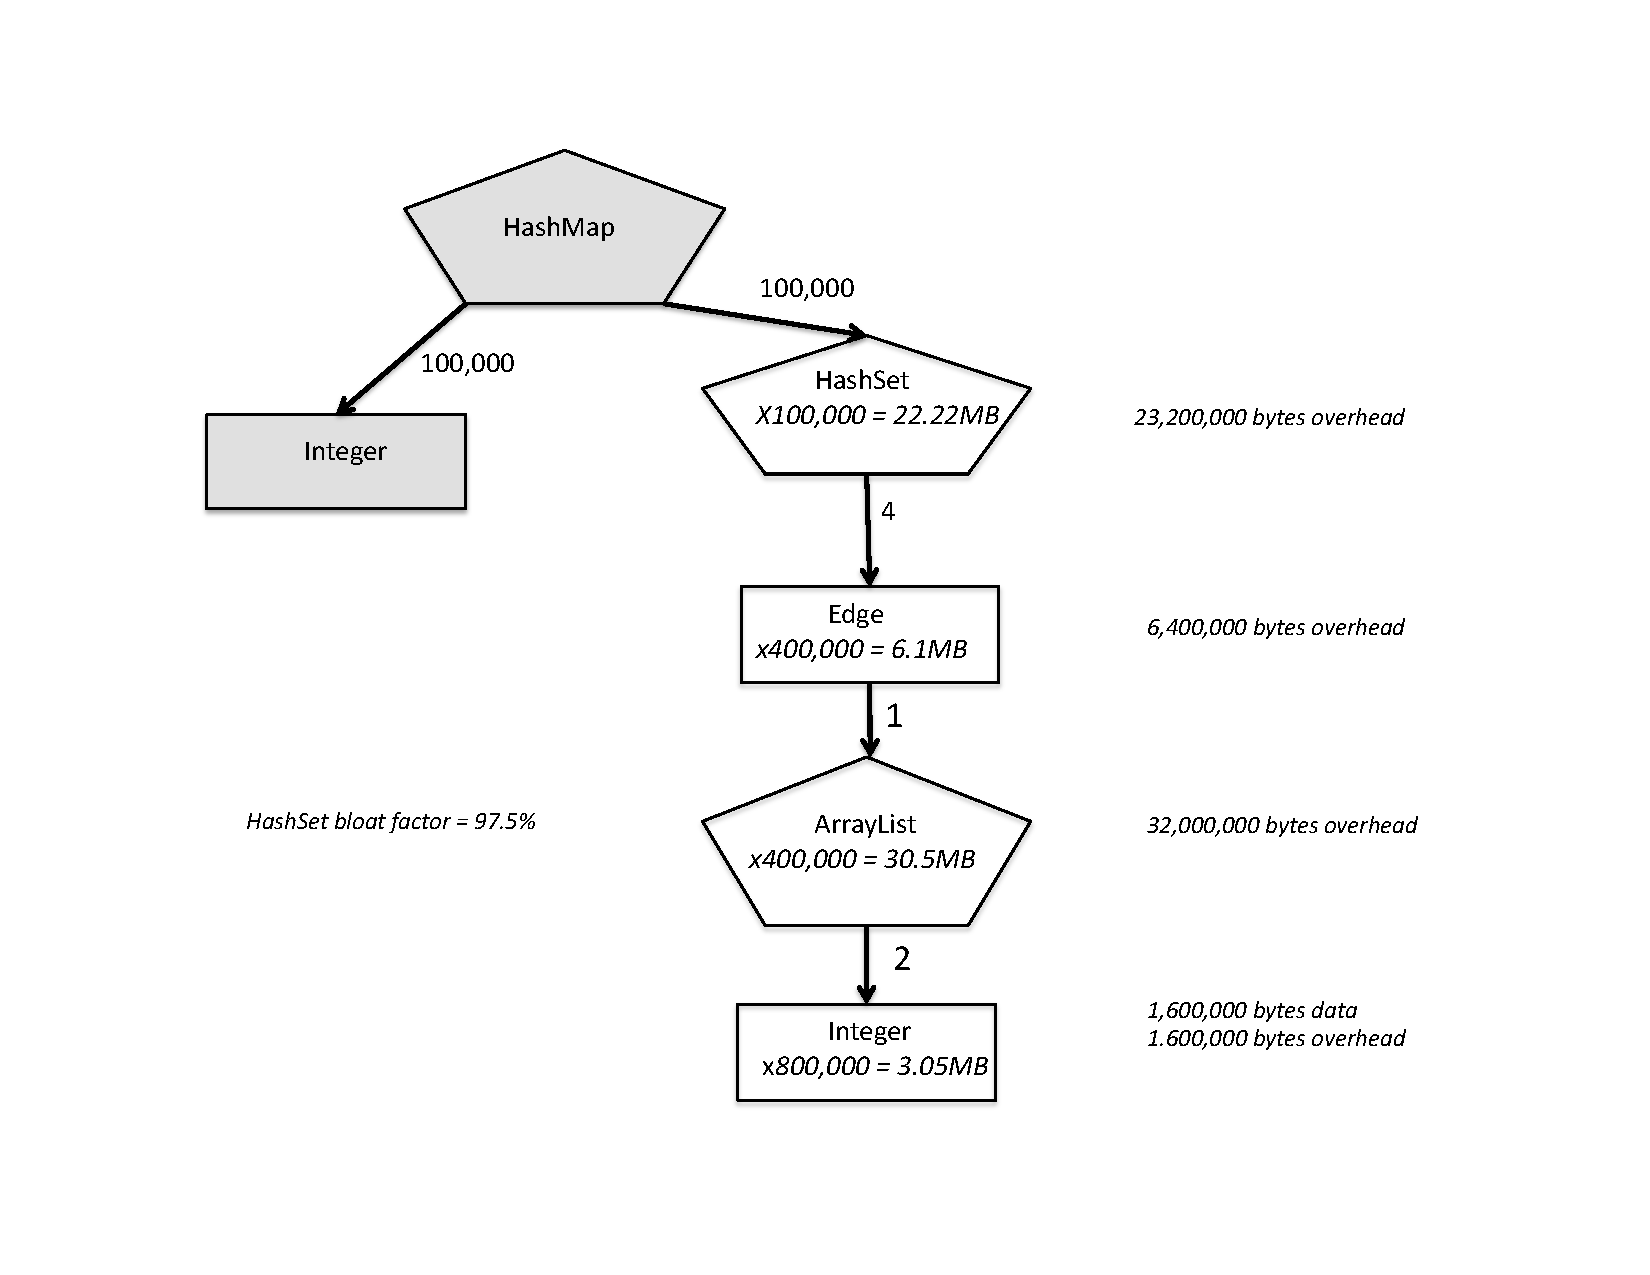
\includegraphics[width=.80\textwidth]{part3/Figures/graph-hashset.pdf}
  \caption{A 100,000 node graph, stored as a
  \class{HashMap} from \class{Nodes} to \class{HashSets} of \class{Edges}.}
  \label{fig:graph-hashset}
\end{figure}
%Sun library --  Empty HashSet -- 136 bytes
% 16 bytes HashSet (header + pointer)
% 40 byptes HashMap Object 
% 80 bytes empty array of entries

%HashMapEntry:  24 bytes:  header + 4 fields (value, key, next, hash)
% 4 entries -- 96 bytes
% total overhead for 4 entry hashset: 232 bytes
% 100,000 hashsets with 4 entries is 22.13MB

% HashMap size: 40 for header + 8 for array header
% 24 bytes per entry + 6 per entry in the array (assume extra for growth space)
% so for 100,000 entries, thats 48 + 3,000,000 bytes = 2.86MB
This example shows how easy it is to generate a lot of small collections with a very high overhead, 
in this case 100,000 four-element \class{HashSets} with a bloat factor of 89\%. Each \class{HashSet} 
by itself is 232 bytes of overhead, while four \class{Edges} have
contain only 32 bytes of data.

This implementation of a $1:n$ map is very common and
appears to be quite reasonable. However, when $n$ is small, 
the basic overhead from small \class{HashSets} 
overwhelms the data. Figure~\ref{fig:hashset} shows why a \class{HashSet} has
 such a high fixed overhead, even before any elements are added. Some of the
 overhead is Java-related, and cannot be avoided. Other overhead is the result
 of hardcoded assumptions about expected usage, that ends up being wasteful in
 the many-small-collection context.

\paragraph{Reusing HashMap} Internally, a \class{HashSet} is just a wrapper,
delegating all its work to a \class{HashMap}.
 The implementators apparently assumed that internal 
reuse is more important than keeping fixed overhead costs low, which indicates
that they didn't expect to have a lot of small hashsets, and
fixed costs are amortized for large \class{HashSets}. 
In particular in library code that is used in many contexts, specialized
implementations are often needed and reuse is sometimes a misplaced value.

In this case, the reuse has a fixed cost of 16 bytes per \class{HashSet}.
It also has a per entry cost because 
each \class{HashMap\$Entry} stores a key and a value, and \class{HashSet} only
uses the key. The value points to a constant. So \class{HashMap} is
more general than needed.
  
\paragraph{Open Chaining} \class{HashMap} itself is fairly
 expensive. The \class{HashMap} object itself is just a container, that points
 to the actual array of entries, which is necessary in Java. is using open
 chaining, which means that each hashmap entry turns into a hashmapentry object,It delegates its work to an array,
  sort of a necessity in Java, and it also has a number of bookkeeping fields,
 we will talk about in a minute.  On top of  it, 
the default size of the array, if you don�t specify something is 16. 
 So you get 16 size array, and this is all fixed cost. Before we have even
gotten to the cost of the actual entries in it. 

 similar to the treemap example last week. 
 S
 HashMap is 
expensive just for HashMap. It could be much more specialized for HashSet. 
And we also have the default size of the array. The third problem is that hashmap 
has a bunch of bookkeeping fields in it, that really are rarely needed, 
and certainly not needed all together. It has a bunch of fields to keep different 
views of the hashmap that you might want. The map interface says that you can 
compute a collection of all the entries, all the keys, and all the values.
 And HashMAp caches all of those. So every HashMap, and every HashSet, is paying these three 
 pointer costs, which is an extra 12 bytes. In fact, you rarely use all three together, and 
 it�s not all that common to use even one of them. 

The other thing is that the hashmap entry itself is storing a hashcode. 
It�s maintaining a hashcode, even though the most common cases are keys, 
either strings, store their own hashcode. Or integers, where the hashcode 
computation is pretty trivial. So that�s also a misplaced optimization, 
and you have to ask the question. Was this based on an empirical study, 
with possibly the wrong benchmarks, or was this based on some assumptions? 
In this case, it was sort of another cautionary tale for library designers of 
the danger of premature optimizations.

O the end result is that HashSet is a pretty poor choice if you have small sets. 
 At least with its current implementation. Obviously, it�s worth measuring here. 
 And indeed the developer did, and was able to solve the problem. Some other 
 lessons in here about what the developers of hashset must have been thinking, 
 and really for anyone who is developing a library of framework that is going to 
 be used higher up. Basically, they hardcoded in a lot of the assumptions about 
 its expected usage.
 

\section{Transforming Fixed Size Collections}

Getting back to our example, the developer looked and said, I actually 
don�t need the hashset functionality, because the only difference in functionality 
between a hashset and an array list is that the hashset was guaranteeing 
uniqueness, and it turns out the developer was already guaranteeing uniqueness 
in the loading code, so this was just put in as an extra failsafe thing, just in 
case there was a bug in the higher level code. When the developer saw this, 
he said, that extra check is not worth the cost. Was able to replace this with an 
arraylist, and for this piece of the structure was able to get 77\% savings
pretty easily.  Obviously, if we could have collections that worried about all 
of this stuff for you. A set that grows more gracefully, that you didn�t have to 
pay a high fixed cost for a tiny little set, then it would be very nice.

L
\section{Properly Sizing Collections}

 Let�s talk a little bit about default sizes and growth policies, and that 
 sort of thing. So this is a little hypothetical experiment here. We�re getting 
 back to the value side of this structure, where you replace the original 
 hashsets by arraylist. He sized them minimally, but having not done that, 
 had he taken the default sizes for the arraylists, it would have cost another
 28\% of overhead, since all the collections, basically are sized pretty 
 aggressively just like StringBuffer is, with this idea of trying to reduce 
 the copying costs and basically assuming that any collections you have are 
 going to grow, and so we�d better pay those costs up front in large chunks, 
 so that you don�t have to constantly pay a reallocation, and copy costs, 
 and it�s really an open question of whether that�s buying us any performance 
 or not, it�s certainly costing people a lot of footprint. One of the common 
 patterns we see is people just take the default size of collections. 
 They just take the constructor, no parameters, and even when they do 
 specify a default size, the collection growth policies are still pretty 
 aggressive. Typically double in size, and there�s even one copy constructor 
 that one of the array list copy constructure, if you hand it a collection and 
 say make me an arraylist out of this, it actually adds 10\% to it, just in
 case you grow this thing. And the typical pattern is you are building some 
 temporary collection to sort something or filter something, and at the last 
 minute you are done with it, and you turn it into an arraylist that you are 
 going to send onto somebody else, and they are not going to modify it again. 
 So there is definitely optimization for some questionable cases in here.

What can you do about this? One is that you can set the initial capacity 
relatively low. If you might be introducing a performance problem then do 
some timing, and see if it�s actually the case. Another thing is if you have 
data modes and many data models have this pattern, where you have a load phase 
vs a usage phase. I load all my data, and I never modify it again. Or maybe 
I�m modifying entries but never adding anything , then you can use  trimToSize. 
Just walk through the whole data model and call trimToSize on every collection. 
You will pay a reallocation and copying cost just once, and that�s it. 


Just a quick look at some of the default sizes. LinkedList, 
it�s not really applicable other than the fact � always comes with an 
extra entry as a sentinel, just to make the coding of LinkedList simpler, 
So you are actually paying 3 entry cost for a 2 element collection. 
ArrayLists, the default size is 10. For some reason, the latest J9, 
in these Harmony classes, which are open source, they�ve upped it to 12, 
and I�m not quite sure why they�ve done that. Actually that�s not really true.
 The default size initially for an empty collection is 0, so they�re still
 allocating the array with 0 size. Where as the Sun and older JVM�s are always 
 allocating 10 element collection. But on the Harmony classes, the new J9, 
 after you add the first element, they jump it to 12. It�s pretty hard not to 
 get those big jumps in these collection classes. HashMap, the default is 16, 
 and HashSet as well, since it�s based on HashMap. So it�s definitely 
 worth setting the default in these cases where you know you have mostly these 
 small collections. 

\section{Avoiding Empty Collections}

A related problem is empty collections, and this is super, super common. 
People are eagerly initializing things, and without realizing that the empty 
collections are pretty costly too. This was the case from JPMorgan 
Chase critsit, that Nick did, and in fact in SessionState, which had all sorts 
of other stuff in it, had these profile objects in it, which were profiles of 
customers, and each of those profiles was a highly delegated design, we saw it 
last week, each one had 40 instances hidden inside that box. 

For those of you who weren�t here last week, this notation is kind of a UML-like 
notation This is a logical data structure and these boxes are hiding other classes.
 The octagonal shaped ones are collections, things implementing relationships. 
 SO profile had quite a few classes inside it, and they all had the same coding 
 pattern in them, where they had these arraylists hanging off of them. 
 In one case it was to track the history of modifications in various fields. 
 In total, each usersession data had 210 empty arraylists hanging off of it, 
 which was rather expensive in this little example here. They were paying  
 8MB in this of just empty arraylists. So what are the remedies here? 
 The simplest thing is to lazily allocate these things. Along with lazy 
 allocation, there�s a nice static method in the collections class, 
called emptyset, where it will return you a pointer to a singleton empty set 
that has all the functionality of a set. EmptySet, EmptyList, EmptyMap, and 
those are great since you can point to them, and the size method will still work,
iterators will still work, all that stuff will still work, and you don�t have 
to allocate an empty collection. The only bad thing with those 2 patterns, 
and you really have to watch out for, is if you give out any references to your 
collections before they�ve been allocated. Because once you give out a 
reference, you expect people to hold on to it, then there�s no way to morph it 
into this other form that�s actually populated. And that�s a serious issue in Java.
 But if you can hide the references within the class, then this is very easy 
 to fix. 

So just a quick look inside the empty collections, you can see that they are not 
all that empty. So all the standard Java collections eagerly allocate their 
subsidiary objects, which means that every empty collection consists of 2 objects, 
2 object headers, a pointer, plus whatever bookkeeping fields they have. 
So you get these rippling effects, you have a really high level code, that�s 
eagerly initializing some package, and it�s eagerly initializing some thing else,
 and eventually it�s initializing some collection, and the collection is doing 
 the same thing; it says, well I�m just going ahead and allocate my array, 
it�s not clear why, it�s either ease of coding, or to avoid an if statement 
check at runtime, it�s not clear. So another area is to see if there�s any 
 performance benefit to this, or is this something that can be changed very 
easily. And juust a quick look at the cost of the empty collections. 
What strikes me � these are the number from both sun and IBM. What strikes
me is that the smallest number here is 48, so there�s certainly no single 
digit anything in Java, but 48 is a pretty high number for something that�s 
empty, if you are going to have a lot of them, and also, there�s a little bit 
of variation, both having to do with whether you�ve made the size default or not, 
and also what kinds of collection class you are choosing.


\chapter{Scalability}

So that was all about small collections, and their problems. We kind of segwayed into the other half of the collection problem, which are collections that have high per entry costs. Typically large collections, but not always. Our design 3 really suffered from that. Basically, it has a high constant cost per entry. Just like our tree map did last week in the  health example. So each of these, just the per vertex and level cost here, is 48 bytes. It�s 28 bytes per enty in this hahsmap, and 20 for the pair objects.  It�s a constant cost that won�t be amortized. This is a theme that shows up in a lot of Java collections, in particular larger ones. Just a quick look at the per entry costs.
They are fairly high other than for arraylists. HashMap and HashSet is 28 or  36. ArrayList is the lowest I�ve seen. and LinkedList is 24 for again, this is purely because there is a separate object in the collection, delegating to your object. And that doesn�t include the cost of any boxing you have to do on your side to introduce a pair class, or a cap int, or anything like that.  That could easily double some of these numbers.

So it�s pretty common to see that in large collections, like in example we just saw. Another case is when you have nested small to medium sized collections, that still have enough entries to have high per entry costs. And this was the case in the SIP container that ws being used in the SAametime Presence server. This also had a requirement of maintaining a large number of subscriptions active at the same time. So this is handling stuff like when you�re sametime window is open, telling you who�s on line, what everyone�s status is. So this has to keep some huge number of statuses sessions active for various people. And so what they did here is the presence server employed the sip container to use a feature in websphere to store information in sessionstate about each of these subscriptions. So there�s quite a few layers in between, and basically they had 7 properties of each subscription they used to store. Basically, each of the 7 properties had a name, a string, and some kind of value, and most of the values were scalars. There some cases where they weren�t, but just for simplicity here. They just called the websphere, and websphere, said to add this to the sessionstate for each of these properties. And websphere stores the session state in some framework it has, as a hashtable of attributes and values. So it just stores each string with the values. Now fortunately, they did something really good here.   All of the subscriptions were storing the same 7 attributes so all the attributes were the same. At a higher level, presence server was sharing the strings. So at least they didn�t� have 20,000 copies of the same seven property names, when they had 20,000 subscriptions. But what was costing the so much here the hashtable per entry costs, and the cost of boxing up all of these scalars, because that�s what websphere interface requires to store all these things. It was attribute, and cap object property. So this was something that was obscured by all the layers between. The decision is it�s very hard to say webshpere, fix this code for us, because that code is being used by all kinds of people, all over the place. So fortunately they came up with a pretty reasonable solution, which was that the presence server packaged all 7 of their properties into a single object, and then stored that subscription property object as a megaproperty, and that cut the per entry cost by 7. So that is an interesting hybrid example. Still relatively small collections, but it was really the per entry costs that were getting them. We�ve seen this a number of times.

So now just some special purpose cases of thes high per entry costs. That example from last week, Treemap of mapping doubles to doubles, and this was the real-world case that it came from. this is actually 1.2 or 1.4G structure. There were 52 treemaps, and in total there were 13 million entries in them. And the per entry costs was what 88 bytes per entry, again, same reasons. The alternative is to just use a collection that is optimized for scalars. This is super, super common. In fact there was a document processing application that where pretty similar kind of thing mapping Integers to Integers. In general collections of scalars suffer from these kinds of problems. And the solution is to have a specialized collection, outside the java collection for scalars. One of the issues is to standardize them somehow.

Another specialized collection is what�s called the Identity Map.  It�s for the case where your key is an object reference, and you know that�s going to be stable. In some sense this breaks your map interface standard, because Identityhashmap is a standard Java library cache, uses == rather than .equals to do its lookup. The common case is if I�m maintaining a proxy object for some other object, so I can make the proxy the key, and the vaue is the real object behind it. There�s always the pointer to the proxy that you want to use as the key. If this is stable, and your not counting on the value of it, then this is a great implementation. Just a little experiment I did, I tried implementing it as a standard HashMap, I put 10,000 entries into it, and then I use the Identty hashMap, and there was a pretty huge reduction, 59%, this was with the SUN JVM, IBM JVM was almost as good as SUN in this case. The main reason this was more efficient, I think isn�t just because of the ==, the main reason I sthey are using open addressing, rather than open chaining. They are not creating a different object for each entry. They actually have parallel arrays. In this case they have 1 array because they don�t need to store a key. They have one array that has the keys and values in it interspersed, if I remember. So this is a good class to know about, if you have a use case.

Just a summary of colllecitons.
There are really 2 classes of scaling issues. One is you have small nested collections, and you are paying the fixed cost of small collections, plus you may be paying per entry costs, if they have high per entry costs too for the small collections. The other case is the per-element costs of larger collections or nested collections, and any data delegation costs that those occur of the objects you store in them.

Just a little more about standard collections. The focus has been speed. Or supposedly it has been speed. It certainly hasn�t been footprint. There�s been very little attention given to that. I was a little surprised to see in the harmony classes. They harmony classes are the newest classes for J9, version 6. They have been open sourced on Apache. I was surprised that Harmony, I thought this was great, they finally fixed some of this stuff, and I found that they actually increased the footprint in a couple of cases. They added an extra field to arraylist, they made some of the sizes bigger. They cut the footprint in a number of cases too, but nothing substantial. I think the more disturbing part here, is the fact that a lot of the assumptions are hard wired. So there are not a lot of policy knobs to play with when you are coding to these things, and that�s really a problem. 

And finally, some of these specialized collections are worthwhile for their functionality, if not only for it�s footprint. The identity map is worthwhile for its footprint. Just some alternative collections. Like I said, the Apache commons collections are really nice from a functional perspective. They are not really doing much for footprint from what we can tell, at least from the code I�ve looked at. The Trove collections are great for footprint, but we are not allowed to use them, at least from what I understand. Anything you work on that may go out, you really have to check specifically.   The opensource licensing stuff, it�s on a product by product basis. There�s a lot of collection class efforts Amino classes are aimed at concurrency, Javalution from Raytheon is for soft realtime, and externally on sourceforge, Cliff Click has some non-blocking collections. Actually, he claimed the footprint is good. I haven�t seen any studies on it. The best source of good collections I�ve seen are actually scattered around the IBM frameworks. Portal, Rational, just all over the company.

Developers have a tough situation. Choosing the collections not always obvious what the choices are. Purpose, to raise the awareness. What kinds of things to think about, what to measure. Not to think that things are cheap. And in this context of expensive implementations, sometimes you do hit walls, and there�s nothing you can do. But sometimes you really can fix a number of problems. There�s a lot of problems that have easy solutions. Choosing the default size, lazily allocating collections that are most likely to be empty. Picking a collection with less functionality if you don�t need the full functionality. I strongly advise not writing your own collections, unless you really have search the company for something that will do the job, because it just introduces a whole other set of problems.

Implementing a cache, relationships, a nested map, attribute-value pairs etc � global optimizations. Study � what�s most of the heap?  Which kinds of database bulk storage optimizations would be appropriate?


Chapter: SPECIAL COLLECTIONS


Multikey

I said this was a pretty common programming idiom, and in fact I was looking around the Apache commons collections, which is a fairly nice, open source set of collections, they have something called a multikey map. Great, maybe they are solving this already. They have, like every other collection, they have a wrapper object, and then they have an array, and inside that it�s an array of these multi-key objects, and I thought this is nice, you�ll subclass this thing, and then you�ll be done. Instead what they do is that in turn delegates to another array, which has the different parts of the key in it, and your keys get added to that. So in fact, this is even more expensive, maybe it�s about the same, because it has a wrapper multikey which is equivalent to an arraylist object, and then the array is just like the array that was inside the array list. So the could have easily implemented something. There are calls in this class, there�s a put call with 2 keys, and a put call with 3 keys, and a put call with 4 keys, so they could have easily have specialized this, and had a multikey 2, and a multikey3, and so forth that were subclasses of multikey, that had the right number of fields in it. But, it was just the focus here. SO that�s another 20bytes per entry in this case also. Frankly, as I looked around at a lot of the standard collections out there, there�s just no attention to footprint. 

CONCURRENT MAPS

So now some special cases in this. There are a lot of different uses of this, and one interesting things we�ve been learning, as we�ve been looking at all these case studies is that we�re really trying to think about why are people using collections, and what are they using them for? In the last example, we saw, they are using them to implement a map. A fairly complicated map. In that first long example. 

This example was from one fo the SameTime products, Lotus server-side products. I have a lot of Lotus examples here, only because we�ve worked with the a lot. Not because their code is worse than anyone elses. This is a pervasive problem. 

So in this case, this is the sametime gateway actually, and what it�s doing is keeping track of active chat sessions. Example is a bit simplified. They need to handle some gigantic number of concurrent sessions. So they use a concurrent hashmap, the standard Java concurrent hashmap, and in that they store sessions. Each session has some number of subscribers, and so within each session they use a concurrent hashmap to store the subscribers. When we look at this together, everyone was in shock that this concurrent hashmap thing was so huge. And again this was a relatively small run, but even for this, we didn�t expect there to be 177MB of concurrent hashmap. And so we looked at it, and it turns out they took all the defaults for concurrent hashmap, and each concurrent hashmap costs 1700 bytes, approximately. The reason for that is that the concurrent  hashmap is really designed for high concurrency, so it contains 16 parallel hashmaps by default, each with 16 elements. Now if you only have a few subscribers, most of that stuff is empty. So when the developers saw this, they immediately realized, we don�t need that kind of concurrency control. We don�t have thousands of subscribers on the same session. We need that concurrency on a higher level. Sure, we need a concurrent hashmap up here to manage hundreds of thousands of sessions, but each session is only going to have a few subscribers. So we can greatly limit the number of concurrency we can support there, as long as it�s thread safe. So one developer suggested, ok , let�s just take the concurrent hashmap, and choose the default as 3 instead of 16. With that, they could have gotten a reduction of 67%, which is substantial, but then one of the other developers suggested let�s just use HashTable, because it�s much, much smaller, and it�s still threadsafe. So hashtable was a great choice for the sametime people, as it turned out.

UNMODIFIED MAP

So here� another example, of unmodifiable, now this was from NetFlix, which Nick analyzed, it was an IBM customer, and in this case, we don�t know exactly what this was, some kind of cache of titles they maintained, and it had also a 2-level structure to it, and it had in this particular run 2 million of these inner maps, taking up about .5G, and when we looked inside there, what we found, was that each of those maps was an unmodifiable map, wrapping a smaller hashmap, so they had 2 problems. One was why they had the small hashmaps, and that�s a separate issue, but even the unmodifiable hashmap was pretty substantial. This was a 64 bit JVM, I think this was a SUN JVM, so the cost was even double of what we say before, it was 56 bytes for each of these wrappers. It was a pretty hefty cost. So this is the kind of thing where � this is a functionality that. Unmodifiable is pretty useful for development time, to avoid programming errors, but it�s not clear that especifallly, this fine grain, that in deployment you would want to keep a feature like that in there, this is pretty expensive.  

There�s a whole set of Java wrapped collections, for type checking, for modifiable, and that�s the general pattern. That�s a nice programming pattern, and it certainly simplified the class hierarchy. I read some of the notes from the designers of these collection classes, about why they made these choices, and they said it would just have complicated the class hierarchy in the Java collection classes to have all these combinations there. And that makes perfect sense when you have a few large collections. But in this kind of case, when you have lots and lots of small collections, it really adds up. On this JVM, this is 1.4.2, maybe this we sun 1.5 the cost is 28 bytes per each of these wrapper objects, which is pretty substantial. So that�s including its header, its bookkeeping, and the pointers. That�s ok for large collections, for small collections, it really adds up. 



\chapter{Specialized Collections}

\part{Managing Object Lifetime}

\chapter{Lifetime Requirements}
\index{Lifetime Requirements}

Your application needs some objects to live forever and it needs the rest to die
a timely death. Unfortunately, some of the important details governing memory
management are left in your hands. Java promised, with its automatic memory
management, that you could create objects without regard for the messy details of
storage allocation and reclamation. In Java, you needn't explicitly free objects,
which is at once the saviour from, and the source of, many problems with memory
consumption. Unless you are careful, your program will suffer from bugs such as
memory leaks\index{Memory Leaks} or excessive peak footprint. Furthermore, if
your objects don't easily fit into the limits of a single Java process, you will
need to manage, explicitly, marshalling them in and out of the Java
heap.\index{Marshalling}

Very often, your application uses a data structure in a way that falls into one
of a handful of common \emph{lifetime patterns}\index{Lifetime Patterns}. The
nature of each pattern dictates how much help you will get from the Java runtime
in the desired preservation and reclamaion of objects, and where it leaves you to
your own devices. \emph{A necessary step in the design process of any large
application is understanding into which lifetime pattern each of your data models
fit}. The five common lifetime patterns are: objects needed only transiently,
objects needed for the duration of the run, objects whose lifetime ends along
with a method invocation, objects whose lifetime is tied to some other object,
and, most difficult of all, objects that live or die based on need.
\autoref{tab:five-lifetimes} summarizes these five important patterns. We step
you through each of the patterns, defining them and giving examples of how to
know when you have an instance of each. In the next chapter, we show how to
implement these patterns.

%The trickier aspects of memory management, summarized in
%\autoref{tab:tricky-memory-management}, are discussed in greater detail in
%later chapters.

\begin{table}
\centering
	\begin{tabular}{lp{0.30\textwidth}p{0.35\textwidth}}
	\toprule  & Lifetime Property & Example \\ \cmidrule(r){2-2} \cmidrule(l){3-3}
	\autoref{temporary-lifetime}  & {Temporary} & new
	parser for every date
	\\
	\autoref{forever-lifetime} & {Needed Forever} & product catalog
	\\
	\autoref{correlated-lifetime-1} & {Correlated with Object}
	& object annotations
	\\
	\autoref{correlated-lifetime-2} & {Correlated with Phase} &
	DOM used only for parsing
	\\
	\autoref{deferred-deletion} & {Correlated with Need} &
	pooled Strings \\
%period\\ scoped to a phase/request\\
%correlated with an object (annotations)\\
%correlated with need}\\ \hline
%reusable & maybe i'll need it later \\ \hline
	\bottomrule
	\end{tabular}
	\caption{Five important categories of object lifetime.}
	\label{tab:five-lifetimes}
\end{table}

\section{Examples from a Server Application}

Configuring memory settings is an iterative process. It usually involves a
fair amount of trial and error, as one tunes the various knobs to balance memory
consumption and application performance. These knobs affect things like the size of the Java
heap, how many entries a cache should hold, and the timeout value for these
caches. This is usually a process of black box tuning: twist a knob, and see
how overall performance changes. In addition to being hit
and miss, it is also quite prone to bugs. If you set the size of a cache too
high, you risk poor performance due to excessive garbage collection, and even
possibly process failures, due to running out of heap space.

Tuning memory consumption in long-running applications, such as servers or
integrated development environments, is a particularly thorny issue. Improperly
managing memory in a short-running application may not be the end of the world.
In an application that runs more or less forever, mistakes can pile up over time.
In addition, they synthesize information from a diverse array of sources, each
with its own performance trade-offs. As such, caching plays a large role in these
applications. Consider an example from a server aplication.

\begin{example}{Object Lifetimes in a Server Application}
A web application commerce server preloads catalog data into memory to allow for
quick access to this commonly used data. It also maintains data for users as they
interact with the system, browsing and buying products. Finally, it 
caches the response data that comes from a remote service provider that charges
per request. How does Java heap consumption vary over time? Which heap size
fluctuations indicate a problem, and which are expected behavior?
\end{example}

\begin{figure}
	\centering
	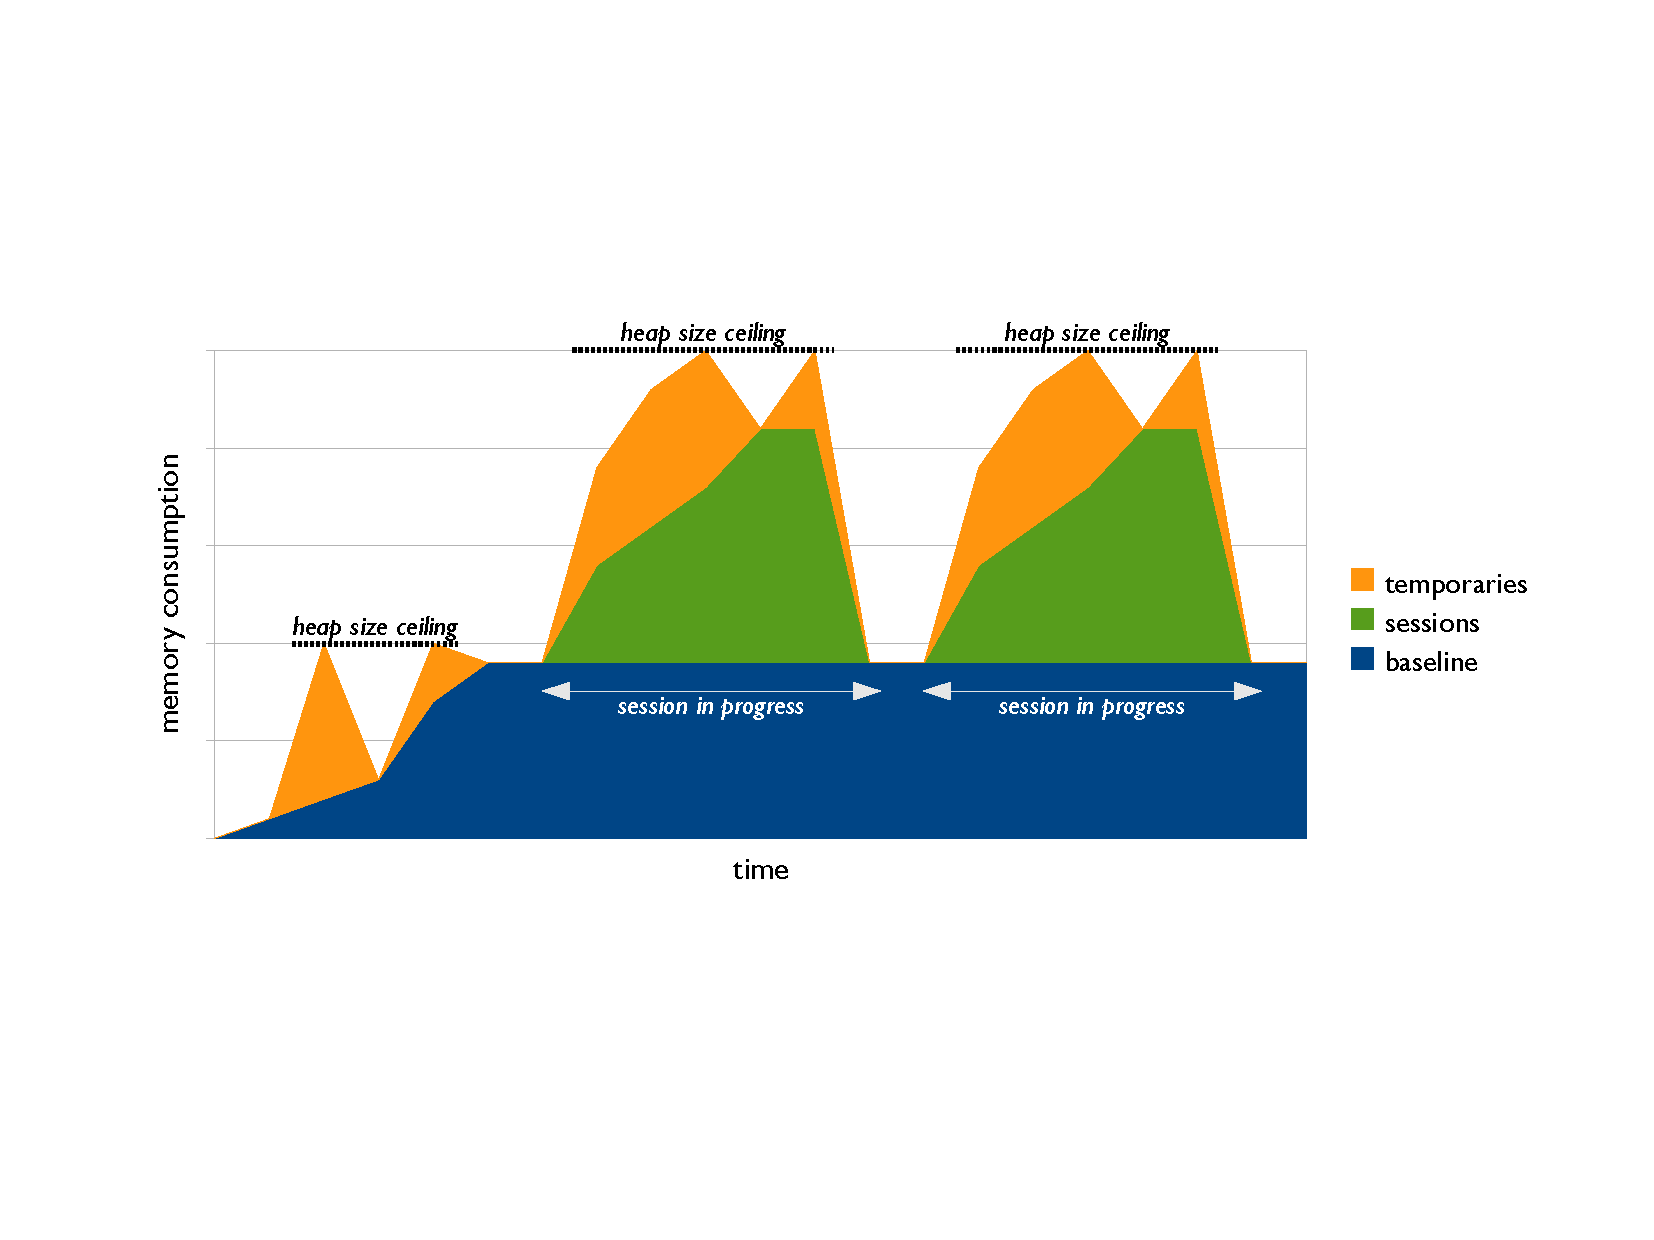
\includegraphics[width=\textwidth]{part4/Figures/lifetime/timeline-base-session-temps}
	\caption{Memory consumption, over time, typical of a web application server.}
	\label{fig:timeline-base-session-temps}
\end{figure}

The heap consumption of this application will fluctuate over time. A timeline
view expected memory consumption helps to illustrate the five main kinds of
object lifetime. It visualizes memory during the lulls and peaks of activity, as
requests are processed and when sessions time out, and as the server starts up.
 \autoref{fig:timeline-base-session-temps} shows an example timeline
for a server that, as it starts up begins to load catalog data into the Java heap.
Then, it responds to one request at a time. The total height of the area under
the curves represents the memory consumption at that point in time. 
In this example, as the server starts up, it begins to load catalog data into
the heap. This data will be used for the entire duration of the server process.
\index{Objects That Live Forever}
The Java objects that represent this catalog are objects that are needed
forever. In the timeline picture, this data is respresented by the lowest area,
labeled \emph{baseline}. Notice how it ramps up quickly, and then, after the
server has reached a ``warmed up'' state, memory consumption of this baseline
data evens out on a plateau for the remainder of the run.

\index{Session State}
After the server is warmed up, it begins to process client requests. Imagine
interacting with a commerce site. First you browse around for items of
interest. You may add items to your shopping cart. Eventually, you may
authenticate and complete a purchase. 
As you browse and buy, the server may be maintaining some
state, to remember aspects of what you have done so far. This
session state, at least the part of it stored in the Java heap, will go away
soon after your browsing session is complete. In the timeline figure, this
portion of memory is labeled \emph{sessions}. It ramps up while a session is in
progress, and then, in the example illustrated here, soon all of that session
memory should be reclaimed.

The catalog (baseline) data and session state are both examples of objects that
are expected to stick around for a while.
\index{Temporary Objects}
 In the course of preloading the cache
and responding to client requests, the server application will create a number
of objects that are only used for a very short period of time. They help to
faciliate the main operations of the server.
These temporary objects will be reclaimed by the \jres garbage collector in
relatively short order. The point at which an object is reclaimed depends on when the garbage collector
notices that it is reclaimable. Normally, the garbage collector will wait until
the heap is full, and then inspect the heap for the objects that are still
possibly in use. In this way, the area under the \emph{temporaries} curve has a
see-saw shape. As the temporaries pile up, waiting for the next garbage
collection, they contribute more and more to memory footprint. Normally, once
the \jre runs a garbage collection, these temporaries no longer in use will no
longer contribute to heap consumption.

In this way, temporary objects
\emph{fill up the headroom} in the heap.\index{Heap Headroom}. If there is a
large amount of heap space unused by the longer-lived objects, then the
temporaries can be reclaimed less often. This is a good thing, because a
garbage collection is an expensive proposition.
\index{Heap Size Settings} \index{Maximum Heap Size} \index{-Xmx}
When configuring your application, you may specify a maximum heap size. It
should certainly be larger than the baseline and session data. How much
larger than that? This choice directly affects the amount of \emph{headroom},
 that is the amount of space available for temporaries to pile up.

\begin{figure}
	\centering
	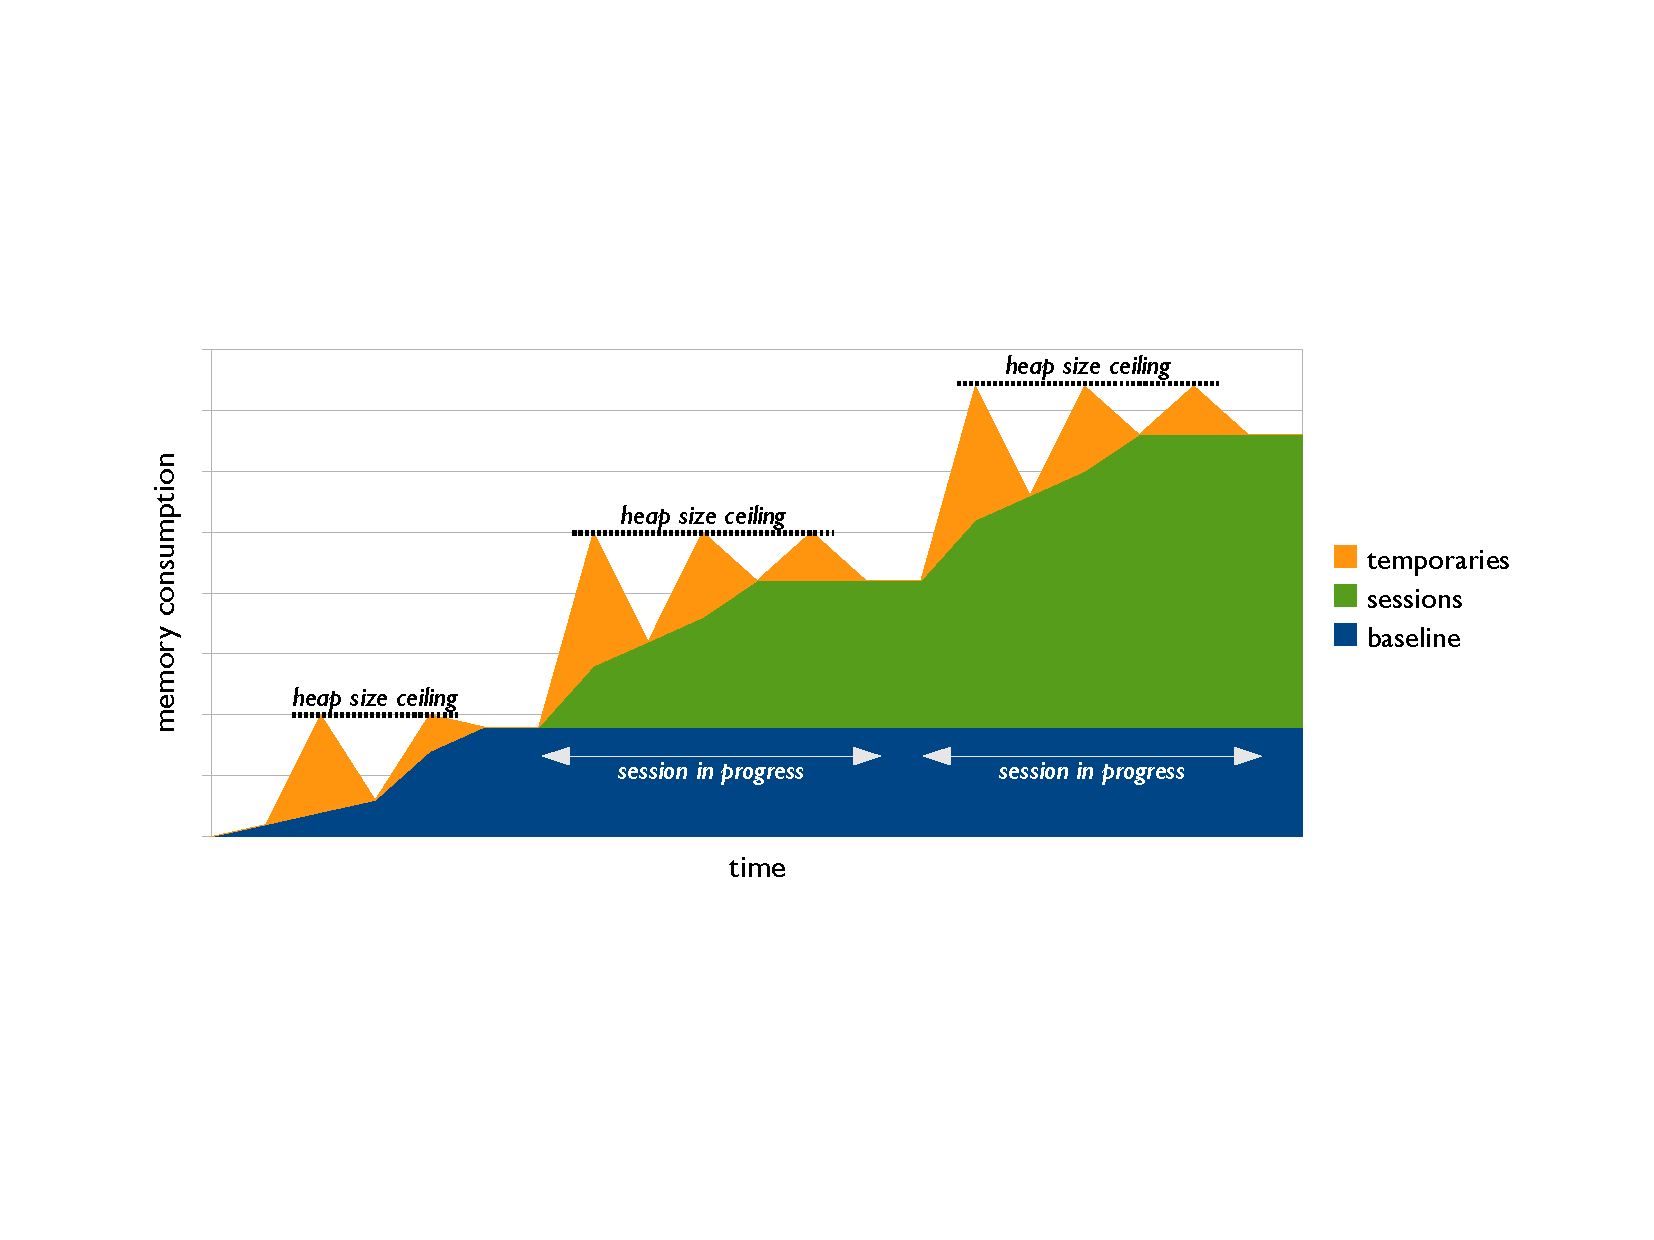
\includegraphics[width=\textwidth]{part4/Figures/lifetime/timeline-base-session-temps-with-leak}
	\caption{If session state is not cleaned up
	properly, a memory leak is the result. This means more frequent garbage
	collections, and ever increasing heap size.}
	\label{fig:timeline-base-session-temps-with-leak}
\end{figure}

\index{Memory Leaks}
The catalog data should last forever, while the
session data lives for some bounded period of time. It is possible that session
state will live beyond the end of your session, but nonetheless it has a
lifetime that is bounded. If, due to an bug, part of this session state is not
reclaimed, the application will leak memory. Though it is supposed to have a bounded lifetime, it
\marginpar{\textbf{Memory Leaks} are still possible, even with
automatic garbage collection!} accidentally lives forever. In this
case, over time, the amount of heap required for the application to run will increase without bound.
\autoref{fig:timeline-base-session-temps-with-leak} illustrates this situation,
in the extreme case when all of session state leaks. Over time, the area under
the curve steps higher and higher.

%As you scan the timeline from left to right, memory consumption 
%it fetches catalog data from its database, and stores them in the Java heap. 

Finally, this example server caches data from some expensive third-party data
source. When caching data inside of Java objects, there is a fourth effect on
the timeline landscape. The
cached data must be configured properly to live long enough to be useful. It
also must not occupy so much of the heap so as to leave little headroom for
temporaries. \autoref{fig:timeline-base-session-temps-with-cache} shows an
example where the cache has probably been configured to occupy too much heap
space. Observe how, compared to the other timeline figures, there is little
headroom for temporaries. In this case, the result is more frequent garbage
collections. If the cache were sized to occupy an even greater amount of heap
space, it is possible that there would no longer be room to fit session data.
The result in this case would be failures in client requests. So, as you can
see, sizing caches is important. As discussed later, it is very tricky to
properly size caches, and is something best left in the hands of the \jre.

\begin{figure}
	\centering
	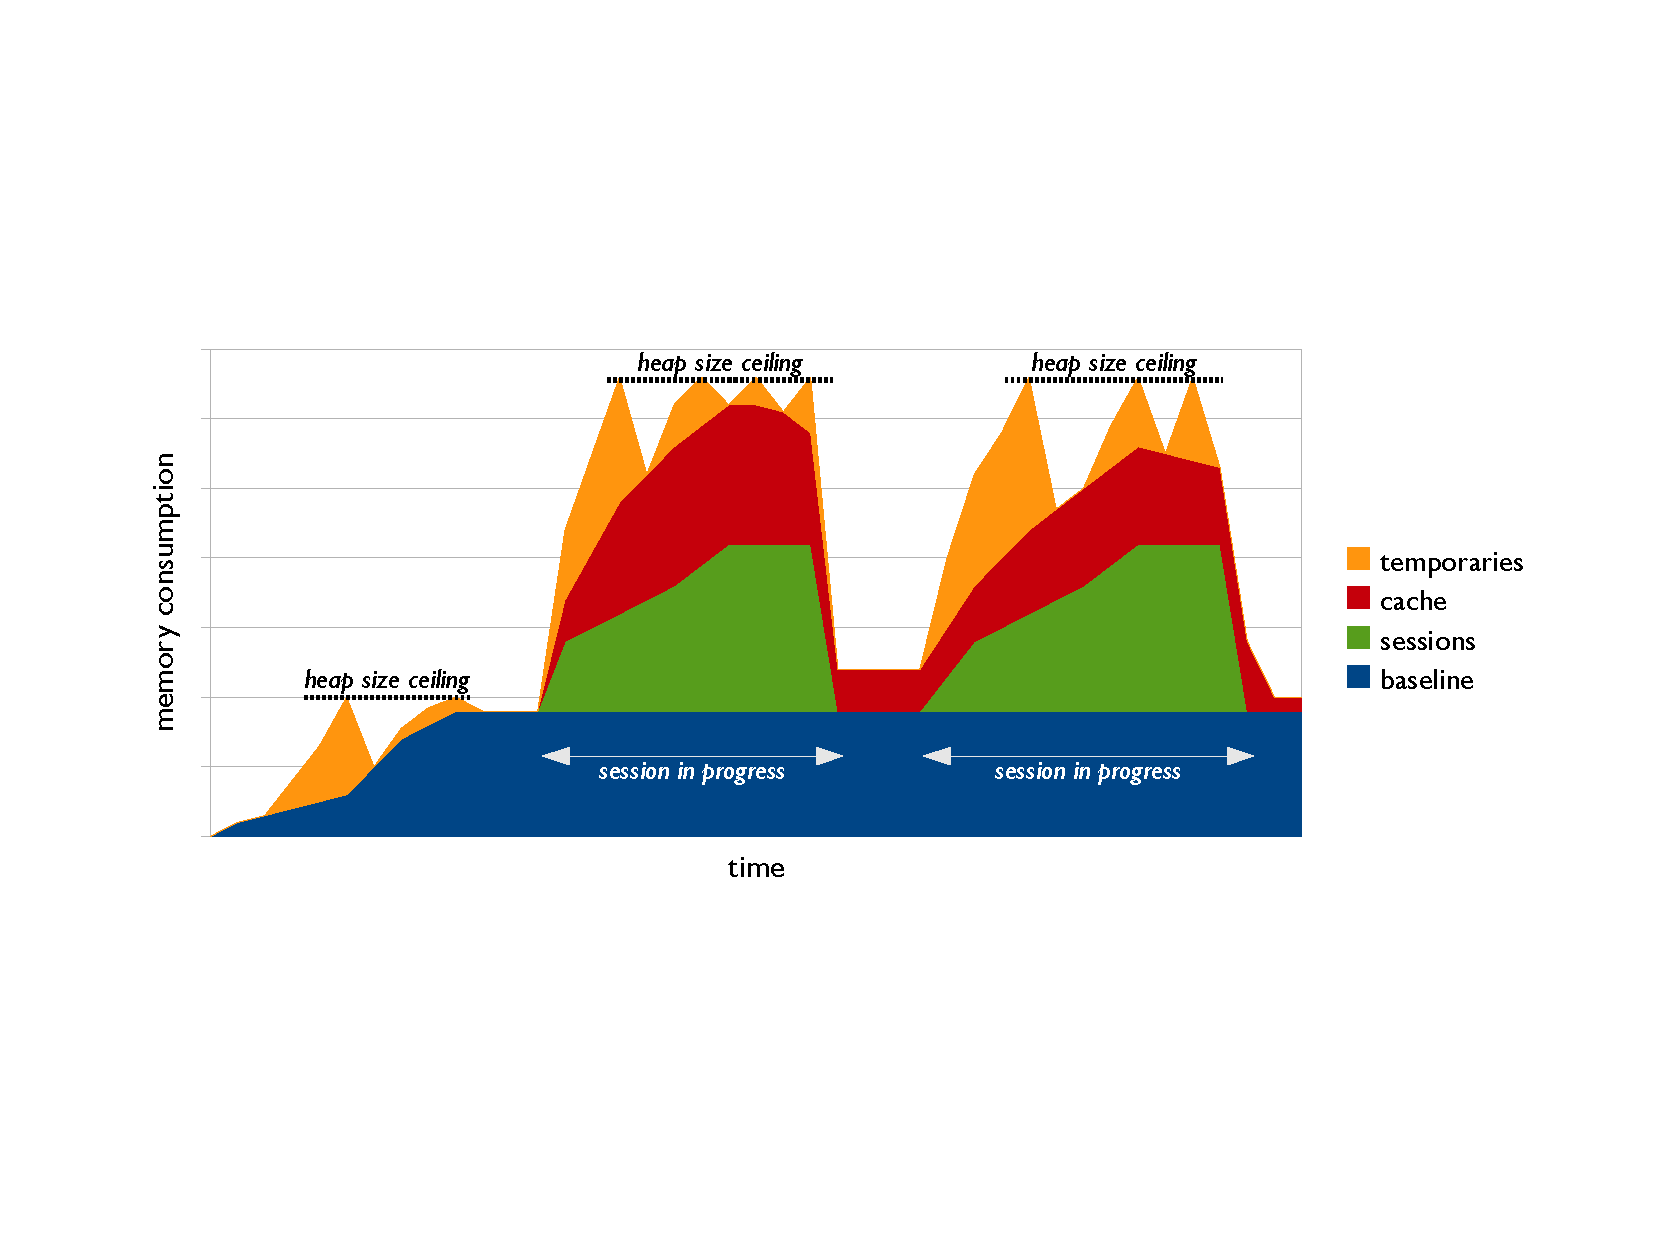
\includegraphics[width=\textwidth]{part4/Figures/lifetime/timeline-base-session-temps-with-cache}
	\caption{When a cache is in use, this leaves less headroom for temporary
	object allocation, often resulting in more frequent garbage collections.}
	\label{fig:timeline-base-session-temps-with-cache}
\end{figure}

% introduced by example in this chapter, and
%Many objects are either temporaries or needed for
%the entire run of your application. Sometimes you create objects whose lifetime
%is correlated with other objects or that should go away when a method
%invocation completes. Sometimes you need to manage objects hanging around
%longer than their current need, to avoid future recomputations or refetching
%of data in the case when it is needed in the near future. 

%\begin{table}
%\centering
	%\begin{tabular}{ll} \toprule
    %%%%	%& Things Java Doesn't Do Automatically \\ \cmidrule{2-2}
%    	\autoref{avoiding-lifetime-bugs} & {Avoiding Memory Leaks} \\
%    	\autoref{balance-time-and-space} & {Balancing Time and Space} \\
%    	\autoref{outisde-java-box} & {Supporting Massive Data Sets}  	\\
%        \bottomrule
%    \end{tabular}
%	\caption{The tricky aspects of memory management.}
%	\label{tab:tricky-memory-management}
%\end{table}

\section{Temporary Objects}
\label{temporary-lifetime}

If your application is like most Java applications, it creates a large number of
temporary objects. They hold data that will only be used for a very short
interval of time. It is often the case that the objects in these transient data
structures are only ever referenced by local variables. For example, this is the
case when you populate a \class{StringBuffer}, turn it into a \class{String}, and
then ultimately (and only) print the string to a log file. The point at which all
of these objects, the strings and character arrays, are no longer used is only
shortly after they are constructed. These objects serve as transient homes for
your data, as it makes its way through the frameworks and libraries you depend
on. Temporaries are often necessary to bridge separately developed code and
enable code reuse: as long as you can convert your data layout into a form that
an API requires, then you can reuse the functionality it provides.

In many cases, you need do nothing special to manage the temporary objects your
application creates. After all, generational garbage collectors these days do a
very good job digesting a large volume of temporary objects. In a generational
garbage collector, the \jre places temporary objects in a separate heap, and
thus it need only process the newly created objects during its routine scan.

Unfortunately, in Java it is pretty easy to create a high volume of temporary
objects. Say your application 
fills up the temporary heap ever second. In this case, based on the common
speeds of garbage collectors, your application could easily spend over 20\% of its time
collecting garbage.
Is it difficult to fill up the temporary heap once per second? Typical
temporary heap sizes run around 128 megabytes. Say your application is a serves
a peak of 1000 requests per second, and creates objects of around 50 bytes each.
If it creates around 2500 temporaries per request, then this application will
spend 20\% of its time collecting garbage.


%A great many of these
%temporary structures serve the role of a kind of lubricant, making it easy for
%you to write code that ties together the separately written parts of your code
%base and reuses standard libraries as much as possible. Often, these are
%objects that are not a fundamental necessity of what you're trying to
%accomplish. If
%you had the freedom to code highly specialized implementations of the important
%cases, from scratch, many of these temporary structures would be unnecessary.

\begin{example}{How Easy it is to Create Lots of Temporary Objects}
A common example of temporaries is parsing
and manipulating data coming from the outside world. Identify the temporary
objects in the following code.
% to the wire?

\begin{shortlisting}%[float,caption=Code that constructs 8 temporary objects tohandle two dates.,label=TempExampleCode]
void main(String xy) {
	doWork(xy.substring(0,10), xy.substring(10));
}	
void doWork(String x, String y) {
	doRemoveProcedureCall(parse(x));
	doRemoveProcedureCall(parse(y));
}
Date parse(String string) {
	return new SimpleDataFormat().parse(string, new ParsePosition(0));
}
void doRemoteProcedureCall(Date date) {
	long timestamp = date.getTime();
	...
}
\end{shortlisting}
\end{example} 

This code starts in the \code{main} method by splitting the input string into two
substrings. So far, the code has created four objects (one \class{String} and one
character array per substring). Creating these substrings makes it easy to use
the \code{doWork} method, which takes two Strings as input. However, observe that
these four objects are not a necessary part of the computation. Indeed, these
substrings are eventually used only as input to the \class{SimpleDateFormat}
\code{parse} method, which has been nicely designed to allow you to avoid this
very problem. By passing a \class{ParsePosition}, one can parse substrings of a
string without having to create temporary strings (at the expense of creating
temporary \class{ParsePosition} objects!).



% correlated with need: as soon as last user goes away, remove his stuff 
% share common expressions to save space, but using strong references -> memory
% leak; plugins in eclipse go away when all views
% sharing pool 

% weak ref keys -> annotation
% weak ref values -> sharing pool

% soft ref values -> caching

% annotation by map lookup


\section{Objects Needed Forever}
\label{forever-lifetime}

A \class{SimpleDateFormat} object in the previous example was created in every
loop iteration, and never used again. An improvement would be to create and
use a single formatter for the remaining duration of the run. Though the Java 6
documentation does not say so explicitly, it is safe to reuse a single instance
of this object multiple times. You must be careful to remember that it is
not safe to do so in multiple threads. The next chapter will discuss remedies
to this problem. The updated code for the \code{parse} method would be:

\begin{shortlisting}
static final DateFormat fmt = new SimpleDateFormat();

Date parse(String string) {
	return fmt.parse(string, new ParsePosition(0));
}
\end{shortlisting} 

A \code{static} field of an object is one way that Java gives you to indicate
that you want an object to live forever.

\section{Objects with Correlated Lifetimes}

Many objects are needed for a very specific interval of time. This interval is
usually defined either by the lifetime of another object, or by the duration of
a method call. Once that other object is not needed, or once that method
returns, then these objects are also no longer needed. These are the two many
cases of objects with correlated lifetime.

\subsection{Objects that Live and Die Together}
\label{correlated-lifetime-1}

Normally, if you need to augment the state stored an object, you modify
the source code of some existing classes. For example, to add a secondary
mailing address to a \class{Person} object, you can add a field to that class, and update the
initialization and marshalling logic accordingly. Sometimes, you will find it
necessary to associate information with an object that is, for one reason or the
other, locked down.

\begin{example}{Annotations}
In order to debug a performance problem, you need to associate a timestamp with
another object. Unfortunately, you don't have access to the source code for
that object's class. Where do you keep the new information, and how can you
link the associated storage to the main objects without introducing memory
leaks?\index{Memory Leaks}
\end{example}

If you can't modify the class definition for that object, then you will have to
store the extra information elsewhere. These \emph{side annotations}\index{Side
Annotations} will be objects themselves, and you need to make sure that their
lifetimes are correlated with the main objects. When one dies, the other
should, too.

You could store the annotations in a map that is keyed by the
original object, say of type \class{T}:

\begin{shortlisting}
Map<T, Date> timestamps = new HashMap<T, Date>();

void addTimestamp(T t) {
	timestamps.put(t, new Date());
}
Date getTimestamp(T t) {
	return timestamps.get(t);
}
\end{shortlisting}

This solution will function correctly, but suffers from a \emph{memory
leak}\index{Memory Leak}. As the application runs, it will consume greater
amounts of Java heap, up until the point when the \jre runs out of heap space to
allocate any more objects. This solution leaks memory, because the
\code{timestamps} map introduces a reference to the main objects. When the
garbage collector scans the heap to see which objects are still alive, the
references in this map will be among those that keep the objects alive. The next
chapter discusses these issues in more detail. An improved solution would use the
\class{WeakHashMap} from the Java standard libraries. By replacing the
initialization of the \code{timestamps} map, we have the same functionality as
before, but no memory leak.

\begin{shortlisting}
Map<T, Date> timestamps = new WeakHashMap<T, Date>();
\end{shortlisting}

Note that this same situation can hold even if you are able to modify the class
definition. A common scenario requires annotations on only a subset of all
instances of a class. In this case, is it not worth paying the memory cost to
have the ability to annotate every single instance. Therefore, this is another
case where a solution of side annotations, stored in a \class{WeakHashMap},
shines.

\subsection{Objects that Live and Die with Program Phases}
\label{correlated-lifetime-2}

Similar to the way the lifetime of an object can be correlated with another
object, lifetimes are often correlated with method invocations. When a method
returns, objects correlated with it should go away. For temporary objects, this
is usually easy to ensure, since they are usually only referenced by stack
locations. For the medium-to-long running methods that implement the
core functionalities of the program, this correlation is harder to get right.

For example, if your application loads a log file from disk,
parses it, and then displays the results to the user, it has roughly three
phases for this activity. Most of the objects allocated in one phase are scoped to that
phase; they are needed to implement the logic of that phase, but not subsequent
phases. The phase that loads the log file is likely to maintain maps that
help to cross reference different parts of the log file. These are necessary
to facilitate parsing, but, once the log file has been loaded, these maps can be
discarded. In this way, these maps live and die with the first phase of this
example program. If they don't, because the machinery you have set up to
govern their lifetimes has bugs, then your application has a memory
leak\index{Memory Leaks}.

This lifetime scenario is also common if your application is an
server that handles web requests.

\begin{example}{Memory Leaks in an Application Server}
	A web application server handles servlet requests. How is it possible that
	objects allocated in one request would unintentionally survive beyond the end
	of the request?
\end{example} 
  
In server applications, most
objects created within the scope of a request should not survive the
request. Most of these \emph{request-scoped}
\index{Request-scoped Lifetime} objects are not used by the application after the
request has completed. In the absence of application or framework bugs, they will
be collected as soon as is convenient for the runtime. In this example, the
lifetime of objects during a request are \emph{correlated} with a method
invocation: when the servlet \class{doGet} or \class{doPut} (etc.) invocations
return, those correlated objects had better be garbage collectible.

\index{Memory Leaks: Why?}
There are many program bugs and configuration missteps that can lead to
problems. The general problem is that a reference to an object stays around
indefinitely, but becomes
\emph{forgotten}, and hence rendered unfindable by the normal application
logic. If this request-scoped data structure were only reachable from stack
locations, you would be fine. Therefore, a request-scoped object will leak only
when there exist references from some data structure that lives forever. Here
are some common ways that this happens.

\begin{itemize}
  \item Registrars, where objects are registered as listeners to some service,
  but not deregistered at the end of a request.
  \item Doubly-indexed registrars. Here the outer map provides a key to index
  into the inner map. A leak occurs when the outer key is mistakenly
  overwritten mid-request. This can happen if the namespace of keys isn't
  canonical and two development groups use keys that collide. It can also
  happen if there is a mistaken notion, between two development groups, of who
  owns respnsibility of populating this registrar.
  \item Misimplemented hashcode or equals, which foils the retrieval of an
  object from a hash-based collection. If developers checked the return value of
  the \code{remove} method, which for the standard collections would indicate a failure to remove, then
  this bug could be easily detected early; but developers tend not to do this.
\end{itemize}

The next chapter goes into greater detail on how to avoid these kinds of
errors. \autoref{chapter:tools} describes tooling that can help you
detect and fix the bugs that make it into your finished application.


%\subsection{Correlated with Need} % do we need this? isn't session state a
% deferred deletion policy?
%\label{correlated-lifetime-3}

\section{Objects with Deferred Deletion}
\label{deferred-deletion}

The last important facet of object lifetime comes from those objects that stay
around beyond the scope of any one method or object. These objects must survive
for some indeterminant amount of time. In some cases, this period based on the
profitability of keeping them around. In other cases, objects need to be kept
around for operations that span several independent operations across multiple
threads.
There are three important cases of objects that need to be reclaimed in some
deferred fashion: caches, sharing pools, and resource pools.

\subsection{Caches: Buying Time with Space}
\label{sec:caches}
\index{Caches}

\marginpar{A \textbf{Cache} is a map that holds expensive data values, each
accessed by a unique key.}
If the data stored in an object is cheap to recompute or refetch from an
external data source, then a good policy would be to treat the object as a
temporary. Performing a few dozen machine instructions is very likely to be a
worthwhile trade-off, if memory consumption is the limiting resource for
scaling up\index{Scaling Up}. 
You do have to be careful, though. Recall our earlier example that creates a new
instance of the date parser \class{SimpleDateFormat} for each iteration of a
loop. Here, as is quite common, something expensive to compute, that
\class{SimpleDateFormat}, is treated as a temporary. If the data stored in an
object is expensive to recompute or refetch, and there is some chance it might
be used in the future, then it is worthwhile to keep it around.

\index{Time-Space Trade-offs}
Finding the right balance of time and space is the goal of a good cache
implementation. The expense of re-fetching data from external data sources and
recomputing the in-memory structure can often be amortized, at the expense of
stretching the lifetime of these data structures. By increasing the actual
lifetime on an object you will very likely increase peak memory consumption. A
good cache defers the time that an object will be reclaimed, as long as there is
sufficient space to handle the flux of temporary objects your application
creates. It holds on to a data structure after the current operation is finished
with it, in the hope that other operations in the near future will reuse it.

\subsection{Sharing Pools: Avoiding Data Replication}
\label{sec:sharing-pools}
\index{Sharing Pool}

\marginpar{A \textbf{Sharing Pool} stores canonical instances of data
values that would otherwise be replicated in many objects.}
A cache amortizes the time cost of fetching or initializing data. An orthogonal
issue lies in the memory expense of storing many copies of the same data
throughout the heap. This is especially a problem with strings. Heaps can often
store the same string a dozen times.

\begin{example}{Duplicate Strings}
You application loads data from a file. This data contains a large number of
name-value maps that will be used frequently throughout program execution.
These maps represent configuration information. The names come from a small set
of 16 distinct names. The values are strings come from
a set of strings unknown at development time, but a set that is small in size;
there aren't going to be many distinct values, but you are unwilling or unable
to nail them down at compile time. How can these maps be stored in a memory
efficient way?
\end{example}

Without any special effort, each instance of this kind of configuration map
would store the some subset of same 16 key strings. Furthermore, each map would
store duplicates of the values. The following code snippet has those two
aspects of duplication:

\begin{shortlisting}
void handleNextEntry() {
	String key = getNextString();
	Object value = getNextString();
	map.put(key, value);
}
\end{shortlisting} 

Java provides a built-in mechanism for sharing the contents of strings across
many string instances. By \emph{interning}\index{String interning} a Java
\class{String}, you ensure that the returned \class{String} will only have
distinct storage if it is a string value that hasn't been interned yet. You can
modify the first try as follows:

\begin{shortlisting}
void handleNextEntry() {
	String key = getNextString().intern();
	Object value = getNextString().intern();
	map.put(key, value);
}
\end{shortlisting} 

It is possible to do even better, if you have the luxury of modifying both ends
of the communication channel, i.e. both the serialization and this
deserialization code. There are only 16 distinct names used in all instances of
this configuration map. This seems like a perfect case for an enumerated type.
An enumerated type can be used to represent strings as numbers at runtime. The
only place the strings are stored is in the string constant pool\index{Java's
Constant Pools}. Each class, when compiled, keeps a pool of the strings that
are used by code in that class. In this way, an enumerated type is an even more
highly optimized sharing pool than that provided by the interning mechanism:

\begin{shortlisting}
enum PropertyName = {...};
void handleNextEntry() {
	PropertyName key = getNextPropertyName();
	Object value = getNextString().intern();
	map.put(key, value);
}
\end{shortlisting} 



There is an important variant of a sharing pool called the Bulk Sharing Pool.
Like a normal sharing pool, the goal of a bulk sharing pool is to amortize the
memor costs of storing data. However, rather than mitigate the costs of data
duplication, a bulk sharing pool aims to amortize the costs of Java object
headers across the elements in a pool. This is a topic that stretches notions of
how to store data beyond the normal Java box, and so will be discussed, along
with many similar matters, in \autoref{chapter:outisde-java-box}.


\begin{table}
	\centering
	\begin{tabular}{rlll} \toprule
            & cache             & sharing pool & resource pool 
    \\ \cmidrule{2-4}
%    What is Saved & alloc. and data init. time & duplicates &
    %alloc. time 
%    \\
    Addressing the Contents     & by key       & by index & by key
    \\
        Elements Interchangeable?   & no    & no    & yes
    \\
    Multiple Users per Element? & yes   & yes   & no
    \\
    Data Persists Across Uses?  & yes   & yes   & no
    \\ \bottomrule
    \end{tabular}
	\caption{Comparing the charaacteristics of three mechanisms for keeping data
	or objects around for indefinite periods of time.}
	\label{tab:three-deferred-deletions}
\end{table}

\subsection{Resource Pools: Amortizing Allocation Costs}
\label{sec:resource-pools}
\index{Resource Pool}

\index{Amortizing Costs}
A cache can amortize the cost, in time, of fetching or otherwise initializing the
data stored in an object. A sharing pool can amortize the cost, in space, of
storing the same data in many separate objects. In both cases, the data is the
important part of what is stored.

\marginpar{A \textbf{Resource Pool} is a set of interchangeable storage or
external connections that are expensive to construct.} There is a third case,
where one needs to amortize the cost of the allocations, rather than the cost of
initializing or fetching the data that is stored in this object. A resource pool
stores the result of the allocation, not the data. Therefore, the elements of a
resource pool are interchangeable, because it is the storage, not the values that
matter. It is important to note that, though the data values are not the
important part, the elements of the pool are objects, and are thus intended to
store data! A resource pool handles the interesting case where the data is
temporary, but you need, for performance reasons, the objects to live across many
uses. The protocol for using a resource pool then involves reservation, a period
of private use of the fields of the reserved object, followed by a return of that
object to the pool.

Resource pooling only makes sense if the allocations themselves are expensive.
There are several reasons why a Java object can be expensive to allocate.
Creating and zeroing a large array\index{Large Arrays} in each iteration of a
loop can bog down performance. Creating a new key object to determine whether an
value exists in a map can sometimes contribute a great deal to the load of
temporary objects.

\index{Connection Pools}
A more important example of the need for amortizing the time cost of allocation
comes when this Java object is a proxy for resources outside of Java. If your
application accesses a relational database through the JDBC\index{JDBC}
interface, you will experience the need for resource pooling. There are two kinds
of objects that serve as proxies for resources involving database access. First
are the connections to the database. In most operating systems, establishing a
network connection is an expensive proposition. It also involves reservation of
resoures in the database process. Second are the precompiled SQL statements that
your application uses. As with the connections, these involve setup cost, of the
compilation itself, as well as the reservation of memory resources, that the
database uses to cache certain information about the query.

\begin{example}{Per-thread Singleton versus Resource Pool}
\index{Thread-Local Storage}
Your application accesses a remote resource. Why not keep one connection
persistent per thread? What's the point of a resource pool in this case?
\end{example}


%% OLD STUFF NMM 20090820
%\section{Request Scoping}
%\section{Correlated Lifetime}
%\paragraph{Weak and Soft references in Java}
%\section{Memory Leaks and Drag}
%\section{Examples}
%\subsection{Transient Near-Copies}
%\subsubsection{String Canonicalization}
%\subsection{Temporary Collections}
%\subsection{Facilitators}

% TODO maybe introduce weaks and softs??

\chapter{Memory Fundamentals}

Before getting into the details of how to implement your lifetime requirements,
it is important to understand some of what the fundamentals of memory management
in languages like Java. The Java language has a \emph{managed runtime}. In part,
this means that, as a Java program runs, a runtime environment assumes the burden
of key aspects of memory management. This level of management includes as
automatic garbage collection of both instances and Java classes. Therefore, Java
has feature that govern, on your behalf, important aspects of the lifetime of
objects. You need to appreciate what the runtime is doing for you, before
considering how to reshape object lifetimes to better suit your needs.

Designing a lifetime management strategy requires that you take the tools that
Java provides, and combine them with other strategies implemented on top of Java.
The built-in mechanisms handle some aspects of the common patterns of object
lifetime. Unfortunately, they often appear in the form of low-level JVM hooks,
and so require careful coding to make correct use of them.

This chapter introduces the basics of the garbage collector, and how the Java
managed runtime governs object lifetimes. Then, it walks you through the
lifecycle of typical objects from allocation to eventual garbage collection. If
you are comfortable with the basics of memory management, you may discover that
you can skip to the next chapter.

\section{The Garbage Collector}
The \jre decides when the storage allocated to an object should be reclaimed.
This decision is based on a number of criteria. The point of reclamation
depends on the settings you have chosen for various policy knobs, and is also
affected by choices you have made in the application code. However, in most
cases, there is a common structure to the schedule of when objects are
collected.

\paragraph{The Collection Schedule}
Most contemporary garbage collectors deallocate storage in a series of bulk
steps. In almost all \jres, memory is not reclaimed one object at a time.
Instead, to amortize the costs involved in reclamation, the garbage collector
often lets reclaimable objects pile up for a while. It then collects then en
masse. As objects are allocated, memory consumption can be observed to increase,
up until some maximum allowed amount. At this point, the collector reclaims
unused memory, and the process starts again. In this way, memory consumption over
time often assumes a sawtooth edge, such as those shown in
\autoref{fig:timeline-base-session-temps-with-cache}.
\index{Sawtooth Pattern}

\paragraph{Configuration Settings}
You can guide the frequency of collection, which will change the slope of this
sawtooth curve to be either more or less jagged. In one common case, the garbage
collector will wait until all available memory is consumed before reclaiming
storage.  In Java, you can configure this ceiling by supplying a sizing to the
\code{-Xms} (initial ceiling) and
\code{-Xmx} (maximum ceiling) command line options. \index{-Xms command line setting}
\index{-Xmx command line setting} The \jre will begin with a ceiling at the
former level. If collections are occuring too frequently, the \jre may decide to
increase the \emph{current} ceiling to a higher level. As the need for memory
fluctuates, so the \jre will raise or lower the current ceiling level. The
current ceiling will always be some value lower than the maximum, \code{-Xmx},
setting. One such scenario, of increasing ceiling level, is illustrated in
\autoref{fig:timeline-base-session-temps-with-leak}.


\paragraph{What a Collection Collects}

\paragraph{The Nursery, Permspace, and Constant Pools}
\index{Nursery}
\index{Permspace}

\paragraph{Finalization and Phantom Referenes}
\index{Finalization of objects}
\index{Phantom References}

\paragraph{Class Unloading and Lifetime of Statics}

A \code{static} field of an object is one way that Java gives you to indicate
that you want an object to live forever.
\index{Class Unloading}
\index{Static fields}

\paragraph{Concurrent, Parallel, and Real-time Collection}
\index{Concurrent GC}
\index{Parallel GC}
\index{Real-time GC}


\section{The Object Lifecycle}
%Every object created by your application lives for an interval of time from its
%creation to the point that the Java runtime gets around to collecting it. An object's {\em natural} lifetime is defined by the
%interval of time between its first and last necessary use. %cite drag paper
%here?


In a \emph{well-behaved} application, an object's lifetime spans its allocation,
use, and the short period during which the \jre takes control and reclaims the
space. For some subset of an object's actual lifetime, that is the time from
creation to reclamation, your application will make use of the data stored in its
fields. \autoref{fig:typical-lifecycle} illustrates the lifecycle of a typical
object in a well behaved application.

\begin{figure}
	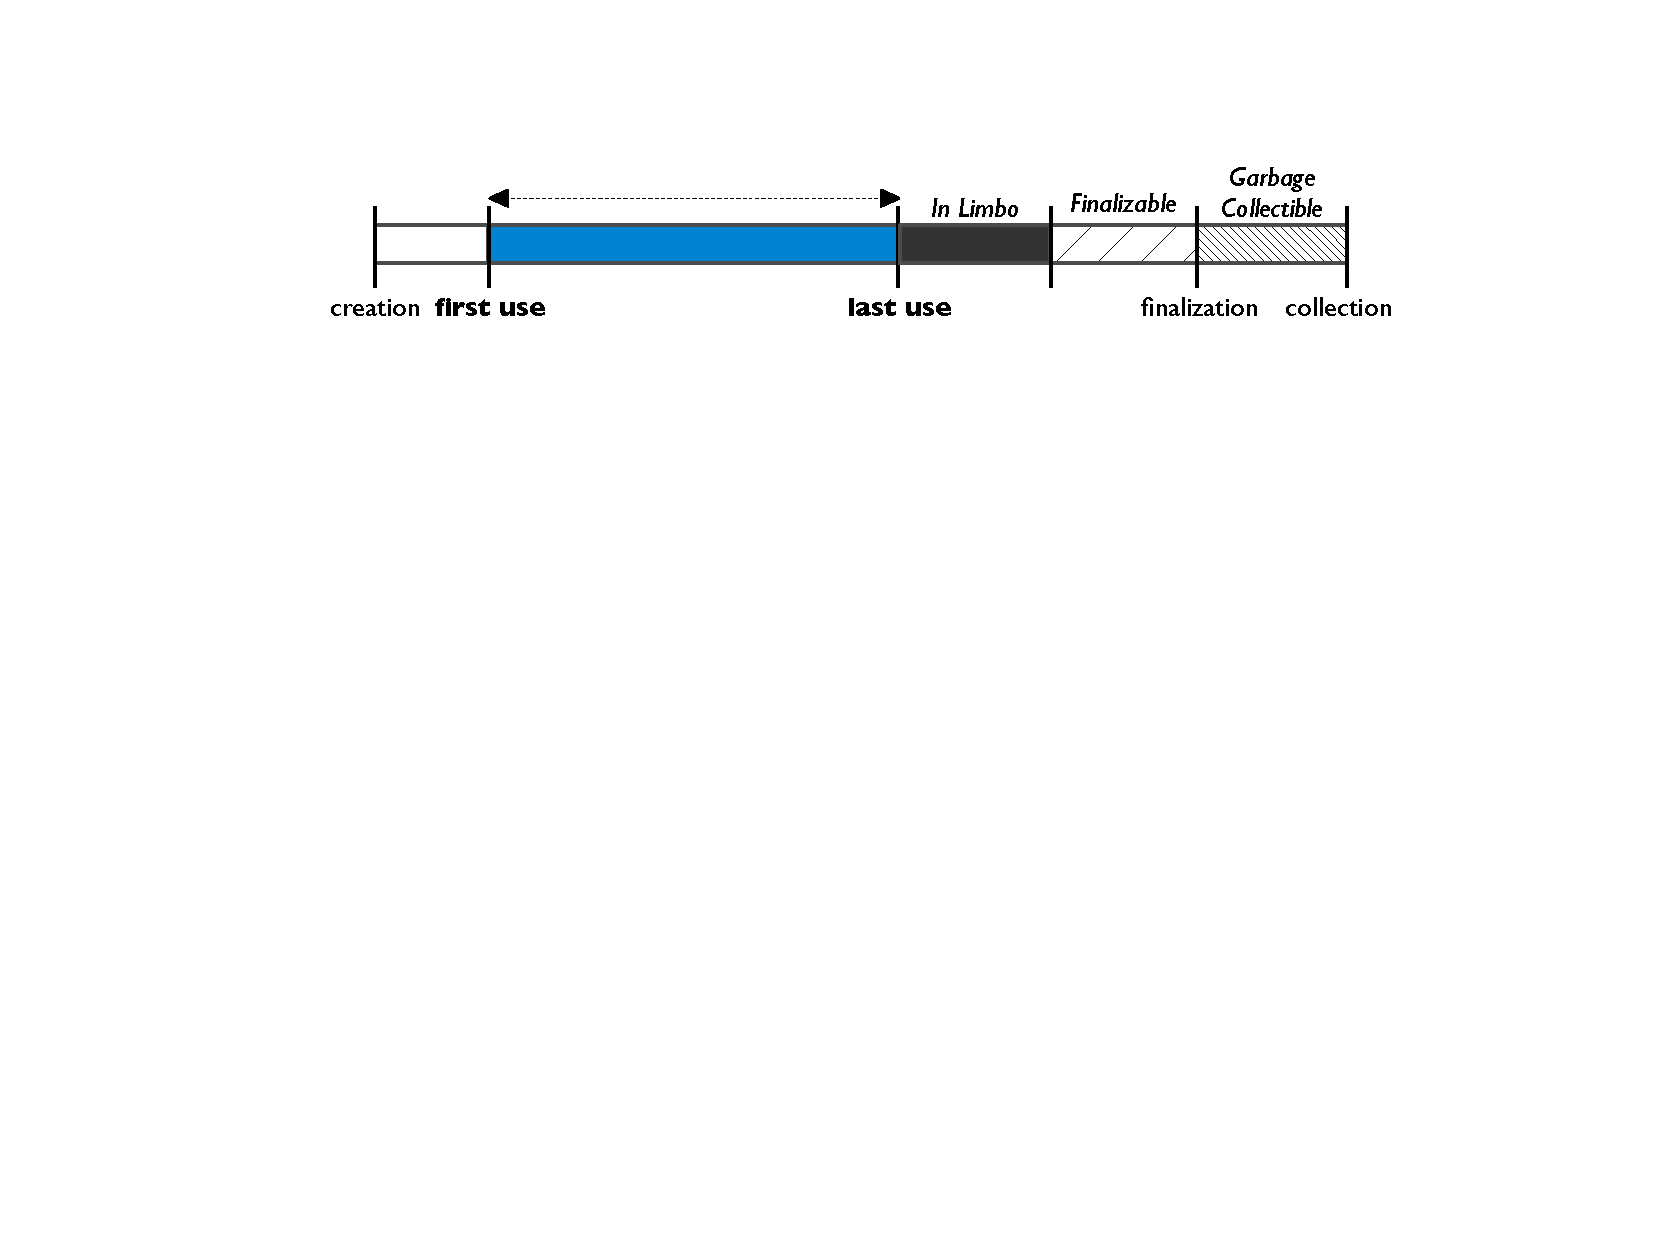
\includegraphics[width=0.9\textwidth]{part4/Figures/lifetime/object-lifecycle}
	\caption{Timeline of the life of an object.}
	\label{fig:typical-lifecycle}
\end{figure}

\begin{example}{Parsing a Date} Consider a loop that shows an easy way to parse
a list of dates. What objects are created, and what are their lifetimes?
\begin{shortlisting}
for (String string : inputList) {
	ParsePosition pos = new ParsePosition(0);
	SimpleDateFormat parser = new SimpleDateFormat();
	System.out.println(parser.parse(string, pos));
}
\end{shortlisting}
\end{example}

For each iteration of this loop, this code takes a date that is represented as a
string and produces a standard Java \class{Date} object. In doing so, a number of
objects are created. Two of these are easy to see, in the two \code{new} calls
that create the parse position and date parser objects. The programmer who wrote
this created two objects, but many more are created by the standard libraries to
finish the task. These include a calendar object, number of arrays, and the
\class{Date} itself. None of these objects are used beyond the iteration of the
loop in which they were created. Within one iteration, they are created, almost
immediately used, and then enter a state of \emph{limbo}.

\callout{limbo}{Objects in Limbo}{
\index{Limbo}
In limbo, an object will never be used again, or at least not for long time,
but the \jre doesn't yet know that this is the case. The object hangs
around, taking up space in the Java heap until the point when it exits limbo.}

The \code{pos} object represents to the parser the position within the
input string to begin parsing. The implementation of the \code{parse} method
uses it early on in the process of parsing. Despite being unused for the
remainder of the parsing, the \jre does not know this until the current
iteration of the loop has finished. This time in limbo also includes the
entirety of the call to \code{System.out.println}, an operation entirely
unrelated to the creation or use of the parse position object. Once the current
loop iteration finishes, these two objects will exit limbo, and become garbage
collectible.\index{Exiting Limbo}

\begin{figure}
	\centering
	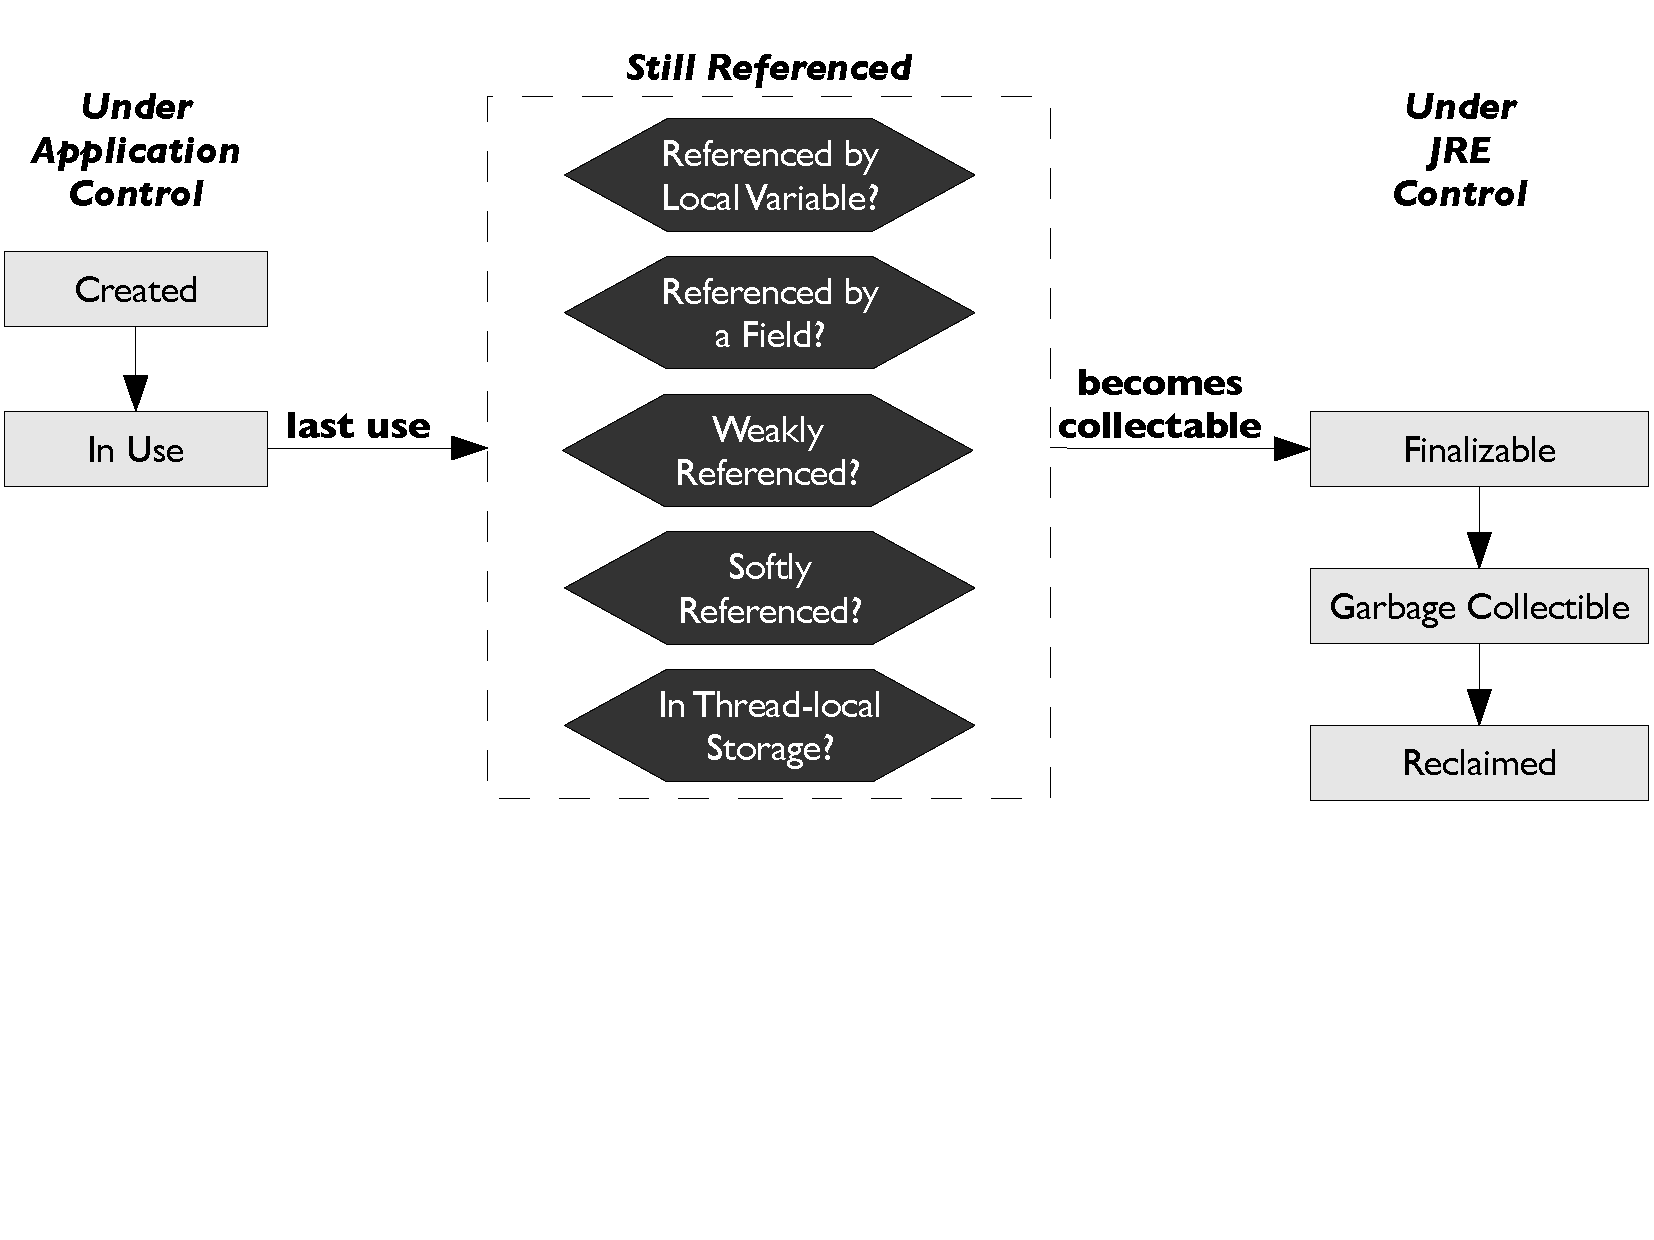
\includegraphics[width=\textwidth]{part4/Figures/lifetime/states}
	\caption{After its last use, an object enters a kind of limbo: the application
	is done with it, but the \jre hasn't yet inferred this to be the case. When an
	object exits limbo depends on the way it is referenced.}
		\label{fig:limbo-exit}
\end{figure}


\begin{comment}
\begin{figure}
	\centering
	\subfigure[The lifecycle of a typical object and its data.]{
	\label{fig:typical-lifecycle1}
			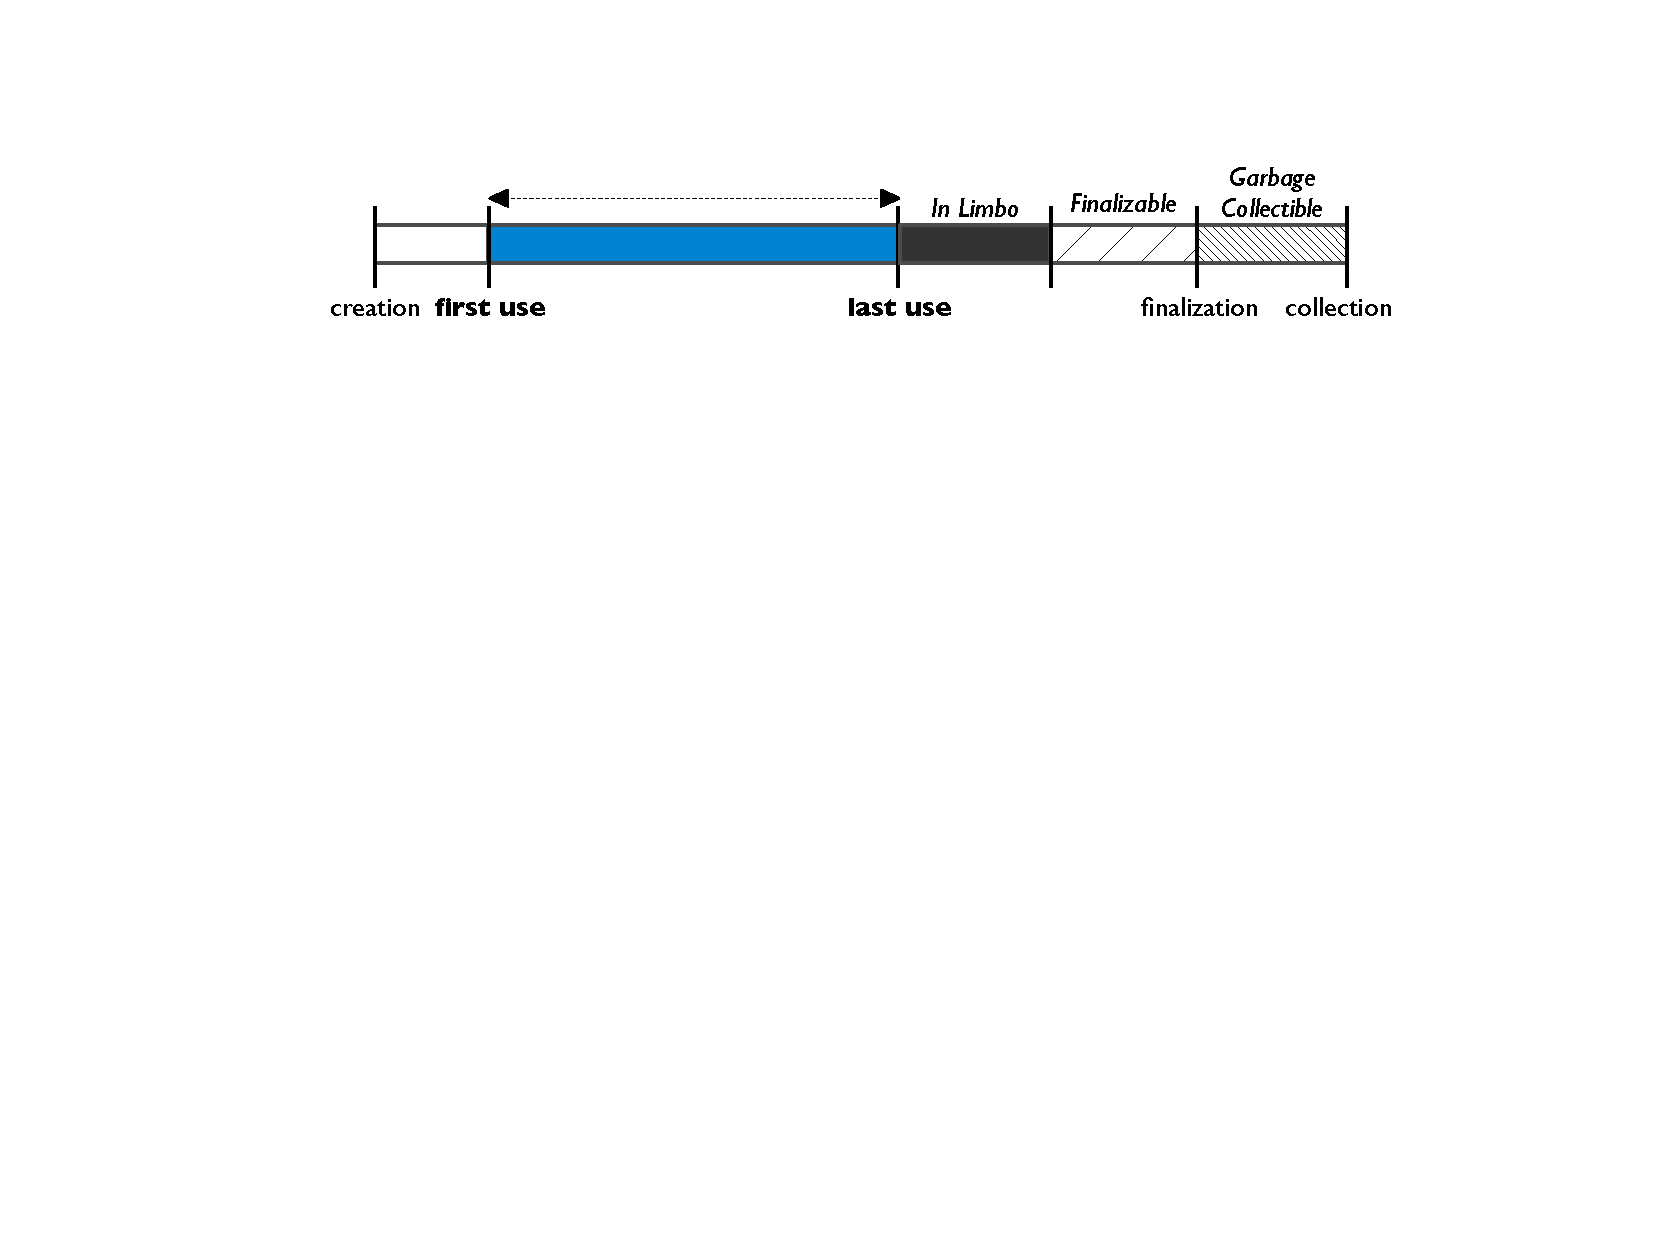
\includegraphics[width=0.95\textwidth]{part4/Figures/lifetime/object-lifecycle}
	}
	\subfigure[A situation where there are long periods between uses of an
	object's data.]{
	\label{fig:typical-lifecycle2}
		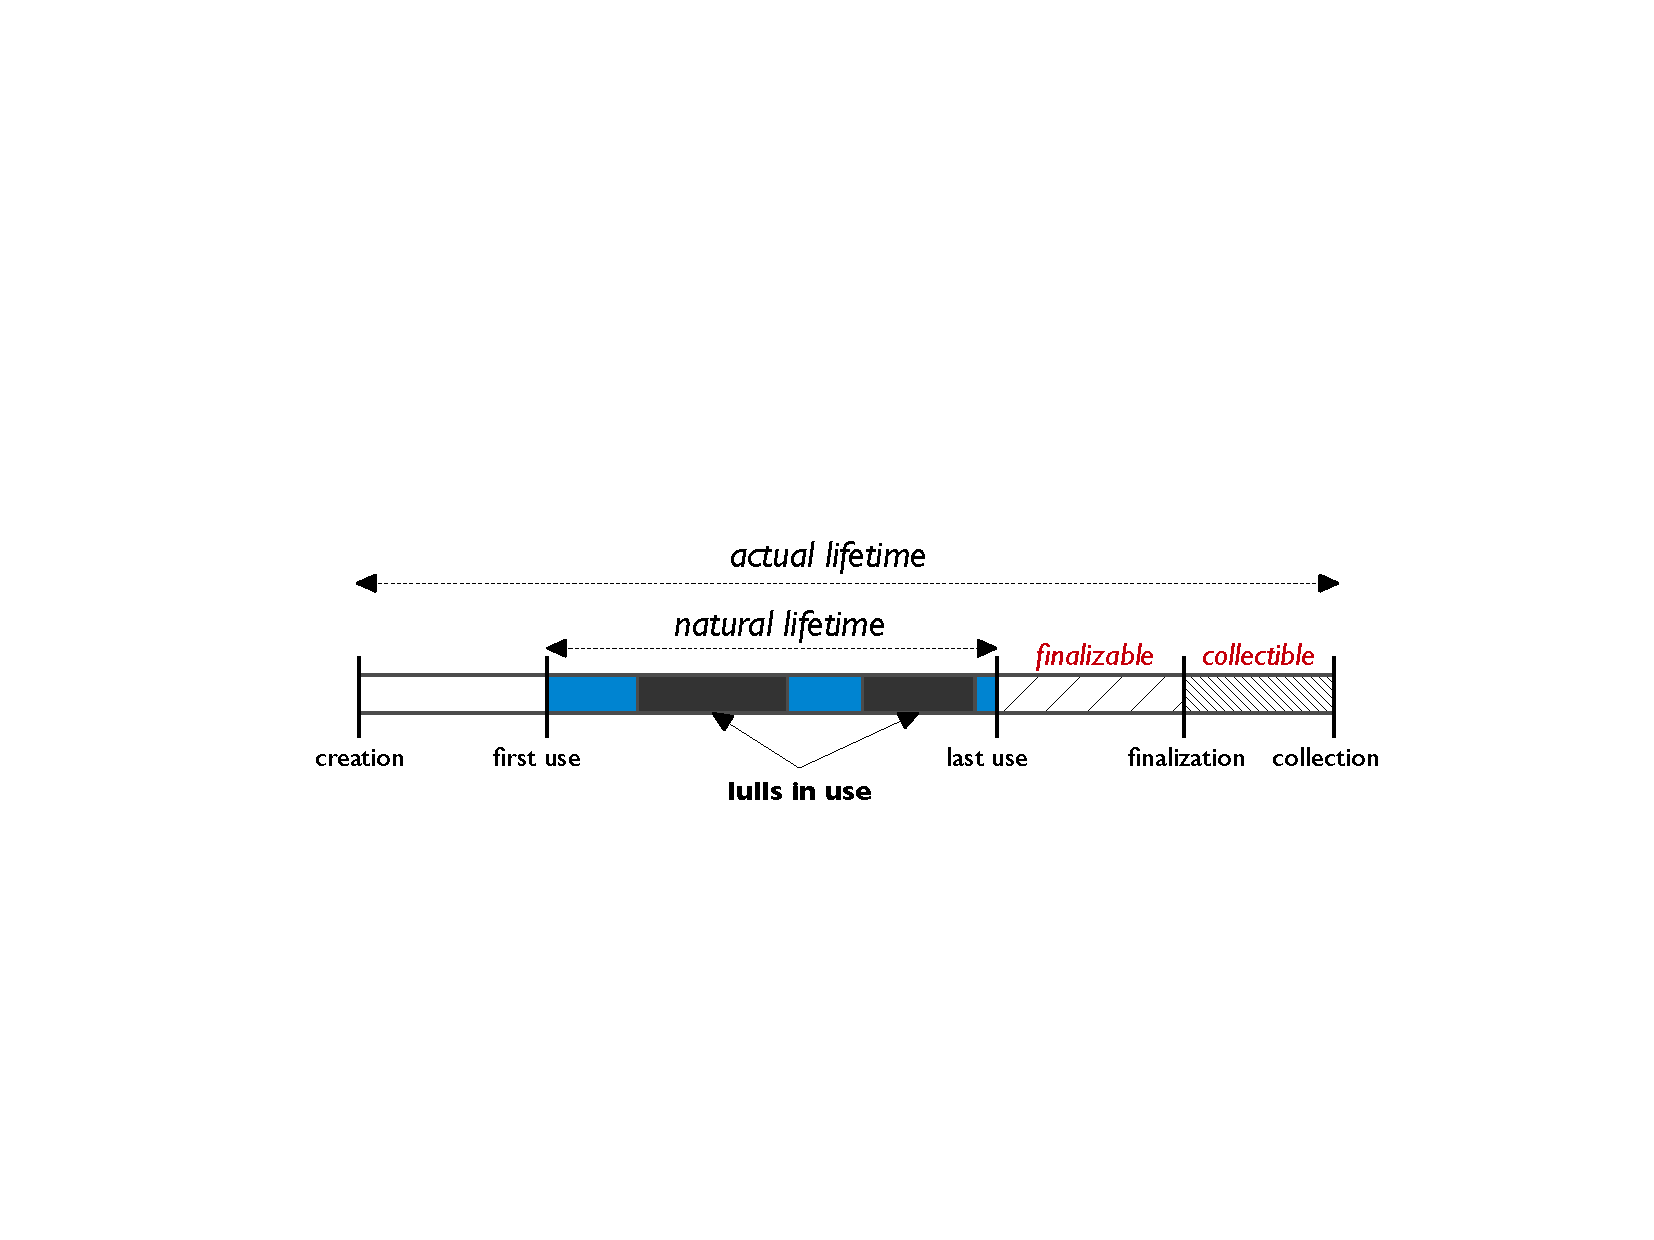
\includegraphics[width=0.95\textwidth]{part4/Figures/lifetime/object-lifecycle-lulls}
	}
	\subfigure[The lifecycle of the data  that is loaded from
	disk three times, and the objects that store it.]{
	\label{fig:typical-lifecycle3}
		\includegraphics[width=0.9\textwidth]{part4/Figures/object-lifecycle2}
	}
	\caption{Examples of Natural and Actual lifetimes.}
	\label{fig:typical-lifecycle}
\end{figure}
\end{comment}


\section{Basic Management Mechanisms}
DO WE NEED THIS?

The point at which an object exits its limbo depends upon how it is referenced by
other objects. One can always assure that an object exits limbo by modifying your
code to overwrite all references to that variable. If an object is no longer
referenced at all, then it will exit limbo immediately.\footnote{Talk about
reference cycles?} For example, a common way to do this is by assigning
references to the value \code{null}. This is tricky in many cases, because it may not be easy to
know where all those references emanate from. Who is to say that, when one calls
the \code{parse} method of a \class{SimpleDateFormat} object, that it does not
squirrel away a reference to the \class{ParsePosition} passed as a parameter? The
API contract for \code{parse} makes no such claims, one way or the other. This is
certainly calls to mind the worst of the days of explicitly managing memory in a
language like C.


Still, one can't always rely on automatic mechanisms to guide an object out of
limbo in a timely fashion.
\autoref{fig:limbo-exit} and \autoref{tab:limbo-exit}
illustrate how an object may exit limbo. 
A garbage collector only knows that an object is ready to
be collected based on {\em reachability}: how the objects point to eachother.
If, as in the \class{ParsePosition}
or \class{SimpleDateFormat} objects from our example, the object is referenced
only by a local variable of a method, the \jre will not consider reclaming its
storage until the variable's scope exits; e.g. when the loop continues to the
next iteration, or when the method returns, depending on the scope of the
variable that references the object. If the object is referenced only by a
field of another object, then it must wait for that other object to exit limbo
before it can do so. 
An objects pointed to be only by a static field has a good chance of never
being collected. A class only exits limbo when it is unloaded by the \jres
class loading mechanism, which is unlikely to happen if it has static fields
that reference other objects. Therefore, unless that field is overwritten,
objects pointed to by static fields are likely never to exit limbo.
\section{Balancing Time and Space}
\label{balance-time-and-space}

sometimes we extend lifetime to optimize (for time)

sometimes we shorten lifetime to optimize (for space)



\begin{table}
\centering
\begin{tabular}{|l|l|} \hline
\em mechanism & \\ \hline \hline
resource pool & \\ \hline
cache & \\ \hline
sharing pool & (interning)\\ \hline
memoization & \\ \hline
backing store &(externalized memo) \\ \hline
non-OO & (column orientation) \\ \hline 
\end{tabular}
\caption{Lifetime management mechanisms not provided by the Java language that one must implement.}
\label{tab:software-lifetime-management}
\end{table}

\chapter{Correlated Lifetimes}

Designing a lifetime management strategy
requires that you take the tools that Java provides, and combine them
with other strategies implemented on top of Java. The built-in mechanisms,
nominally, handle some of the common patterns of object lifetime.
Unfortunately, they often appear in the form of low-level JVM hooks, and so
require careful coding to make correct use of them.  






\section{Basic Management Mechanisms}

The point at which an object exits its limbo depends upon how it is referenced by
other objects. One can always assure that an object exits limbo by modifying your
code to overwrite all references to that variable. If an object is no longer
referenced at all, then it will exit limbo immediately.\footnote{Talk about
reference cycles?} For example, a common way to do this is by assigning
references to the value \code{null}. This is tricky in many cases, because it may not be easy to
know where all those references emanate from. Who is to say that, when one calls
the \code{parse} method of a \class{SimpleDateFormat} object, that it does not
squirrel away a reference to the \class{ParsePosition} passed as a parameter? The
API contract for \code{parse} makes no such claims, one way or the other. This is
certainly calls to mind the worst of the days of explicitly managing memory in a
language like C.


\begin{table}
\centering
	\begin{tabular}{ll} \toprule reachable only from  & moment
	when object exits limbo \\ \cmidrule(r){1-1} \cmidrule(l){2-2}
			%
			nothing & immediately
        	\\
        	%
        	local variable & after scope exits
        	\\ \addlinespace
        	%
        	instance field of an object & 
        	when that object exits limbo %(could be \emph{never} --- memory leak)
        	\\
        	%
        	static field of an object &
        	when that object's class is unloaded
        	%
        	\\ \addlinespace
        	field of \class{WeakReference} & immediately
        	\\
        	%
        	field of \class{SoftReference} & approximately
        	LRU%$^{**}$
        	%
        	\\
        	$\ldots$ with \class{ReferenceQueue} & $\ldots$ then, after removed
        	from queue
        	%
        	\\ \addlinespace
        	entry in thread local storage & when that thread dies
        	%
        	\\ 
        \bottomrule
    \end{tabular}
	\caption{When, or
	even whether, an object exits limbo depends upon how your program references
	it. If these references aren't explicitly overwritten, e.g. by your
	code expliclty assigning the reference to \code{null}, then an object only
	exits limbo under certain restricted circumstances.
%	The point when an object exits limbo depends on 
	%decisions under programmer control: it depends on how the object is
	%referenced.
	%older {\jre}s	use very poor heuristics for handling soft references; see the
	% body for more detail.
	%, it will be reclaimed
	%under certain rules, or may be part of a memory leak
	}
	\label{tab:limbo-exit}
\end{table}

Still, one can't always rely on automatic mechanisms to guide an object out of
limbo in a timely fashion.
\autoref{fig:limbo-exit} and \autoref{tab:limbo-exit}
illustrate how an object may exit limbo. 
A garbage collector only knows that an object is ready to
be collected based on {\em reachability}: how the objects point to eachother.
If, as in the \class{ParsePosition}
or \class{SimpleDateFormat} objects from our example, the object is referenced
only by a local variable of a method, the \jre will not consider reclaming its
storage until the variable's scope exits; e.g. when the loop continues to the
next iteration, or when the method returns, depending on the scope of the
variable that references the object. If the object is referenced only by a
field of another object, then it must wait for that other object to exit limbo
before it can do so. 
An objects pointed to be only by a static field has a good chance of never
being collected. A class only exits limbo when it is unloaded by the \jres
class loading mechanism, which is unlikely to happen if it has static fields
that reference other objects. Therefore, unless that field is overwritten,
objects pointed to by static fields are likely never to exit limbo.

\section{More Complex Management Mechanisms}
There are important lifetime management policies that are not expressible via the
normal mechanisms. When referenced by a local variable, an object lives or dies
with the scope of the variable; when referenced by another object, it lives or
dies along with that object (both, of course, in the absence of overwriting a
reference). The Java specification provides three other mechanisms that let you
guide the \jre to the right time for an object to exit limbo: weak references,
soft references, and thread-local storage.

\subsection{Weak References}
\index{Weak Reference}

Java provides a low-level mechanism that one can use to implement a
correlated lifetime memory management policy, in the form of weak references.
The standard library exposes this feature in the class
\class{java.util.WeakReference}. Using this class correctly is
difficult, because the semantics of weak references does not directly map to
any important application-level use cases.

\begin{definition}
When calling the constructor \class{new WeakReference(obj)},
 this new instance will maintain a reference to \code{obj}, however
 \code{obj} will exit limbo, and become a candidate for cleanup processing by 
the \jre, as if that reference did not exist.
\end{definition} 

When used in this way, weak references don't keep an object alive longer than it
otherwise would have, in the absence of weak references. 
This seems pretty far from anything an application might
need. Still, you can use this low-level feature to implemented correlated
lifetime, as long as you're careful. 
When used to implement correlated lifetime policies, weak references may
indeed delay the time till an object exits limbo.
Improper use of a \class{WeakReference} will
render your code worse off than before. It is quite possible that you will not
have achieved the correlated lifetime that you need, but in a way that is hard
to tell. Even worse, when using weak references, you can introduce memory
leaks. Be very cautious when using them, and follow these rules.

\callout{weaks}{Rules for Using \class{java.util.WeakReference}}{
	In order to assure that you use of weak references works properly, you must
	follow three rules:
	\begin{itemize}
      \item Your instances of \class{WeakReference} must not, directly or
      indirectly, maintain a non-weak reference to the object you wish to
      annotate. It is best to maintain a collection of non-weak references to
      the annotated objects, and use a local variable, or a subclass of
      \class{WeakReference} for any other ways you refer to the annotated object.
      
      \item You must ensure that the \class{WeakReference} objects (or
      subclasses thereof) that you create will exit limbo no sooner than the
      annotated objects. Otherwise, these objects themselves, following the
      rules of \autoref{tab:limbo-exit}, will exit limbo too early. So, if the
      annotated objects are referenced by a collection that is in turn
      referenced by a static field, then the same must be true for the weak
      reference objects as well. 

      \item Since you have to maintain two, parallel, collections to maintain
      references to the annotated objects, and to the annotations, you must
      ensure that exit limbo in lockstep. It is best to create your instances
      of \class{WeakReference} with a \class{ReferenceQueue} parameter. You
      must periodically call \code{poll} on this queue, and remove the
      \class{WeakReference} instances from the parallel registry.
    \end{itemize}
}

You can see that, despite the benefit of some support from the \jre, there
is quite a bit of memory management that you are left with. Luckly, the
standard library ships with a \class{WeakHashMap}\index{WeakHashMap} which deals
with some, but not all, of the legwork of managing weak references. It will
handle the second and third items, but not the first. It is still up to you to
ensure that none of your annotations, directly or indirectly, reference the
annotated object. 

\begin{example}{Timestamp Annotation}
How can you associate a timestamp with an object in a way that avoids memory
leaks and that scales well to a highly concurrent workload?
\end{example}

We can start with the following code:

\begin{shortlisting}
class TimestampAnnotation<T> {
	T t;
	long timestamp;
}
List annotations;
for (String string : inputList) {
	...
	annotations.add(new WeakReference(new Wrapper<String>(string)));
	...
}
\end{shortlisting}

Despite your use of \class{WeakReference}, you would find that neither the main
object (the strings), nor the annotations, would ever be collected. This code
has two memory leaks. One of the leaks is due to a
violation of the first principal of the use of weak references: the annotations
strongly reference the objects being annotated. It is not always this easy to
debug problems in using weak references. Your application will hold on to objects
that you didn't expect. Quite often, it is difficult to even know that there is a
problem in the first place! The application may behave normally, except that it
will consume more memory than necessary; if this extra memory consumption pushes
it over your maximum heap size, then your application will crash --- you will
know something is wrong, but diagnosing this type of problem, a memory
leak\index{Memory Leak}, is quite difficult. It is better to keep the
three principles of weak references in mind, and design in a way that avoids
memory leaks in the first place. Your annotations can be modified to use a
\class{WeakReference} to the main object:

\begin{shortlisting}
class TimestampAnnotation<T> {
	WeakReference<T> t; // annotation only weakly refs main object
	long timestamp;
	
	TimestampAnnotation(T t) {
		this.t = new WeakReference(t);
	}
}
\end{shortlisting}

In this case, the annotation has no normal references to the annotated object,
and so it obides by the first rule of weak references. If you remember from
\autoref{chapter:delegation}, the code can be improved further to avoid the cost
of delegation. This version of the annotation class extends
\class{WeakReference}:

\begin{shortlisting}
class TimestampAnnotation<T> extends WeakReference<T> {
	long timestamp;
	
	TimestampAnnotation(T t) {
		super(t);
	}
}
\end{shortlisting}

Unfortunately, both of these updated versions h

\subsection{Soft References}
\index{Soft Reference}

\subsection{Properly Draining a Reference Queue}

\subsection{Thread-local Storage}
\index{Thread-local Storage}

%about objects not information; we can discuss in outside the box the issue of
%information needed forver but shuttled in and out.

\chapter{Outside the Java Box}
\label{chapter:outisde-java-box}

\begin{example}{Nodes and Edges}

\end{example}

\section{The Bulk Sharing Pool}
\label{sec:bulk-sharing-pool}

The
bulk storage that backs a set of data items, each of the same type.
Objects share
the data by indexing into the pool.

\section{Column-oriented Storage}

\section{Representing Relationships}

\section{Memory Mapping}
%\chapter{Lifetime Management in Other Languages}

\section{C++: Smart Pointers}

\code{auto\_ptr}, single-owner notion, auto-free

\section{C\#: Value Types}

\section{Ada95: Storage Pools}


%Bugs, performance problems, memory footprint.




%Story
%-------
%data has a natural lifetime
	%you can use the above mechanisms to manage
%sometimes we extend lifetime to optimize (for time)
%sometimes we shorten lifetime to optimize (for space)


%Problems:
	%Temps -- saving time
	%Making things fit
		%Things you need
		%Things you can recompute

		
		
		
%Chapter 1: Natural Lifetimes
	%- if scopes don't coincide with lifetime
	%- actual lifetime may be different from natural lifetime, for performance reasons
%Chapter 2: Getting Lifetime Correct
%Chapter 3: Getting It Small and Fast



\appendix

\chapter{Tools to Help with Memory Analysis}
\label{chapter:tools}

%%%%%%%%%%%%%%%%%%%%%%%%
%%%%   BACK MATTER  %%%%
%%%%%%%%%%%%%%%%%%%%%%%%
\backmatter

%\bibliographystyle{abbrv}
\bibliographystyle{unsrt}
\bibliography{bloat}

\printindex

\end{document}
